\documentclass[twoside]{book}

% Packages required by doxygen
\usepackage{fixltx2e}
\usepackage{calc}
\usepackage{doxygen}
\usepackage[export]{adjustbox} % also loads graphicx
\usepackage{graphicx}
\usepackage[utf8]{inputenc}
\usepackage{makeidx}
\usepackage{multicol}
\usepackage{multirow}
\PassOptionsToPackage{warn}{textcomp}
\usepackage{textcomp}
\usepackage[nointegrals]{wasysym}
\usepackage[table]{xcolor}

% Font selection
\usepackage[T1]{fontenc}
\usepackage[scaled=.90]{helvet}
\usepackage{courier}
\usepackage{amssymb}
\usepackage{sectsty}
\renewcommand{\familydefault}{\sfdefault}
\allsectionsfont{%
  \fontseries{bc}\selectfont%
  \color{darkgray}%
}
\renewcommand{\DoxyLabelFont}{%
  \fontseries{bc}\selectfont%
  \color{darkgray}%
}
\newcommand{\+}{\discretionary{\mbox{\scriptsize$\hookleftarrow$}}{}{}}

% Page & text layout
\usepackage{geometry}
\geometry{%
  a4paper,%
  top=2.5cm,%
  bottom=2.5cm,%
  left=2.5cm,%
  right=2.5cm%
}
\tolerance=750
\hfuzz=15pt
\hbadness=750
\setlength{\emergencystretch}{15pt}
\setlength{\parindent}{0cm}
\setlength{\parskip}{3ex plus 2ex minus 2ex}
\makeatletter
\renewcommand{\paragraph}{%
  \@startsection{paragraph}{4}{0ex}{-1.0ex}{1.0ex}{%
    \normalfont\normalsize\bfseries\SS@parafont%
  }%
}
\renewcommand{\subparagraph}{%
  \@startsection{subparagraph}{5}{0ex}{-1.0ex}{1.0ex}{%
    \normalfont\normalsize\bfseries\SS@subparafont%
  }%
}
\makeatother

% Headers & footers
\usepackage{fancyhdr}
\pagestyle{fancyplain}
\fancyhead[LE]{\fancyplain{}{\bfseries\thepage}}
\fancyhead[CE]{\fancyplain{}{}}
\fancyhead[RE]{\fancyplain{}{\bfseries\leftmark}}
\fancyhead[LO]{\fancyplain{}{\bfseries\rightmark}}
\fancyhead[CO]{\fancyplain{}{}}
\fancyhead[RO]{\fancyplain{}{\bfseries\thepage}}
\fancyfoot[LE]{\fancyplain{}{}}
\fancyfoot[CE]{\fancyplain{}{}}
\fancyfoot[RE]{\fancyplain{}{\bfseries\scriptsize Generated by Doxygen }}
\fancyfoot[LO]{\fancyplain{}{\bfseries\scriptsize Generated by Doxygen }}
\fancyfoot[CO]{\fancyplain{}{}}
\fancyfoot[RO]{\fancyplain{}{}}
\renewcommand{\footrulewidth}{0.4pt}
\renewcommand{\chaptermark}[1]{%
  \markboth{#1}{}%
}
\renewcommand{\sectionmark}[1]{%
  \markright{\thesection\ #1}%
}

% Indices & bibliography
\usepackage{natbib}
\usepackage[titles]{tocloft}
\setcounter{tocdepth}{3}
\setcounter{secnumdepth}{5}
\makeindex

% Hyperlinks (required, but should be loaded last)
\usepackage{ifpdf}
\ifpdf
  \usepackage[pdftex,pagebackref=true]{hyperref}
\else
  \usepackage[ps2pdf,pagebackref=true]{hyperref}
\fi
\hypersetup{%
  colorlinks=true,%
  linkcolor=blue,%
  citecolor=blue,%
  unicode%
}

% Custom commands
\newcommand{\clearemptydoublepage}{%
  \newpage{\pagestyle{empty}\cleardoublepage}%
}

\usepackage{caption}
\captionsetup{labelsep=space,justification=centering,font={bf},singlelinecheck=off,skip=4pt,position=top}

%===== C O N T E N T S =====

\begin{document}

% Titlepage & ToC
\hypersetup{pageanchor=false,
             bookmarksnumbered=true,
             pdfencoding=unicode
            }
\pagenumbering{alph}
\begin{titlepage}
\vspace*{7cm}
\begin{center}%
{\Large E\+C\+M\+A\+Script }\\
\vspace*{1cm}
{\large Generated by Doxygen 1.8.13}\\
\end{center}
\end{titlepage}
\clearemptydoublepage
\pagenumbering{roman}
\tableofcontents
\clearemptydoublepage
\pagenumbering{arabic}
\hypersetup{pageanchor=true}

%--- Begin generated contents ---
\chapter{Namespace Index}
\section{Namespace List}
Here is a list of all namespaces with brief descriptions\+:\begin{DoxyCompactList}
\item\contentsline{section}{\hyperlink{namespaceast}{ast} }{\pageref{namespaceast}}{}
\end{DoxyCompactList}

\chapter{Hierarchical Index}
\section{Class Hierarchy}
This inheritance list is sorted roughly, but not completely, alphabetically\+:\begin{DoxyCompactList}
\item \contentsline{section}{Basic\+Lexer$<$ T $>$}{\pageref{class_basic_lexer}}{}
\item \contentsline{section}{B\+Cinfo}{\pageref{struct_b_cinfo}}{}
\item \contentsline{section}{B\+F96}{\pageref{struct_b_f96}}{}
\item \contentsline{section}{Bigint}{\pageref{struct_bigint}}{}
\item \contentsline{section}{Binding}{\pageref{struct_binding}}{}
\item \contentsline{section}{Boolean}{\pageref{struct_boolean}}{}
\item \contentsline{section}{Token\+:\+:Debug\+Info}{\pageref{struct_token_1_1_debug_info}}{}
\item \contentsline{section}{Environment\+Record}{\pageref{struct_environment_record}}{}
\begin{DoxyCompactList}
\item \contentsline{section}{Declarative\+Environment\+Record}{\pageref{struct_declarative_environment_record}}{}
\item \contentsline{section}{Declarative\+Environment\+Record}{\pageref{struct_declarative_environment_record}}{}
\item \contentsline{section}{Object\+Environment\+Record}{\pageref{struct_object_environment_record}}{}
\end{DoxyCompactList}
\item \contentsline{section}{Execution\+Context}{\pageref{struct_execution_context}}{}
\item std\+:\+:hash$<$ std\+:\+:u16string $>${\ttfamily  \mbox{[}external\mbox{]}}\begin{DoxyCompactList}
\item \contentsline{section}{std\+:\+:hash$<$ String $>$}{\pageref{structstd_1_1hash_3_01_string_01_4}}{}
\end{DoxyCompactList}
\item \contentsline{section}{Input\+Element}{\pageref{class_input_element}}{}
\item \contentsline{section}{Lexical\+Environment}{\pageref{struct_lexical_environment}}{}
\item \contentsline{section}{Lexical\+Grammar$<$ T $>$}{\pageref{class_lexical_grammar}}{}
\item \contentsline{section}{Logger}{\pageref{class_logger}}{}
\begin{DoxyCompactList}
\item \contentsline{section}{Silent\+Logger}{\pageref{class_silent_logger}}{}
\item \contentsline{section}{Standard\+Logger$<$ T $>$}{\pageref{class_standard_logger}}{}
\end{DoxyCompactList}
\item \contentsline{section}{Matcher$<$ T, It $>$}{\pageref{class_matcher}}{}
\item \contentsline{section}{Matcher$<$ T, std\+:\+:u16string\+:\+:const\+\_\+iterator $>$}{\pageref{class_matcher}}{}
\item \contentsline{section}{Matcher$<$ Token, std\+:\+:vector$<$ Token $>$\+:\+:iterator $>$}{\pageref{class_matcher}}{}
\item \contentsline{section}{Node}{\pageref{struct_node}}{}
\begin{DoxyCompactList}
\item \contentsline{section}{Array\+Literal}{\pageref{struct_array_literal}}{}
\item \contentsline{section}{Case\+Clause}{\pageref{struct_case_clause}}{}
\begin{DoxyCompactList}
\item \contentsline{section}{Default\+Clause}{\pageref{struct_default_clause}}{}
\end{DoxyCompactList}
\item \contentsline{section}{Elision}{\pageref{struct_elision}}{}
\item \contentsline{section}{Expression}{\pageref{struct_expression}}{}
\begin{DoxyCompactList}
\item \contentsline{section}{Arguments}{\pageref{struct_arguments}}{}
\item \contentsline{section}{Binary\+Expression}{\pageref{struct_binary_expression}}{}
\begin{DoxyCompactList}
\item \contentsline{section}{Assignment\+Expression}{\pageref{struct_assignment_expression}}{}
\end{DoxyCompactList}
\item \contentsline{section}{Call\+Expression}{\pageref{struct_call_expression}}{}
\item \contentsline{section}{Conditional\+Expression}{\pageref{struct_conditional_expression}}{}
\item \contentsline{section}{Function\+Expression}{\pageref{struct_function_expression}}{}
\item \contentsline{section}{Left\+Hand\+Side\+Expression}{\pageref{struct_left_hand_side_expression}}{}
\begin{DoxyCompactList}
\item \contentsline{section}{Primary\+Expression}{\pageref{struct_primary_expression}}{}
\begin{DoxyCompactList}
\item \contentsline{section}{Array\+Expression}{\pageref{struct_array_expression}}{}
\item \contentsline{section}{Identifier\+Expression}{\pageref{struct_identifier_expression}}{}
\item \contentsline{section}{Literal\+Expression}{\pageref{struct_literal_expression}}{}
\item \contentsline{section}{Object\+Expression}{\pageref{struct_object_expression}}{}
\item \contentsline{section}{Object\+Literal}{\pageref{struct_object_literal}}{}
\item \contentsline{section}{This\+Expression}{\pageref{struct_this_expression}}{}
\end{DoxyCompactList}
\end{DoxyCompactList}
\item \contentsline{section}{Member\+Expression}{\pageref{struct_member_expression}}{}
\item \contentsline{section}{New\+Expression}{\pageref{struct_new_expression}}{}
\item \contentsline{section}{Postfix\+Expression}{\pageref{struct_postfix_expression}}{}
\item \contentsline{section}{Property\+Assignment}{\pageref{struct_property_assignment}}{}
\item \contentsline{section}{Property\+Name}{\pageref{struct_property_name}}{}
\item \contentsline{section}{Unary\+Expression}{\pageref{struct_unary_expression}}{}
\item \contentsline{section}{Variable\+Declaration}{\pageref{struct_variable_declaration}}{}
\end{DoxyCompactList}
\item \contentsline{section}{Identifier}{\pageref{struct_identifier}}{}
\item \contentsline{section}{List$<$ T $>$}{\pageref{struct_list}}{}
\item \contentsline{section}{List$<$ Case\+Clause $>$}{\pageref{struct_list}}{}
\begin{DoxyCompactList}
\item \contentsline{section}{Case\+Block}{\pageref{struct_case_block}}{}
\end{DoxyCompactList}
\item \contentsline{section}{List$<$ Expression $>$}{\pageref{struct_list}}{}
\begin{DoxyCompactList}
\item \contentsline{section}{Argument\+List}{\pageref{struct_argument_list}}{}
\end{DoxyCompactList}
\item \contentsline{section}{List$<$ Identifier $>$}{\pageref{struct_list}}{}
\begin{DoxyCompactList}
\item \contentsline{section}{Formal\+Parameter\+List}{\pageref{struct_formal_parameter_list}}{}
\end{DoxyCompactList}
\item \contentsline{section}{List$<$ Node $>$}{\pageref{struct_list}}{}
\begin{DoxyCompactList}
\item \contentsline{section}{Element\+List}{\pageref{struct_element_list}}{}
\end{DoxyCompactList}
\item \contentsline{section}{List$<$ Property\+Assignment $>$}{\pageref{struct_list}}{}
\begin{DoxyCompactList}
\item \contentsline{section}{Property\+Name\+And\+Value\+List}{\pageref{struct_property_name_and_value_list}}{}
\end{DoxyCompactList}
\item \contentsline{section}{List$<$ Source\+Element $>$}{\pageref{struct_list}}{}
\begin{DoxyCompactList}
\item \contentsline{section}{Source\+Elements}{\pageref{struct_source_elements}}{}
\begin{DoxyCompactList}
\item \contentsline{section}{Function\+Body}{\pageref{struct_function_body}}{}
\end{DoxyCompactList}
\end{DoxyCompactList}
\item \contentsline{section}{List$<$ Statement $>$}{\pageref{struct_list}}{}
\begin{DoxyCompactList}
\item \contentsline{section}{Statement\+List}{\pageref{struct_statement_list}}{}
\end{DoxyCompactList}
\item \contentsline{section}{List$<$ Variable\+Declaration $>$}{\pageref{struct_list}}{}
\begin{DoxyCompactList}
\item \contentsline{section}{Variable\+Declaration\+List}{\pageref{struct_variable_declaration_list}}{}
\end{DoxyCompactList}
\item \contentsline{section}{Literal}{\pageref{struct_literal}}{}
\begin{DoxyCompactList}
\item \contentsline{section}{Boolean\+Literal}{\pageref{struct_boolean_literal}}{}
\item \contentsline{section}{Null\+Literal}{\pageref{struct_null_literal}}{}
\item \contentsline{section}{Numeric\+Literal}{\pageref{struct_numeric_literal}}{}
\item \contentsline{section}{Regular\+Expression\+Literal}{\pageref{struct_regular_expression_literal}}{}
\item \contentsline{section}{String\+Literal}{\pageref{struct_string_literal}}{}
\end{DoxyCompactList}
\item \contentsline{section}{Source\+Element}{\pageref{struct_source_element}}{}
\begin{DoxyCompactList}
\item \contentsline{section}{Declaration}{\pageref{struct_declaration}}{}
\begin{DoxyCompactList}
\item \contentsline{section}{Program\+Declaration}{\pageref{struct_program_declaration}}{}
\end{DoxyCompactList}
\item \contentsline{section}{Function\+Declaration}{\pageref{struct_function_declaration}}{}
\item \contentsline{section}{Statement}{\pageref{struct_statement}}{}
\begin{DoxyCompactList}
\item \contentsline{section}{Block}{\pageref{struct_block}}{}
\item \contentsline{section}{Break\+Statement}{\pageref{struct_break_statement}}{}
\item \contentsline{section}{Continue\+Statement}{\pageref{struct_continue_statement}}{}
\item \contentsline{section}{Debugger\+Statement}{\pageref{struct_debugger_statement}}{}
\item \contentsline{section}{Do\+While\+Statement}{\pageref{struct_do_while_statement}}{}
\item \contentsline{section}{Empty\+Statement}{\pageref{struct_empty_statement}}{}
\item \contentsline{section}{Expression\+Statement}{\pageref{struct_expression_statement}}{}
\item \contentsline{section}{For\+In\+Statement}{\pageref{struct_for_in_statement}}{}
\item \contentsline{section}{For\+Statement}{\pageref{struct_for_statement}}{}
\item \contentsline{section}{If\+Statement}{\pageref{struct_if_statement}}{}
\item \contentsline{section}{Labelled\+Statement}{\pageref{struct_labelled_statement}}{}
\item \contentsline{section}{Return\+Statement}{\pageref{struct_return_statement}}{}
\item \contentsline{section}{Switch\+Statement}{\pageref{struct_switch_statement}}{}
\item \contentsline{section}{Throw\+Statement}{\pageref{struct_throw_statement}}{}
\item \contentsline{section}{Try\+Statement}{\pageref{struct_try_statement}}{}
\item \contentsline{section}{Variable\+Statement}{\pageref{struct_variable_statement}}{}
\item \contentsline{section}{While\+Statement}{\pageref{struct_while_statement}}{}
\item \contentsline{section}{With\+Statement}{\pageref{struct_with_statement}}{}
\end{DoxyCompactList}
\end{DoxyCompactList}
\item \contentsline{section}{This}{\pageref{struct_this}}{}
\end{DoxyCompactList}
\item \contentsline{section}{Null}{\pageref{struct_null}}{}
\item \contentsline{section}{Number}{\pageref{struct_number}}{}
\item \contentsline{section}{Object}{\pageref{struct_object}}{}
\item \contentsline{section}{overloaded\+\_\+t$<$ Ts $>$}{\pageref{structoverloaded__t}}{}
\item \contentsline{section}{overloaded\+\_\+t$<$ Ts... $>$}{\pageref{structoverloaded__t}}{}
\begin{DoxyCompactList}
\item \contentsline{section}{overloaded\+\_\+t$<$ T, Ts... $>$}{\pageref{structoverloaded__t_3_01_t_00_01_ts_8_8_8_01_4}}{}
\end{DoxyCompactList}
\item \contentsline{section}{Parser}{\pageref{class_parser}}{}
\item \contentsline{section}{print}{\pageref{structprint}}{}
\item \contentsline{section}{Program}{\pageref{struct_program}}{}
\item \contentsline{section}{Reference}{\pageref{struct_reference}}{}
\item std\+:\+:runtime\+\_\+error{\ttfamily  \mbox{[}external\mbox{]}}\begin{DoxyCompactList}
\item \contentsline{section}{Syntax\+Error}{\pageref{class_syntax_error}}{}
\item \contentsline{section}{Syntax\+Error}{\pageref{class_syntax_error}}{}
\end{DoxyCompactList}
\item \contentsline{section}{Basic\+Lexer$<$ T $>$\+:\+:Tokens\+:\+:storage\+\_\+t}{\pageref{struct_basic_lexer_1_1_tokens_1_1storage__t}}{}
\item \contentsline{section}{String}{\pageref{struct_string}}{}
\item T\begin{DoxyCompactList}
\item \contentsline{section}{overloaded\+\_\+t$<$ T $>$}{\pageref{structoverloaded__t_3_01_t_01_4}}{}
\item \contentsline{section}{overloaded\+\_\+t$<$ T, Ts... $>$}{\pageref{structoverloaded__t_3_01_t_00_01_ts_8_8_8_01_4}}{}
\end{DoxyCompactList}
\item \contentsline{section}{Th\+Info}{\pageref{struct_th_info}}{}
\item \contentsline{section}{Token}{\pageref{class_token}}{}
\item \contentsline{section}{Trace}{\pageref{class_trace}}{}
\item \contentsline{section}{Trace\+Guard}{\pageref{class_trace_guard}}{}
\item \contentsline{section}{Type}{\pageref{class_type}}{}
\item \contentsline{section}{U}{\pageref{union_u}}{}
\item \contentsline{section}{Undefined}{\pageref{struct_undefined}}{}
\item \contentsline{section}{Visitor}{\pageref{struct_visitor}}{}
\begin{DoxyCompactList}
\item \contentsline{section}{Basic\+Visitor}{\pageref{struct_basic_visitor}}{}
\begin{DoxyCompactList}
\item \contentsline{section}{Eval\+Visitor}{\pageref{class_eval_visitor}}{}
\item \contentsline{section}{J\+S\+O\+N\+Visitor}{\pageref{class_j_s_o_n_visitor}}{}
\item \contentsline{section}{Simplified\+Y\+A\+M\+L\+Visitor}{\pageref{class_simplified_y_a_m_l_visitor}}{}
\end{DoxyCompactList}
\item \contentsline{section}{Delegate\+Vistor}{\pageref{struct_delegate_vistor}}{}
\item \contentsline{section}{Lambda\+Visitor$<$ Lambda $>$}{\pageref{struct_lambda_visitor}}{}
\end{DoxyCompactList}
\end{DoxyCompactList}

\chapter{Class Index}
\section{Class List}
Here are the classes, structs, unions and interfaces with brief descriptions\+:\begin{DoxyCompactList}
\item\contentsline{section}{\hyperlink{struct_argument_list}{Argument\+List} }{\pageref{struct_argument_list}}{}
\item\contentsline{section}{\hyperlink{struct_arguments}{Arguments} }{\pageref{struct_arguments}}{}
\item\contentsline{section}{\hyperlink{struct_array_literal}{Array\+Literal} }{\pageref{struct_array_literal}}{}
\item\contentsline{section}{\hyperlink{class_basic_lexer}{Basic\+Lexer$<$ T $>$} }{\pageref{class_basic_lexer}}{}
\item\contentsline{section}{\hyperlink{struct_binary_expression}{Binary\+Expression} }{\pageref{struct_binary_expression}}{}
\item\contentsline{section}{\hyperlink{struct_block}{Block} }{\pageref{struct_block}}{}
\item\contentsline{section}{\hyperlink{struct_boolean}{Boolean} }{\pageref{struct_boolean}}{}
\item\contentsline{section}{\hyperlink{struct_boolean_literal}{Boolean\+Literal} }{\pageref{struct_boolean_literal}}{}
\item\contentsline{section}{\hyperlink{struct_break_statement}{Break\+Statement} }{\pageref{struct_break_statement}}{}
\item\contentsline{section}{\hyperlink{struct_callable_visitor}{Callable\+Visitor$<$ Callable $>$} }{\pageref{struct_callable_visitor}}{}
\item\contentsline{section}{\hyperlink{struct_call_expression}{Call\+Expression} }{\pageref{struct_call_expression}}{}
\item\contentsline{section}{\hyperlink{struct_case_block}{Case\+Block} }{\pageref{struct_case_block}}{}
\item\contentsline{section}{\hyperlink{struct_case_clause}{Case\+Clause} }{\pageref{struct_case_clause}}{}
\item\contentsline{section}{\hyperlink{struct_conditional_expression}{Conditional\+Expression} }{\pageref{struct_conditional_expression}}{}
\item\contentsline{section}{\hyperlink{struct_continue_statement}{Continue\+Statement} }{\pageref{struct_continue_statement}}{}
\item\contentsline{section}{\hyperlink{struct_debugger_statement}{Debugger\+Statement} }{\pageref{struct_debugger_statement}}{}
\item\contentsline{section}{\hyperlink{struct_token_1_1_debug_info}{Token\+::\+Debug\+Info} }{\pageref{struct_token_1_1_debug_info}}{}
\item\contentsline{section}{\hyperlink{struct_declaration}{Declaration} }{\pageref{struct_declaration}}{}
\item\contentsline{section}{\hyperlink{struct_default_clause}{Default\+Clause} }{\pageref{struct_default_clause}}{}
\item\contentsline{section}{\hyperlink{struct_do_while_statement}{Do\+While\+Statement} }{\pageref{struct_do_while_statement}}{}
\item\contentsline{section}{\hyperlink{struct_element_list}{Element\+List} }{\pageref{struct_element_list}}{}
\item\contentsline{section}{\hyperlink{struct_elision}{Elision} }{\pageref{struct_elision}}{}
\item\contentsline{section}{\hyperlink{struct_empty_statement}{Empty\+Statement} }{\pageref{struct_empty_statement}}{}
\item\contentsline{section}{\hyperlink{struct_token_1_1equal__visitor}{Token\+::equal\+\_\+visitor} }{\pageref{struct_token_1_1equal__visitor}}{}
\item\contentsline{section}{\hyperlink{struct_expression}{Expression} }{\pageref{struct_expression}}{}
\item\contentsline{section}{\hyperlink{struct_expression_statement}{Expression\+Statement} }{\pageref{struct_expression_statement}}{}
\item\contentsline{section}{\hyperlink{struct_for_in_statement}{For\+In\+Statement} }{\pageref{struct_for_in_statement}}{}
\item\contentsline{section}{\hyperlink{struct_formal_parameter_list}{Formal\+Parameter\+List} }{\pageref{struct_formal_parameter_list}}{}
\item\contentsline{section}{\hyperlink{struct_for_statement}{For\+Statement} }{\pageref{struct_for_statement}}{}
\item\contentsline{section}{\hyperlink{struct_function_body}{Function\+Body} }{\pageref{struct_function_body}}{}
\item\contentsline{section}{\hyperlink{struct_function_declaration}{Function\+Declaration} }{\pageref{struct_function_declaration}}{}
\item\contentsline{section}{\hyperlink{struct_function_expression}{Function\+Expression} }{\pageref{struct_function_expression}}{}
\item\contentsline{section}{\hyperlink{struct_identifier}{Identifier} }{\pageref{struct_identifier}}{}
\item\contentsline{section}{\hyperlink{struct_if_statement}{If\+Statement} }{\pageref{struct_if_statement}}{}
\item\contentsline{section}{\hyperlink{structindentstream}{indentstream} }{\pageref{structindentstream}}{}
\item\contentsline{section}{\hyperlink{class_input_element}{Input\+Element} }{\pageref{class_input_element}}{}
\item\contentsline{section}{\hyperlink{structdetail_1_1is__callable1}{detail\+::is\+\_\+callable1$<$ class, class, class $>$} }{\pageref{structdetail_1_1is__callable1}}{}
\item\contentsline{section}{\hyperlink{structdetail_1_1is__callable1_3_01_t_00_01_f_00_01void__t_3_01decltype_07std_1_1declval_3_01_f_0031734589d10bdb36da443f727c3d6f8}{detail\+::is\+\_\+callable1$<$ T, F, void\+\_\+t$<$ decltype(std\+::declval$<$ F $>$()(std\+::declval$<$ T $>$()))$>$ $>$} }{\pageref{structdetail_1_1is__callable1_3_01_t_00_01_f_00_01void__t_3_01decltype_07std_1_1declval_3_01_f_0031734589d10bdb36da443f727c3d6f8}}{}
\item\contentsline{section}{\hyperlink{structdetail_1_1is__callable2}{detail\+::is\+\_\+callable2$<$ class, class, class, class $>$} }{\pageref{structdetail_1_1is__callable2}}{}
\item\contentsline{section}{\hyperlink{structdetail_1_1is__callable2_3_01_t_00_01_n_00_01_f_00_01void__t_3_01decltype_07std_1_1declval_85e36b71e7ce49c039fb03c9fdc1f60f}{detail\+::is\+\_\+callable2$<$ T, N, F, void\+\_\+t$<$ decltype(std\+::declval$<$ F $>$()(std\+::declval$<$ T $>$(), std\+::declval$<$ N $>$()))$>$ $>$} }{\pageref{structdetail_1_1is__callable2_3_01_t_00_01_n_00_01_f_00_01void__t_3_01decltype_07std_1_1declval_85e36b71e7ce49c039fb03c9fdc1f60f}}{}
\item\contentsline{section}{\hyperlink{struct_labelled_statement}{Labelled\+Statement} }{\pageref{struct_labelled_statement}}{}
\item\contentsline{section}{\hyperlink{class_lexical_grammar}{Lexical\+Grammar$<$ T $>$} }{\pageref{class_lexical_grammar}}{}
\item\contentsline{section}{\hyperlink{struct_list}{List$<$ T $>$} }{\pageref{struct_list}}{}
\item\contentsline{section}{\hyperlink{struct_literal}{Literal} }{\pageref{struct_literal}}{}
\item\contentsline{section}{\hyperlink{structmake__void}{make\+\_\+void$<$ Ts $>$} }{\pageref{structmake__void}}{}
\item\contentsline{section}{\hyperlink{class_matcher}{Matcher$<$ T, It $>$} }{\pageref{class_matcher}}{}
\item\contentsline{section}{\hyperlink{struct_member_expression}{Member\+Expression} }{\pageref{struct_member_expression}}{}
\item\contentsline{section}{\hyperlink{struct_named_accessor_property}{Named\+Accessor\+Property} }{\pageref{struct_named_accessor_property}}{}
\item\contentsline{section}{\hyperlink{struct_named_data_property}{Named\+Data\+Property} }{\pageref{struct_named_data_property}}{}
\item\contentsline{section}{\hyperlink{struct_new_expression}{New\+Expression} }{\pageref{struct_new_expression}}{}
\item\contentsline{section}{\hyperlink{struct_node}{Node} }{\pageref{struct_node}}{}
\item\contentsline{section}{\hyperlink{struct_null}{Null} }{\pageref{struct_null}}{}
\item\contentsline{section}{\hyperlink{struct_null_literal}{Null\+Literal} }{\pageref{struct_null_literal}}{}
\item\contentsline{section}{\hyperlink{struct_number}{Number} }{\pageref{struct_number}}{}
\item\contentsline{section}{\hyperlink{struct_numeric_literal}{Numeric\+Literal} }{\pageref{struct_numeric_literal}}{}
\item\contentsline{section}{\hyperlink{struct_object_literal}{Object\+Literal} }{\pageref{struct_object_literal}}{}
\item\contentsline{section}{\hyperlink{class_parser}{Parser} }{\pageref{class_parser}}{}
\item\contentsline{section}{\hyperlink{struct_postfix_expression}{Postfix\+Expression} }{\pageref{struct_postfix_expression}}{}
\item\contentsline{section}{\hyperlink{struct_primary_expression}{Primary\+Expression} }{\pageref{struct_primary_expression}}{}
\item\contentsline{section}{\hyperlink{struct_token_1_1print__visitor}{Token\+::print\+\_\+visitor} }{\pageref{struct_token_1_1print__visitor}}{}
\item\contentsline{section}{\hyperlink{struct_program}{Program} }{\pageref{struct_program}}{}
\item\contentsline{section}{\hyperlink{struct_property_assignment}{Property\+Assignment} }{\pageref{struct_property_assignment}}{}
\item\contentsline{section}{\hyperlink{struct_property_name}{Property\+Name} }{\pageref{struct_property_name}}{}
\item\contentsline{section}{\hyperlink{struct_property_name_and_value_list}{Property\+Name\+And\+Value\+List} }{\pageref{struct_property_name_and_value_list}}{}
\item\contentsline{section}{\hyperlink{struct_regular_expression_literal}{Regular\+Expression\+Literal} }{\pageref{struct_regular_expression_literal}}{}
\item\contentsline{section}{\hyperlink{struct_return_statement}{Return\+Statement} }{\pageref{struct_return_statement}}{}
\item\contentsline{section}{\hyperlink{struct_source_element}{Source\+Element} }{\pageref{struct_source_element}}{}
\item\contentsline{section}{\hyperlink{struct_source_elements}{Source\+Elements} }{\pageref{struct_source_elements}}{}
\item\contentsline{section}{\hyperlink{struct_statement}{Statement} }{\pageref{struct_statement}}{}
\item\contentsline{section}{\hyperlink{struct_statement_list}{Statement\+List} }{\pageref{struct_statement_list}}{}
\item\contentsline{section}{\hyperlink{struct_string}{String} }{\pageref{struct_string}}{}
\item\contentsline{section}{\hyperlink{struct_string_converter}{String\+Converter} }{\pageref{struct_string_converter}}{}
\item\contentsline{section}{\hyperlink{struct_string_literal}{String\+Literal} }{\pageref{struct_string_literal}}{}
\item\contentsline{section}{\hyperlink{struct_switch_statement}{Switch\+Statement} }{\pageref{struct_switch_statement}}{}
\item\contentsline{section}{\hyperlink{class_syntax_error}{Syntax\+Error} }{\pageref{class_syntax_error}}{}
\item\contentsline{section}{\hyperlink{struct_this}{This} }{\pageref{struct_this}}{}
\item\contentsline{section}{\hyperlink{struct_throw_statement}{Throw\+Statement} }{\pageref{struct_throw_statement}}{}
\item\contentsline{section}{\hyperlink{class_token}{Token} }{\pageref{class_token}}{}
\item\contentsline{section}{\hyperlink{struct_try_statement}{Try\+Statement} }{\pageref{struct_try_statement}}{}
\item\contentsline{section}{\hyperlink{struct_unary_expression}{Unary\+Expression} }{\pageref{struct_unary_expression}}{}
\item\contentsline{section}{\hyperlink{struct_undefined}{Undefined} }{\pageref{struct_undefined}}{}
\item\contentsline{section}{\hyperlink{struct_variable_declaration}{Variable\+Declaration} }{\pageref{struct_variable_declaration}}{}
\item\contentsline{section}{\hyperlink{struct_variable_declaration_list}{Variable\+Declaration\+List} }{\pageref{struct_variable_declaration_list}}{}
\item\contentsline{section}{\hyperlink{struct_variable_statement}{Variable\+Statement} }{\pageref{struct_variable_statement}}{}
\item\contentsline{section}{\hyperlink{struct_visitor}{Visitor} }{\pageref{struct_visitor}}{}
\item\contentsline{section}{\hyperlink{struct_while_statement}{While\+Statement} }{\pageref{struct_while_statement}}{}
\item\contentsline{section}{\hyperlink{struct_with_statement}{With\+Statement} }{\pageref{struct_with_statement}}{}
\end{DoxyCompactList}

\chapter{File Index}
\section{File List}
Here is a list of all files with brief descriptions\+:\begin{DoxyCompactList}
\item\contentsline{section}{src/\hyperlink{ast_8cpp}{ast.\+cpp} }{\pageref{ast_8cpp}}{}
\item\contentsline{section}{src/\hyperlink{ast_8h}{ast.\+h} }{\pageref{ast_8h}}{}
\item\contentsline{section}{src/\hyperlink{crc32_8cpp}{crc32.\+cpp} }{\pageref{crc32_8cpp}}{}
\item\contentsline{section}{src/\hyperlink{crc32_8h}{crc32.\+h} }{\pageref{crc32_8h}}{}
\item\contentsline{section}{src/\hyperlink{eval_8cpp}{eval.\+cpp} }{\pageref{eval_8cpp}}{}
\item\contentsline{section}{src/\hyperlink{eval_8h}{eval.\+h} }{\pageref{eval_8h}}{}
\item\contentsline{section}{src/\hyperlink{input__element_8cpp}{input\+\_\+element.\+cpp} }{\pageref{input__element_8cpp}}{}
\item\contentsline{section}{src/\hyperlink{input__element_8h}{input\+\_\+element.\+h} }{\pageref{input__element_8h}}{}
\item\contentsline{section}{src/\hyperlink{lexer_8cpp}{lexer.\+cpp} }{\pageref{lexer_8cpp}}{}
\item\contentsline{section}{src/\hyperlink{lexer_8h}{lexer.\+h} }{\pageref{lexer_8h}}{}
\item\contentsline{section}{src/\hyperlink{lexical__grammar_8h}{lexical\+\_\+grammar.\+h} }{\pageref{lexical__grammar_8h}}{}
\item\contentsline{section}{src/\hyperlink{main_8cpp}{main.\+cpp} }{\pageref{main_8cpp}}{}
\item\contentsline{section}{src/\hyperlink{matcher_8cpp}{matcher.\+cpp} }{\pageref{matcher_8cpp}}{}
\item\contentsline{section}{src/\hyperlink{matcher_8h}{matcher.\+h} }{\pageref{matcher_8h}}{}
\item\contentsline{section}{src/\hyperlink{parser_8cpp}{parser.\+cpp} }{\pageref{parser_8cpp}}{}
\item\contentsline{section}{src/\hyperlink{parser_8h}{parser.\+h} }{\pageref{parser_8h}}{}
\item\contentsline{section}{src/\hyperlink{syntax__error_8h}{syntax\+\_\+error.\+h} }{\pageref{syntax__error_8h}}{}
\item\contentsline{section}{src/\hyperlink{test__runner_8cpp}{test\+\_\+runner.\+cpp} }{\pageref{test__runner_8cpp}}{}
\item\contentsline{section}{src/\hyperlink{token_8cpp}{token.\+cpp} }{\pageref{token_8cpp}}{}
\item\contentsline{section}{src/\hyperlink{token_8h}{token.\+h} }{\pageref{token_8h}}{}
\item\contentsline{section}{src/\hyperlink{types_8cpp}{types.\+cpp} }{\pageref{types_8cpp}}{}
\item\contentsline{section}{src/\hyperlink{types_8h}{types.\+h} }{\pageref{types_8h}}{}
\item\contentsline{section}{src/\hyperlink{util_8cpp}{util.\+cpp} }{\pageref{util_8cpp}}{}
\item\contentsline{section}{src/\hyperlink{util_8h}{util.\+h} }{\pageref{util_8h}}{}
\end{DoxyCompactList}

\chapter{Namespace Documentation}
\hypertarget{namespaceast}{}\section{ast Namespace Reference}
\label{namespaceast}\index{ast@{ast}}
\subsection*{Classes}
\begin{DoxyCompactItemize}
\item 
struct \hyperlink{structast_1_1_argument_list}{Argument\+List}
\item 
struct \hyperlink{structast_1_1_arguments}{Arguments}
\item 
struct \hyperlink{structast_1_1_array_literal}{Array\+Literal}
\item 
struct \hyperlink{structast_1_1_binary_expression}{Binary\+Expression}
\item 
struct \hyperlink{structast_1_1_block}{Block}
\item 
struct \hyperlink{structast_1_1_boolean_literal}{Boolean\+Literal}
\item 
struct \hyperlink{structast_1_1_break_statement}{Break\+Statement}
\item 
struct \hyperlink{structast_1_1_call_expression}{Call\+Expression}
\item 
struct \hyperlink{structast_1_1_case_block}{Case\+Block}
\item 
struct \hyperlink{structast_1_1_case_clause}{Case\+Clause}
\item 
struct \hyperlink{structast_1_1_conditional_expression}{Conditional\+Expression}
\item 
struct \hyperlink{structast_1_1_continue_statement}{Continue\+Statement}
\item 
struct \hyperlink{structast_1_1_debugger_statement}{Debugger\+Statement}
\item 
struct \hyperlink{structast_1_1_declaration}{Declaration}
\item 
struct \hyperlink{structast_1_1_default_clause}{Default\+Clause}
\item 
struct \hyperlink{structast_1_1_do_while_statement}{Do\+While\+Statement}
\item 
struct \hyperlink{structast_1_1_element_list}{Element\+List}
\item 
struct \hyperlink{structast_1_1_elision}{Elision}
\item 
struct \hyperlink{structast_1_1_empty_statement}{Empty\+Statement}
\item 
struct \hyperlink{structast_1_1_expression}{Expression}
\item 
struct \hyperlink{structast_1_1_expression_statement}{Expression\+Statement}
\item 
struct \hyperlink{structast_1_1_for_in_statement}{For\+In\+Statement}
\item 
struct \hyperlink{structast_1_1_formal_parameter_list}{Formal\+Parameter\+List}
\item 
struct \hyperlink{structast_1_1_for_statement}{For\+Statement}
\item 
struct \hyperlink{structast_1_1_function_body}{Function\+Body}
\item 
struct \hyperlink{structast_1_1_function_declaration}{Function\+Declaration}
\item 
struct \hyperlink{structast_1_1_function_expression}{Function\+Expression}
\item 
struct \hyperlink{structast_1_1_identifier}{Identifier}
\item 
struct \hyperlink{structast_1_1_if_statement}{If\+Statement}
\item 
struct \hyperlink{structast_1_1_labelled_statement}{Labelled\+Statement}
\item 
struct \hyperlink{structast_1_1_list}{List}
\item 
struct \hyperlink{structast_1_1_member_expression}{Member\+Expression}
\item 
struct \hyperlink{structast_1_1_new_expression}{New\+Expression}
\item 
struct \hyperlink{structast_1_1_node}{Node}
\item 
struct \hyperlink{structast_1_1_null_literal}{Null\+Literal}
\item 
struct \hyperlink{structast_1_1_numeric_literal}{Numeric\+Literal}
\item 
struct \hyperlink{structast_1_1_object_literal}{Object\+Literal}
\item 
struct \hyperlink{structast_1_1_postfix_expression}{Postfix\+Expression}
\item 
struct \hyperlink{structast_1_1_program}{Program}
\item 
struct \hyperlink{structast_1_1_property_assignment}{Property\+Assignment}
\item 
struct \hyperlink{structast_1_1_property_name}{Property\+Name}
\item 
struct \hyperlink{structast_1_1_property_name_and_value_list}{Property\+Name\+And\+Value\+List}
\item 
struct \hyperlink{structast_1_1_regular_expression_literal}{Regular\+Expression\+Literal}
\item 
struct \hyperlink{structast_1_1_return_statement}{Return\+Statement}
\item 
struct \hyperlink{structast_1_1_source_element}{Source\+Element}
\item 
struct \hyperlink{structast_1_1_source_elements}{Source\+Elements}
\item 
struct \hyperlink{structast_1_1_statement}{Statement}
\item 
struct \hyperlink{structast_1_1_statement_list}{Statement\+List}
\item 
struct \hyperlink{structast_1_1_string_literal}{String\+Literal}
\item 
struct \hyperlink{structast_1_1_switch_statement}{Switch\+Statement}
\item 
struct \hyperlink{structast_1_1_this}{This}
\item 
struct \hyperlink{structast_1_1_throw_statement}{Throw\+Statement}
\item 
struct \hyperlink{structast_1_1_try_statement}{Try\+Statement}
\item 
struct \hyperlink{structast_1_1_unary_expression}{Unary\+Expression}
\item 
struct \hyperlink{structast_1_1_variable_declaration}{Variable\+Declaration}
\item 
struct \hyperlink{structast_1_1_variable_declaration_list}{Variable\+Declaration\+List}
\item 
struct \hyperlink{structast_1_1_variable_statement}{Variable\+Statement}
\item 
struct \hyperlink{structast_1_1_visitor}{Visitor}
\item 
struct \hyperlink{structast_1_1_while_statement}{While\+Statement}
\item 
struct \hyperlink{structast_1_1_with_statement}{With\+Statement}
\end{DoxyCompactItemize}
\subsection*{Functions}
\begin{DoxyCompactItemize}
\item 
void \hyperlink{namespaceast_ae8ec562ad69aa05004765217ff90879b}{accept} (const \hyperlink{structast_1_1_program}{Program} \&program, \hyperlink{structast_1_1_visitor}{Visitor} \&\&visitor)
\end{DoxyCompactItemize}


\subsection{Function Documentation}
\mbox{\Hypertarget{namespaceast_ae8ec562ad69aa05004765217ff90879b}\label{namespaceast_ae8ec562ad69aa05004765217ff90879b}} 
\index{ast@{ast}!accept@{accept}}
\index{accept@{accept}!ast@{ast}}
\subsubsection{\texorpdfstring{accept()}{accept()}}
{\footnotesize\ttfamily void ast\+::accept (\begin{DoxyParamCaption}\item[{const \hyperlink{structast_1_1_program}{Program} \&}]{program,  }\item[{\hyperlink{structast_1_1_visitor}{Visitor} \&\&}]{visitor }\end{DoxyParamCaption})}


\chapter{Class Documentation}
\hypertarget{structast_1_1_argument_list}{}\section{ast\+:\+:Argument\+List Struct Reference}
\label{structast_1_1_argument_list}\index{ast\+::\+Argument\+List@{ast\+::\+Argument\+List}}


{\ttfamily \#include $<$ast.\+h$>$}



Inheritance diagram for ast\+:\+:Argument\+List\+:
\nopagebreak
\begin{figure}[H]
\begin{center}
\leavevmode
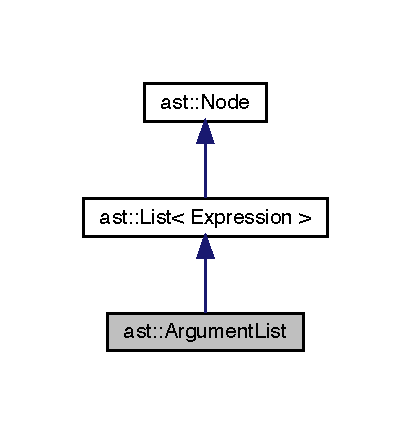
\includegraphics[width=197pt]{structast_1_1_argument_list__inherit__graph}
\end{center}
\end{figure}


Collaboration diagram for ast\+:\+:Argument\+List\+:
\nopagebreak
\begin{figure}[H]
\begin{center}
\leavevmode
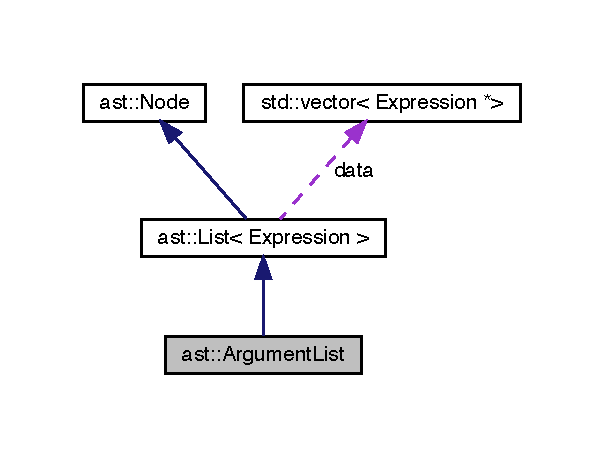
\includegraphics[width=290pt]{structast_1_1_argument_list__coll__graph}
\end{center}
\end{figure}
\subsection*{Public Member Functions}
\begin{DoxyCompactItemize}
\item 
{\footnotesize template$<$typename... Args$>$ }\\\hyperlink{structast_1_1_argument_list_a88c8ac45de2ea2f210d272ea898f26c2}{Argument\+List} (Args \&\&... args)
\end{DoxyCompactItemize}
\subsection*{Additional Inherited Members}


\subsection{Constructor \& Destructor Documentation}
\mbox{\Hypertarget{structast_1_1_argument_list_a88c8ac45de2ea2f210d272ea898f26c2}\label{structast_1_1_argument_list_a88c8ac45de2ea2f210d272ea898f26c2}} 
\index{ast\+::\+Argument\+List@{ast\+::\+Argument\+List}!Argument\+List@{Argument\+List}}
\index{Argument\+List@{Argument\+List}!ast\+::\+Argument\+List@{ast\+::\+Argument\+List}}
\subsubsection{\texorpdfstring{Argument\+List()}{ArgumentList()}}
{\footnotesize\ttfamily template$<$typename... Args$>$ \\
ast\+::\+Argument\+List\+::\+Argument\+List (\begin{DoxyParamCaption}\item[{Args \&\&...}]{args }\end{DoxyParamCaption})\hspace{0.3cm}{\ttfamily [inline]}}



The documentation for this struct was generated from the following file\+:\begin{DoxyCompactItemize}
\item 
src/\hyperlink{ast_8h}{ast.\+h}\end{DoxyCompactItemize}

\hypertarget{structast_1_1_arguments}{}\section{ast\+:\+:Arguments Struct Reference}
\label{structast_1_1_arguments}\index{ast\+::\+Arguments@{ast\+::\+Arguments}}


{\ttfamily \#include $<$ast.\+h$>$}



Inheritance diagram for ast\+:\+:Arguments\+:\nopagebreak
\begin{figure}[H]
\begin{center}
\leavevmode
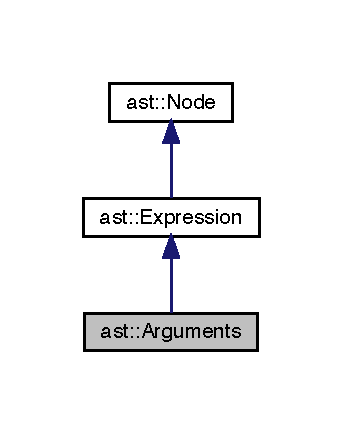
\includegraphics[width=164pt]{structast_1_1_arguments__inherit__graph}
\end{center}
\end{figure}


Collaboration diagram for ast\+:\+:Arguments\+:\nopagebreak
\begin{figure}[H]
\begin{center}
\leavevmode
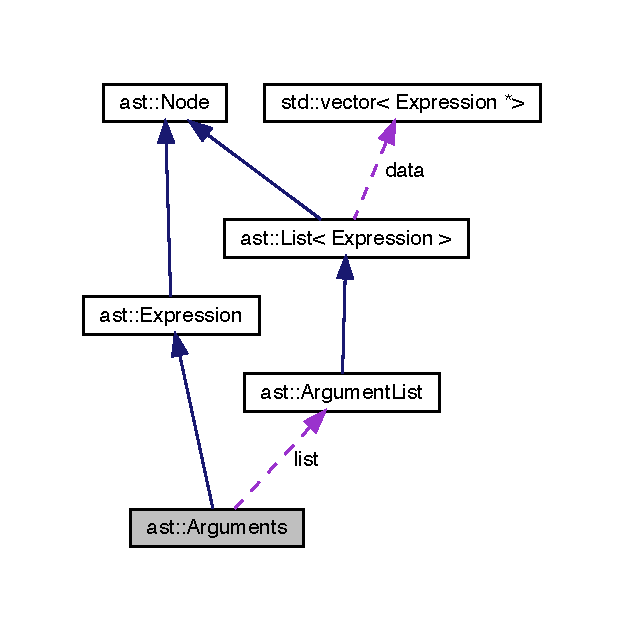
\includegraphics[width=300pt]{structast_1_1_arguments__coll__graph}
\end{center}
\end{figure}
\subsection*{Public Member Functions}
\begin{DoxyCompactItemize}
\item 
\hyperlink{structast_1_1_arguments_a3b7b4129f023820800c4c868b4dde923}{Arguments} (\hyperlink{structast_1_1_argument_list}{Argument\+List} $\ast$\hyperlink{structast_1_1_arguments_ab37e8d216047d6b1cdbc7eee2b1bb2db}{list}=nullptr)
\item 
void \hyperlink{structast_1_1_arguments_a85dac892bff5ef780b46c3683868cdde}{accept} (\hyperlink{structast_1_1_visitor}{Visitor} \&visitor) const override
\end{DoxyCompactItemize}
\subsection*{Public Attributes}
\begin{DoxyCompactItemize}
\item 
\hyperlink{structast_1_1_argument_list}{Argument\+List} $\ast$ \hyperlink{structast_1_1_arguments_ab37e8d216047d6b1cdbc7eee2b1bb2db}{list}
\end{DoxyCompactItemize}


\subsection{Constructor \& Destructor Documentation}
\mbox{\Hypertarget{structast_1_1_arguments_a3b7b4129f023820800c4c868b4dde923}\label{structast_1_1_arguments_a3b7b4129f023820800c4c868b4dde923}} 
\index{ast\+::\+Arguments@{ast\+::\+Arguments}!Arguments@{Arguments}}
\index{Arguments@{Arguments}!ast\+::\+Arguments@{ast\+::\+Arguments}}
\subsubsection{\texorpdfstring{Arguments()}{Arguments()}}
{\footnotesize\ttfamily ast\+::\+Arguments\+::\+Arguments (\begin{DoxyParamCaption}\item[{\hyperlink{structast_1_1_argument_list}{Argument\+List} $\ast$}]{list = {\ttfamily nullptr} }\end{DoxyParamCaption})\hspace{0.3cm}{\ttfamily [inline]}}



\subsection{Member Function Documentation}
\mbox{\Hypertarget{structast_1_1_arguments_a85dac892bff5ef780b46c3683868cdde}\label{structast_1_1_arguments_a85dac892bff5ef780b46c3683868cdde}} 
\index{ast\+::\+Arguments@{ast\+::\+Arguments}!accept@{accept}}
\index{accept@{accept}!ast\+::\+Arguments@{ast\+::\+Arguments}}
\subsubsection{\texorpdfstring{accept()}{accept()}}
{\footnotesize\ttfamily void ast\+::\+Arguments\+::accept (\begin{DoxyParamCaption}\item[{\hyperlink{structast_1_1_visitor}{Visitor} \&}]{visitor }\end{DoxyParamCaption}) const\hspace{0.3cm}{\ttfamily [inline]}, {\ttfamily [override]}, {\ttfamily [virtual]}}



Implements \hyperlink{structast_1_1_node_abc089ee6caaf06a4445ebdd8391fdebc}{ast\+::\+Node}.



\subsection{Member Data Documentation}
\mbox{\Hypertarget{structast_1_1_arguments_ab37e8d216047d6b1cdbc7eee2b1bb2db}\label{structast_1_1_arguments_ab37e8d216047d6b1cdbc7eee2b1bb2db}} 
\index{ast\+::\+Arguments@{ast\+::\+Arguments}!list@{list}}
\index{list@{list}!ast\+::\+Arguments@{ast\+::\+Arguments}}
\subsubsection{\texorpdfstring{list}{list}}
{\footnotesize\ttfamily \hyperlink{structast_1_1_argument_list}{Argument\+List}$\ast$ ast\+::\+Arguments\+::list}



The documentation for this struct was generated from the following file\+:\begin{DoxyCompactItemize}
\item 
src/\hyperlink{ast_8h}{ast.\+h}\end{DoxyCompactItemize}

\hypertarget{structast_1_1_array_literal}{}\section{ast\+:\+:Array\+Literal Struct Reference}
\label{structast_1_1_array_literal}\index{ast\+::\+Array\+Literal@{ast\+::\+Array\+Literal}}


{\ttfamily \#include $<$ast.\+h$>$}



Inheritance diagram for ast\+:\+:Array\+Literal\+:
\nopagebreak
\begin{figure}[H]
\begin{center}
\leavevmode
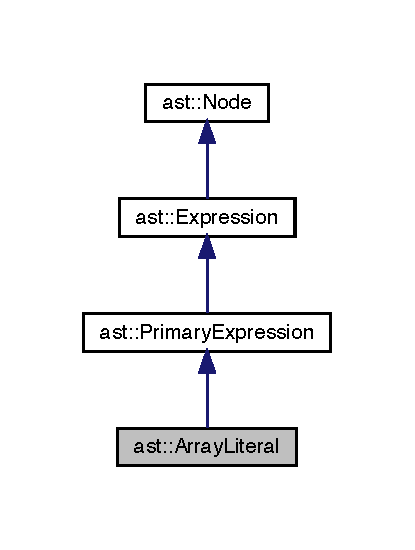
\includegraphics[width=199pt]{structast_1_1_array_literal__inherit__graph}
\end{center}
\end{figure}


Collaboration diagram for ast\+:\+:Array\+Literal\+:
\nopagebreak
\begin{figure}[H]
\begin{center}
\leavevmode
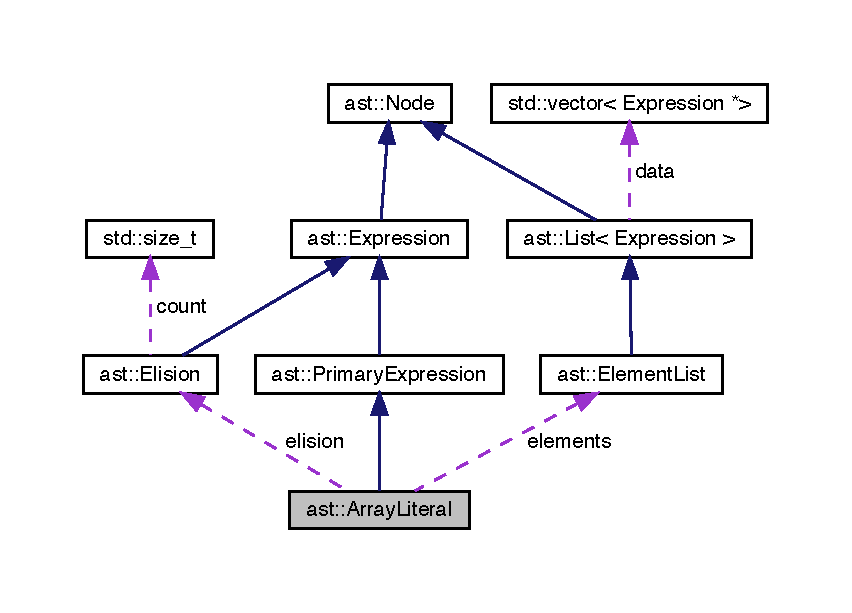
\includegraphics[width=350pt]{structast_1_1_array_literal__coll__graph}
\end{center}
\end{figure}
\subsection*{Public Member Functions}
\begin{DoxyCompactItemize}
\item 
\hyperlink{structast_1_1_array_literal_afee8504dca1587e8e0f9df5dd7a5ad05}{Array\+Literal} (\hyperlink{structast_1_1_element_list}{Element\+List} $\ast$\hyperlink{structast_1_1_array_literal_a3654b169349b3d309f65da79158dad56}{elements}=nullptr, \hyperlink{structast_1_1_elision}{Elision} $\ast$\hyperlink{structast_1_1_array_literal_ab6c8555816219a172d2b5c44dcbcf8d2}{elision}=nullptr)
\item 
void \hyperlink{structast_1_1_array_literal_a1efd88bd53842200c4b11d8afc17042f}{accept} (\hyperlink{structast_1_1_visitor}{Visitor} \&visitor) const override
\end{DoxyCompactItemize}
\subsection*{Public Attributes}
\begin{DoxyCompactItemize}
\item 
\hyperlink{structast_1_1_element_list}{Element\+List} $\ast$ \hyperlink{structast_1_1_array_literal_a3654b169349b3d309f65da79158dad56}{elements}
\item 
\hyperlink{structast_1_1_elision}{Elision} $\ast$ \hyperlink{structast_1_1_array_literal_ab6c8555816219a172d2b5c44dcbcf8d2}{elision}
\end{DoxyCompactItemize}


\subsection{Constructor \& Destructor Documentation}
\mbox{\Hypertarget{structast_1_1_array_literal_afee8504dca1587e8e0f9df5dd7a5ad05}\label{structast_1_1_array_literal_afee8504dca1587e8e0f9df5dd7a5ad05}} 
\index{ast\+::\+Array\+Literal@{ast\+::\+Array\+Literal}!Array\+Literal@{Array\+Literal}}
\index{Array\+Literal@{Array\+Literal}!ast\+::\+Array\+Literal@{ast\+::\+Array\+Literal}}
\subsubsection{\texorpdfstring{Array\+Literal()}{ArrayLiteral()}}
{\footnotesize\ttfamily ast\+::\+Array\+Literal\+::\+Array\+Literal (\begin{DoxyParamCaption}\item[{\hyperlink{structast_1_1_element_list}{Element\+List} $\ast$}]{elements = {\ttfamily nullptr},  }\item[{\hyperlink{structast_1_1_elision}{Elision} $\ast$}]{elision = {\ttfamily nullptr} }\end{DoxyParamCaption})\hspace{0.3cm}{\ttfamily [inline]}}



\subsection{Member Function Documentation}
\mbox{\Hypertarget{structast_1_1_array_literal_a1efd88bd53842200c4b11d8afc17042f}\label{structast_1_1_array_literal_a1efd88bd53842200c4b11d8afc17042f}} 
\index{ast\+::\+Array\+Literal@{ast\+::\+Array\+Literal}!accept@{accept}}
\index{accept@{accept}!ast\+::\+Array\+Literal@{ast\+::\+Array\+Literal}}
\subsubsection{\texorpdfstring{accept()}{accept()}}
{\footnotesize\ttfamily void ast\+::\+Array\+Literal\+::accept (\begin{DoxyParamCaption}\item[{\hyperlink{structast_1_1_visitor}{Visitor} \&}]{visitor }\end{DoxyParamCaption}) const\hspace{0.3cm}{\ttfamily [inline]}, {\ttfamily [override]}, {\ttfamily [virtual]}}



Implements \hyperlink{structast_1_1_node_abc089ee6caaf06a4445ebdd8391fdebc}{ast\+::\+Node}.



\subsection{Member Data Documentation}
\mbox{\Hypertarget{structast_1_1_array_literal_a3654b169349b3d309f65da79158dad56}\label{structast_1_1_array_literal_a3654b169349b3d309f65da79158dad56}} 
\index{ast\+::\+Array\+Literal@{ast\+::\+Array\+Literal}!elements@{elements}}
\index{elements@{elements}!ast\+::\+Array\+Literal@{ast\+::\+Array\+Literal}}
\subsubsection{\texorpdfstring{elements}{elements}}
{\footnotesize\ttfamily \hyperlink{structast_1_1_element_list}{Element\+List}$\ast$ ast\+::\+Array\+Literal\+::elements}

\mbox{\Hypertarget{structast_1_1_array_literal_ab6c8555816219a172d2b5c44dcbcf8d2}\label{structast_1_1_array_literal_ab6c8555816219a172d2b5c44dcbcf8d2}} 
\index{ast\+::\+Array\+Literal@{ast\+::\+Array\+Literal}!elision@{elision}}
\index{elision@{elision}!ast\+::\+Array\+Literal@{ast\+::\+Array\+Literal}}
\subsubsection{\texorpdfstring{elision}{elision}}
{\footnotesize\ttfamily \hyperlink{structast_1_1_elision}{Elision}$\ast$ ast\+::\+Array\+Literal\+::elision}



The documentation for this struct was generated from the following file\+:\begin{DoxyCompactItemize}
\item 
src/\hyperlink{ast_8h}{ast.\+h}\end{DoxyCompactItemize}

\hypertarget{class_basic_lexer}{}\section{Basic\+Lexer$<$ T $>$ Class Template Reference}
\label{class_basic_lexer}\index{Basic\+Lexer$<$ T $>$@{Basic\+Lexer$<$ T $>$}}


{\ttfamily \#include $<$lexer.\+h$>$}



Inheritance diagram for Basic\+Lexer$<$ T $>$\+:\nopagebreak
\begin{figure}[H]
\begin{center}
\leavevmode
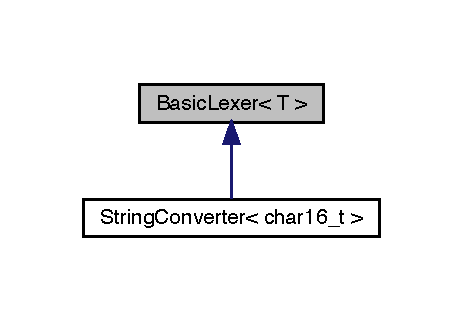
\includegraphics[width=222pt]{class_basic_lexer__inherit__graph}
\end{center}
\end{figure}
\subsection*{Public Member Functions}
\begin{DoxyCompactItemize}
\item 
\hyperlink{class_basic_lexer_abc267aed0ef7227486b932f13b2917f0}{Basic\+Lexer} ()
\item 
\hyperlink{class_basic_lexer_a58d2038fb47025d4e32c20750e713b43}{Basic\+Lexer} (\textbf{ std\+::initializer\+\_\+list}$<$ \hyperlink{class_token}{Token} $>$ \hyperlink{class_basic_lexer_ac20fdf19d5602c563b5cad2bae3ad803}{tokens})
\item 
\hyperlink{class_basic_lexer_a1fd5d2795464497ffbe2bf61c892d619}{Basic\+Lexer} (\textbf{ std\+::vector}$<$ \hyperlink{class_token}{Token} $>$ \hyperlink{class_basic_lexer_ac20fdf19d5602c563b5cad2bae3ad803}{tokens})
\item 
{\footnotesize template$<$typename It $>$ }\\\hyperlink{class_basic_lexer_a7b8cb3ec8ba1ef5567bd280800f891f8}{Basic\+Lexer} (It begin, It end)
\item 
\hyperlink{class_basic_lexer_aee8242905dd2c3541322900bdd05a7b7}{Basic\+Lexer} (const \textbf{ std\+::u16string} \&str)
\item 
\hyperlink{class_basic_lexer_ab486a96453887dc7f9efd08c518ae0b0}{Basic\+Lexer} (const \textbf{ std\+::string} \&str)
\item 
Tokens \hyperlink{class_basic_lexer_ac20fdf19d5602c563b5cad2bae3ad803}{tokens} () const
\end{DoxyCompactItemize}


\subsection{Constructor \& Destructor Documentation}
\mbox{\Hypertarget{class_basic_lexer_abc267aed0ef7227486b932f13b2917f0}\label{class_basic_lexer_abc267aed0ef7227486b932f13b2917f0}} 
\index{Basic\+Lexer@{Basic\+Lexer}!Basic\+Lexer@{Basic\+Lexer}}
\index{Basic\+Lexer@{Basic\+Lexer}!Basic\+Lexer@{Basic\+Lexer}}
\subsubsection{\texorpdfstring{Basic\+Lexer()}{BasicLexer()}\hspace{0.1cm}{\footnotesize\ttfamily [1/6]}}
{\footnotesize\ttfamily template$<$typename T$>$ \\
\hyperlink{class_basic_lexer}{Basic\+Lexer}$<$ T $>$\+::\hyperlink{class_basic_lexer}{Basic\+Lexer} (\begin{DoxyParamCaption}{ }\end{DoxyParamCaption})\hspace{0.3cm}{\ttfamily [inline]}}

\mbox{\Hypertarget{class_basic_lexer_a58d2038fb47025d4e32c20750e713b43}\label{class_basic_lexer_a58d2038fb47025d4e32c20750e713b43}} 
\index{Basic\+Lexer@{Basic\+Lexer}!Basic\+Lexer@{Basic\+Lexer}}
\index{Basic\+Lexer@{Basic\+Lexer}!Basic\+Lexer@{Basic\+Lexer}}
\subsubsection{\texorpdfstring{Basic\+Lexer()}{BasicLexer()}\hspace{0.1cm}{\footnotesize\ttfamily [2/6]}}
{\footnotesize\ttfamily template$<$typename T$>$ \\
\hyperlink{class_basic_lexer}{Basic\+Lexer}$<$ T $>$\+::\hyperlink{class_basic_lexer}{Basic\+Lexer} (\begin{DoxyParamCaption}\item[{\textbf{ std\+::initializer\+\_\+list}$<$ \hyperlink{class_token}{Token} $>$}]{tokens }\end{DoxyParamCaption})\hspace{0.3cm}{\ttfamily [inline]}}

\mbox{\Hypertarget{class_basic_lexer_a1fd5d2795464497ffbe2bf61c892d619}\label{class_basic_lexer_a1fd5d2795464497ffbe2bf61c892d619}} 
\index{Basic\+Lexer@{Basic\+Lexer}!Basic\+Lexer@{Basic\+Lexer}}
\index{Basic\+Lexer@{Basic\+Lexer}!Basic\+Lexer@{Basic\+Lexer}}
\subsubsection{\texorpdfstring{Basic\+Lexer()}{BasicLexer()}\hspace{0.1cm}{\footnotesize\ttfamily [3/6]}}
{\footnotesize\ttfamily template$<$typename T$>$ \\
\hyperlink{class_basic_lexer}{Basic\+Lexer}$<$ T $>$\+::\hyperlink{class_basic_lexer}{Basic\+Lexer} (\begin{DoxyParamCaption}\item[{\textbf{ std\+::vector}$<$ \hyperlink{class_token}{Token} $>$}]{tokens }\end{DoxyParamCaption})\hspace{0.3cm}{\ttfamily [inline]}}

\mbox{\Hypertarget{class_basic_lexer_a7b8cb3ec8ba1ef5567bd280800f891f8}\label{class_basic_lexer_a7b8cb3ec8ba1ef5567bd280800f891f8}} 
\index{Basic\+Lexer@{Basic\+Lexer}!Basic\+Lexer@{Basic\+Lexer}}
\index{Basic\+Lexer@{Basic\+Lexer}!Basic\+Lexer@{Basic\+Lexer}}
\subsubsection{\texorpdfstring{Basic\+Lexer()}{BasicLexer()}\hspace{0.1cm}{\footnotesize\ttfamily [4/6]}}
{\footnotesize\ttfamily template$<$typename T$>$ \\
template$<$typename It $>$ \\
\hyperlink{class_basic_lexer}{Basic\+Lexer}$<$ T $>$\+::\hyperlink{class_basic_lexer}{Basic\+Lexer} (\begin{DoxyParamCaption}\item[{It}]{begin,  }\item[{It}]{end }\end{DoxyParamCaption})\hspace{0.3cm}{\ttfamily [inline]}}

\mbox{\Hypertarget{class_basic_lexer_aee8242905dd2c3541322900bdd05a7b7}\label{class_basic_lexer_aee8242905dd2c3541322900bdd05a7b7}} 
\index{Basic\+Lexer@{Basic\+Lexer}!Basic\+Lexer@{Basic\+Lexer}}
\index{Basic\+Lexer@{Basic\+Lexer}!Basic\+Lexer@{Basic\+Lexer}}
\subsubsection{\texorpdfstring{Basic\+Lexer()}{BasicLexer()}\hspace{0.1cm}{\footnotesize\ttfamily [5/6]}}
{\footnotesize\ttfamily template$<$typename T$>$ \\
\hyperlink{class_basic_lexer}{Basic\+Lexer}$<$ T $>$\+::\hyperlink{class_basic_lexer}{Basic\+Lexer} (\begin{DoxyParamCaption}\item[{const \textbf{ std\+::u16string} \&}]{str }\end{DoxyParamCaption})\hspace{0.3cm}{\ttfamily [inline]}}

\mbox{\Hypertarget{class_basic_lexer_ab486a96453887dc7f9efd08c518ae0b0}\label{class_basic_lexer_ab486a96453887dc7f9efd08c518ae0b0}} 
\index{Basic\+Lexer@{Basic\+Lexer}!Basic\+Lexer@{Basic\+Lexer}}
\index{Basic\+Lexer@{Basic\+Lexer}!Basic\+Lexer@{Basic\+Lexer}}
\subsubsection{\texorpdfstring{Basic\+Lexer()}{BasicLexer()}\hspace{0.1cm}{\footnotesize\ttfamily [6/6]}}
{\footnotesize\ttfamily template$<$typename T$>$ \\
\hyperlink{class_basic_lexer}{Basic\+Lexer}$<$ T $>$\+::\hyperlink{class_basic_lexer}{Basic\+Lexer} (\begin{DoxyParamCaption}\item[{const \textbf{ std\+::string} \&}]{str }\end{DoxyParamCaption})\hspace{0.3cm}{\ttfamily [inline]}}



\subsection{Member Function Documentation}
\mbox{\Hypertarget{class_basic_lexer_ac20fdf19d5602c563b5cad2bae3ad803}\label{class_basic_lexer_ac20fdf19d5602c563b5cad2bae3ad803}} 
\index{Basic\+Lexer@{Basic\+Lexer}!tokens@{tokens}}
\index{tokens@{tokens}!Basic\+Lexer@{Basic\+Lexer}}
\subsubsection{\texorpdfstring{tokens()}{tokens()}}
{\footnotesize\ttfamily template$<$typename T$>$ \\
Tokens \hyperlink{class_basic_lexer}{Basic\+Lexer}$<$ T $>$\+::tokens (\begin{DoxyParamCaption}{ }\end{DoxyParamCaption}) const\hspace{0.3cm}{\ttfamily [inline]}}



The documentation for this class was generated from the following file\+:\begin{DoxyCompactItemize}
\item 
src/\hyperlink{lexer_8h}{lexer.\+h}\end{DoxyCompactItemize}

\hypertarget{structast_1_1_binary_expression}{}\section{ast\+:\+:Binary\+Expression Struct Reference}
\label{structast_1_1_binary_expression}\index{ast\+::\+Binary\+Expression@{ast\+::\+Binary\+Expression}}


{\ttfamily \#include $<$ast.\+h$>$}



Inheritance diagram for ast\+:\+:Binary\+Expression\+:\nopagebreak
\begin{figure}[H]
\begin{center}
\leavevmode
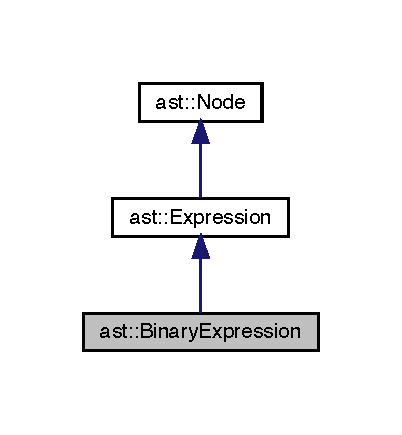
\includegraphics[width=193pt]{structast_1_1_binary_expression__inherit__graph}
\end{center}
\end{figure}


Collaboration diagram for ast\+:\+:Binary\+Expression\+:\nopagebreak
\begin{figure}[H]
\begin{center}
\leavevmode
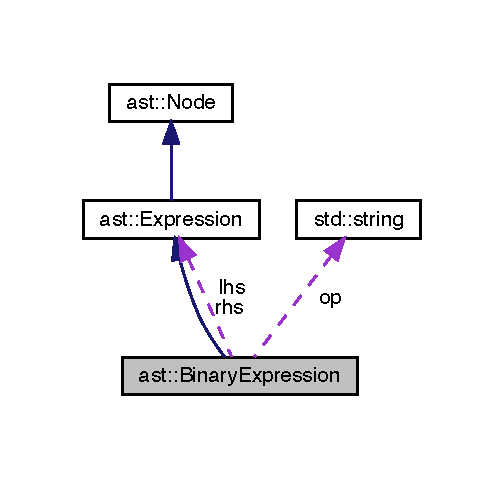
\includegraphics[width=242pt]{structast_1_1_binary_expression__coll__graph}
\end{center}
\end{figure}
\subsection*{Public Member Functions}
\begin{DoxyCompactItemize}
\item 
\hyperlink{structast_1_1_binary_expression_a07e1dc9e731ef1913deff32579929c8c}{Binary\+Expression} (\textbf{ std\+::string} \hyperlink{structast_1_1_binary_expression_a7621248e9b4f08d2987b86758a832801}{op}, \hyperlink{structast_1_1_expression}{Expression} $\ast$\hyperlink{structast_1_1_binary_expression_a1c8d523d75c0200e18b9511af135c292}{lhs}=nullptr, \hyperlink{structast_1_1_expression}{Expression} $\ast$\hyperlink{structast_1_1_binary_expression_a9f298035c5a0f9169ba7c10f2ce1722a}{rhs}=nullptr)
\item 
void \hyperlink{structast_1_1_binary_expression_ad962b349492ab7dc7365a5c6d7153d71}{accept} (\hyperlink{structast_1_1_visitor}{Visitor} \&visitor) const override
\end{DoxyCompactItemize}
\subsection*{Public Attributes}
\begin{DoxyCompactItemize}
\item 
\textbf{ std\+::string} \hyperlink{structast_1_1_binary_expression_a7621248e9b4f08d2987b86758a832801}{op}
\item 
\hyperlink{structast_1_1_expression}{Expression} $\ast$ \hyperlink{structast_1_1_binary_expression_a1c8d523d75c0200e18b9511af135c292}{lhs}
\item 
\hyperlink{structast_1_1_expression}{Expression} $\ast$ \hyperlink{structast_1_1_binary_expression_a9f298035c5a0f9169ba7c10f2ce1722a}{rhs}
\end{DoxyCompactItemize}


\subsection{Constructor \& Destructor Documentation}
\mbox{\Hypertarget{structast_1_1_binary_expression_a07e1dc9e731ef1913deff32579929c8c}\label{structast_1_1_binary_expression_a07e1dc9e731ef1913deff32579929c8c}} 
\index{ast\+::\+Binary\+Expression@{ast\+::\+Binary\+Expression}!Binary\+Expression@{Binary\+Expression}}
\index{Binary\+Expression@{Binary\+Expression}!ast\+::\+Binary\+Expression@{ast\+::\+Binary\+Expression}}
\subsubsection{\texorpdfstring{Binary\+Expression()}{BinaryExpression()}}
{\footnotesize\ttfamily ast\+::\+Binary\+Expression\+::\+Binary\+Expression (\begin{DoxyParamCaption}\item[{\textbf{ std\+::string}}]{op,  }\item[{\hyperlink{structast_1_1_expression}{Expression} $\ast$}]{lhs = {\ttfamily nullptr},  }\item[{\hyperlink{structast_1_1_expression}{Expression} $\ast$}]{rhs = {\ttfamily nullptr} }\end{DoxyParamCaption})\hspace{0.3cm}{\ttfamily [inline]}}



\subsection{Member Function Documentation}
\mbox{\Hypertarget{structast_1_1_binary_expression_ad962b349492ab7dc7365a5c6d7153d71}\label{structast_1_1_binary_expression_ad962b349492ab7dc7365a5c6d7153d71}} 
\index{ast\+::\+Binary\+Expression@{ast\+::\+Binary\+Expression}!accept@{accept}}
\index{accept@{accept}!ast\+::\+Binary\+Expression@{ast\+::\+Binary\+Expression}}
\subsubsection{\texorpdfstring{accept()}{accept()}}
{\footnotesize\ttfamily void ast\+::\+Binary\+Expression\+::accept (\begin{DoxyParamCaption}\item[{\hyperlink{structast_1_1_visitor}{Visitor} \&}]{visitor }\end{DoxyParamCaption}) const\hspace{0.3cm}{\ttfamily [inline]}, {\ttfamily [override]}, {\ttfamily [virtual]}}



Implements \hyperlink{structast_1_1_node_abc089ee6caaf06a4445ebdd8391fdebc}{ast\+::\+Node}.



\subsection{Member Data Documentation}
\mbox{\Hypertarget{structast_1_1_binary_expression_a1c8d523d75c0200e18b9511af135c292}\label{structast_1_1_binary_expression_a1c8d523d75c0200e18b9511af135c292}} 
\index{ast\+::\+Binary\+Expression@{ast\+::\+Binary\+Expression}!lhs@{lhs}}
\index{lhs@{lhs}!ast\+::\+Binary\+Expression@{ast\+::\+Binary\+Expression}}
\subsubsection{\texorpdfstring{lhs}{lhs}}
{\footnotesize\ttfamily \hyperlink{structast_1_1_expression}{Expression}$\ast$ ast\+::\+Binary\+Expression\+::lhs}

\mbox{\Hypertarget{structast_1_1_binary_expression_a7621248e9b4f08d2987b86758a832801}\label{structast_1_1_binary_expression_a7621248e9b4f08d2987b86758a832801}} 
\index{ast\+::\+Binary\+Expression@{ast\+::\+Binary\+Expression}!op@{op}}
\index{op@{op}!ast\+::\+Binary\+Expression@{ast\+::\+Binary\+Expression}}
\subsubsection{\texorpdfstring{op}{op}}
{\footnotesize\ttfamily \textbf{ std\+::string} ast\+::\+Binary\+Expression\+::op}

\mbox{\Hypertarget{structast_1_1_binary_expression_a9f298035c5a0f9169ba7c10f2ce1722a}\label{structast_1_1_binary_expression_a9f298035c5a0f9169ba7c10f2ce1722a}} 
\index{ast\+::\+Binary\+Expression@{ast\+::\+Binary\+Expression}!rhs@{rhs}}
\index{rhs@{rhs}!ast\+::\+Binary\+Expression@{ast\+::\+Binary\+Expression}}
\subsubsection{\texorpdfstring{rhs}{rhs}}
{\footnotesize\ttfamily \hyperlink{structast_1_1_expression}{Expression}$\ast$ ast\+::\+Binary\+Expression\+::rhs}



The documentation for this struct was generated from the following file\+:\begin{DoxyCompactItemize}
\item 
src/\hyperlink{ast_8h}{ast.\+h}\end{DoxyCompactItemize}

\hypertarget{structast_1_1_block}{}\section{ast\+:\+:Block Struct Reference}
\label{structast_1_1_block}\index{ast\+::\+Block@{ast\+::\+Block}}


{\ttfamily \#include $<$ast.\+h$>$}



Inheritance diagram for ast\+:\+:Block\+:
\nopagebreak
\begin{figure}[H]
\begin{center}
\leavevmode
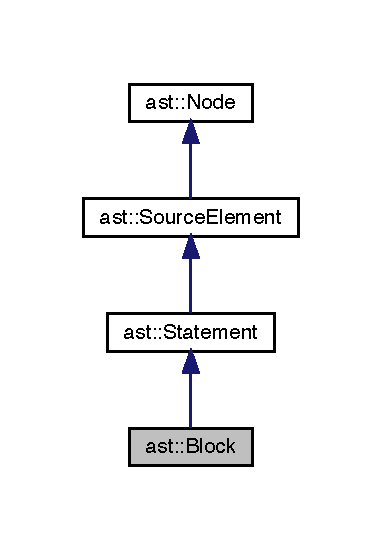
\includegraphics[width=183pt]{structast_1_1_block__inherit__graph}
\end{center}
\end{figure}


Collaboration diagram for ast\+:\+:Block\+:
\nopagebreak
\begin{figure}[H]
\begin{center}
\leavevmode
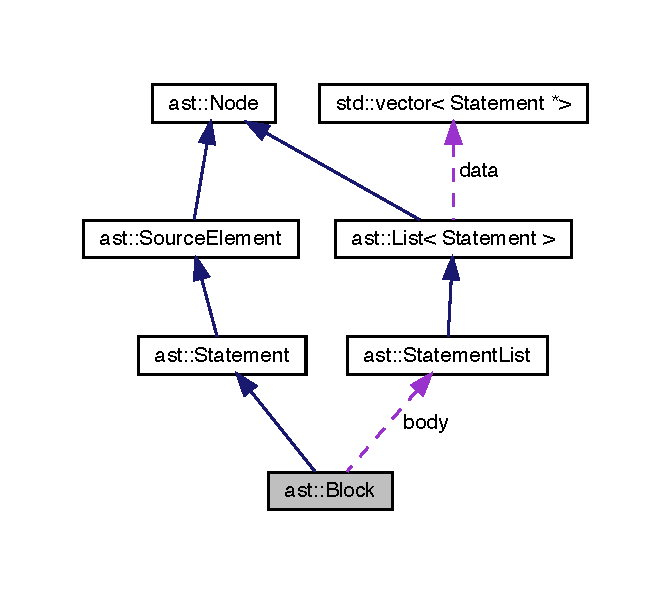
\includegraphics[width=322pt]{structast_1_1_block__coll__graph}
\end{center}
\end{figure}
\subsection*{Public Member Functions}
\begin{DoxyCompactItemize}
\item 
\hyperlink{structast_1_1_block_a006d000dd65024c61c84bf0b956b5f6e}{Block} (\hyperlink{structast_1_1_statement_list}{Statement\+List} $\ast$\hyperlink{structast_1_1_block_a7d7ba772aed3b8db5e26360b4f613410}{body}=nullptr)
\item 
void \hyperlink{structast_1_1_block_a8aec4a97d7f490096ea39ccac79c8676}{accept} (\hyperlink{structast_1_1_visitor}{Visitor} \&visitor) const override
\end{DoxyCompactItemize}
\subsection*{Public Attributes}
\begin{DoxyCompactItemize}
\item 
\hyperlink{structast_1_1_statement_list}{Statement\+List} $\ast$ \hyperlink{structast_1_1_block_a7d7ba772aed3b8db5e26360b4f613410}{body}
\end{DoxyCompactItemize}


\subsection{Constructor \& Destructor Documentation}
\mbox{\Hypertarget{structast_1_1_block_a006d000dd65024c61c84bf0b956b5f6e}\label{structast_1_1_block_a006d000dd65024c61c84bf0b956b5f6e}} 
\index{ast\+::\+Block@{ast\+::\+Block}!Block@{Block}}
\index{Block@{Block}!ast\+::\+Block@{ast\+::\+Block}}
\subsubsection{\texorpdfstring{Block()}{Block()}}
{\footnotesize\ttfamily ast\+::\+Block\+::\+Block (\begin{DoxyParamCaption}\item[{\hyperlink{structast_1_1_statement_list}{Statement\+List} $\ast$}]{body = {\ttfamily nullptr} }\end{DoxyParamCaption})\hspace{0.3cm}{\ttfamily [inline]}}



\subsection{Member Function Documentation}
\mbox{\Hypertarget{structast_1_1_block_a8aec4a97d7f490096ea39ccac79c8676}\label{structast_1_1_block_a8aec4a97d7f490096ea39ccac79c8676}} 
\index{ast\+::\+Block@{ast\+::\+Block}!accept@{accept}}
\index{accept@{accept}!ast\+::\+Block@{ast\+::\+Block}}
\subsubsection{\texorpdfstring{accept()}{accept()}}
{\footnotesize\ttfamily void ast\+::\+Block\+::accept (\begin{DoxyParamCaption}\item[{\hyperlink{structast_1_1_visitor}{Visitor} \&}]{visitor }\end{DoxyParamCaption}) const\hspace{0.3cm}{\ttfamily [inline]}, {\ttfamily [override]}, {\ttfamily [virtual]}}



Implements \hyperlink{structast_1_1_node_abc089ee6caaf06a4445ebdd8391fdebc}{ast\+::\+Node}.



\subsection{Member Data Documentation}
\mbox{\Hypertarget{structast_1_1_block_a7d7ba772aed3b8db5e26360b4f613410}\label{structast_1_1_block_a7d7ba772aed3b8db5e26360b4f613410}} 
\index{ast\+::\+Block@{ast\+::\+Block}!body@{body}}
\index{body@{body}!ast\+::\+Block@{ast\+::\+Block}}
\subsubsection{\texorpdfstring{body}{body}}
{\footnotesize\ttfamily \hyperlink{structast_1_1_statement_list}{Statement\+List}$\ast$ ast\+::\+Block\+::body}



The documentation for this struct was generated from the following file\+:\begin{DoxyCompactItemize}
\item 
src/\hyperlink{ast_8h}{ast.\+h}\end{DoxyCompactItemize}

\hypertarget{struct_boolean}{}\section{Boolean Struct Reference}
\label{struct_boolean}\index{Boolean@{Boolean}}


{\ttfamily \#include $<$value.\+h$>$}

\subsection*{Public Attributes}
\begin{DoxyCompactItemize}
\item 
bool \hyperlink{struct_boolean_a8e44c7f95d984f2dc8c6974f607b2b36}{value}
\end{DoxyCompactItemize}


\subsection{Member Data Documentation}
\mbox{\Hypertarget{struct_boolean_a8e44c7f95d984f2dc8c6974f607b2b36}\label{struct_boolean_a8e44c7f95d984f2dc8c6974f607b2b36}} 
\index{Boolean@{Boolean}!value@{value}}
\index{value@{value}!Boolean@{Boolean}}
\subsubsection{\texorpdfstring{value}{value}}
{\footnotesize\ttfamily bool Boolean\+::value}



The documentation for this struct was generated from the following file\+:\begin{DoxyCompactItemize}
\item 
src/\hyperlink{value_8h}{value.\+h}\end{DoxyCompactItemize}

\hypertarget{structast_1_1_boolean_literal}{}\section{ast\+:\+:Boolean\+Literal Struct Reference}
\label{structast_1_1_boolean_literal}\index{ast\+::\+Boolean\+Literal@{ast\+::\+Boolean\+Literal}}


{\ttfamily \#include $<$ast.\+h$>$}



Inheritance diagram for ast\+:\+:Boolean\+Literal\+:
\nopagebreak
\begin{figure}[H]
\begin{center}
\leavevmode
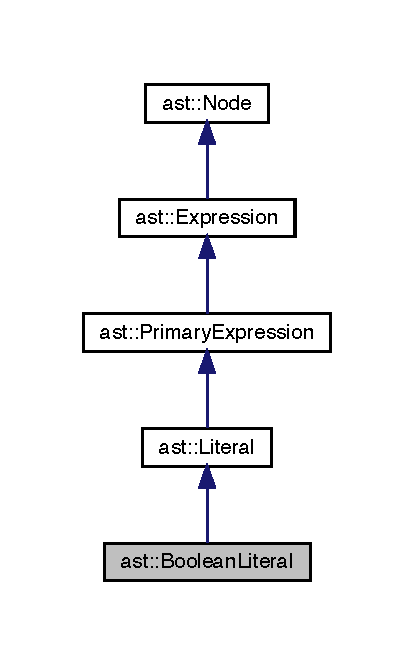
\includegraphics[width=179pt]{structast_1_1_boolean_literal__inherit__graph}
\end{center}
\end{figure}


Collaboration diagram for ast\+:\+:Boolean\+Literal\+:
\nopagebreak
\begin{figure}[H]
\begin{center}
\leavevmode
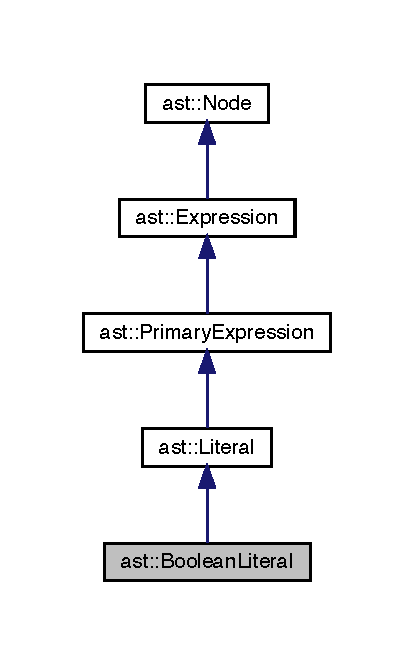
\includegraphics[width=179pt]{structast_1_1_boolean_literal__coll__graph}
\end{center}
\end{figure}
\subsection*{Public Member Functions}
\begin{DoxyCompactItemize}
\item 
\hyperlink{structast_1_1_boolean_literal_a3b8e0e317c0e0ec4baf49d677d1a5ec7}{Boolean\+Literal} (bool \hyperlink{structast_1_1_boolean_literal_a439b71339c83768f2bc892f5af84c540}{value})
\item 
void \hyperlink{structast_1_1_boolean_literal_a97e132542a670b2d893b46bd2c8b6217}{accept} (\hyperlink{structast_1_1_visitor}{Visitor} \&visitor) const override
\end{DoxyCompactItemize}
\subsection*{Public Attributes}
\begin{DoxyCompactItemize}
\item 
bool \hyperlink{structast_1_1_boolean_literal_a439b71339c83768f2bc892f5af84c540}{value}
\end{DoxyCompactItemize}


\subsection{Constructor \& Destructor Documentation}
\mbox{\Hypertarget{structast_1_1_boolean_literal_a3b8e0e317c0e0ec4baf49d677d1a5ec7}\label{structast_1_1_boolean_literal_a3b8e0e317c0e0ec4baf49d677d1a5ec7}} 
\index{ast\+::\+Boolean\+Literal@{ast\+::\+Boolean\+Literal}!Boolean\+Literal@{Boolean\+Literal}}
\index{Boolean\+Literal@{Boolean\+Literal}!ast\+::\+Boolean\+Literal@{ast\+::\+Boolean\+Literal}}
\subsubsection{\texorpdfstring{Boolean\+Literal()}{BooleanLiteral()}}
{\footnotesize\ttfamily ast\+::\+Boolean\+Literal\+::\+Boolean\+Literal (\begin{DoxyParamCaption}\item[{bool}]{value }\end{DoxyParamCaption})\hspace{0.3cm}{\ttfamily [inline]}}



\subsection{Member Function Documentation}
\mbox{\Hypertarget{structast_1_1_boolean_literal_a97e132542a670b2d893b46bd2c8b6217}\label{structast_1_1_boolean_literal_a97e132542a670b2d893b46bd2c8b6217}} 
\index{ast\+::\+Boolean\+Literal@{ast\+::\+Boolean\+Literal}!accept@{accept}}
\index{accept@{accept}!ast\+::\+Boolean\+Literal@{ast\+::\+Boolean\+Literal}}
\subsubsection{\texorpdfstring{accept()}{accept()}}
{\footnotesize\ttfamily void ast\+::\+Boolean\+Literal\+::accept (\begin{DoxyParamCaption}\item[{\hyperlink{structast_1_1_visitor}{Visitor} \&}]{visitor }\end{DoxyParamCaption}) const\hspace{0.3cm}{\ttfamily [inline]}, {\ttfamily [override]}, {\ttfamily [virtual]}}



Implements \hyperlink{structast_1_1_node_abc089ee6caaf06a4445ebdd8391fdebc}{ast\+::\+Node}.



\subsection{Member Data Documentation}
\mbox{\Hypertarget{structast_1_1_boolean_literal_a439b71339c83768f2bc892f5af84c540}\label{structast_1_1_boolean_literal_a439b71339c83768f2bc892f5af84c540}} 
\index{ast\+::\+Boolean\+Literal@{ast\+::\+Boolean\+Literal}!value@{value}}
\index{value@{value}!ast\+::\+Boolean\+Literal@{ast\+::\+Boolean\+Literal}}
\subsubsection{\texorpdfstring{value}{value}}
{\footnotesize\ttfamily bool ast\+::\+Boolean\+Literal\+::value}



The documentation for this struct was generated from the following file\+:\begin{DoxyCompactItemize}
\item 
src/\hyperlink{ast_8h}{ast.\+h}\end{DoxyCompactItemize}

\hypertarget{structast_1_1_break_statement}{}\section{ast\+:\+:Break\+Statement Struct Reference}
\label{structast_1_1_break_statement}\index{ast\+::\+Break\+Statement@{ast\+::\+Break\+Statement}}


{\ttfamily \#include $<$ast.\+h$>$}



Inheritance diagram for ast\+:\+:Break\+Statement\+:\nopagebreak
\begin{figure}[H]
\begin{center}
\leavevmode
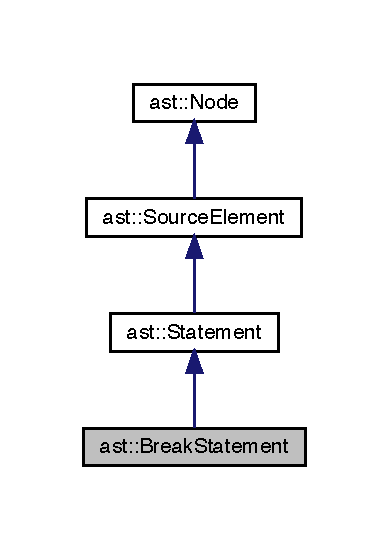
\includegraphics[width=187pt]{structast_1_1_break_statement__inherit__graph}
\end{center}
\end{figure}


Collaboration diagram for ast\+:\+:Break\+Statement\+:\nopagebreak
\begin{figure}[H]
\begin{center}
\leavevmode
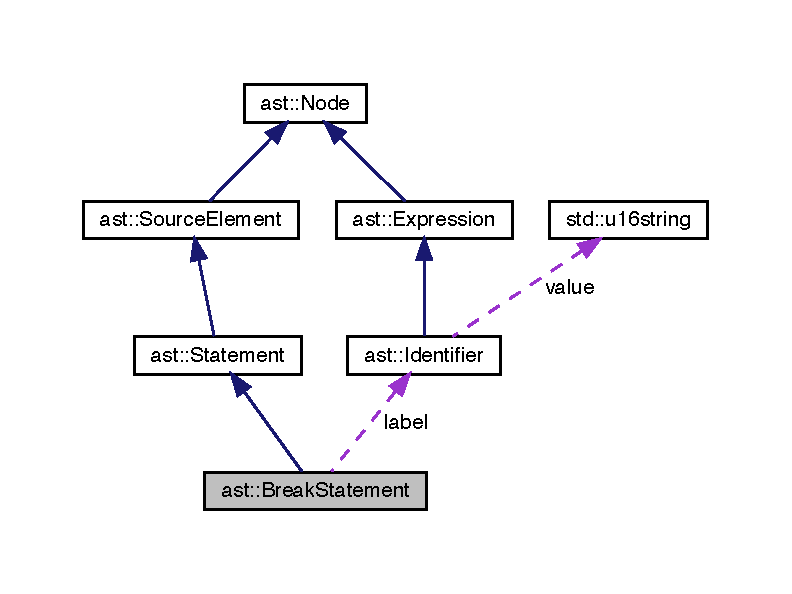
\includegraphics[width=350pt]{structast_1_1_break_statement__coll__graph}
\end{center}
\end{figure}
\subsection*{Public Member Functions}
\begin{DoxyCompactItemize}
\item 
\hyperlink{structast_1_1_break_statement_a9b8f2fabc03702b03f0b7b61c94f5189}{Break\+Statement} (\hyperlink{structast_1_1_identifier}{Identifier} $\ast$\hyperlink{structast_1_1_break_statement_ad38ca9b59202df6aad6e4ab09fc8316d}{label}=nullptr)
\item 
void \hyperlink{structast_1_1_break_statement_ac7db635ee58478c5f917a85bd7c70b79}{accept} (\hyperlink{structast_1_1_visitor}{Visitor} \&visitor) const override
\end{DoxyCompactItemize}
\subsection*{Public Attributes}
\begin{DoxyCompactItemize}
\item 
\hyperlink{structast_1_1_identifier}{Identifier} $\ast$ \hyperlink{structast_1_1_break_statement_ad38ca9b59202df6aad6e4ab09fc8316d}{label}
\end{DoxyCompactItemize}


\subsection{Constructor \& Destructor Documentation}
\mbox{\Hypertarget{structast_1_1_break_statement_a9b8f2fabc03702b03f0b7b61c94f5189}\label{structast_1_1_break_statement_a9b8f2fabc03702b03f0b7b61c94f5189}} 
\index{ast\+::\+Break\+Statement@{ast\+::\+Break\+Statement}!Break\+Statement@{Break\+Statement}}
\index{Break\+Statement@{Break\+Statement}!ast\+::\+Break\+Statement@{ast\+::\+Break\+Statement}}
\subsubsection{\texorpdfstring{Break\+Statement()}{BreakStatement()}}
{\footnotesize\ttfamily ast\+::\+Break\+Statement\+::\+Break\+Statement (\begin{DoxyParamCaption}\item[{\hyperlink{structast_1_1_identifier}{Identifier} $\ast$}]{label = {\ttfamily nullptr} }\end{DoxyParamCaption})\hspace{0.3cm}{\ttfamily [inline]}}



\subsection{Member Function Documentation}
\mbox{\Hypertarget{structast_1_1_break_statement_ac7db635ee58478c5f917a85bd7c70b79}\label{structast_1_1_break_statement_ac7db635ee58478c5f917a85bd7c70b79}} 
\index{ast\+::\+Break\+Statement@{ast\+::\+Break\+Statement}!accept@{accept}}
\index{accept@{accept}!ast\+::\+Break\+Statement@{ast\+::\+Break\+Statement}}
\subsubsection{\texorpdfstring{accept()}{accept()}}
{\footnotesize\ttfamily void ast\+::\+Break\+Statement\+::accept (\begin{DoxyParamCaption}\item[{\hyperlink{structast_1_1_visitor}{Visitor} \&}]{visitor }\end{DoxyParamCaption}) const\hspace{0.3cm}{\ttfamily [inline]}, {\ttfamily [override]}, {\ttfamily [virtual]}}



Implements \hyperlink{structast_1_1_node_abc089ee6caaf06a4445ebdd8391fdebc}{ast\+::\+Node}.



\subsection{Member Data Documentation}
\mbox{\Hypertarget{structast_1_1_break_statement_ad38ca9b59202df6aad6e4ab09fc8316d}\label{structast_1_1_break_statement_ad38ca9b59202df6aad6e4ab09fc8316d}} 
\index{ast\+::\+Break\+Statement@{ast\+::\+Break\+Statement}!label@{label}}
\index{label@{label}!ast\+::\+Break\+Statement@{ast\+::\+Break\+Statement}}
\subsubsection{\texorpdfstring{label}{label}}
{\footnotesize\ttfamily \hyperlink{structast_1_1_identifier}{Identifier}$\ast$ ast\+::\+Break\+Statement\+::label}



The documentation for this struct was generated from the following file\+:\begin{DoxyCompactItemize}
\item 
src/\hyperlink{ast_8h}{ast.\+h}\end{DoxyCompactItemize}

\hypertarget{struct_callable_visitor}{}\section{Callable\+Visitor$<$ Callable $>$ Struct Template Reference}
\label{struct_callable_visitor}\index{Callable\+Visitor$<$ Callable $>$@{Callable\+Visitor$<$ Callable $>$}}


Inheritance diagram for Callable\+Visitor$<$ Callable $>$\+:\nopagebreak
\begin{figure}[H]
\begin{center}
\leavevmode
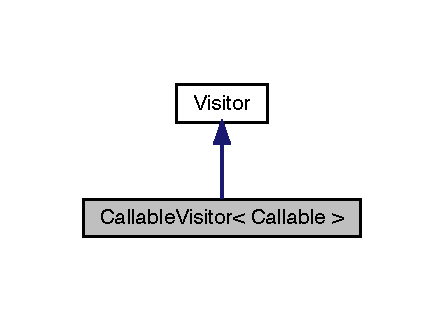
\includegraphics[width=213pt]{struct_callable_visitor__inherit__graph}
\end{center}
\end{figure}


Collaboration diagram for Callable\+Visitor$<$ Callable $>$\+:\nopagebreak
\begin{figure}[H]
\begin{center}
\leavevmode
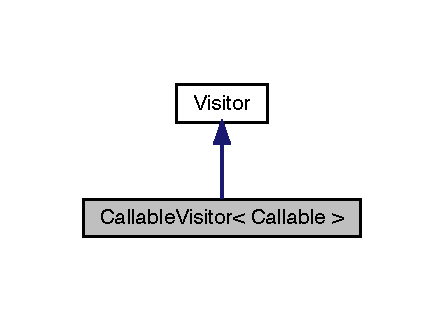
\includegraphics[width=213pt]{struct_callable_visitor__coll__graph}
\end{center}
\end{figure}
\subsection*{Public Member Functions}
\begin{DoxyCompactItemize}
\item 
\hyperlink{struct_callable_visitor_af9bd3a4132494b0c91dc4f7b46e5dd0e}{Callable\+Visitor} (Callable \hyperlink{struct_callable_visitor_a52ce52c399eb34a2a16abec3361e48b8}{callback})
\item 
{\footnotesize template$<$typename T $>$ }\\void \hyperlink{struct_callable_visitor_a4ce6de39a481c39fd7eda7a317bef28a}{call} (const T \&node)
\item 
void \hyperlink{struct_callable_visitor_ac435fdf6fcab885cf21f27364883c8ad}{operator()} (const \hyperlink{struct_this}{This} \&node) override
\item 
void \hyperlink{struct_callable_visitor_a83e70f05edc12de1717db28d2cd11cd5}{operator()} (const \hyperlink{struct_identifier}{Identifier} \&node) override
\item 
void \hyperlink{struct_callable_visitor_a5bce06c30e25d3a5498bc699f6e61ecc}{operator()} (const \hyperlink{struct_null_literal}{Null\+Literal} \&node) override
\item 
void \hyperlink{struct_callable_visitor_a76ea62da5cc85a9e301f68bb61d225c7}{operator()} (const \hyperlink{struct_boolean_literal}{Boolean\+Literal} \&node) override
\item 
void \hyperlink{struct_callable_visitor_a88418c625d814fd301125a640392fead}{operator()} (const \hyperlink{struct_numeric_literal}{Numeric\+Literal} \&node) override
\item 
void \hyperlink{struct_callable_visitor_a9746653850696a2060b0c2eeff8eaa69}{operator()} (const \hyperlink{struct_string_literal}{String\+Literal} \&node) override
\item 
void \hyperlink{struct_callable_visitor_ab3c41e1fb7ac9d411e3dc7c03c936851}{operator()} (const \hyperlink{struct_regular_expression_literal}{Regular\+Expression\+Literal} \&node) override
\item 
void \hyperlink{struct_callable_visitor_a01597431529a973c356ea13809ebc001}{operator()} (const \hyperlink{struct_array_literal}{Array\+Literal} \&node) override
\item 
void \hyperlink{struct_callable_visitor_ab3e67c6bb7d8332203e686d6aac59039}{operator()} (const \hyperlink{struct_object_literal}{Object\+Literal} \&node) override
\item 
void \hyperlink{struct_callable_visitor_a59d72c70fe06b87dfe5fdd9d53469ef2}{operator()} (const \hyperlink{struct_member_expression}{Member\+Expression} \&node) override
\item 
void \hyperlink{struct_callable_visitor_a2f9386232d6c45a5a15faf2a711895cd}{operator()} (const \hyperlink{struct_new_expression}{New\+Expression} \&node) override
\item 
void \hyperlink{struct_callable_visitor_a1cddd42d479e93e1a7e9693726e18dd5}{operator()} (const \hyperlink{struct_call_expression}{Call\+Expression} \&node) override
\item 
void \hyperlink{struct_callable_visitor_abc81c2b2a4765ac791bf6cd73ca97b9a}{operator()} (const \hyperlink{struct_postfix_expression}{Postfix\+Expression} \&node) override
\item 
void \hyperlink{struct_callable_visitor_a97c38a0a06a6f9ab527546060b518639}{operator()} (const \hyperlink{struct_unary_expression}{Unary\+Expression} \&node) override
\item 
void \hyperlink{struct_callable_visitor_ae926f418a357edc9dfebb0173b921029}{operator()} (const \hyperlink{struct_binary_expression}{Binary\+Expression} \&node) override
\item 
void \hyperlink{struct_callable_visitor_a239782df486cd64db0434955f114cb43}{operator()} (const \hyperlink{struct_conditional_expression}{Conditional\+Expression} \&node) override
\item 
void \hyperlink{struct_callable_visitor_ae27a0a08ee7eaa1956bd9e43da01ee4f}{operator()} (const \hyperlink{struct_function_expression}{Function\+Expression} \&node) override
\item 
void \hyperlink{struct_callable_visitor_a4ad3a74aae8cb9f1b4a8deb6d5738ccc}{operator()} (const \hyperlink{struct_block}{Block} \&node) override
\item 
void \hyperlink{struct_callable_visitor_a953a21e9aab73b9104355c2d04b3f79d}{operator()} (const \hyperlink{struct_variable_statement}{Variable\+Statement} \&node) override
\item 
void \hyperlink{struct_callable_visitor_a71422a8c5db1c1f6e73dd76638a2a47b}{operator()} (const \hyperlink{struct_empty_statement}{Empty\+Statement} \&node) override
\item 
void \hyperlink{struct_callable_visitor_ae09660080883ac12939e8b9581113e9c}{operator()} (const \hyperlink{struct_expression_statement}{Expression\+Statement} \&node) override
\item 
void \hyperlink{struct_callable_visitor_a5aaa91de3ead2c42bed03df3fa0de990}{operator()} (const \hyperlink{struct_if_statement}{If\+Statement} \&node) override
\item 
void \hyperlink{struct_callable_visitor_a02bd47f3f8baf9ba24530d4622dc137d}{operator()} (const \hyperlink{struct_do_while_statement}{Do\+While\+Statement} \&node) override
\item 
void \hyperlink{struct_callable_visitor_adffa6fa6621caae9474604fafb91fdfd}{operator()} (const \hyperlink{struct_while_statement}{While\+Statement} \&node) override
\item 
void \hyperlink{struct_callable_visitor_a78b5cf2f0db8eb174097f4fcc8618b75}{operator()} (const \hyperlink{struct_for_statement}{For\+Statement} \&node) override
\item 
void \hyperlink{struct_callable_visitor_a45b8579f057d5566ad016f667cf2c068}{operator()} (const \hyperlink{struct_for_in_statement}{For\+In\+Statement} \&node) override
\item 
void \hyperlink{struct_callable_visitor_a15e41131b34e8d1a54b3af9719287248}{operator()} (const \hyperlink{struct_continue_statement}{Continue\+Statement} \&node) override
\item 
void \hyperlink{struct_callable_visitor_a3281651a229ad1e156aba9216bb64cec}{operator()} (const \hyperlink{struct_break_statement}{Break\+Statement} \&node) override
\item 
void \hyperlink{struct_callable_visitor_aebfd735e24e1161b3414d1bd5ad31cd5}{operator()} (const \hyperlink{struct_return_statement}{Return\+Statement} \&node) override
\item 
void \hyperlink{struct_callable_visitor_a08a6aec153b2e3b25b53642a6b9c7aab}{operator()} (const \hyperlink{struct_with_statement}{With\+Statement} \&node) override
\item 
void \hyperlink{struct_callable_visitor_a75929176e0ea51e67f01ed53d53bfa18}{operator()} (const \hyperlink{struct_labelled_statement}{Labelled\+Statement} \&node) override
\item 
void \hyperlink{struct_callable_visitor_a22380f6060601822b4c2f316d32c20a5}{operator()} (const \hyperlink{struct_switch_statement}{Switch\+Statement} \&node) override
\item 
void \hyperlink{struct_callable_visitor_af7d629f3f0fa66e3e8e38bd76c6cc729}{operator()} (const \hyperlink{struct_throw_statement}{Throw\+Statement} \&node) override
\item 
void \hyperlink{struct_callable_visitor_ae06c85aae9971525a8b880c5a398c8e3}{operator()} (const \hyperlink{struct_try_statement}{Try\+Statement} \&node) override
\item 
void \hyperlink{struct_callable_visitor_a5e2b63226fc91e23d9e59ec1ad4914c6}{operator()} (const \hyperlink{struct_debugger_statement}{Debugger\+Statement} \&node) override
\item 
void \hyperlink{struct_callable_visitor_a61efb29b38c0b4a1a46e392f1133013c}{operator()} (const \hyperlink{struct_case_clause}{Case\+Clause} \&node) override
\item 
void \hyperlink{struct_callable_visitor_ace58d18d6b2e0d27489b365db59e31ae}{operator()} (const \hyperlink{struct_default_clause}{Default\+Clause} \&node) override
\item 
void \hyperlink{struct_callable_visitor_a7d3ebcc10e02e0c9698170d957241846}{operator()} (const \hyperlink{struct_function_declaration}{Function\+Declaration} \&node) override
\item 
void \hyperlink{struct_callable_visitor_a81403b11d510563427191958e7a04d0b}{operator()} (const \hyperlink{struct_variable_declaration}{Variable\+Declaration} \&node) override
\item 
void \hyperlink{struct_callable_visitor_a72a62905dbd6c37719ab422462d7b8f5}{operator()} (const \hyperlink{struct_elision}{Elision} \&node) override
\item 
void \hyperlink{struct_callable_visitor_a2034a4d5531273c87f3fefbec8db6970}{operator()} (const \hyperlink{struct_property_name}{Property\+Name} \&node) override
\item 
void \hyperlink{struct_callable_visitor_aa88ba8cf86d84ccbc23c995ecf87bea8}{operator()} (const \hyperlink{struct_property_assignment}{Property\+Assignment} \&node) override
\item 
void \hyperlink{struct_callable_visitor_aa70a97d5a44ecc30aac8fb97c12cabb6}{operator()} (const \hyperlink{struct_arguments}{Arguments} \&node) override
\item 
void \hyperlink{struct_callable_visitor_a37e48e9df8cb4cff6bc135e7402a7244}{operator()} (const \hyperlink{struct_program}{Program} \&node) override
\end{DoxyCompactItemize}
\subsection*{Public Attributes}
\begin{DoxyCompactItemize}
\item 
Callable \hyperlink{struct_callable_visitor_a52ce52c399eb34a2a16abec3361e48b8}{callback}
\end{DoxyCompactItemize}


\subsection{Constructor \& Destructor Documentation}
\mbox{\Hypertarget{struct_callable_visitor_af9bd3a4132494b0c91dc4f7b46e5dd0e}\label{struct_callable_visitor_af9bd3a4132494b0c91dc4f7b46e5dd0e}} 
\index{Callable\+Visitor@{Callable\+Visitor}!Callable\+Visitor@{Callable\+Visitor}}
\index{Callable\+Visitor@{Callable\+Visitor}!Callable\+Visitor@{Callable\+Visitor}}
\subsubsection{\texorpdfstring{Callable\+Visitor()}{CallableVisitor()}}
{\footnotesize\ttfamily template$<$typename Callable $>$ \\
\hyperlink{struct_callable_visitor}{Callable\+Visitor}$<$ Callable $>$\+::\hyperlink{struct_callable_visitor}{Callable\+Visitor} (\begin{DoxyParamCaption}\item[{Callable}]{callback }\end{DoxyParamCaption})\hspace{0.3cm}{\ttfamily [inline]}}



\subsection{Member Function Documentation}
\mbox{\Hypertarget{struct_callable_visitor_a4ce6de39a481c39fd7eda7a317bef28a}\label{struct_callable_visitor_a4ce6de39a481c39fd7eda7a317bef28a}} 
\index{Callable\+Visitor@{Callable\+Visitor}!call@{call}}
\index{call@{call}!Callable\+Visitor@{Callable\+Visitor}}
\subsubsection{\texorpdfstring{call()}{call()}}
{\footnotesize\ttfamily template$<$typename Callable $>$ \\
template$<$typename T $>$ \\
void \hyperlink{struct_callable_visitor}{Callable\+Visitor}$<$ Callable $>$\+::call (\begin{DoxyParamCaption}\item[{const T \&}]{node }\end{DoxyParamCaption})\hspace{0.3cm}{\ttfamily [inline]}}

\mbox{\Hypertarget{struct_callable_visitor_ac435fdf6fcab885cf21f27364883c8ad}\label{struct_callable_visitor_ac435fdf6fcab885cf21f27364883c8ad}} 
\index{Callable\+Visitor@{Callable\+Visitor}!operator()@{operator()}}
\index{operator()@{operator()}!Callable\+Visitor@{Callable\+Visitor}}
\subsubsection{\texorpdfstring{operator()()}{operator()()}\hspace{0.1cm}{\footnotesize\ttfamily [1/44]}}
{\footnotesize\ttfamily template$<$typename Callable $>$ \\
void \hyperlink{struct_callable_visitor}{Callable\+Visitor}$<$ Callable $>$\+::operator() (\begin{DoxyParamCaption}\item[{const \hyperlink{struct_this}{This} \&}]{node }\end{DoxyParamCaption})\hspace{0.3cm}{\ttfamily [inline]}, {\ttfamily [override]}, {\ttfamily [virtual]}}



Implements \hyperlink{struct_visitor_a7a043c9da4e7f8233db48afb82dbc7bc}{Visitor}.

\mbox{\Hypertarget{struct_callable_visitor_a83e70f05edc12de1717db28d2cd11cd5}\label{struct_callable_visitor_a83e70f05edc12de1717db28d2cd11cd5}} 
\index{Callable\+Visitor@{Callable\+Visitor}!operator()@{operator()}}
\index{operator()@{operator()}!Callable\+Visitor@{Callable\+Visitor}}
\subsubsection{\texorpdfstring{operator()()}{operator()()}\hspace{0.1cm}{\footnotesize\ttfamily [2/44]}}
{\footnotesize\ttfamily template$<$typename Callable $>$ \\
void \hyperlink{struct_callable_visitor}{Callable\+Visitor}$<$ Callable $>$\+::operator() (\begin{DoxyParamCaption}\item[{const \hyperlink{struct_identifier}{Identifier} \&}]{node }\end{DoxyParamCaption})\hspace{0.3cm}{\ttfamily [inline]}, {\ttfamily [override]}, {\ttfamily [virtual]}}



Implements \hyperlink{struct_visitor_a2d09687aa24b1b618c6205f8413c2dd3}{Visitor}.

\mbox{\Hypertarget{struct_callable_visitor_a5bce06c30e25d3a5498bc699f6e61ecc}\label{struct_callable_visitor_a5bce06c30e25d3a5498bc699f6e61ecc}} 
\index{Callable\+Visitor@{Callable\+Visitor}!operator()@{operator()}}
\index{operator()@{operator()}!Callable\+Visitor@{Callable\+Visitor}}
\subsubsection{\texorpdfstring{operator()()}{operator()()}\hspace{0.1cm}{\footnotesize\ttfamily [3/44]}}
{\footnotesize\ttfamily template$<$typename Callable $>$ \\
void \hyperlink{struct_callable_visitor}{Callable\+Visitor}$<$ Callable $>$\+::operator() (\begin{DoxyParamCaption}\item[{const \hyperlink{struct_null_literal}{Null\+Literal} \&}]{node }\end{DoxyParamCaption})\hspace{0.3cm}{\ttfamily [inline]}, {\ttfamily [override]}, {\ttfamily [virtual]}}



Implements \hyperlink{struct_visitor_a2278ee24407bdc0d3addf887754d4c6c}{Visitor}.

\mbox{\Hypertarget{struct_callable_visitor_a76ea62da5cc85a9e301f68bb61d225c7}\label{struct_callable_visitor_a76ea62da5cc85a9e301f68bb61d225c7}} 
\index{Callable\+Visitor@{Callable\+Visitor}!operator()@{operator()}}
\index{operator()@{operator()}!Callable\+Visitor@{Callable\+Visitor}}
\subsubsection{\texorpdfstring{operator()()}{operator()()}\hspace{0.1cm}{\footnotesize\ttfamily [4/44]}}
{\footnotesize\ttfamily template$<$typename Callable $>$ \\
void \hyperlink{struct_callable_visitor}{Callable\+Visitor}$<$ Callable $>$\+::operator() (\begin{DoxyParamCaption}\item[{const \hyperlink{struct_boolean_literal}{Boolean\+Literal} \&}]{node }\end{DoxyParamCaption})\hspace{0.3cm}{\ttfamily [inline]}, {\ttfamily [override]}, {\ttfamily [virtual]}}



Implements \hyperlink{struct_visitor_af3b394eaf1b9b1db22379aedcb234a2f}{Visitor}.

\mbox{\Hypertarget{struct_callable_visitor_a88418c625d814fd301125a640392fead}\label{struct_callable_visitor_a88418c625d814fd301125a640392fead}} 
\index{Callable\+Visitor@{Callable\+Visitor}!operator()@{operator()}}
\index{operator()@{operator()}!Callable\+Visitor@{Callable\+Visitor}}
\subsubsection{\texorpdfstring{operator()()}{operator()()}\hspace{0.1cm}{\footnotesize\ttfamily [5/44]}}
{\footnotesize\ttfamily template$<$typename Callable $>$ \\
void \hyperlink{struct_callable_visitor}{Callable\+Visitor}$<$ Callable $>$\+::operator() (\begin{DoxyParamCaption}\item[{const \hyperlink{struct_numeric_literal}{Numeric\+Literal} \&}]{node }\end{DoxyParamCaption})\hspace{0.3cm}{\ttfamily [inline]}, {\ttfamily [override]}, {\ttfamily [virtual]}}



Implements \hyperlink{struct_visitor_a6d707fe0c1563b39aae3ecd7ddb5ab8f}{Visitor}.

\mbox{\Hypertarget{struct_callable_visitor_a9746653850696a2060b0c2eeff8eaa69}\label{struct_callable_visitor_a9746653850696a2060b0c2eeff8eaa69}} 
\index{Callable\+Visitor@{Callable\+Visitor}!operator()@{operator()}}
\index{operator()@{operator()}!Callable\+Visitor@{Callable\+Visitor}}
\subsubsection{\texorpdfstring{operator()()}{operator()()}\hspace{0.1cm}{\footnotesize\ttfamily [6/44]}}
{\footnotesize\ttfamily template$<$typename Callable $>$ \\
void \hyperlink{struct_callable_visitor}{Callable\+Visitor}$<$ Callable $>$\+::operator() (\begin{DoxyParamCaption}\item[{const \hyperlink{struct_string_literal}{String\+Literal} \&}]{node }\end{DoxyParamCaption})\hspace{0.3cm}{\ttfamily [inline]}, {\ttfamily [override]}, {\ttfamily [virtual]}}



Implements \hyperlink{struct_visitor_a6bab8ba66edf0cc73cb92073269e7848}{Visitor}.

\mbox{\Hypertarget{struct_callable_visitor_ab3c41e1fb7ac9d411e3dc7c03c936851}\label{struct_callable_visitor_ab3c41e1fb7ac9d411e3dc7c03c936851}} 
\index{Callable\+Visitor@{Callable\+Visitor}!operator()@{operator()}}
\index{operator()@{operator()}!Callable\+Visitor@{Callable\+Visitor}}
\subsubsection{\texorpdfstring{operator()()}{operator()()}\hspace{0.1cm}{\footnotesize\ttfamily [7/44]}}
{\footnotesize\ttfamily template$<$typename Callable $>$ \\
void \hyperlink{struct_callable_visitor}{Callable\+Visitor}$<$ Callable $>$\+::operator() (\begin{DoxyParamCaption}\item[{const \hyperlink{struct_regular_expression_literal}{Regular\+Expression\+Literal} \&}]{node }\end{DoxyParamCaption})\hspace{0.3cm}{\ttfamily [inline]}, {\ttfamily [override]}, {\ttfamily [virtual]}}



Implements \hyperlink{struct_visitor_aea90f9399628f301f8c25a62ce268097}{Visitor}.

\mbox{\Hypertarget{struct_callable_visitor_a01597431529a973c356ea13809ebc001}\label{struct_callable_visitor_a01597431529a973c356ea13809ebc001}} 
\index{Callable\+Visitor@{Callable\+Visitor}!operator()@{operator()}}
\index{operator()@{operator()}!Callable\+Visitor@{Callable\+Visitor}}
\subsubsection{\texorpdfstring{operator()()}{operator()()}\hspace{0.1cm}{\footnotesize\ttfamily [8/44]}}
{\footnotesize\ttfamily template$<$typename Callable $>$ \\
void \hyperlink{struct_callable_visitor}{Callable\+Visitor}$<$ Callable $>$\+::operator() (\begin{DoxyParamCaption}\item[{const \hyperlink{struct_array_literal}{Array\+Literal} \&}]{node }\end{DoxyParamCaption})\hspace{0.3cm}{\ttfamily [inline]}, {\ttfamily [override]}, {\ttfamily [virtual]}}



Implements \hyperlink{struct_visitor_a46f9846468f2c12ddc585cfe0421e6f0}{Visitor}.

\mbox{\Hypertarget{struct_callable_visitor_ab3e67c6bb7d8332203e686d6aac59039}\label{struct_callable_visitor_ab3e67c6bb7d8332203e686d6aac59039}} 
\index{Callable\+Visitor@{Callable\+Visitor}!operator()@{operator()}}
\index{operator()@{operator()}!Callable\+Visitor@{Callable\+Visitor}}
\subsubsection{\texorpdfstring{operator()()}{operator()()}\hspace{0.1cm}{\footnotesize\ttfamily [9/44]}}
{\footnotesize\ttfamily template$<$typename Callable $>$ \\
void \hyperlink{struct_callable_visitor}{Callable\+Visitor}$<$ Callable $>$\+::operator() (\begin{DoxyParamCaption}\item[{const \hyperlink{struct_object_literal}{Object\+Literal} \&}]{node }\end{DoxyParamCaption})\hspace{0.3cm}{\ttfamily [inline]}, {\ttfamily [override]}, {\ttfamily [virtual]}}



Implements \hyperlink{struct_visitor_ad85d9aa9718801a1a8233cf51d8f7055}{Visitor}.

\mbox{\Hypertarget{struct_callable_visitor_a59d72c70fe06b87dfe5fdd9d53469ef2}\label{struct_callable_visitor_a59d72c70fe06b87dfe5fdd9d53469ef2}} 
\index{Callable\+Visitor@{Callable\+Visitor}!operator()@{operator()}}
\index{operator()@{operator()}!Callable\+Visitor@{Callable\+Visitor}}
\subsubsection{\texorpdfstring{operator()()}{operator()()}\hspace{0.1cm}{\footnotesize\ttfamily [10/44]}}
{\footnotesize\ttfamily template$<$typename Callable $>$ \\
void \hyperlink{struct_callable_visitor}{Callable\+Visitor}$<$ Callable $>$\+::operator() (\begin{DoxyParamCaption}\item[{const \hyperlink{struct_member_expression}{Member\+Expression} \&}]{node }\end{DoxyParamCaption})\hspace{0.3cm}{\ttfamily [inline]}, {\ttfamily [override]}, {\ttfamily [virtual]}}



Implements \hyperlink{struct_visitor_a175fd29619240cc378703de4c357f348}{Visitor}.

\mbox{\Hypertarget{struct_callable_visitor_a2f9386232d6c45a5a15faf2a711895cd}\label{struct_callable_visitor_a2f9386232d6c45a5a15faf2a711895cd}} 
\index{Callable\+Visitor@{Callable\+Visitor}!operator()@{operator()}}
\index{operator()@{operator()}!Callable\+Visitor@{Callable\+Visitor}}
\subsubsection{\texorpdfstring{operator()()}{operator()()}\hspace{0.1cm}{\footnotesize\ttfamily [11/44]}}
{\footnotesize\ttfamily template$<$typename Callable $>$ \\
void \hyperlink{struct_callable_visitor}{Callable\+Visitor}$<$ Callable $>$\+::operator() (\begin{DoxyParamCaption}\item[{const \hyperlink{struct_new_expression}{New\+Expression} \&}]{node }\end{DoxyParamCaption})\hspace{0.3cm}{\ttfamily [inline]}, {\ttfamily [override]}, {\ttfamily [virtual]}}



Implements \hyperlink{struct_visitor_a13ead8d5ef82f284e301ba8127e9fb56}{Visitor}.

\mbox{\Hypertarget{struct_callable_visitor_a1cddd42d479e93e1a7e9693726e18dd5}\label{struct_callable_visitor_a1cddd42d479e93e1a7e9693726e18dd5}} 
\index{Callable\+Visitor@{Callable\+Visitor}!operator()@{operator()}}
\index{operator()@{operator()}!Callable\+Visitor@{Callable\+Visitor}}
\subsubsection{\texorpdfstring{operator()()}{operator()()}\hspace{0.1cm}{\footnotesize\ttfamily [12/44]}}
{\footnotesize\ttfamily template$<$typename Callable $>$ \\
void \hyperlink{struct_callable_visitor}{Callable\+Visitor}$<$ Callable $>$\+::operator() (\begin{DoxyParamCaption}\item[{const \hyperlink{struct_call_expression}{Call\+Expression} \&}]{node }\end{DoxyParamCaption})\hspace{0.3cm}{\ttfamily [inline]}, {\ttfamily [override]}, {\ttfamily [virtual]}}



Implements \hyperlink{struct_visitor_aa6152c6f355690fd1c4db37fff303614}{Visitor}.

\mbox{\Hypertarget{struct_callable_visitor_abc81c2b2a4765ac791bf6cd73ca97b9a}\label{struct_callable_visitor_abc81c2b2a4765ac791bf6cd73ca97b9a}} 
\index{Callable\+Visitor@{Callable\+Visitor}!operator()@{operator()}}
\index{operator()@{operator()}!Callable\+Visitor@{Callable\+Visitor}}
\subsubsection{\texorpdfstring{operator()()}{operator()()}\hspace{0.1cm}{\footnotesize\ttfamily [13/44]}}
{\footnotesize\ttfamily template$<$typename Callable $>$ \\
void \hyperlink{struct_callable_visitor}{Callable\+Visitor}$<$ Callable $>$\+::operator() (\begin{DoxyParamCaption}\item[{const \hyperlink{struct_postfix_expression}{Postfix\+Expression} \&}]{node }\end{DoxyParamCaption})\hspace{0.3cm}{\ttfamily [inline]}, {\ttfamily [override]}, {\ttfamily [virtual]}}



Implements \hyperlink{struct_visitor_acd630c29940c6785726ce51c7db0aab9}{Visitor}.

\mbox{\Hypertarget{struct_callable_visitor_a97c38a0a06a6f9ab527546060b518639}\label{struct_callable_visitor_a97c38a0a06a6f9ab527546060b518639}} 
\index{Callable\+Visitor@{Callable\+Visitor}!operator()@{operator()}}
\index{operator()@{operator()}!Callable\+Visitor@{Callable\+Visitor}}
\subsubsection{\texorpdfstring{operator()()}{operator()()}\hspace{0.1cm}{\footnotesize\ttfamily [14/44]}}
{\footnotesize\ttfamily template$<$typename Callable $>$ \\
void \hyperlink{struct_callable_visitor}{Callable\+Visitor}$<$ Callable $>$\+::operator() (\begin{DoxyParamCaption}\item[{const \hyperlink{struct_unary_expression}{Unary\+Expression} \&}]{node }\end{DoxyParamCaption})\hspace{0.3cm}{\ttfamily [inline]}, {\ttfamily [override]}, {\ttfamily [virtual]}}



Implements \hyperlink{struct_visitor_ad2e06814dadca4469f4036ba9a00afd7}{Visitor}.

\mbox{\Hypertarget{struct_callable_visitor_ae926f418a357edc9dfebb0173b921029}\label{struct_callable_visitor_ae926f418a357edc9dfebb0173b921029}} 
\index{Callable\+Visitor@{Callable\+Visitor}!operator()@{operator()}}
\index{operator()@{operator()}!Callable\+Visitor@{Callable\+Visitor}}
\subsubsection{\texorpdfstring{operator()()}{operator()()}\hspace{0.1cm}{\footnotesize\ttfamily [15/44]}}
{\footnotesize\ttfamily template$<$typename Callable $>$ \\
void \hyperlink{struct_callable_visitor}{Callable\+Visitor}$<$ Callable $>$\+::operator() (\begin{DoxyParamCaption}\item[{const \hyperlink{struct_binary_expression}{Binary\+Expression} \&}]{node }\end{DoxyParamCaption})\hspace{0.3cm}{\ttfamily [inline]}, {\ttfamily [override]}, {\ttfamily [virtual]}}



Implements \hyperlink{struct_visitor_a6132b5969ec220e7c98af3a957f48a0e}{Visitor}.

\mbox{\Hypertarget{struct_callable_visitor_a239782df486cd64db0434955f114cb43}\label{struct_callable_visitor_a239782df486cd64db0434955f114cb43}} 
\index{Callable\+Visitor@{Callable\+Visitor}!operator()@{operator()}}
\index{operator()@{operator()}!Callable\+Visitor@{Callable\+Visitor}}
\subsubsection{\texorpdfstring{operator()()}{operator()()}\hspace{0.1cm}{\footnotesize\ttfamily [16/44]}}
{\footnotesize\ttfamily template$<$typename Callable $>$ \\
void \hyperlink{struct_callable_visitor}{Callable\+Visitor}$<$ Callable $>$\+::operator() (\begin{DoxyParamCaption}\item[{const \hyperlink{struct_conditional_expression}{Conditional\+Expression} \&}]{node }\end{DoxyParamCaption})\hspace{0.3cm}{\ttfamily [inline]}, {\ttfamily [override]}, {\ttfamily [virtual]}}



Implements \hyperlink{struct_visitor_a132fc5e3ff45efb2869272fbe5d5f815}{Visitor}.

\mbox{\Hypertarget{struct_callable_visitor_ae27a0a08ee7eaa1956bd9e43da01ee4f}\label{struct_callable_visitor_ae27a0a08ee7eaa1956bd9e43da01ee4f}} 
\index{Callable\+Visitor@{Callable\+Visitor}!operator()@{operator()}}
\index{operator()@{operator()}!Callable\+Visitor@{Callable\+Visitor}}
\subsubsection{\texorpdfstring{operator()()}{operator()()}\hspace{0.1cm}{\footnotesize\ttfamily [17/44]}}
{\footnotesize\ttfamily template$<$typename Callable $>$ \\
void \hyperlink{struct_callable_visitor}{Callable\+Visitor}$<$ Callable $>$\+::operator() (\begin{DoxyParamCaption}\item[{const \hyperlink{struct_function_expression}{Function\+Expression} \&}]{node }\end{DoxyParamCaption})\hspace{0.3cm}{\ttfamily [inline]}, {\ttfamily [override]}, {\ttfamily [virtual]}}



Implements \hyperlink{struct_visitor_a3f6eb67942d7e2c83a761de2bd66a60a}{Visitor}.

\mbox{\Hypertarget{struct_callable_visitor_a4ad3a74aae8cb9f1b4a8deb6d5738ccc}\label{struct_callable_visitor_a4ad3a74aae8cb9f1b4a8deb6d5738ccc}} 
\index{Callable\+Visitor@{Callable\+Visitor}!operator()@{operator()}}
\index{operator()@{operator()}!Callable\+Visitor@{Callable\+Visitor}}
\subsubsection{\texorpdfstring{operator()()}{operator()()}\hspace{0.1cm}{\footnotesize\ttfamily [18/44]}}
{\footnotesize\ttfamily template$<$typename Callable $>$ \\
void \hyperlink{struct_callable_visitor}{Callable\+Visitor}$<$ Callable $>$\+::operator() (\begin{DoxyParamCaption}\item[{const \hyperlink{struct_block}{Block} \&}]{node }\end{DoxyParamCaption})\hspace{0.3cm}{\ttfamily [inline]}, {\ttfamily [override]}, {\ttfamily [virtual]}}



Implements \hyperlink{struct_visitor_a3a26b45c1ab418661f992d97ed9ec9f0}{Visitor}.

\mbox{\Hypertarget{struct_callable_visitor_a953a21e9aab73b9104355c2d04b3f79d}\label{struct_callable_visitor_a953a21e9aab73b9104355c2d04b3f79d}} 
\index{Callable\+Visitor@{Callable\+Visitor}!operator()@{operator()}}
\index{operator()@{operator()}!Callable\+Visitor@{Callable\+Visitor}}
\subsubsection{\texorpdfstring{operator()()}{operator()()}\hspace{0.1cm}{\footnotesize\ttfamily [19/44]}}
{\footnotesize\ttfamily template$<$typename Callable $>$ \\
void \hyperlink{struct_callable_visitor}{Callable\+Visitor}$<$ Callable $>$\+::operator() (\begin{DoxyParamCaption}\item[{const \hyperlink{struct_variable_statement}{Variable\+Statement} \&}]{node }\end{DoxyParamCaption})\hspace{0.3cm}{\ttfamily [inline]}, {\ttfamily [override]}, {\ttfamily [virtual]}}



Implements \hyperlink{struct_visitor_accbed2e228126d93b162df7bb44bb3c8}{Visitor}.

\mbox{\Hypertarget{struct_callable_visitor_a71422a8c5db1c1f6e73dd76638a2a47b}\label{struct_callable_visitor_a71422a8c5db1c1f6e73dd76638a2a47b}} 
\index{Callable\+Visitor@{Callable\+Visitor}!operator()@{operator()}}
\index{operator()@{operator()}!Callable\+Visitor@{Callable\+Visitor}}
\subsubsection{\texorpdfstring{operator()()}{operator()()}\hspace{0.1cm}{\footnotesize\ttfamily [20/44]}}
{\footnotesize\ttfamily template$<$typename Callable $>$ \\
void \hyperlink{struct_callable_visitor}{Callable\+Visitor}$<$ Callable $>$\+::operator() (\begin{DoxyParamCaption}\item[{const \hyperlink{struct_empty_statement}{Empty\+Statement} \&}]{node }\end{DoxyParamCaption})\hspace{0.3cm}{\ttfamily [inline]}, {\ttfamily [override]}, {\ttfamily [virtual]}}



Implements \hyperlink{struct_visitor_a67719a8d9005a86141e4cb9226c11ca4}{Visitor}.

\mbox{\Hypertarget{struct_callable_visitor_ae09660080883ac12939e8b9581113e9c}\label{struct_callable_visitor_ae09660080883ac12939e8b9581113e9c}} 
\index{Callable\+Visitor@{Callable\+Visitor}!operator()@{operator()}}
\index{operator()@{operator()}!Callable\+Visitor@{Callable\+Visitor}}
\subsubsection{\texorpdfstring{operator()()}{operator()()}\hspace{0.1cm}{\footnotesize\ttfamily [21/44]}}
{\footnotesize\ttfamily template$<$typename Callable $>$ \\
void \hyperlink{struct_callable_visitor}{Callable\+Visitor}$<$ Callable $>$\+::operator() (\begin{DoxyParamCaption}\item[{const \hyperlink{struct_expression_statement}{Expression\+Statement} \&}]{node }\end{DoxyParamCaption})\hspace{0.3cm}{\ttfamily [inline]}, {\ttfamily [override]}, {\ttfamily [virtual]}}



Implements \hyperlink{struct_visitor_a319554fbb3f24e664a86ef7839201040}{Visitor}.

\mbox{\Hypertarget{struct_callable_visitor_a5aaa91de3ead2c42bed03df3fa0de990}\label{struct_callable_visitor_a5aaa91de3ead2c42bed03df3fa0de990}} 
\index{Callable\+Visitor@{Callable\+Visitor}!operator()@{operator()}}
\index{operator()@{operator()}!Callable\+Visitor@{Callable\+Visitor}}
\subsubsection{\texorpdfstring{operator()()}{operator()()}\hspace{0.1cm}{\footnotesize\ttfamily [22/44]}}
{\footnotesize\ttfamily template$<$typename Callable $>$ \\
void \hyperlink{struct_callable_visitor}{Callable\+Visitor}$<$ Callable $>$\+::operator() (\begin{DoxyParamCaption}\item[{const \hyperlink{struct_if_statement}{If\+Statement} \&}]{node }\end{DoxyParamCaption})\hspace{0.3cm}{\ttfamily [inline]}, {\ttfamily [override]}, {\ttfamily [virtual]}}



Implements \hyperlink{struct_visitor_a9d30bc5ad73a274f7533df4b5a65ae41}{Visitor}.

\mbox{\Hypertarget{struct_callable_visitor_a02bd47f3f8baf9ba24530d4622dc137d}\label{struct_callable_visitor_a02bd47f3f8baf9ba24530d4622dc137d}} 
\index{Callable\+Visitor@{Callable\+Visitor}!operator()@{operator()}}
\index{operator()@{operator()}!Callable\+Visitor@{Callable\+Visitor}}
\subsubsection{\texorpdfstring{operator()()}{operator()()}\hspace{0.1cm}{\footnotesize\ttfamily [23/44]}}
{\footnotesize\ttfamily template$<$typename Callable $>$ \\
void \hyperlink{struct_callable_visitor}{Callable\+Visitor}$<$ Callable $>$\+::operator() (\begin{DoxyParamCaption}\item[{const \hyperlink{struct_do_while_statement}{Do\+While\+Statement} \&}]{node }\end{DoxyParamCaption})\hspace{0.3cm}{\ttfamily [inline]}, {\ttfamily [override]}, {\ttfamily [virtual]}}



Implements \hyperlink{struct_visitor_a077a0025430c4b35d310bdfcbe1b180a}{Visitor}.

\mbox{\Hypertarget{struct_callable_visitor_adffa6fa6621caae9474604fafb91fdfd}\label{struct_callable_visitor_adffa6fa6621caae9474604fafb91fdfd}} 
\index{Callable\+Visitor@{Callable\+Visitor}!operator()@{operator()}}
\index{operator()@{operator()}!Callable\+Visitor@{Callable\+Visitor}}
\subsubsection{\texorpdfstring{operator()()}{operator()()}\hspace{0.1cm}{\footnotesize\ttfamily [24/44]}}
{\footnotesize\ttfamily template$<$typename Callable $>$ \\
void \hyperlink{struct_callable_visitor}{Callable\+Visitor}$<$ Callable $>$\+::operator() (\begin{DoxyParamCaption}\item[{const \hyperlink{struct_while_statement}{While\+Statement} \&}]{node }\end{DoxyParamCaption})\hspace{0.3cm}{\ttfamily [inline]}, {\ttfamily [override]}, {\ttfamily [virtual]}}



Implements \hyperlink{struct_visitor_a4faef50c61a3c1246589390d925c2f53}{Visitor}.

\mbox{\Hypertarget{struct_callable_visitor_a78b5cf2f0db8eb174097f4fcc8618b75}\label{struct_callable_visitor_a78b5cf2f0db8eb174097f4fcc8618b75}} 
\index{Callable\+Visitor@{Callable\+Visitor}!operator()@{operator()}}
\index{operator()@{operator()}!Callable\+Visitor@{Callable\+Visitor}}
\subsubsection{\texorpdfstring{operator()()}{operator()()}\hspace{0.1cm}{\footnotesize\ttfamily [25/44]}}
{\footnotesize\ttfamily template$<$typename Callable $>$ \\
void \hyperlink{struct_callable_visitor}{Callable\+Visitor}$<$ Callable $>$\+::operator() (\begin{DoxyParamCaption}\item[{const \hyperlink{struct_for_statement}{For\+Statement} \&}]{node }\end{DoxyParamCaption})\hspace{0.3cm}{\ttfamily [inline]}, {\ttfamily [override]}, {\ttfamily [virtual]}}



Implements \hyperlink{struct_visitor_a75180858faf5152f99742e4a19757928}{Visitor}.

\mbox{\Hypertarget{struct_callable_visitor_a45b8579f057d5566ad016f667cf2c068}\label{struct_callable_visitor_a45b8579f057d5566ad016f667cf2c068}} 
\index{Callable\+Visitor@{Callable\+Visitor}!operator()@{operator()}}
\index{operator()@{operator()}!Callable\+Visitor@{Callable\+Visitor}}
\subsubsection{\texorpdfstring{operator()()}{operator()()}\hspace{0.1cm}{\footnotesize\ttfamily [26/44]}}
{\footnotesize\ttfamily template$<$typename Callable $>$ \\
void \hyperlink{struct_callable_visitor}{Callable\+Visitor}$<$ Callable $>$\+::operator() (\begin{DoxyParamCaption}\item[{const \hyperlink{struct_for_in_statement}{For\+In\+Statement} \&}]{node }\end{DoxyParamCaption})\hspace{0.3cm}{\ttfamily [inline]}, {\ttfamily [override]}, {\ttfamily [virtual]}}



Implements \hyperlink{struct_visitor_af1c6c55ccfae8b2741e12168d81c45cb}{Visitor}.

\mbox{\Hypertarget{struct_callable_visitor_a15e41131b34e8d1a54b3af9719287248}\label{struct_callable_visitor_a15e41131b34e8d1a54b3af9719287248}} 
\index{Callable\+Visitor@{Callable\+Visitor}!operator()@{operator()}}
\index{operator()@{operator()}!Callable\+Visitor@{Callable\+Visitor}}
\subsubsection{\texorpdfstring{operator()()}{operator()()}\hspace{0.1cm}{\footnotesize\ttfamily [27/44]}}
{\footnotesize\ttfamily template$<$typename Callable $>$ \\
void \hyperlink{struct_callable_visitor}{Callable\+Visitor}$<$ Callable $>$\+::operator() (\begin{DoxyParamCaption}\item[{const \hyperlink{struct_continue_statement}{Continue\+Statement} \&}]{node }\end{DoxyParamCaption})\hspace{0.3cm}{\ttfamily [inline]}, {\ttfamily [override]}, {\ttfamily [virtual]}}



Implements \hyperlink{struct_visitor_aca30136319d28baf708663a1d823af3a}{Visitor}.

\mbox{\Hypertarget{struct_callable_visitor_a3281651a229ad1e156aba9216bb64cec}\label{struct_callable_visitor_a3281651a229ad1e156aba9216bb64cec}} 
\index{Callable\+Visitor@{Callable\+Visitor}!operator()@{operator()}}
\index{operator()@{operator()}!Callable\+Visitor@{Callable\+Visitor}}
\subsubsection{\texorpdfstring{operator()()}{operator()()}\hspace{0.1cm}{\footnotesize\ttfamily [28/44]}}
{\footnotesize\ttfamily template$<$typename Callable $>$ \\
void \hyperlink{struct_callable_visitor}{Callable\+Visitor}$<$ Callable $>$\+::operator() (\begin{DoxyParamCaption}\item[{const \hyperlink{struct_break_statement}{Break\+Statement} \&}]{node }\end{DoxyParamCaption})\hspace{0.3cm}{\ttfamily [inline]}, {\ttfamily [override]}, {\ttfamily [virtual]}}



Implements \hyperlink{struct_visitor_a19997436906171d41bec562d9cf260ef}{Visitor}.

\mbox{\Hypertarget{struct_callable_visitor_aebfd735e24e1161b3414d1bd5ad31cd5}\label{struct_callable_visitor_aebfd735e24e1161b3414d1bd5ad31cd5}} 
\index{Callable\+Visitor@{Callable\+Visitor}!operator()@{operator()}}
\index{operator()@{operator()}!Callable\+Visitor@{Callable\+Visitor}}
\subsubsection{\texorpdfstring{operator()()}{operator()()}\hspace{0.1cm}{\footnotesize\ttfamily [29/44]}}
{\footnotesize\ttfamily template$<$typename Callable $>$ \\
void \hyperlink{struct_callable_visitor}{Callable\+Visitor}$<$ Callable $>$\+::operator() (\begin{DoxyParamCaption}\item[{const \hyperlink{struct_return_statement}{Return\+Statement} \&}]{node }\end{DoxyParamCaption})\hspace{0.3cm}{\ttfamily [inline]}, {\ttfamily [override]}, {\ttfamily [virtual]}}



Implements \hyperlink{struct_visitor_a041431785a00f9f387c7bc670b3ac660}{Visitor}.

\mbox{\Hypertarget{struct_callable_visitor_a08a6aec153b2e3b25b53642a6b9c7aab}\label{struct_callable_visitor_a08a6aec153b2e3b25b53642a6b9c7aab}} 
\index{Callable\+Visitor@{Callable\+Visitor}!operator()@{operator()}}
\index{operator()@{operator()}!Callable\+Visitor@{Callable\+Visitor}}
\subsubsection{\texorpdfstring{operator()()}{operator()()}\hspace{0.1cm}{\footnotesize\ttfamily [30/44]}}
{\footnotesize\ttfamily template$<$typename Callable $>$ \\
void \hyperlink{struct_callable_visitor}{Callable\+Visitor}$<$ Callable $>$\+::operator() (\begin{DoxyParamCaption}\item[{const \hyperlink{struct_with_statement}{With\+Statement} \&}]{node }\end{DoxyParamCaption})\hspace{0.3cm}{\ttfamily [inline]}, {\ttfamily [override]}, {\ttfamily [virtual]}}



Implements \hyperlink{struct_visitor_a16b17bbc1c01ed7ce1a0153b5c4c43a6}{Visitor}.

\mbox{\Hypertarget{struct_callable_visitor_a75929176e0ea51e67f01ed53d53bfa18}\label{struct_callable_visitor_a75929176e0ea51e67f01ed53d53bfa18}} 
\index{Callable\+Visitor@{Callable\+Visitor}!operator()@{operator()}}
\index{operator()@{operator()}!Callable\+Visitor@{Callable\+Visitor}}
\subsubsection{\texorpdfstring{operator()()}{operator()()}\hspace{0.1cm}{\footnotesize\ttfamily [31/44]}}
{\footnotesize\ttfamily template$<$typename Callable $>$ \\
void \hyperlink{struct_callable_visitor}{Callable\+Visitor}$<$ Callable $>$\+::operator() (\begin{DoxyParamCaption}\item[{const \hyperlink{struct_labelled_statement}{Labelled\+Statement} \&}]{node }\end{DoxyParamCaption})\hspace{0.3cm}{\ttfamily [inline]}, {\ttfamily [override]}, {\ttfamily [virtual]}}



Implements \hyperlink{struct_visitor_aea8fafb476b979172cc8a76ae511caff}{Visitor}.

\mbox{\Hypertarget{struct_callable_visitor_a22380f6060601822b4c2f316d32c20a5}\label{struct_callable_visitor_a22380f6060601822b4c2f316d32c20a5}} 
\index{Callable\+Visitor@{Callable\+Visitor}!operator()@{operator()}}
\index{operator()@{operator()}!Callable\+Visitor@{Callable\+Visitor}}
\subsubsection{\texorpdfstring{operator()()}{operator()()}\hspace{0.1cm}{\footnotesize\ttfamily [32/44]}}
{\footnotesize\ttfamily template$<$typename Callable $>$ \\
void \hyperlink{struct_callable_visitor}{Callable\+Visitor}$<$ Callable $>$\+::operator() (\begin{DoxyParamCaption}\item[{const \hyperlink{struct_switch_statement}{Switch\+Statement} \&}]{node }\end{DoxyParamCaption})\hspace{0.3cm}{\ttfamily [inline]}, {\ttfamily [override]}, {\ttfamily [virtual]}}



Implements \hyperlink{struct_visitor_aadc852469aa4f7da11cc9f88084c63a8}{Visitor}.

\mbox{\Hypertarget{struct_callable_visitor_af7d629f3f0fa66e3e8e38bd76c6cc729}\label{struct_callable_visitor_af7d629f3f0fa66e3e8e38bd76c6cc729}} 
\index{Callable\+Visitor@{Callable\+Visitor}!operator()@{operator()}}
\index{operator()@{operator()}!Callable\+Visitor@{Callable\+Visitor}}
\subsubsection{\texorpdfstring{operator()()}{operator()()}\hspace{0.1cm}{\footnotesize\ttfamily [33/44]}}
{\footnotesize\ttfamily template$<$typename Callable $>$ \\
void \hyperlink{struct_callable_visitor}{Callable\+Visitor}$<$ Callable $>$\+::operator() (\begin{DoxyParamCaption}\item[{const \hyperlink{struct_throw_statement}{Throw\+Statement} \&}]{node }\end{DoxyParamCaption})\hspace{0.3cm}{\ttfamily [inline]}, {\ttfamily [override]}, {\ttfamily [virtual]}}



Implements \hyperlink{struct_visitor_a806a67e34e7866e3af078b3c2b421a24}{Visitor}.

\mbox{\Hypertarget{struct_callable_visitor_ae06c85aae9971525a8b880c5a398c8e3}\label{struct_callable_visitor_ae06c85aae9971525a8b880c5a398c8e3}} 
\index{Callable\+Visitor@{Callable\+Visitor}!operator()@{operator()}}
\index{operator()@{operator()}!Callable\+Visitor@{Callable\+Visitor}}
\subsubsection{\texorpdfstring{operator()()}{operator()()}\hspace{0.1cm}{\footnotesize\ttfamily [34/44]}}
{\footnotesize\ttfamily template$<$typename Callable $>$ \\
void \hyperlink{struct_callable_visitor}{Callable\+Visitor}$<$ Callable $>$\+::operator() (\begin{DoxyParamCaption}\item[{const \hyperlink{struct_try_statement}{Try\+Statement} \&}]{node }\end{DoxyParamCaption})\hspace{0.3cm}{\ttfamily [inline]}, {\ttfamily [override]}, {\ttfamily [virtual]}}



Implements \hyperlink{struct_visitor_af65bd8aa26745dea293f06d553d4f46f}{Visitor}.

\mbox{\Hypertarget{struct_callable_visitor_a5e2b63226fc91e23d9e59ec1ad4914c6}\label{struct_callable_visitor_a5e2b63226fc91e23d9e59ec1ad4914c6}} 
\index{Callable\+Visitor@{Callable\+Visitor}!operator()@{operator()}}
\index{operator()@{operator()}!Callable\+Visitor@{Callable\+Visitor}}
\subsubsection{\texorpdfstring{operator()()}{operator()()}\hspace{0.1cm}{\footnotesize\ttfamily [35/44]}}
{\footnotesize\ttfamily template$<$typename Callable $>$ \\
void \hyperlink{struct_callable_visitor}{Callable\+Visitor}$<$ Callable $>$\+::operator() (\begin{DoxyParamCaption}\item[{const \hyperlink{struct_debugger_statement}{Debugger\+Statement} \&}]{node }\end{DoxyParamCaption})\hspace{0.3cm}{\ttfamily [inline]}, {\ttfamily [override]}, {\ttfamily [virtual]}}



Implements \hyperlink{struct_visitor_a7e091bee5a2d416aef22f9b1abd8c7ee}{Visitor}.

\mbox{\Hypertarget{struct_callable_visitor_a61efb29b38c0b4a1a46e392f1133013c}\label{struct_callable_visitor_a61efb29b38c0b4a1a46e392f1133013c}} 
\index{Callable\+Visitor@{Callable\+Visitor}!operator()@{operator()}}
\index{operator()@{operator()}!Callable\+Visitor@{Callable\+Visitor}}
\subsubsection{\texorpdfstring{operator()()}{operator()()}\hspace{0.1cm}{\footnotesize\ttfamily [36/44]}}
{\footnotesize\ttfamily template$<$typename Callable $>$ \\
void \hyperlink{struct_callable_visitor}{Callable\+Visitor}$<$ Callable $>$\+::operator() (\begin{DoxyParamCaption}\item[{const \hyperlink{struct_case_clause}{Case\+Clause} \&}]{node }\end{DoxyParamCaption})\hspace{0.3cm}{\ttfamily [inline]}, {\ttfamily [override]}, {\ttfamily [virtual]}}



Implements \hyperlink{struct_visitor_acf85f394ddde782f9c08103055716d53}{Visitor}.

\mbox{\Hypertarget{struct_callable_visitor_ace58d18d6b2e0d27489b365db59e31ae}\label{struct_callable_visitor_ace58d18d6b2e0d27489b365db59e31ae}} 
\index{Callable\+Visitor@{Callable\+Visitor}!operator()@{operator()}}
\index{operator()@{operator()}!Callable\+Visitor@{Callable\+Visitor}}
\subsubsection{\texorpdfstring{operator()()}{operator()()}\hspace{0.1cm}{\footnotesize\ttfamily [37/44]}}
{\footnotesize\ttfamily template$<$typename Callable $>$ \\
void \hyperlink{struct_callable_visitor}{Callable\+Visitor}$<$ Callable $>$\+::operator() (\begin{DoxyParamCaption}\item[{const \hyperlink{struct_default_clause}{Default\+Clause} \&}]{node }\end{DoxyParamCaption})\hspace{0.3cm}{\ttfamily [inline]}, {\ttfamily [override]}, {\ttfamily [virtual]}}



Implements \hyperlink{struct_visitor_adf82a6bdb4aad978d8ac6a3878a0d400}{Visitor}.

\mbox{\Hypertarget{struct_callable_visitor_a7d3ebcc10e02e0c9698170d957241846}\label{struct_callable_visitor_a7d3ebcc10e02e0c9698170d957241846}} 
\index{Callable\+Visitor@{Callable\+Visitor}!operator()@{operator()}}
\index{operator()@{operator()}!Callable\+Visitor@{Callable\+Visitor}}
\subsubsection{\texorpdfstring{operator()()}{operator()()}\hspace{0.1cm}{\footnotesize\ttfamily [38/44]}}
{\footnotesize\ttfamily template$<$typename Callable $>$ \\
void \hyperlink{struct_callable_visitor}{Callable\+Visitor}$<$ Callable $>$\+::operator() (\begin{DoxyParamCaption}\item[{const \hyperlink{struct_function_declaration}{Function\+Declaration} \&}]{node }\end{DoxyParamCaption})\hspace{0.3cm}{\ttfamily [inline]}, {\ttfamily [override]}, {\ttfamily [virtual]}}



Implements \hyperlink{struct_visitor_aa4450ebee6fecf69499279c0768282f1}{Visitor}.

\mbox{\Hypertarget{struct_callable_visitor_a81403b11d510563427191958e7a04d0b}\label{struct_callable_visitor_a81403b11d510563427191958e7a04d0b}} 
\index{Callable\+Visitor@{Callable\+Visitor}!operator()@{operator()}}
\index{operator()@{operator()}!Callable\+Visitor@{Callable\+Visitor}}
\subsubsection{\texorpdfstring{operator()()}{operator()()}\hspace{0.1cm}{\footnotesize\ttfamily [39/44]}}
{\footnotesize\ttfamily template$<$typename Callable $>$ \\
void \hyperlink{struct_callable_visitor}{Callable\+Visitor}$<$ Callable $>$\+::operator() (\begin{DoxyParamCaption}\item[{const \hyperlink{struct_variable_declaration}{Variable\+Declaration} \&}]{node }\end{DoxyParamCaption})\hspace{0.3cm}{\ttfamily [inline]}, {\ttfamily [override]}, {\ttfamily [virtual]}}



Implements \hyperlink{struct_visitor_a31c2d34895501d90193ec523c8acde05}{Visitor}.

\mbox{\Hypertarget{struct_callable_visitor_a72a62905dbd6c37719ab422462d7b8f5}\label{struct_callable_visitor_a72a62905dbd6c37719ab422462d7b8f5}} 
\index{Callable\+Visitor@{Callable\+Visitor}!operator()@{operator()}}
\index{operator()@{operator()}!Callable\+Visitor@{Callable\+Visitor}}
\subsubsection{\texorpdfstring{operator()()}{operator()()}\hspace{0.1cm}{\footnotesize\ttfamily [40/44]}}
{\footnotesize\ttfamily template$<$typename Callable $>$ \\
void \hyperlink{struct_callable_visitor}{Callable\+Visitor}$<$ Callable $>$\+::operator() (\begin{DoxyParamCaption}\item[{const \hyperlink{struct_elision}{Elision} \&}]{node }\end{DoxyParamCaption})\hspace{0.3cm}{\ttfamily [inline]}, {\ttfamily [override]}, {\ttfamily [virtual]}}



Implements \hyperlink{struct_visitor_a87450ddc80e1522e8ef06cc7c168bad4}{Visitor}.

\mbox{\Hypertarget{struct_callable_visitor_a2034a4d5531273c87f3fefbec8db6970}\label{struct_callable_visitor_a2034a4d5531273c87f3fefbec8db6970}} 
\index{Callable\+Visitor@{Callable\+Visitor}!operator()@{operator()}}
\index{operator()@{operator()}!Callable\+Visitor@{Callable\+Visitor}}
\subsubsection{\texorpdfstring{operator()()}{operator()()}\hspace{0.1cm}{\footnotesize\ttfamily [41/44]}}
{\footnotesize\ttfamily template$<$typename Callable $>$ \\
void \hyperlink{struct_callable_visitor}{Callable\+Visitor}$<$ Callable $>$\+::operator() (\begin{DoxyParamCaption}\item[{const \hyperlink{struct_property_name}{Property\+Name} \&}]{node }\end{DoxyParamCaption})\hspace{0.3cm}{\ttfamily [inline]}, {\ttfamily [override]}, {\ttfamily [virtual]}}



Implements \hyperlink{struct_visitor_a51d8b1d3dafa5d6a7d878673a2c4f9a8}{Visitor}.

\mbox{\Hypertarget{struct_callable_visitor_aa88ba8cf86d84ccbc23c995ecf87bea8}\label{struct_callable_visitor_aa88ba8cf86d84ccbc23c995ecf87bea8}} 
\index{Callable\+Visitor@{Callable\+Visitor}!operator()@{operator()}}
\index{operator()@{operator()}!Callable\+Visitor@{Callable\+Visitor}}
\subsubsection{\texorpdfstring{operator()()}{operator()()}\hspace{0.1cm}{\footnotesize\ttfamily [42/44]}}
{\footnotesize\ttfamily template$<$typename Callable $>$ \\
void \hyperlink{struct_callable_visitor}{Callable\+Visitor}$<$ Callable $>$\+::operator() (\begin{DoxyParamCaption}\item[{const \hyperlink{struct_property_assignment}{Property\+Assignment} \&}]{node }\end{DoxyParamCaption})\hspace{0.3cm}{\ttfamily [inline]}, {\ttfamily [override]}, {\ttfamily [virtual]}}



Implements \hyperlink{struct_visitor_a698c9aa4b47188061f156fe58c148d55}{Visitor}.

\mbox{\Hypertarget{struct_callable_visitor_aa70a97d5a44ecc30aac8fb97c12cabb6}\label{struct_callable_visitor_aa70a97d5a44ecc30aac8fb97c12cabb6}} 
\index{Callable\+Visitor@{Callable\+Visitor}!operator()@{operator()}}
\index{operator()@{operator()}!Callable\+Visitor@{Callable\+Visitor}}
\subsubsection{\texorpdfstring{operator()()}{operator()()}\hspace{0.1cm}{\footnotesize\ttfamily [43/44]}}
{\footnotesize\ttfamily template$<$typename Callable $>$ \\
void \hyperlink{struct_callable_visitor}{Callable\+Visitor}$<$ Callable $>$\+::operator() (\begin{DoxyParamCaption}\item[{const \hyperlink{struct_arguments}{Arguments} \&}]{node }\end{DoxyParamCaption})\hspace{0.3cm}{\ttfamily [inline]}, {\ttfamily [override]}, {\ttfamily [virtual]}}



Implements \hyperlink{struct_visitor_a73daac2b555cca03beaf9da73bf540c7}{Visitor}.

\mbox{\Hypertarget{struct_callable_visitor_a37e48e9df8cb4cff6bc135e7402a7244}\label{struct_callable_visitor_a37e48e9df8cb4cff6bc135e7402a7244}} 
\index{Callable\+Visitor@{Callable\+Visitor}!operator()@{operator()}}
\index{operator()@{operator()}!Callable\+Visitor@{Callable\+Visitor}}
\subsubsection{\texorpdfstring{operator()()}{operator()()}\hspace{0.1cm}{\footnotesize\ttfamily [44/44]}}
{\footnotesize\ttfamily template$<$typename Callable $>$ \\
void \hyperlink{struct_callable_visitor}{Callable\+Visitor}$<$ Callable $>$\+::operator() (\begin{DoxyParamCaption}\item[{const \hyperlink{struct_program}{Program} \&}]{node }\end{DoxyParamCaption})\hspace{0.3cm}{\ttfamily [inline]}, {\ttfamily [override]}, {\ttfamily [virtual]}}



Implements \hyperlink{struct_visitor_a768e64f6e6fffb7440e3c1f1a78d9481}{Visitor}.



\subsection{Member Data Documentation}
\mbox{\Hypertarget{struct_callable_visitor_a52ce52c399eb34a2a16abec3361e48b8}\label{struct_callable_visitor_a52ce52c399eb34a2a16abec3361e48b8}} 
\index{Callable\+Visitor@{Callable\+Visitor}!callback@{callback}}
\index{callback@{callback}!Callable\+Visitor@{Callable\+Visitor}}
\subsubsection{\texorpdfstring{callback}{callback}}
{\footnotesize\ttfamily template$<$typename Callable $>$ \\
Callable \hyperlink{struct_callable_visitor}{Callable\+Visitor}$<$ Callable $>$\+::callback}



The documentation for this struct was generated from the following file\+:\begin{DoxyCompactItemize}
\item 
src/\hyperlink{ast_8cpp}{ast.\+cpp}\end{DoxyCompactItemize}

\hypertarget{structast_1_1_call_expression}{}\section{ast\+:\+:Call\+Expression Struct Reference}
\label{structast_1_1_call_expression}\index{ast\+::\+Call\+Expression@{ast\+::\+Call\+Expression}}


{\ttfamily \#include $<$ast.\+h$>$}



Inheritance diagram for ast\+:\+:Call\+Expression\+:
\nopagebreak
\begin{figure}[H]
\begin{center}
\leavevmode
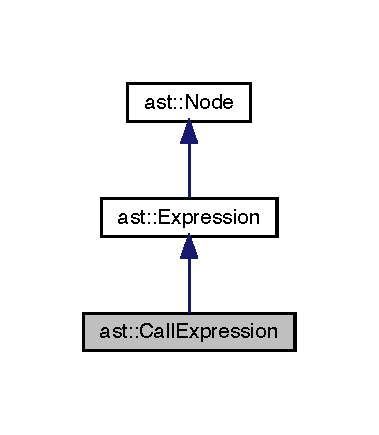
\includegraphics[width=182pt]{structast_1_1_call_expression__inherit__graph}
\end{center}
\end{figure}


Collaboration diagram for ast\+:\+:Call\+Expression\+:
\nopagebreak
\begin{figure}[H]
\begin{center}
\leavevmode
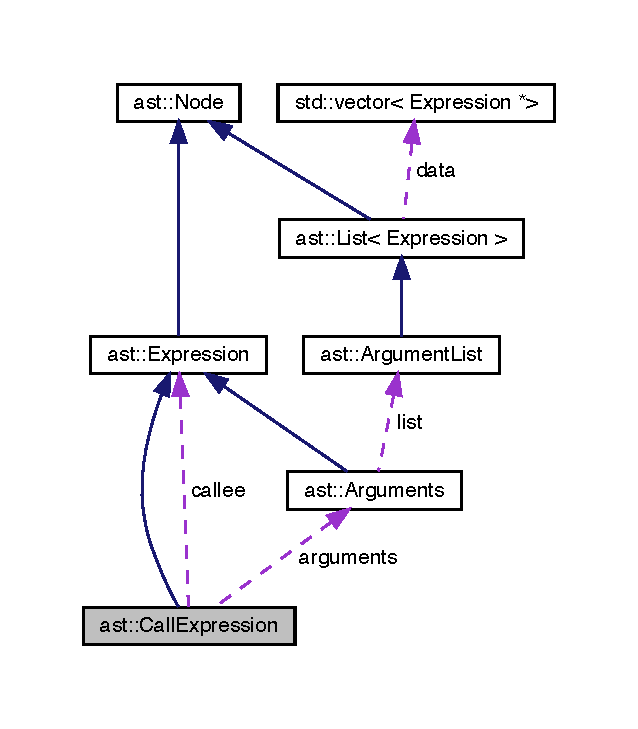
\includegraphics[width=306pt]{structast_1_1_call_expression__coll__graph}
\end{center}
\end{figure}
\subsection*{Public Member Functions}
\begin{DoxyCompactItemize}
\item 
\hyperlink{structast_1_1_call_expression_a4f89b2a241988623c1378a85db795356}{Call\+Expression} (\hyperlink{structast_1_1_expression}{Expression} $\ast$\hyperlink{structast_1_1_call_expression_a6b944439ac86b3d9a8bf984be9a213b9}{callee}, \hyperlink{structast_1_1_arguments}{Arguments} $\ast$\hyperlink{structast_1_1_call_expression_a733b720a818f5c75f2ea96e40360a6ba}{arguments}=nullptr)
\item 
void \hyperlink{structast_1_1_call_expression_abc165321a5ce18456ae0eb51541a4b7e}{accept} (\hyperlink{structast_1_1_visitor}{Visitor} \&visitor) const override
\end{DoxyCompactItemize}
\subsection*{Public Attributes}
\begin{DoxyCompactItemize}
\item 
\hyperlink{structast_1_1_expression}{Expression} $\ast$ \hyperlink{structast_1_1_call_expression_a6b944439ac86b3d9a8bf984be9a213b9}{callee}
\item 
\hyperlink{structast_1_1_arguments}{Arguments} $\ast$ \hyperlink{structast_1_1_call_expression_a733b720a818f5c75f2ea96e40360a6ba}{arguments}
\end{DoxyCompactItemize}


\subsection{Constructor \& Destructor Documentation}
\mbox{\Hypertarget{structast_1_1_call_expression_a4f89b2a241988623c1378a85db795356}\label{structast_1_1_call_expression_a4f89b2a241988623c1378a85db795356}} 
\index{ast\+::\+Call\+Expression@{ast\+::\+Call\+Expression}!Call\+Expression@{Call\+Expression}}
\index{Call\+Expression@{Call\+Expression}!ast\+::\+Call\+Expression@{ast\+::\+Call\+Expression}}
\subsubsection{\texorpdfstring{Call\+Expression()}{CallExpression()}}
{\footnotesize\ttfamily ast\+::\+Call\+Expression\+::\+Call\+Expression (\begin{DoxyParamCaption}\item[{\hyperlink{structast_1_1_expression}{Expression} $\ast$}]{callee,  }\item[{\hyperlink{structast_1_1_arguments}{Arguments} $\ast$}]{arguments = {\ttfamily nullptr} }\end{DoxyParamCaption})\hspace{0.3cm}{\ttfamily [inline]}}



\subsection{Member Function Documentation}
\mbox{\Hypertarget{structast_1_1_call_expression_abc165321a5ce18456ae0eb51541a4b7e}\label{structast_1_1_call_expression_abc165321a5ce18456ae0eb51541a4b7e}} 
\index{ast\+::\+Call\+Expression@{ast\+::\+Call\+Expression}!accept@{accept}}
\index{accept@{accept}!ast\+::\+Call\+Expression@{ast\+::\+Call\+Expression}}
\subsubsection{\texorpdfstring{accept()}{accept()}}
{\footnotesize\ttfamily void ast\+::\+Call\+Expression\+::accept (\begin{DoxyParamCaption}\item[{\hyperlink{structast_1_1_visitor}{Visitor} \&}]{visitor }\end{DoxyParamCaption}) const\hspace{0.3cm}{\ttfamily [inline]}, {\ttfamily [override]}, {\ttfamily [virtual]}}



Implements \hyperlink{structast_1_1_node_abc089ee6caaf06a4445ebdd8391fdebc}{ast\+::\+Node}.



\subsection{Member Data Documentation}
\mbox{\Hypertarget{structast_1_1_call_expression_a733b720a818f5c75f2ea96e40360a6ba}\label{structast_1_1_call_expression_a733b720a818f5c75f2ea96e40360a6ba}} 
\index{ast\+::\+Call\+Expression@{ast\+::\+Call\+Expression}!arguments@{arguments}}
\index{arguments@{arguments}!ast\+::\+Call\+Expression@{ast\+::\+Call\+Expression}}
\subsubsection{\texorpdfstring{arguments}{arguments}}
{\footnotesize\ttfamily \hyperlink{structast_1_1_arguments}{Arguments}$\ast$ ast\+::\+Call\+Expression\+::arguments}

\mbox{\Hypertarget{structast_1_1_call_expression_a6b944439ac86b3d9a8bf984be9a213b9}\label{structast_1_1_call_expression_a6b944439ac86b3d9a8bf984be9a213b9}} 
\index{ast\+::\+Call\+Expression@{ast\+::\+Call\+Expression}!callee@{callee}}
\index{callee@{callee}!ast\+::\+Call\+Expression@{ast\+::\+Call\+Expression}}
\subsubsection{\texorpdfstring{callee}{callee}}
{\footnotesize\ttfamily \hyperlink{structast_1_1_expression}{Expression}$\ast$ ast\+::\+Call\+Expression\+::callee}



The documentation for this struct was generated from the following file\+:\begin{DoxyCompactItemize}
\item 
src/\hyperlink{ast_8h}{ast.\+h}\end{DoxyCompactItemize}

\hypertarget{structast_1_1_case_block}{}\section{ast\+:\+:Case\+Block Struct Reference}
\label{structast_1_1_case_block}\index{ast\+::\+Case\+Block@{ast\+::\+Case\+Block}}


{\ttfamily \#include $<$ast.\+h$>$}



Inheritance diagram for ast\+:\+:Case\+Block\+:
\nopagebreak
\begin{figure}[H]
\begin{center}
\leavevmode
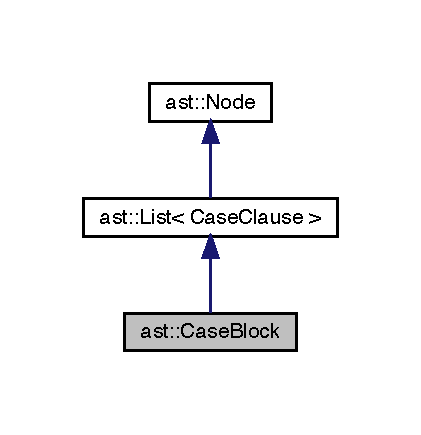
\includegraphics[width=202pt]{structast_1_1_case_block__inherit__graph}
\end{center}
\end{figure}


Collaboration diagram for ast\+:\+:Case\+Block\+:
\nopagebreak
\begin{figure}[H]
\begin{center}
\leavevmode
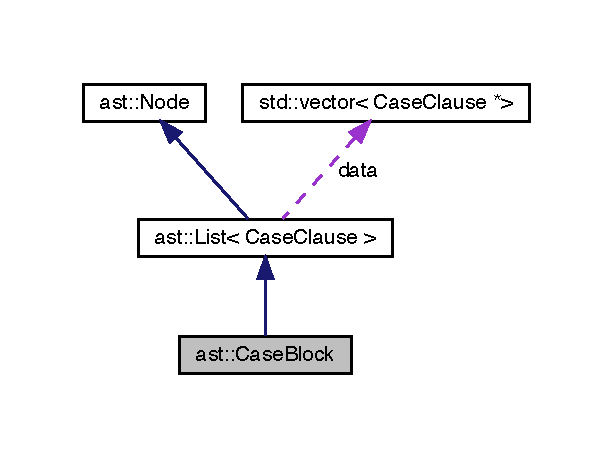
\includegraphics[width=294pt]{structast_1_1_case_block__coll__graph}
\end{center}
\end{figure}
\subsection*{Additional Inherited Members}


The documentation for this struct was generated from the following file\+:\begin{DoxyCompactItemize}
\item 
src/\hyperlink{ast_8h}{ast.\+h}\end{DoxyCompactItemize}

\hypertarget{structast_1_1_case_clause}{}\section{ast\+:\+:Case\+Clause Struct Reference}
\label{structast_1_1_case_clause}\index{ast\+::\+Case\+Clause@{ast\+::\+Case\+Clause}}


{\ttfamily \#include $<$ast.\+h$>$}



Inheritance diagram for ast\+:\+:Case\+Clause\+:
\nopagebreak
\begin{figure}[H]
\begin{center}
\leavevmode
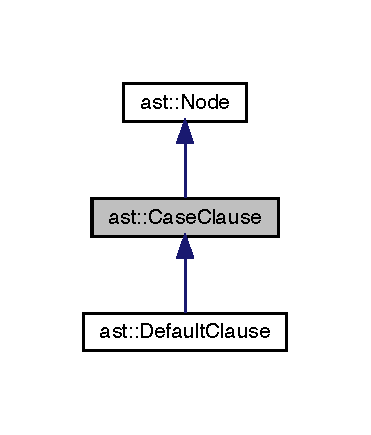
\includegraphics[width=178pt]{structast_1_1_case_clause__inherit__graph}
\end{center}
\end{figure}


Collaboration diagram for ast\+:\+:Case\+Clause\+:
\nopagebreak
\begin{figure}[H]
\begin{center}
\leavevmode
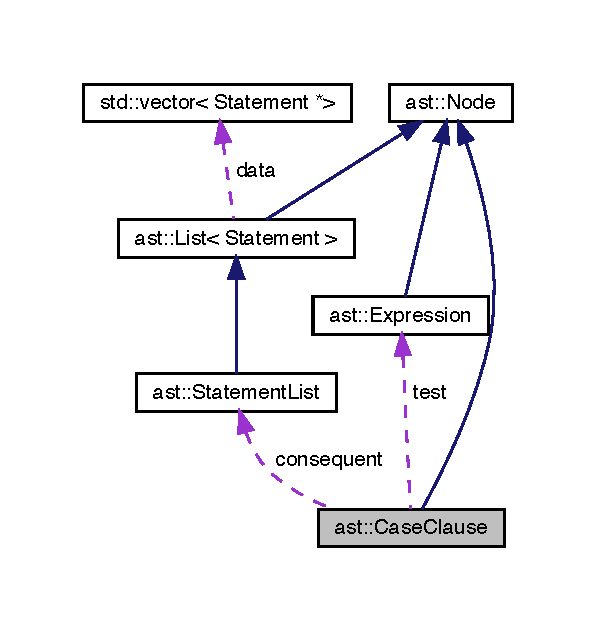
\includegraphics[width=286pt]{structast_1_1_case_clause__coll__graph}
\end{center}
\end{figure}
\subsection*{Public Member Functions}
\begin{DoxyCompactItemize}
\item 
\hyperlink{structast_1_1_case_clause_a9f9501a1d6e46037478537f54e1a1cfa}{Case\+Clause} (\hyperlink{structast_1_1_expression}{Expression} $\ast$\hyperlink{structast_1_1_case_clause_aee3633f283d925ec229674d09970b4b9}{test}, \hyperlink{structast_1_1_statement_list}{Statement\+List} $\ast$\hyperlink{structast_1_1_case_clause_ad858f522c59ec1fe025067c1799df288}{consequent})
\item 
void \hyperlink{structast_1_1_case_clause_a070bb52dc711dc7272ab8d2496631723}{accept} (\hyperlink{structast_1_1_visitor}{Visitor} \&visitor) const override
\end{DoxyCompactItemize}
\subsection*{Public Attributes}
\begin{DoxyCompactItemize}
\item 
\hyperlink{structast_1_1_expression}{Expression} $\ast$ \hyperlink{structast_1_1_case_clause_aee3633f283d925ec229674d09970b4b9}{test}
\item 
\hyperlink{structast_1_1_statement_list}{Statement\+List} $\ast$ \hyperlink{structast_1_1_case_clause_ad858f522c59ec1fe025067c1799df288}{consequent}
\end{DoxyCompactItemize}


\subsection{Constructor \& Destructor Documentation}
\mbox{\Hypertarget{structast_1_1_case_clause_a9f9501a1d6e46037478537f54e1a1cfa}\label{structast_1_1_case_clause_a9f9501a1d6e46037478537f54e1a1cfa}} 
\index{ast\+::\+Case\+Clause@{ast\+::\+Case\+Clause}!Case\+Clause@{Case\+Clause}}
\index{Case\+Clause@{Case\+Clause}!ast\+::\+Case\+Clause@{ast\+::\+Case\+Clause}}
\subsubsection{\texorpdfstring{Case\+Clause()}{CaseClause()}}
{\footnotesize\ttfamily ast\+::\+Case\+Clause\+::\+Case\+Clause (\begin{DoxyParamCaption}\item[{\hyperlink{structast_1_1_expression}{Expression} $\ast$}]{test,  }\item[{\hyperlink{structast_1_1_statement_list}{Statement\+List} $\ast$}]{consequent }\end{DoxyParamCaption})\hspace{0.3cm}{\ttfamily [inline]}}



\subsection{Member Function Documentation}
\mbox{\Hypertarget{structast_1_1_case_clause_a070bb52dc711dc7272ab8d2496631723}\label{structast_1_1_case_clause_a070bb52dc711dc7272ab8d2496631723}} 
\index{ast\+::\+Case\+Clause@{ast\+::\+Case\+Clause}!accept@{accept}}
\index{accept@{accept}!ast\+::\+Case\+Clause@{ast\+::\+Case\+Clause}}
\subsubsection{\texorpdfstring{accept()}{accept()}}
{\footnotesize\ttfamily void ast\+::\+Case\+Clause\+::accept (\begin{DoxyParamCaption}\item[{\hyperlink{structast_1_1_visitor}{Visitor} \&}]{visitor }\end{DoxyParamCaption}) const\hspace{0.3cm}{\ttfamily [inline]}, {\ttfamily [override]}, {\ttfamily [virtual]}}



Implements \hyperlink{structast_1_1_node_abc089ee6caaf06a4445ebdd8391fdebc}{ast\+::\+Node}.



Reimplemented in \hyperlink{structast_1_1_default_clause_a9a96288d67e4e058c860d094f6a5e3a8}{ast\+::\+Default\+Clause}.



\subsection{Member Data Documentation}
\mbox{\Hypertarget{structast_1_1_case_clause_ad858f522c59ec1fe025067c1799df288}\label{structast_1_1_case_clause_ad858f522c59ec1fe025067c1799df288}} 
\index{ast\+::\+Case\+Clause@{ast\+::\+Case\+Clause}!consequent@{consequent}}
\index{consequent@{consequent}!ast\+::\+Case\+Clause@{ast\+::\+Case\+Clause}}
\subsubsection{\texorpdfstring{consequent}{consequent}}
{\footnotesize\ttfamily \hyperlink{structast_1_1_statement_list}{Statement\+List}$\ast$ ast\+::\+Case\+Clause\+::consequent}

\mbox{\Hypertarget{structast_1_1_case_clause_aee3633f283d925ec229674d09970b4b9}\label{structast_1_1_case_clause_aee3633f283d925ec229674d09970b4b9}} 
\index{ast\+::\+Case\+Clause@{ast\+::\+Case\+Clause}!test@{test}}
\index{test@{test}!ast\+::\+Case\+Clause@{ast\+::\+Case\+Clause}}
\subsubsection{\texorpdfstring{test}{test}}
{\footnotesize\ttfamily \hyperlink{structast_1_1_expression}{Expression}$\ast$ ast\+::\+Case\+Clause\+::test}



The documentation for this struct was generated from the following file\+:\begin{DoxyCompactItemize}
\item 
src/\hyperlink{ast_8h}{ast.\+h}\end{DoxyCompactItemize}

\hypertarget{structast_1_1_conditional_expression}{}\section{ast\+:\+:Conditional\+Expression Struct Reference}
\label{structast_1_1_conditional_expression}\index{ast\+::\+Conditional\+Expression@{ast\+::\+Conditional\+Expression}}


{\ttfamily \#include $<$ast.\+h$>$}



Inheritance diagram for ast\+:\+:Conditional\+Expression\+:
\nopagebreak
\begin{figure}[H]
\begin{center}
\leavevmode
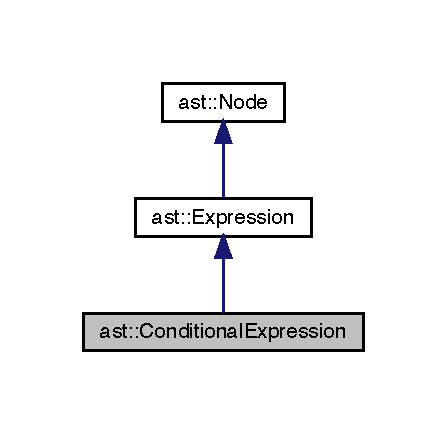
\includegraphics[width=214pt]{structast_1_1_conditional_expression__inherit__graph}
\end{center}
\end{figure}


Collaboration diagram for ast\+:\+:Conditional\+Expression\+:
\nopagebreak
\begin{figure}[H]
\begin{center}
\leavevmode
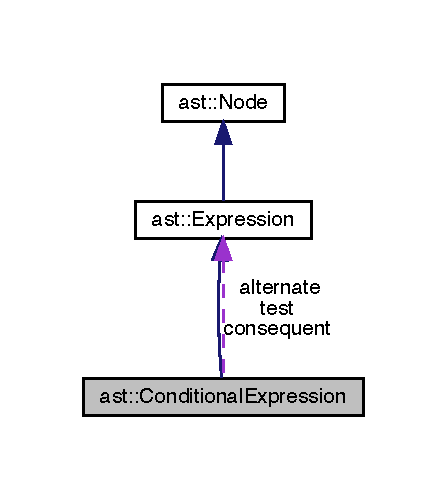
\includegraphics[width=214pt]{structast_1_1_conditional_expression__coll__graph}
\end{center}
\end{figure}
\subsection*{Public Member Functions}
\begin{DoxyCompactItemize}
\item 
\hyperlink{structast_1_1_conditional_expression_ae1d0b0d1bdff64be72a8c506a7ed05f2}{Conditional\+Expression} (\hyperlink{structast_1_1_expression}{Expression} $\ast$\hyperlink{structast_1_1_conditional_expression_ae45a4e413943196c548657c3259dafa5}{test}, \hyperlink{structast_1_1_expression}{Expression} $\ast$\hyperlink{structast_1_1_conditional_expression_a156bf0acbb9f51a660cd8270fd5fceea}{consequent}, \hyperlink{structast_1_1_expression}{Expression} $\ast$\hyperlink{structast_1_1_conditional_expression_a26b4ef799945f3670e759c4d396b3fb2}{alternate})
\item 
void \hyperlink{structast_1_1_conditional_expression_a97fb13e04440b153cc6c1ded95b35e40}{accept} (\hyperlink{structast_1_1_visitor}{Visitor} \&visitor) const override
\end{DoxyCompactItemize}
\subsection*{Public Attributes}
\begin{DoxyCompactItemize}
\item 
\hyperlink{structast_1_1_expression}{Expression} $\ast$ \hyperlink{structast_1_1_conditional_expression_ae45a4e413943196c548657c3259dafa5}{test}
\item 
\hyperlink{structast_1_1_expression}{Expression} $\ast$ \hyperlink{structast_1_1_conditional_expression_a156bf0acbb9f51a660cd8270fd5fceea}{consequent}
\item 
\hyperlink{structast_1_1_expression}{Expression} $\ast$ \hyperlink{structast_1_1_conditional_expression_a26b4ef799945f3670e759c4d396b3fb2}{alternate}
\end{DoxyCompactItemize}


\subsection{Constructor \& Destructor Documentation}
\mbox{\Hypertarget{structast_1_1_conditional_expression_ae1d0b0d1bdff64be72a8c506a7ed05f2}\label{structast_1_1_conditional_expression_ae1d0b0d1bdff64be72a8c506a7ed05f2}} 
\index{ast\+::\+Conditional\+Expression@{ast\+::\+Conditional\+Expression}!Conditional\+Expression@{Conditional\+Expression}}
\index{Conditional\+Expression@{Conditional\+Expression}!ast\+::\+Conditional\+Expression@{ast\+::\+Conditional\+Expression}}
\subsubsection{\texorpdfstring{Conditional\+Expression()}{ConditionalExpression()}}
{\footnotesize\ttfamily ast\+::\+Conditional\+Expression\+::\+Conditional\+Expression (\begin{DoxyParamCaption}\item[{\hyperlink{structast_1_1_expression}{Expression} $\ast$}]{test,  }\item[{\hyperlink{structast_1_1_expression}{Expression} $\ast$}]{consequent,  }\item[{\hyperlink{structast_1_1_expression}{Expression} $\ast$}]{alternate }\end{DoxyParamCaption})\hspace{0.3cm}{\ttfamily [inline]}}



\subsection{Member Function Documentation}
\mbox{\Hypertarget{structast_1_1_conditional_expression_a97fb13e04440b153cc6c1ded95b35e40}\label{structast_1_1_conditional_expression_a97fb13e04440b153cc6c1ded95b35e40}} 
\index{ast\+::\+Conditional\+Expression@{ast\+::\+Conditional\+Expression}!accept@{accept}}
\index{accept@{accept}!ast\+::\+Conditional\+Expression@{ast\+::\+Conditional\+Expression}}
\subsubsection{\texorpdfstring{accept()}{accept()}}
{\footnotesize\ttfamily void ast\+::\+Conditional\+Expression\+::accept (\begin{DoxyParamCaption}\item[{\hyperlink{structast_1_1_visitor}{Visitor} \&}]{visitor }\end{DoxyParamCaption}) const\hspace{0.3cm}{\ttfamily [inline]}, {\ttfamily [override]}, {\ttfamily [virtual]}}



Implements \hyperlink{structast_1_1_node_abc089ee6caaf06a4445ebdd8391fdebc}{ast\+::\+Node}.



\subsection{Member Data Documentation}
\mbox{\Hypertarget{structast_1_1_conditional_expression_a26b4ef799945f3670e759c4d396b3fb2}\label{structast_1_1_conditional_expression_a26b4ef799945f3670e759c4d396b3fb2}} 
\index{ast\+::\+Conditional\+Expression@{ast\+::\+Conditional\+Expression}!alternate@{alternate}}
\index{alternate@{alternate}!ast\+::\+Conditional\+Expression@{ast\+::\+Conditional\+Expression}}
\subsubsection{\texorpdfstring{alternate}{alternate}}
{\footnotesize\ttfamily \hyperlink{structast_1_1_expression}{Expression}$\ast$ ast\+::\+Conditional\+Expression\+::alternate}

\mbox{\Hypertarget{structast_1_1_conditional_expression_a156bf0acbb9f51a660cd8270fd5fceea}\label{structast_1_1_conditional_expression_a156bf0acbb9f51a660cd8270fd5fceea}} 
\index{ast\+::\+Conditional\+Expression@{ast\+::\+Conditional\+Expression}!consequent@{consequent}}
\index{consequent@{consequent}!ast\+::\+Conditional\+Expression@{ast\+::\+Conditional\+Expression}}
\subsubsection{\texorpdfstring{consequent}{consequent}}
{\footnotesize\ttfamily \hyperlink{structast_1_1_expression}{Expression}$\ast$ ast\+::\+Conditional\+Expression\+::consequent}

\mbox{\Hypertarget{structast_1_1_conditional_expression_ae45a4e413943196c548657c3259dafa5}\label{structast_1_1_conditional_expression_ae45a4e413943196c548657c3259dafa5}} 
\index{ast\+::\+Conditional\+Expression@{ast\+::\+Conditional\+Expression}!test@{test}}
\index{test@{test}!ast\+::\+Conditional\+Expression@{ast\+::\+Conditional\+Expression}}
\subsubsection{\texorpdfstring{test}{test}}
{\footnotesize\ttfamily \hyperlink{structast_1_1_expression}{Expression}$\ast$ ast\+::\+Conditional\+Expression\+::test}



The documentation for this struct was generated from the following file\+:\begin{DoxyCompactItemize}
\item 
src/\hyperlink{ast_8h}{ast.\+h}\end{DoxyCompactItemize}

\hypertarget{structast_1_1_continue_statement}{}\section{ast\+:\+:Continue\+Statement Struct Reference}
\label{structast_1_1_continue_statement}\index{ast\+::\+Continue\+Statement@{ast\+::\+Continue\+Statement}}


{\ttfamily \#include $<$ast.\+h$>$}



Inheritance diagram for ast\+:\+:Continue\+Statement\+:\nopagebreak
\begin{figure}[H]
\begin{center}
\leavevmode
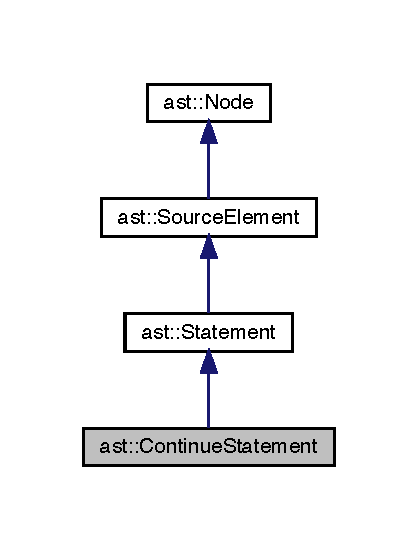
\includegraphics[width=201pt]{structast_1_1_continue_statement__inherit__graph}
\end{center}
\end{figure}


Collaboration diagram for ast\+:\+:Continue\+Statement\+:
\nopagebreak
\begin{figure}[H]
\begin{center}
\leavevmode
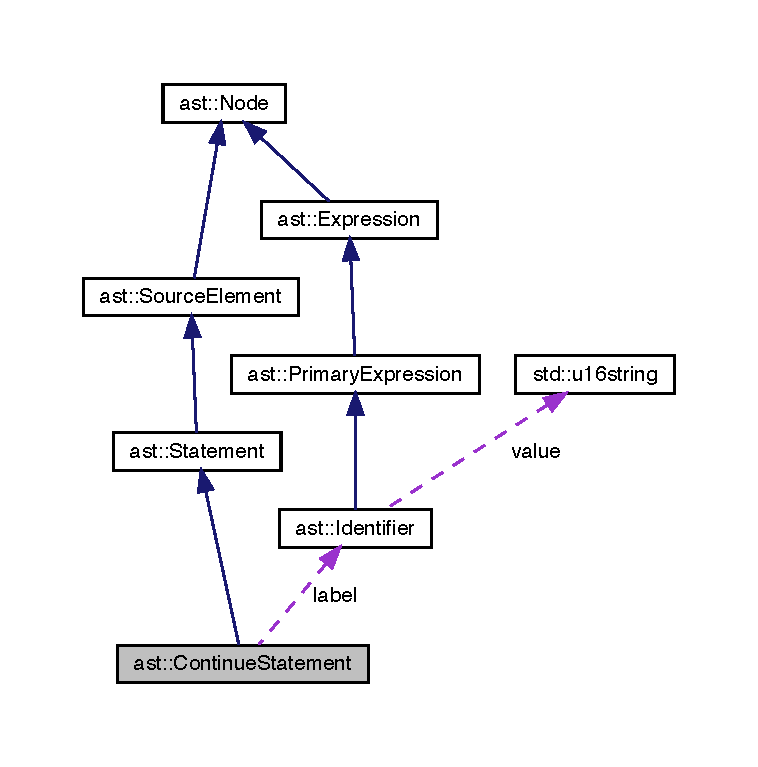
\includegraphics[width=350pt]{structast_1_1_continue_statement__coll__graph}
\end{center}
\end{figure}
\subsection*{Public Member Functions}
\begin{DoxyCompactItemize}
\item 
\hyperlink{structast_1_1_continue_statement_a59aae4f17cdf011db49ae621a7a278f4}{Continue\+Statement} (\hyperlink{structast_1_1_identifier}{Identifier} $\ast$\hyperlink{structast_1_1_continue_statement_ad9bea443914e61a2f69861d7f45e17bc}{label}=nullptr)
\item 
void \hyperlink{structast_1_1_continue_statement_a60101cc01b95c4fab4edb2adf7cb70f3}{accept} (\hyperlink{structast_1_1_visitor}{Visitor} \&visitor) const override
\end{DoxyCompactItemize}
\subsection*{Public Attributes}
\begin{DoxyCompactItemize}
\item 
\hyperlink{structast_1_1_identifier}{Identifier} $\ast$ \hyperlink{structast_1_1_continue_statement_ad9bea443914e61a2f69861d7f45e17bc}{label}
\end{DoxyCompactItemize}


\subsection{Constructor \& Destructor Documentation}
\mbox{\Hypertarget{structast_1_1_continue_statement_a59aae4f17cdf011db49ae621a7a278f4}\label{structast_1_1_continue_statement_a59aae4f17cdf011db49ae621a7a278f4}} 
\index{ast\+::\+Continue\+Statement@{ast\+::\+Continue\+Statement}!Continue\+Statement@{Continue\+Statement}}
\index{Continue\+Statement@{Continue\+Statement}!ast\+::\+Continue\+Statement@{ast\+::\+Continue\+Statement}}
\subsubsection{\texorpdfstring{Continue\+Statement()}{ContinueStatement()}}
{\footnotesize\ttfamily ast\+::\+Continue\+Statement\+::\+Continue\+Statement (\begin{DoxyParamCaption}\item[{\hyperlink{structast_1_1_identifier}{Identifier} $\ast$}]{label = {\ttfamily nullptr} }\end{DoxyParamCaption})\hspace{0.3cm}{\ttfamily [inline]}}



\subsection{Member Function Documentation}
\mbox{\Hypertarget{structast_1_1_continue_statement_a60101cc01b95c4fab4edb2adf7cb70f3}\label{structast_1_1_continue_statement_a60101cc01b95c4fab4edb2adf7cb70f3}} 
\index{ast\+::\+Continue\+Statement@{ast\+::\+Continue\+Statement}!accept@{accept}}
\index{accept@{accept}!ast\+::\+Continue\+Statement@{ast\+::\+Continue\+Statement}}
\subsubsection{\texorpdfstring{accept()}{accept()}}
{\footnotesize\ttfamily void ast\+::\+Continue\+Statement\+::accept (\begin{DoxyParamCaption}\item[{\hyperlink{structast_1_1_visitor}{Visitor} \&}]{visitor }\end{DoxyParamCaption}) const\hspace{0.3cm}{\ttfamily [inline]}, {\ttfamily [override]}, {\ttfamily [virtual]}}



Implements \hyperlink{structast_1_1_node_abc089ee6caaf06a4445ebdd8391fdebc}{ast\+::\+Node}.



\subsection{Member Data Documentation}
\mbox{\Hypertarget{structast_1_1_continue_statement_ad9bea443914e61a2f69861d7f45e17bc}\label{structast_1_1_continue_statement_ad9bea443914e61a2f69861d7f45e17bc}} 
\index{ast\+::\+Continue\+Statement@{ast\+::\+Continue\+Statement}!label@{label}}
\index{label@{label}!ast\+::\+Continue\+Statement@{ast\+::\+Continue\+Statement}}
\subsubsection{\texorpdfstring{label}{label}}
{\footnotesize\ttfamily \hyperlink{structast_1_1_identifier}{Identifier}$\ast$ ast\+::\+Continue\+Statement\+::label}



The documentation for this struct was generated from the following file\+:\begin{DoxyCompactItemize}
\item 
src/\hyperlink{ast_8h}{ast.\+h}\end{DoxyCompactItemize}

\hypertarget{structast_1_1_debugger_statement}{}\section{ast\+:\+:Debugger\+Statement Struct Reference}
\label{structast_1_1_debugger_statement}\index{ast\+::\+Debugger\+Statement@{ast\+::\+Debugger\+Statement}}


{\ttfamily \#include $<$ast.\+h$>$}



Inheritance diagram for ast\+:\+:Debugger\+Statement\+:\nopagebreak
\begin{figure}[H]
\begin{center}
\leavevmode
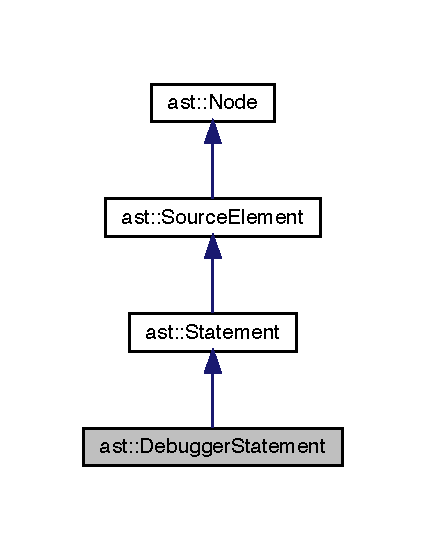
\includegraphics[width=204pt]{structast_1_1_debugger_statement__inherit__graph}
\end{center}
\end{figure}


Collaboration diagram for ast\+:\+:Debugger\+Statement\+:\nopagebreak
\begin{figure}[H]
\begin{center}
\leavevmode
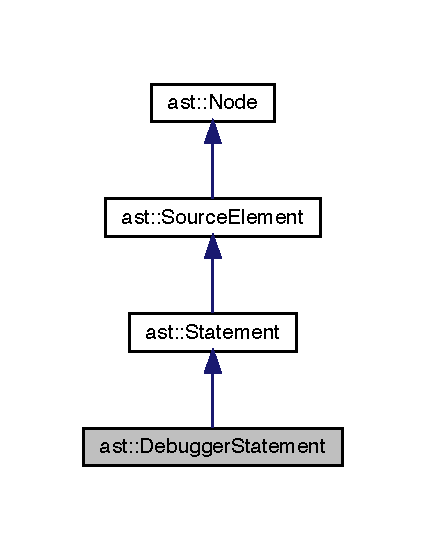
\includegraphics[width=204pt]{structast_1_1_debugger_statement__coll__graph}
\end{center}
\end{figure}
\subsection*{Public Member Functions}
\begin{DoxyCompactItemize}
\item 
void \hyperlink{structast_1_1_debugger_statement_a804fde650cdb57afd2c11b8f466f3af0}{accept} (\hyperlink{structast_1_1_visitor}{Visitor} \&visitor) const override
\end{DoxyCompactItemize}


\subsection{Member Function Documentation}
\mbox{\Hypertarget{structast_1_1_debugger_statement_a804fde650cdb57afd2c11b8f466f3af0}\label{structast_1_1_debugger_statement_a804fde650cdb57afd2c11b8f466f3af0}} 
\index{ast\+::\+Debugger\+Statement@{ast\+::\+Debugger\+Statement}!accept@{accept}}
\index{accept@{accept}!ast\+::\+Debugger\+Statement@{ast\+::\+Debugger\+Statement}}
\subsubsection{\texorpdfstring{accept()}{accept()}}
{\footnotesize\ttfamily void ast\+::\+Debugger\+Statement\+::accept (\begin{DoxyParamCaption}\item[{\hyperlink{structast_1_1_visitor}{Visitor} \&}]{visitor }\end{DoxyParamCaption}) const\hspace{0.3cm}{\ttfamily [inline]}, {\ttfamily [override]}, {\ttfamily [virtual]}}



Implements \hyperlink{structast_1_1_node_abc089ee6caaf06a4445ebdd8391fdebc}{ast\+::\+Node}.



The documentation for this struct was generated from the following file\+:\begin{DoxyCompactItemize}
\item 
src/\hyperlink{ast_8h}{ast.\+h}\end{DoxyCompactItemize}

\hypertarget{struct_token_1_1_debug_info}{}\section{Token\+:\+:Debug\+Info Struct Reference}
\label{struct_token_1_1_debug_info}\index{Token\+::\+Debug\+Info@{Token\+::\+Debug\+Info}}


{\ttfamily \#include $<$token.\+h$>$}

\subsection*{Public Member Functions}
\begin{DoxyCompactItemize}
\item 
virtual \textbf{ std\+::string} \hyperlink{struct_token_1_1_debug_info_a4d66aa65422c236198bbcc616bba250f}{syntax\+\_\+error\+\_\+at} () const =0
\item 
virtual \textbf{ std\+::string} \hyperlink{struct_token_1_1_debug_info_a0860d9b875240dafa0e00756d27e55bb}{loc} () const =0
\end{DoxyCompactItemize}


\subsection{Member Function Documentation}
\mbox{\Hypertarget{struct_token_1_1_debug_info_a0860d9b875240dafa0e00756d27e55bb}\label{struct_token_1_1_debug_info_a0860d9b875240dafa0e00756d27e55bb}} 
\index{Token\+::\+Debug\+Info@{Token\+::\+Debug\+Info}!loc@{loc}}
\index{loc@{loc}!Token\+::\+Debug\+Info@{Token\+::\+Debug\+Info}}
\subsubsection{\texorpdfstring{loc()}{loc()}}
{\footnotesize\ttfamily virtual \textbf{ std\+::string} Token\+::\+Debug\+Info\+::loc (\begin{DoxyParamCaption}{ }\end{DoxyParamCaption}) const\hspace{0.3cm}{\ttfamily [pure virtual]}}

\mbox{\Hypertarget{struct_token_1_1_debug_info_a4d66aa65422c236198bbcc616bba250f}\label{struct_token_1_1_debug_info_a4d66aa65422c236198bbcc616bba250f}} 
\index{Token\+::\+Debug\+Info@{Token\+::\+Debug\+Info}!syntax\+\_\+error\+\_\+at@{syntax\+\_\+error\+\_\+at}}
\index{syntax\+\_\+error\+\_\+at@{syntax\+\_\+error\+\_\+at}!Token\+::\+Debug\+Info@{Token\+::\+Debug\+Info}}
\subsubsection{\texorpdfstring{syntax\+\_\+error\+\_\+at()}{syntax\_error\_at()}}
{\footnotesize\ttfamily virtual \textbf{ std\+::string} Token\+::\+Debug\+Info\+::syntax\+\_\+error\+\_\+at (\begin{DoxyParamCaption}{ }\end{DoxyParamCaption}) const\hspace{0.3cm}{\ttfamily [pure virtual]}}



The documentation for this struct was generated from the following file\+:\begin{DoxyCompactItemize}
\item 
src/\hyperlink{token_8h}{token.\+h}\end{DoxyCompactItemize}

\hypertarget{structast_1_1_declaration}{}\section{ast\+:\+:Declaration Struct Reference}
\label{structast_1_1_declaration}\index{ast\+::\+Declaration@{ast\+::\+Declaration}}


{\ttfamily \#include $<$ast.\+h$>$}



Inheritance diagram for ast\+:\+:Declaration\+:
\nopagebreak
\begin{figure}[H]
\begin{center}
\leavevmode
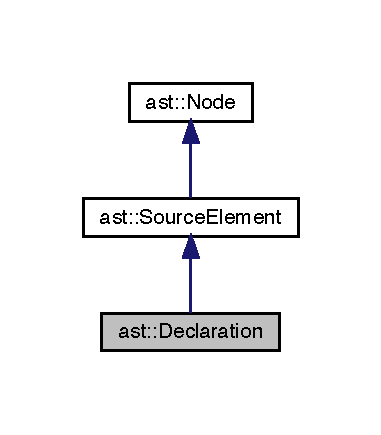
\includegraphics[width=183pt]{structast_1_1_declaration__inherit__graph}
\end{center}
\end{figure}


Collaboration diagram for ast\+:\+:Declaration\+:
\nopagebreak
\begin{figure}[H]
\begin{center}
\leavevmode
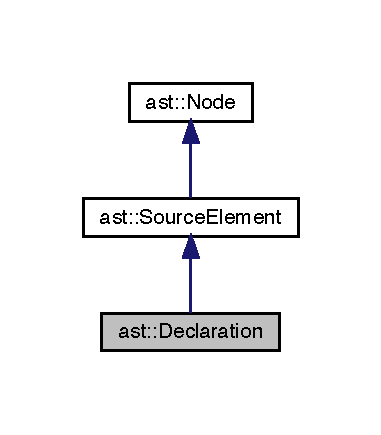
\includegraphics[width=183pt]{structast_1_1_declaration__coll__graph}
\end{center}
\end{figure}
\subsection*{Additional Inherited Members}


The documentation for this struct was generated from the following file\+:\begin{DoxyCompactItemize}
\item 
src/\hyperlink{ast_8h}{ast.\+h}\end{DoxyCompactItemize}

\hypertarget{structast_1_1_default_clause}{}\section{ast\+:\+:Default\+Clause Struct Reference}
\label{structast_1_1_default_clause}\index{ast\+::\+Default\+Clause@{ast\+::\+Default\+Clause}}


{\ttfamily \#include $<$ast.\+h$>$}



Inheritance diagram for ast\+:\+:Default\+Clause\+:
\nopagebreak
\begin{figure}[H]
\begin{center}
\leavevmode
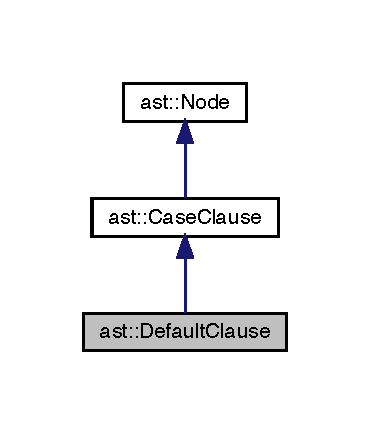
\includegraphics[width=178pt]{structast_1_1_default_clause__inherit__graph}
\end{center}
\end{figure}


Collaboration diagram for ast\+:\+:Default\+Clause\+:
\nopagebreak
\begin{figure}[H]
\begin{center}
\leavevmode
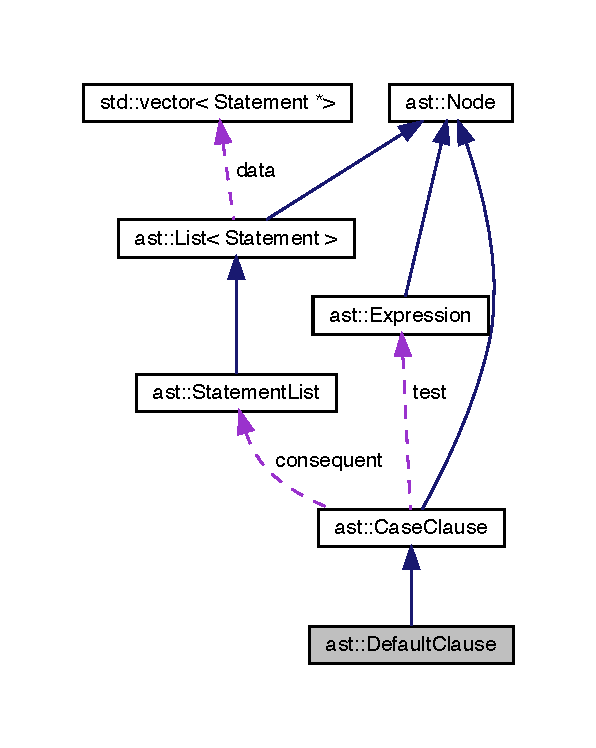
\includegraphics[width=286pt]{structast_1_1_default_clause__coll__graph}
\end{center}
\end{figure}
\subsection*{Public Member Functions}
\begin{DoxyCompactItemize}
\item 
\hyperlink{structast_1_1_default_clause_ae2ed04ca435788a9688223373d14a4d7}{Default\+Clause} (\hyperlink{structast_1_1_statement_list}{Statement\+List} $\ast$\hyperlink{structast_1_1_case_clause_ad858f522c59ec1fe025067c1799df288}{consequent})
\item 
void \hyperlink{structast_1_1_default_clause_a9a96288d67e4e058c860d094f6a5e3a8}{accept} (\hyperlink{structast_1_1_visitor}{Visitor} \&visitor) const override
\end{DoxyCompactItemize}
\subsection*{Additional Inherited Members}


\subsection{Constructor \& Destructor Documentation}
\mbox{\Hypertarget{structast_1_1_default_clause_ae2ed04ca435788a9688223373d14a4d7}\label{structast_1_1_default_clause_ae2ed04ca435788a9688223373d14a4d7}} 
\index{ast\+::\+Default\+Clause@{ast\+::\+Default\+Clause}!Default\+Clause@{Default\+Clause}}
\index{Default\+Clause@{Default\+Clause}!ast\+::\+Default\+Clause@{ast\+::\+Default\+Clause}}
\subsubsection{\texorpdfstring{Default\+Clause()}{DefaultClause()}}
{\footnotesize\ttfamily ast\+::\+Default\+Clause\+::\+Default\+Clause (\begin{DoxyParamCaption}\item[{\hyperlink{structast_1_1_statement_list}{Statement\+List} $\ast$}]{consequent }\end{DoxyParamCaption})\hspace{0.3cm}{\ttfamily [inline]}}



\subsection{Member Function Documentation}
\mbox{\Hypertarget{structast_1_1_default_clause_a9a96288d67e4e058c860d094f6a5e3a8}\label{structast_1_1_default_clause_a9a96288d67e4e058c860d094f6a5e3a8}} 
\index{ast\+::\+Default\+Clause@{ast\+::\+Default\+Clause}!accept@{accept}}
\index{accept@{accept}!ast\+::\+Default\+Clause@{ast\+::\+Default\+Clause}}
\subsubsection{\texorpdfstring{accept()}{accept()}}
{\footnotesize\ttfamily void ast\+::\+Default\+Clause\+::accept (\begin{DoxyParamCaption}\item[{\hyperlink{structast_1_1_visitor}{Visitor} \&}]{visitor }\end{DoxyParamCaption}) const\hspace{0.3cm}{\ttfamily [inline]}, {\ttfamily [override]}, {\ttfamily [virtual]}}



Reimplemented from \hyperlink{structast_1_1_case_clause_a070bb52dc711dc7272ab8d2496631723}{ast\+::\+Case\+Clause}.



The documentation for this struct was generated from the following file\+:\begin{DoxyCompactItemize}
\item 
src/\hyperlink{ast_8h}{ast.\+h}\end{DoxyCompactItemize}

\hypertarget{structast_1_1_do_while_statement}{}\section{ast\+:\+:Do\+While\+Statement Struct Reference}
\label{structast_1_1_do_while_statement}\index{ast\+::\+Do\+While\+Statement@{ast\+::\+Do\+While\+Statement}}


{\ttfamily \#include $<$ast.\+h$>$}



Inheritance diagram for ast\+:\+:Do\+While\+Statement\+:
\nopagebreak
\begin{figure}[H]
\begin{center}
\leavevmode
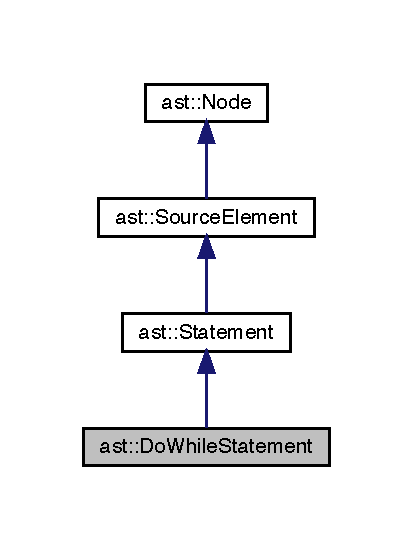
\includegraphics[width=198pt]{structast_1_1_do_while_statement__inherit__graph}
\end{center}
\end{figure}


Collaboration diagram for ast\+:\+:Do\+While\+Statement\+:
\nopagebreak
\begin{figure}[H]
\begin{center}
\leavevmode
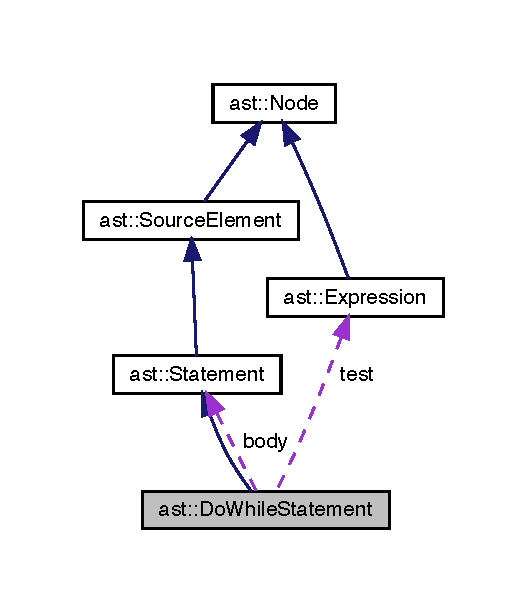
\includegraphics[width=253pt]{structast_1_1_do_while_statement__coll__graph}
\end{center}
\end{figure}
\subsection*{Public Member Functions}
\begin{DoxyCompactItemize}
\item 
void \hyperlink{structast_1_1_do_while_statement_a829cc06274cc0a165e8e274a02a2d373}{accept} (\hyperlink{structast_1_1_visitor}{Visitor} \&visitor) const override
\end{DoxyCompactItemize}
\subsection*{Public Attributes}
\begin{DoxyCompactItemize}
\item 
\hyperlink{structast_1_1_statement}{Statement} $\ast$ \hyperlink{structast_1_1_do_while_statement_a7d1d10fa21fefab6f9ca82a7c88c7986}{body}
\item 
\hyperlink{structast_1_1_expression}{Expression} $\ast$ \hyperlink{structast_1_1_do_while_statement_a9191ed1c7a07db01694873c22e96f32c}{test}
\end{DoxyCompactItemize}


\subsection{Member Function Documentation}
\mbox{\Hypertarget{structast_1_1_do_while_statement_a829cc06274cc0a165e8e274a02a2d373}\label{structast_1_1_do_while_statement_a829cc06274cc0a165e8e274a02a2d373}} 
\index{ast\+::\+Do\+While\+Statement@{ast\+::\+Do\+While\+Statement}!accept@{accept}}
\index{accept@{accept}!ast\+::\+Do\+While\+Statement@{ast\+::\+Do\+While\+Statement}}
\subsubsection{\texorpdfstring{accept()}{accept()}}
{\footnotesize\ttfamily void ast\+::\+Do\+While\+Statement\+::accept (\begin{DoxyParamCaption}\item[{\hyperlink{structast_1_1_visitor}{Visitor} \&}]{visitor }\end{DoxyParamCaption}) const\hspace{0.3cm}{\ttfamily [inline]}, {\ttfamily [override]}, {\ttfamily [virtual]}}



Implements \hyperlink{structast_1_1_node_abc089ee6caaf06a4445ebdd8391fdebc}{ast\+::\+Node}.



\subsection{Member Data Documentation}
\mbox{\Hypertarget{structast_1_1_do_while_statement_a7d1d10fa21fefab6f9ca82a7c88c7986}\label{structast_1_1_do_while_statement_a7d1d10fa21fefab6f9ca82a7c88c7986}} 
\index{ast\+::\+Do\+While\+Statement@{ast\+::\+Do\+While\+Statement}!body@{body}}
\index{body@{body}!ast\+::\+Do\+While\+Statement@{ast\+::\+Do\+While\+Statement}}
\subsubsection{\texorpdfstring{body}{body}}
{\footnotesize\ttfamily \hyperlink{structast_1_1_statement}{Statement}$\ast$ ast\+::\+Do\+While\+Statement\+::body}

\mbox{\Hypertarget{structast_1_1_do_while_statement_a9191ed1c7a07db01694873c22e96f32c}\label{structast_1_1_do_while_statement_a9191ed1c7a07db01694873c22e96f32c}} 
\index{ast\+::\+Do\+While\+Statement@{ast\+::\+Do\+While\+Statement}!test@{test}}
\index{test@{test}!ast\+::\+Do\+While\+Statement@{ast\+::\+Do\+While\+Statement}}
\subsubsection{\texorpdfstring{test}{test}}
{\footnotesize\ttfamily \hyperlink{structast_1_1_expression}{Expression}$\ast$ ast\+::\+Do\+While\+Statement\+::test}



The documentation for this struct was generated from the following file\+:\begin{DoxyCompactItemize}
\item 
src/\hyperlink{ast_8h}{ast.\+h}\end{DoxyCompactItemize}

\hypertarget{structast_1_1_element_list}{}\section{ast\+:\+:Element\+List Struct Reference}
\label{structast_1_1_element_list}\index{ast\+::\+Element\+List@{ast\+::\+Element\+List}}


{\ttfamily \#include $<$ast.\+h$>$}



Inheritance diagram for ast\+:\+:Element\+List\+:
\nopagebreak
\begin{figure}[H]
\begin{center}
\leavevmode
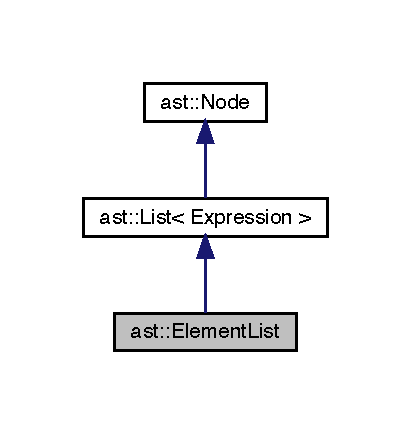
\includegraphics[width=197pt]{structast_1_1_element_list__inherit__graph}
\end{center}
\end{figure}


Collaboration diagram for ast\+:\+:Element\+List\+:
\nopagebreak
\begin{figure}[H]
\begin{center}
\leavevmode
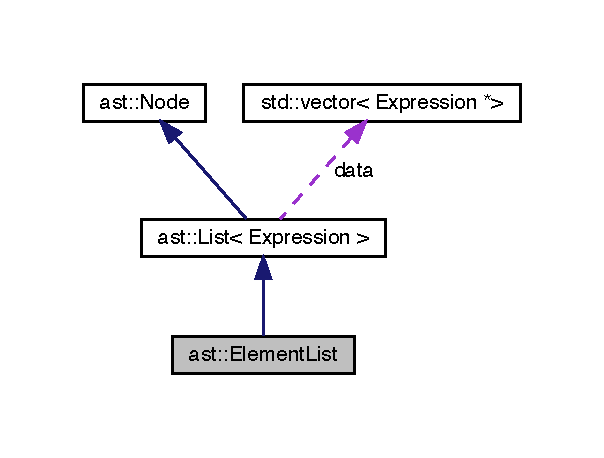
\includegraphics[width=290pt]{structast_1_1_element_list__coll__graph}
\end{center}
\end{figure}
\subsection*{Additional Inherited Members}


The documentation for this struct was generated from the following file\+:\begin{DoxyCompactItemize}
\item 
src/\hyperlink{ast_8h}{ast.\+h}\end{DoxyCompactItemize}

\hypertarget{structast_1_1_elision}{}\section{ast\+:\+:Elision Struct Reference}
\label{structast_1_1_elision}\index{ast\+::\+Elision@{ast\+::\+Elision}}


{\ttfamily \#include $<$ast.\+h$>$}



Inheritance diagram for ast\+:\+:Elision\+:\nopagebreak
\begin{figure}[H]
\begin{center}
\leavevmode
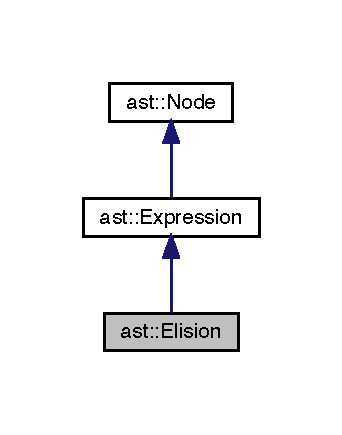
\includegraphics[width=164pt]{structast_1_1_elision__inherit__graph}
\end{center}
\end{figure}


Collaboration diagram for ast\+:\+:Elision\+:\nopagebreak
\begin{figure}[H]
\begin{center}
\leavevmode
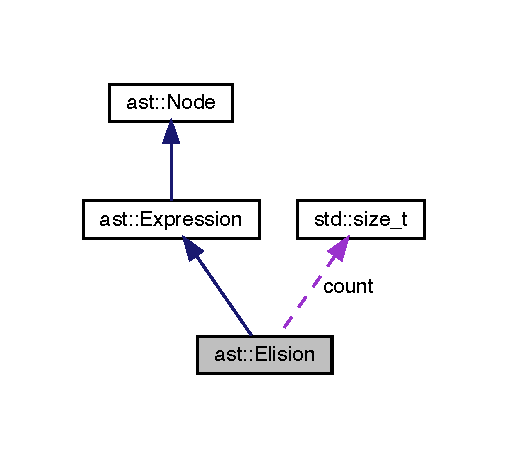
\includegraphics[width=244pt]{structast_1_1_elision__coll__graph}
\end{center}
\end{figure}
\subsection*{Public Member Functions}
\begin{DoxyCompactItemize}
\item 
void \hyperlink{structast_1_1_elision_a6a3fc3746613bdc5228629bf296b50e3}{accept} (\hyperlink{structast_1_1_visitor}{Visitor} \&visitor) const override
\end{DoxyCompactItemize}
\subsection*{Public Attributes}
\begin{DoxyCompactItemize}
\item 
\textbf{ std\+::size\+\_\+t} \hyperlink{structast_1_1_elision_afa81a1129d9ce7f1f59d08a74961ca62}{count} = 1
\end{DoxyCompactItemize}


\subsection{Member Function Documentation}
\mbox{\Hypertarget{structast_1_1_elision_a6a3fc3746613bdc5228629bf296b50e3}\label{structast_1_1_elision_a6a3fc3746613bdc5228629bf296b50e3}} 
\index{ast\+::\+Elision@{ast\+::\+Elision}!accept@{accept}}
\index{accept@{accept}!ast\+::\+Elision@{ast\+::\+Elision}}
\subsubsection{\texorpdfstring{accept()}{accept()}}
{\footnotesize\ttfamily void ast\+::\+Elision\+::accept (\begin{DoxyParamCaption}\item[{\hyperlink{structast_1_1_visitor}{Visitor} \&}]{visitor }\end{DoxyParamCaption}) const\hspace{0.3cm}{\ttfamily [inline]}, {\ttfamily [override]}, {\ttfamily [virtual]}}



Implements \hyperlink{structast_1_1_node_abc089ee6caaf06a4445ebdd8391fdebc}{ast\+::\+Node}.



\subsection{Member Data Documentation}
\mbox{\Hypertarget{structast_1_1_elision_afa81a1129d9ce7f1f59d08a74961ca62}\label{structast_1_1_elision_afa81a1129d9ce7f1f59d08a74961ca62}} 
\index{ast\+::\+Elision@{ast\+::\+Elision}!count@{count}}
\index{count@{count}!ast\+::\+Elision@{ast\+::\+Elision}}
\subsubsection{\texorpdfstring{count}{count}}
{\footnotesize\ttfamily \textbf{ std\+::size\+\_\+t} ast\+::\+Elision\+::count = 1}



The documentation for this struct was generated from the following file\+:\begin{DoxyCompactItemize}
\item 
src/\hyperlink{ast_8h}{ast.\+h}\end{DoxyCompactItemize}

\hypertarget{structast_1_1_empty_statement}{}\section{ast\+:\+:Empty\+Statement Struct Reference}
\label{structast_1_1_empty_statement}\index{ast\+::\+Empty\+Statement@{ast\+::\+Empty\+Statement}}


{\ttfamily \#include $<$ast.\+h$>$}



Inheritance diagram for ast\+:\+:Empty\+Statement\+:\nopagebreak
\begin{figure}[H]
\begin{center}
\leavevmode
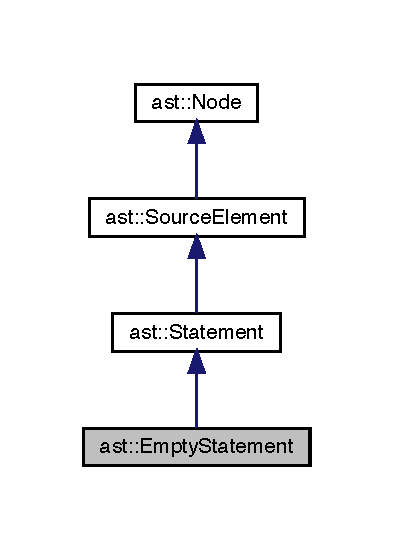
\includegraphics[width=189pt]{structast_1_1_empty_statement__inherit__graph}
\end{center}
\end{figure}


Collaboration diagram for ast\+:\+:Empty\+Statement\+:\nopagebreak
\begin{figure}[H]
\begin{center}
\leavevmode
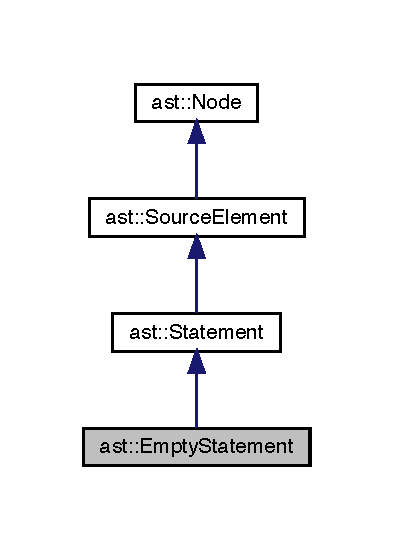
\includegraphics[width=189pt]{structast_1_1_empty_statement__coll__graph}
\end{center}
\end{figure}
\subsection*{Public Member Functions}
\begin{DoxyCompactItemize}
\item 
void \hyperlink{structast_1_1_empty_statement_a32aaa9a97be0d4b6862526a64b5ee6dd}{accept} (\hyperlink{structast_1_1_visitor}{Visitor} \&visitor) const override
\end{DoxyCompactItemize}


\subsection{Member Function Documentation}
\mbox{\Hypertarget{structast_1_1_empty_statement_a32aaa9a97be0d4b6862526a64b5ee6dd}\label{structast_1_1_empty_statement_a32aaa9a97be0d4b6862526a64b5ee6dd}} 
\index{ast\+::\+Empty\+Statement@{ast\+::\+Empty\+Statement}!accept@{accept}}
\index{accept@{accept}!ast\+::\+Empty\+Statement@{ast\+::\+Empty\+Statement}}
\subsubsection{\texorpdfstring{accept()}{accept()}}
{\footnotesize\ttfamily void ast\+::\+Empty\+Statement\+::accept (\begin{DoxyParamCaption}\item[{\hyperlink{structast_1_1_visitor}{Visitor} \&}]{visitor }\end{DoxyParamCaption}) const\hspace{0.3cm}{\ttfamily [inline]}, {\ttfamily [override]}, {\ttfamily [virtual]}}



Implements \hyperlink{structast_1_1_node_abc089ee6caaf06a4445ebdd8391fdebc}{ast\+::\+Node}.



The documentation for this struct was generated from the following file\+:\begin{DoxyCompactItemize}
\item 
src/\hyperlink{ast_8h}{ast.\+h}\end{DoxyCompactItemize}

\hypertarget{struct_token_1_1equal__visitor}{}\section{Token\+:\+:equal\+\_\+visitor Struct Reference}
\label{struct_token_1_1equal__visitor}\index{Token\+::equal\+\_\+visitor@{Token\+::equal\+\_\+visitor}}


Inheritance diagram for Token\+:\+:equal\+\_\+visitor\+:\nopagebreak
\begin{figure}[H]
\begin{center}
\leavevmode
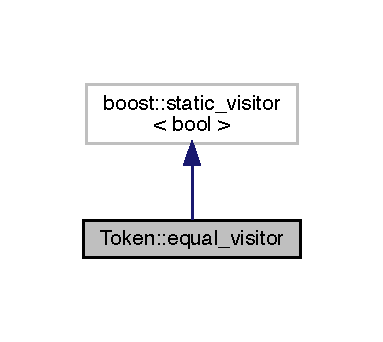
\includegraphics[width=184pt]{struct_token_1_1equal__visitor__inherit__graph}
\end{center}
\end{figure}


Collaboration diagram for Token\+:\+:equal\+\_\+visitor\+:\nopagebreak
\begin{figure}[H]
\begin{center}
\leavevmode
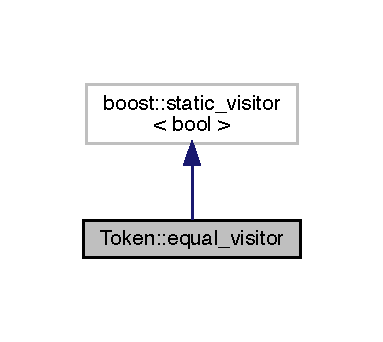
\includegraphics[width=184pt]{struct_token_1_1equal__visitor__coll__graph}
\end{center}
\end{figure}
\subsection*{Public Member Functions}
\begin{DoxyCompactItemize}
\item 
{\footnotesize template$<$typename T $>$ }\\auto \hyperlink{struct_token_1_1equal__visitor_a22bf1a085ca9392c7be2d6a11f07afa5}{operator()} (const T \&lhs, const T \&rhs) const -\/$>$ decltype(lhs.\+value==rhs.\+value, bool())
\item 
bool \hyperlink{struct_token_1_1equal__visitor_a967ea3398b97e8e1af5e52384d5e92f2}{operator()} (const Empty \&, const Empty \&) const
\item 
bool \hyperlink{struct_token_1_1equal__visitor_adcfaf40afbf658dcedcf672c5f94b15d}{operator()} (const Null\+Literal \&, const Null\+Literal \&) const
\item 
{\footnotesize template$<$typename T , typename U $>$ }\\bool \hyperlink{struct_token_1_1equal__visitor_abd104c4e966e4c0e6d43991816f17118}{operator()} (const T \&, const U \&) const
\end{DoxyCompactItemize}


\subsection{Member Function Documentation}
\mbox{\Hypertarget{struct_token_1_1equal__visitor_a22bf1a085ca9392c7be2d6a11f07afa5}\label{struct_token_1_1equal__visitor_a22bf1a085ca9392c7be2d6a11f07afa5}} 
\index{Token\+::equal\+\_\+visitor@{Token\+::equal\+\_\+visitor}!operator()@{operator()}}
\index{operator()@{operator()}!Token\+::equal\+\_\+visitor@{Token\+::equal\+\_\+visitor}}
\subsubsection{\texorpdfstring{operator()()}{operator()()}\hspace{0.1cm}{\footnotesize\ttfamily [1/4]}}
{\footnotesize\ttfamily template$<$typename T $>$ \\
auto Token\+::equal\+\_\+visitor\+::operator() (\begin{DoxyParamCaption}\item[{const T \&}]{lhs,  }\item[{const T \&}]{rhs }\end{DoxyParamCaption}) const -\/$>$ decltype(lhs.\+value == rhs.\+value, bool())
  \hspace{0.3cm}{\ttfamily [inline]}}

\mbox{\Hypertarget{struct_token_1_1equal__visitor_a967ea3398b97e8e1af5e52384d5e92f2}\label{struct_token_1_1equal__visitor_a967ea3398b97e8e1af5e52384d5e92f2}} 
\index{Token\+::equal\+\_\+visitor@{Token\+::equal\+\_\+visitor}!operator()@{operator()}}
\index{operator()@{operator()}!Token\+::equal\+\_\+visitor@{Token\+::equal\+\_\+visitor}}
\subsubsection{\texorpdfstring{operator()()}{operator()()}\hspace{0.1cm}{\footnotesize\ttfamily [2/4]}}
{\footnotesize\ttfamily bool Token\+::equal\+\_\+visitor\+::operator() (\begin{DoxyParamCaption}\item[{const Empty \&}]{,  }\item[{const Empty \&}]{ }\end{DoxyParamCaption}) const\hspace{0.3cm}{\ttfamily [inline]}}

\mbox{\Hypertarget{struct_token_1_1equal__visitor_adcfaf40afbf658dcedcf672c5f94b15d}\label{struct_token_1_1equal__visitor_adcfaf40afbf658dcedcf672c5f94b15d}} 
\index{Token\+::equal\+\_\+visitor@{Token\+::equal\+\_\+visitor}!operator()@{operator()}}
\index{operator()@{operator()}!Token\+::equal\+\_\+visitor@{Token\+::equal\+\_\+visitor}}
\subsubsection{\texorpdfstring{operator()()}{operator()()}\hspace{0.1cm}{\footnotesize\ttfamily [3/4]}}
{\footnotesize\ttfamily bool Token\+::equal\+\_\+visitor\+::operator() (\begin{DoxyParamCaption}\item[{const Null\+Literal \&}]{,  }\item[{const Null\+Literal \&}]{ }\end{DoxyParamCaption}) const\hspace{0.3cm}{\ttfamily [inline]}}

\mbox{\Hypertarget{struct_token_1_1equal__visitor_abd104c4e966e4c0e6d43991816f17118}\label{struct_token_1_1equal__visitor_abd104c4e966e4c0e6d43991816f17118}} 
\index{Token\+::equal\+\_\+visitor@{Token\+::equal\+\_\+visitor}!operator()@{operator()}}
\index{operator()@{operator()}!Token\+::equal\+\_\+visitor@{Token\+::equal\+\_\+visitor}}
\subsubsection{\texorpdfstring{operator()()}{operator()()}\hspace{0.1cm}{\footnotesize\ttfamily [4/4]}}
{\footnotesize\ttfamily template$<$typename T , typename U $>$ \\
bool Token\+::equal\+\_\+visitor\+::operator() (\begin{DoxyParamCaption}\item[{const T \&}]{,  }\item[{const U \&}]{ }\end{DoxyParamCaption}) const\hspace{0.3cm}{\ttfamily [inline]}}



The documentation for this struct was generated from the following file\+:\begin{DoxyCompactItemize}
\item 
src/\hyperlink{token_8cpp}{token.\+cpp}\end{DoxyCompactItemize}

\hypertarget{structast_1_1_expression}{}\section{ast\+:\+:Expression Struct Reference}
\label{structast_1_1_expression}\index{ast\+::\+Expression@{ast\+::\+Expression}}


{\ttfamily \#include $<$ast.\+h$>$}



Inheritance diagram for ast\+:\+:Expression\+:\nopagebreak
\begin{figure}[H]
\begin{center}
\leavevmode
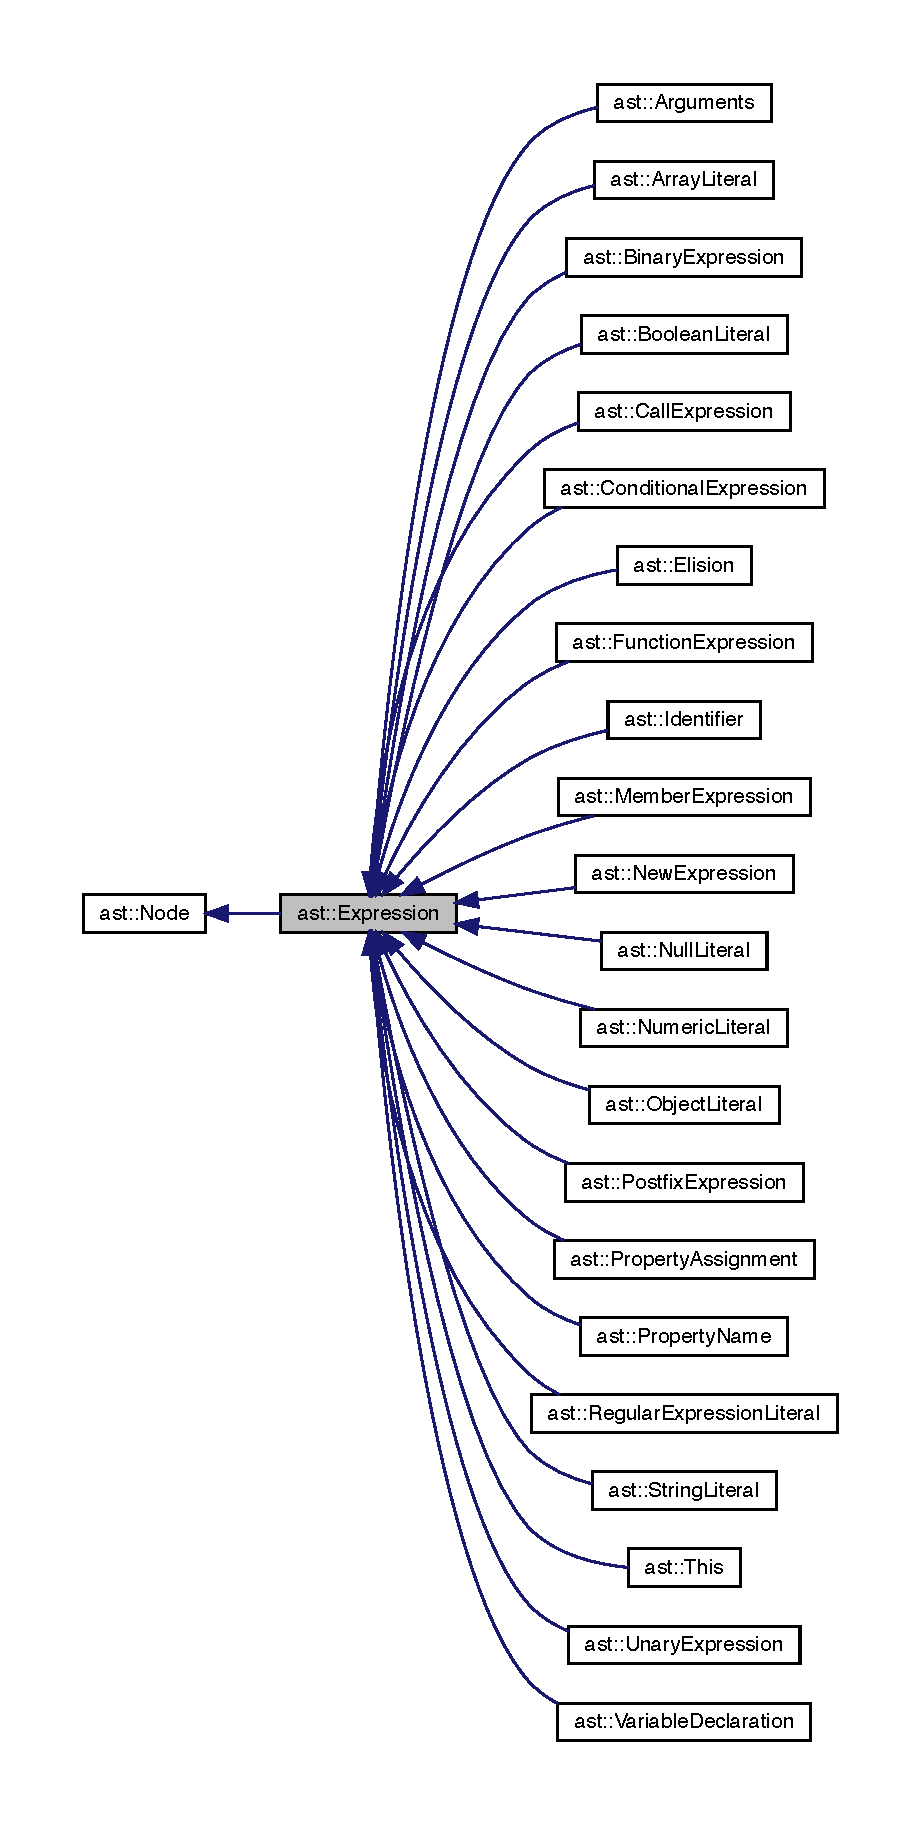
\includegraphics[width=350pt]{structast_1_1_expression__inherit__graph}
\end{center}
\end{figure}


Collaboration diagram for ast\+:\+:Expression\+:\nopagebreak
\begin{figure}[H]
\begin{center}
\leavevmode
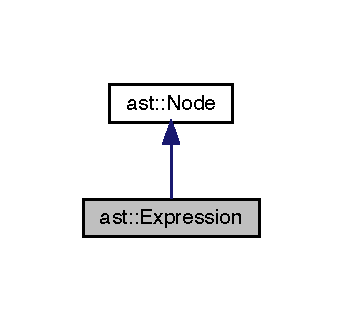
\includegraphics[width=164pt]{structast_1_1_expression__coll__graph}
\end{center}
\end{figure}
\subsection*{Additional Inherited Members}


The documentation for this struct was generated from the following file\+:\begin{DoxyCompactItemize}
\item 
src/\hyperlink{ast_8h}{ast.\+h}\end{DoxyCompactItemize}

\hypertarget{structast_1_1_expression_statement}{}\section{ast\+:\+:Expression\+Statement Struct Reference}
\label{structast_1_1_expression_statement}\index{ast\+::\+Expression\+Statement@{ast\+::\+Expression\+Statement}}


{\ttfamily \#include $<$ast.\+h$>$}



Inheritance diagram for ast\+:\+:Expression\+Statement\+:
\nopagebreak
\begin{figure}[H]
\begin{center}
\leavevmode
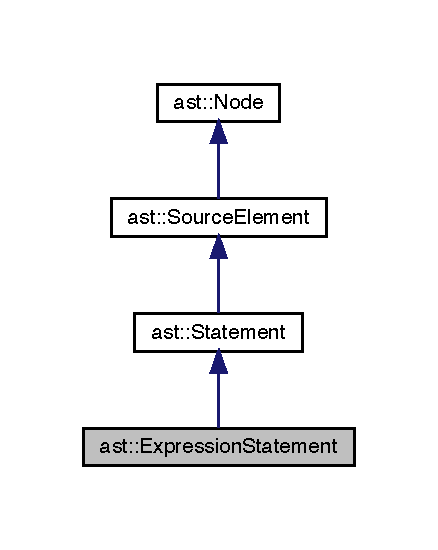
\includegraphics[width=210pt]{structast_1_1_expression_statement__inherit__graph}
\end{center}
\end{figure}


Collaboration diagram for ast\+:\+:Expression\+Statement\+:
\nopagebreak
\begin{figure}[H]
\begin{center}
\leavevmode
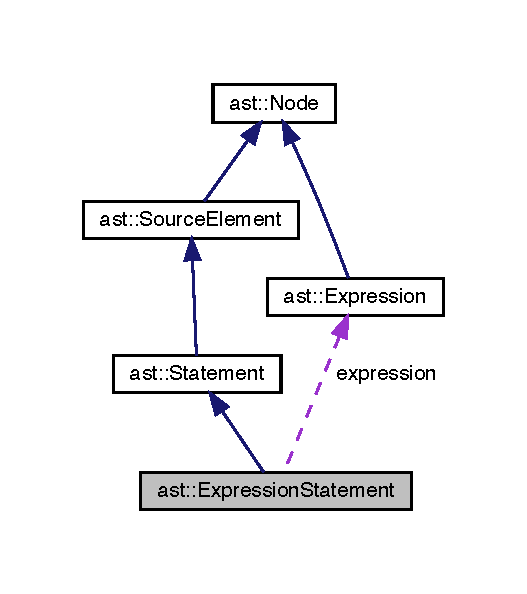
\includegraphics[width=253pt]{structast_1_1_expression_statement__coll__graph}
\end{center}
\end{figure}
\subsection*{Public Member Functions}
\begin{DoxyCompactItemize}
\item 
\hyperlink{structast_1_1_expression_statement_ae52db4b78ca0e4117e9b12b375d57260}{Expression\+Statement} (\hyperlink{structast_1_1_expression}{Expression} $\ast$\hyperlink{structast_1_1_expression_statement_a1829b79e8621555588c547173ae94c00}{expression})
\item 
void \hyperlink{structast_1_1_expression_statement_ae1423385af60671e488b20ecbbc1f86e}{accept} (\hyperlink{structast_1_1_visitor}{Visitor} \&visitor) const override
\end{DoxyCompactItemize}
\subsection*{Public Attributes}
\begin{DoxyCompactItemize}
\item 
\hyperlink{structast_1_1_expression}{Expression} $\ast$ \hyperlink{structast_1_1_expression_statement_a1829b79e8621555588c547173ae94c00}{expression}
\end{DoxyCompactItemize}


\subsection{Constructor \& Destructor Documentation}
\mbox{\Hypertarget{structast_1_1_expression_statement_ae52db4b78ca0e4117e9b12b375d57260}\label{structast_1_1_expression_statement_ae52db4b78ca0e4117e9b12b375d57260}} 
\index{ast\+::\+Expression\+Statement@{ast\+::\+Expression\+Statement}!Expression\+Statement@{Expression\+Statement}}
\index{Expression\+Statement@{Expression\+Statement}!ast\+::\+Expression\+Statement@{ast\+::\+Expression\+Statement}}
\subsubsection{\texorpdfstring{Expression\+Statement()}{ExpressionStatement()}}
{\footnotesize\ttfamily ast\+::\+Expression\+Statement\+::\+Expression\+Statement (\begin{DoxyParamCaption}\item[{\hyperlink{structast_1_1_expression}{Expression} $\ast$}]{expression }\end{DoxyParamCaption})\hspace{0.3cm}{\ttfamily [inline]}}



\subsection{Member Function Documentation}
\mbox{\Hypertarget{structast_1_1_expression_statement_ae1423385af60671e488b20ecbbc1f86e}\label{structast_1_1_expression_statement_ae1423385af60671e488b20ecbbc1f86e}} 
\index{ast\+::\+Expression\+Statement@{ast\+::\+Expression\+Statement}!accept@{accept}}
\index{accept@{accept}!ast\+::\+Expression\+Statement@{ast\+::\+Expression\+Statement}}
\subsubsection{\texorpdfstring{accept()}{accept()}}
{\footnotesize\ttfamily void ast\+::\+Expression\+Statement\+::accept (\begin{DoxyParamCaption}\item[{\hyperlink{structast_1_1_visitor}{Visitor} \&}]{visitor }\end{DoxyParamCaption}) const\hspace{0.3cm}{\ttfamily [inline]}, {\ttfamily [override]}, {\ttfamily [virtual]}}



Implements \hyperlink{structast_1_1_node_abc089ee6caaf06a4445ebdd8391fdebc}{ast\+::\+Node}.



\subsection{Member Data Documentation}
\mbox{\Hypertarget{structast_1_1_expression_statement_a1829b79e8621555588c547173ae94c00}\label{structast_1_1_expression_statement_a1829b79e8621555588c547173ae94c00}} 
\index{ast\+::\+Expression\+Statement@{ast\+::\+Expression\+Statement}!expression@{expression}}
\index{expression@{expression}!ast\+::\+Expression\+Statement@{ast\+::\+Expression\+Statement}}
\subsubsection{\texorpdfstring{expression}{expression}}
{\footnotesize\ttfamily \hyperlink{structast_1_1_expression}{Expression}$\ast$ ast\+::\+Expression\+Statement\+::expression}



The documentation for this struct was generated from the following file\+:\begin{DoxyCompactItemize}
\item 
src/\hyperlink{ast_8h}{ast.\+h}\end{DoxyCompactItemize}

\hypertarget{structast_1_1_for_in_statement}{}\section{ast\+:\+:For\+In\+Statement Struct Reference}
\label{structast_1_1_for_in_statement}\index{ast\+::\+For\+In\+Statement@{ast\+::\+For\+In\+Statement}}


{\ttfamily \#include $<$ast.\+h$>$}



Inheritance diagram for ast\+:\+:For\+In\+Statement\+:
\nopagebreak
\begin{figure}[H]
\begin{center}
\leavevmode
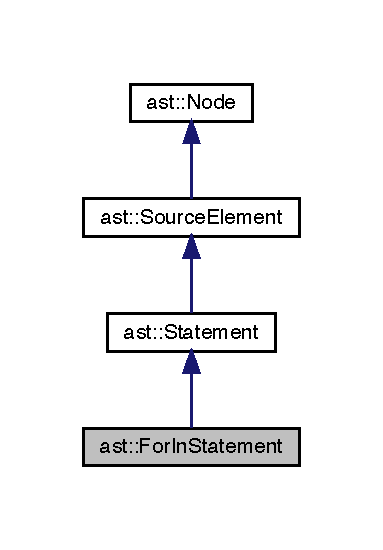
\includegraphics[width=184pt]{structast_1_1_for_in_statement__inherit__graph}
\end{center}
\end{figure}


Collaboration diagram for ast\+:\+:For\+In\+Statement\+:
\nopagebreak
\begin{figure}[H]
\begin{center}
\leavevmode
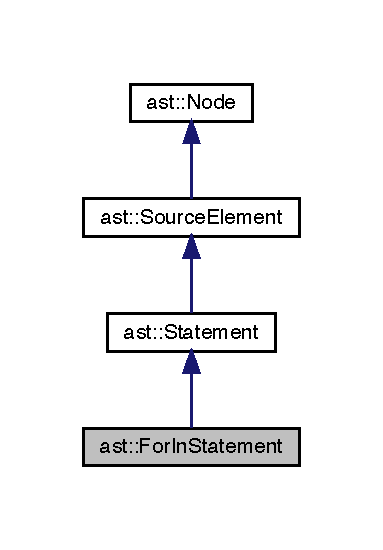
\includegraphics[width=184pt]{structast_1_1_for_in_statement__coll__graph}
\end{center}
\end{figure}
\subsection*{Public Member Functions}
\begin{DoxyCompactItemize}
\item 
void \hyperlink{structast_1_1_for_in_statement_a9322c609ad608ac86f4afb4170d6ffff}{accept} (\hyperlink{structast_1_1_visitor}{Visitor} \&visitor) const override
\end{DoxyCompactItemize}


\subsection{Member Function Documentation}
\mbox{\Hypertarget{structast_1_1_for_in_statement_a9322c609ad608ac86f4afb4170d6ffff}\label{structast_1_1_for_in_statement_a9322c609ad608ac86f4afb4170d6ffff}} 
\index{ast\+::\+For\+In\+Statement@{ast\+::\+For\+In\+Statement}!accept@{accept}}
\index{accept@{accept}!ast\+::\+For\+In\+Statement@{ast\+::\+For\+In\+Statement}}
\subsubsection{\texorpdfstring{accept()}{accept()}}
{\footnotesize\ttfamily void ast\+::\+For\+In\+Statement\+::accept (\begin{DoxyParamCaption}\item[{\hyperlink{structast_1_1_visitor}{Visitor} \&}]{visitor }\end{DoxyParamCaption}) const\hspace{0.3cm}{\ttfamily [inline]}, {\ttfamily [override]}, {\ttfamily [virtual]}}



Implements \hyperlink{structast_1_1_node_abc089ee6caaf06a4445ebdd8391fdebc}{ast\+::\+Node}.



The documentation for this struct was generated from the following file\+:\begin{DoxyCompactItemize}
\item 
src/\hyperlink{ast_8h}{ast.\+h}\end{DoxyCompactItemize}

\hypertarget{structast_1_1_formal_parameter_list}{}\section{ast\+:\+:Formal\+Parameter\+List Struct Reference}
\label{structast_1_1_formal_parameter_list}\index{ast\+::\+Formal\+Parameter\+List@{ast\+::\+Formal\+Parameter\+List}}


{\ttfamily \#include $<$ast.\+h$>$}



Inheritance diagram for ast\+:\+:Formal\+Parameter\+List\+:\nopagebreak
\begin{figure}[H]
\begin{center}
\leavevmode
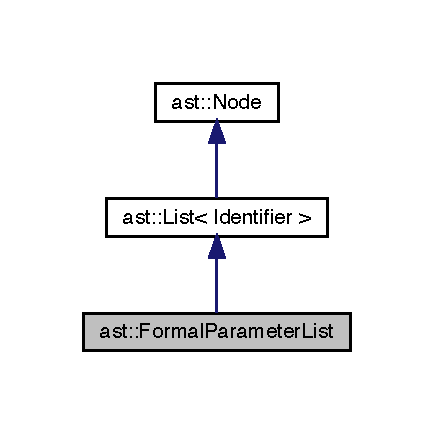
\includegraphics[width=208pt]{structast_1_1_formal_parameter_list__inherit__graph}
\end{center}
\end{figure}


Collaboration diagram for ast\+:\+:Formal\+Parameter\+List\+:\nopagebreak
\begin{figure}[H]
\begin{center}
\leavevmode
\includegraphics[width=278pt]{structast_1_1_formal_parameter_list__coll__graph}
\end{center}
\end{figure}
\subsection*{Additional Inherited Members}


The documentation for this struct was generated from the following file\+:\begin{DoxyCompactItemize}
\item 
src/\hyperlink{ast_8h}{ast.\+h}\end{DoxyCompactItemize}

\hypertarget{structast_1_1_for_statement}{}\section{ast\+:\+:For\+Statement Struct Reference}
\label{structast_1_1_for_statement}\index{ast\+::\+For\+Statement@{ast\+::\+For\+Statement}}


{\ttfamily \#include $<$ast.\+h$>$}



Inheritance diagram for ast\+:\+:For\+Statement\+:
\nopagebreak
\begin{figure}[H]
\begin{center}
\leavevmode
\includegraphics[width=183pt]{structast_1_1_for_statement__inherit__graph}
\end{center}
\end{figure}


Collaboration diagram for ast\+:\+:For\+Statement\+:
\nopagebreak
\begin{figure}[H]
\begin{center}
\leavevmode
\includegraphics[width=183pt]{structast_1_1_for_statement__coll__graph}
\end{center}
\end{figure}
\subsection*{Public Member Functions}
\begin{DoxyCompactItemize}
\item 
void \hyperlink{structast_1_1_for_statement_af2a457b14c605b01216ec6f950e36e94}{accept} (\hyperlink{structast_1_1_visitor}{Visitor} \&visitor) const override
\end{DoxyCompactItemize}


\subsection{Member Function Documentation}
\mbox{\Hypertarget{structast_1_1_for_statement_af2a457b14c605b01216ec6f950e36e94}\label{structast_1_1_for_statement_af2a457b14c605b01216ec6f950e36e94}} 
\index{ast\+::\+For\+Statement@{ast\+::\+For\+Statement}!accept@{accept}}
\index{accept@{accept}!ast\+::\+For\+Statement@{ast\+::\+For\+Statement}}
\subsubsection{\texorpdfstring{accept()}{accept()}}
{\footnotesize\ttfamily void ast\+::\+For\+Statement\+::accept (\begin{DoxyParamCaption}\item[{\hyperlink{structast_1_1_visitor}{Visitor} \&}]{visitor }\end{DoxyParamCaption}) const\hspace{0.3cm}{\ttfamily [inline]}, {\ttfamily [override]}, {\ttfamily [virtual]}}



Implements \hyperlink{structast_1_1_node_abc089ee6caaf06a4445ebdd8391fdebc}{ast\+::\+Node}.



The documentation for this struct was generated from the following file\+:\begin{DoxyCompactItemize}
\item 
src/\hyperlink{ast_8h}{ast.\+h}\end{DoxyCompactItemize}

\hypertarget{structast_1_1_function_body}{}\section{ast\+:\+:Function\+Body Struct Reference}
\label{structast_1_1_function_body}\index{ast\+::\+Function\+Body@{ast\+::\+Function\+Body}}


{\ttfamily \#include $<$ast.\+h$>$}



Inheritance diagram for ast\+:\+:Function\+Body\+:
\nopagebreak
\begin{figure}[H]
\begin{center}
\leavevmode
\includegraphics[width=216pt]{structast_1_1_function_body__inherit__graph}
\end{center}
\end{figure}


Collaboration diagram for ast\+:\+:Function\+Body\+:
\nopagebreak
\begin{figure}[H]
\begin{center}
\leavevmode
\includegraphics[width=308pt]{structast_1_1_function_body__coll__graph}
\end{center}
\end{figure}
\subsection*{Public Member Functions}
\begin{DoxyCompactItemize}
\item 
\hyperlink{structast_1_1_function_body_af0d6be1290af04c42862db2d5831ab0b}{Function\+Body} (\hyperlink{structast_1_1_source_elements}{Source\+Elements} $\ast$body=nullptr)
\item 
void \hyperlink{structast_1_1_function_body_a499e419e1516c0dd36b2edd325fd23b4}{accept} (\hyperlink{structast_1_1_visitor}{Visitor} \&visitor) const override
\end{DoxyCompactItemize}
\subsection*{Additional Inherited Members}


\subsection{Constructor \& Destructor Documentation}
\mbox{\Hypertarget{structast_1_1_function_body_af0d6be1290af04c42862db2d5831ab0b}\label{structast_1_1_function_body_af0d6be1290af04c42862db2d5831ab0b}} 
\index{ast\+::\+Function\+Body@{ast\+::\+Function\+Body}!Function\+Body@{Function\+Body}}
\index{Function\+Body@{Function\+Body}!ast\+::\+Function\+Body@{ast\+::\+Function\+Body}}
\subsubsection{\texorpdfstring{Function\+Body()}{FunctionBody()}}
{\footnotesize\ttfamily ast\+::\+Function\+Body\+::\+Function\+Body (\begin{DoxyParamCaption}\item[{\hyperlink{structast_1_1_source_elements}{Source\+Elements} $\ast$}]{body = {\ttfamily nullptr} }\end{DoxyParamCaption})\hspace{0.3cm}{\ttfamily [inline]}}



\subsection{Member Function Documentation}
\mbox{\Hypertarget{structast_1_1_function_body_a499e419e1516c0dd36b2edd325fd23b4}\label{structast_1_1_function_body_a499e419e1516c0dd36b2edd325fd23b4}} 
\index{ast\+::\+Function\+Body@{ast\+::\+Function\+Body}!accept@{accept}}
\index{accept@{accept}!ast\+::\+Function\+Body@{ast\+::\+Function\+Body}}
\subsubsection{\texorpdfstring{accept()}{accept()}}
{\footnotesize\ttfamily void ast\+::\+Function\+Body\+::accept (\begin{DoxyParamCaption}\item[{\hyperlink{structast_1_1_visitor}{Visitor} \&}]{visitor }\end{DoxyParamCaption}) const\hspace{0.3cm}{\ttfamily [inline]}, {\ttfamily [override]}, {\ttfamily [virtual]}}



Implements \hyperlink{structast_1_1_node_abc089ee6caaf06a4445ebdd8391fdebc}{ast\+::\+Node}.



The documentation for this struct was generated from the following file\+:\begin{DoxyCompactItemize}
\item 
src/\hyperlink{ast_8h}{ast.\+h}\end{DoxyCompactItemize}

\hypertarget{structast_1_1_function_declaration}{}\section{ast\+:\+:Function\+Declaration Struct Reference}
\label{structast_1_1_function_declaration}\index{ast\+::\+Function\+Declaration@{ast\+::\+Function\+Declaration}}


{\ttfamily \#include $<$ast.\+h$>$}



Inheritance diagram for ast\+:\+:Function\+Declaration\+:
\nopagebreak
\begin{figure}[H]
\begin{center}
\leavevmode
\includegraphics[width=204pt]{structast_1_1_function_declaration__inherit__graph}
\end{center}
\end{figure}


Collaboration diagram for ast\+:\+:Function\+Declaration\+:
\nopagebreak
\begin{figure}[H]
\begin{center}
\leavevmode
\includegraphics[width=350pt]{structast_1_1_function_declaration__coll__graph}
\end{center}
\end{figure}
\subsection*{Public Member Functions}
\begin{DoxyCompactItemize}
\item 
\hyperlink{structast_1_1_function_declaration_afd97d059c7498c536e486adb81b4c269}{Function\+Declaration} (\hyperlink{structast_1_1_identifier}{Identifier} $\ast$\hyperlink{structast_1_1_function_declaration_aa593ce68ef88fb6cf977062b1af99ccd}{id}, \hyperlink{structast_1_1_formal_parameter_list}{Formal\+Parameter\+List} $\ast$\hyperlink{structast_1_1_function_declaration_aff742e988b196183febb9b3acbe04739}{params}, \hyperlink{structast_1_1_function_body}{Function\+Body} $\ast$\hyperlink{structast_1_1_function_declaration_a35686e34a8dc7de03745a0e8890b7bf4}{body})
\item 
void \hyperlink{structast_1_1_function_declaration_a870a888ed05b4fbe6e724652ae2c6442}{accept} (\hyperlink{structast_1_1_visitor}{Visitor} \&visitor) const
\end{DoxyCompactItemize}
\subsection*{Public Attributes}
\begin{DoxyCompactItemize}
\item 
\hyperlink{structast_1_1_identifier}{Identifier} $\ast$ \hyperlink{structast_1_1_function_declaration_aa593ce68ef88fb6cf977062b1af99ccd}{id}
\item 
\hyperlink{structast_1_1_formal_parameter_list}{Formal\+Parameter\+List} $\ast$ \hyperlink{structast_1_1_function_declaration_aff742e988b196183febb9b3acbe04739}{params}
\item 
\hyperlink{structast_1_1_function_body}{Function\+Body} $\ast$ \hyperlink{structast_1_1_function_declaration_a35686e34a8dc7de03745a0e8890b7bf4}{body}
\end{DoxyCompactItemize}


\subsection{Constructor \& Destructor Documentation}
\mbox{\Hypertarget{structast_1_1_function_declaration_afd97d059c7498c536e486adb81b4c269}\label{structast_1_1_function_declaration_afd97d059c7498c536e486adb81b4c269}} 
\index{ast\+::\+Function\+Declaration@{ast\+::\+Function\+Declaration}!Function\+Declaration@{Function\+Declaration}}
\index{Function\+Declaration@{Function\+Declaration}!ast\+::\+Function\+Declaration@{ast\+::\+Function\+Declaration}}
\subsubsection{\texorpdfstring{Function\+Declaration()}{FunctionDeclaration()}}
{\footnotesize\ttfamily ast\+::\+Function\+Declaration\+::\+Function\+Declaration (\begin{DoxyParamCaption}\item[{\hyperlink{structast_1_1_identifier}{Identifier} $\ast$}]{id,  }\item[{\hyperlink{structast_1_1_formal_parameter_list}{Formal\+Parameter\+List} $\ast$}]{params,  }\item[{\hyperlink{structast_1_1_function_body}{Function\+Body} $\ast$}]{body }\end{DoxyParamCaption})\hspace{0.3cm}{\ttfamily [inline]}}



\subsection{Member Function Documentation}
\mbox{\Hypertarget{structast_1_1_function_declaration_a870a888ed05b4fbe6e724652ae2c6442}\label{structast_1_1_function_declaration_a870a888ed05b4fbe6e724652ae2c6442}} 
\index{ast\+::\+Function\+Declaration@{ast\+::\+Function\+Declaration}!accept@{accept}}
\index{accept@{accept}!ast\+::\+Function\+Declaration@{ast\+::\+Function\+Declaration}}
\subsubsection{\texorpdfstring{accept()}{accept()}}
{\footnotesize\ttfamily void ast\+::\+Function\+Declaration\+::accept (\begin{DoxyParamCaption}\item[{\hyperlink{structast_1_1_visitor}{Visitor} \&}]{visitor }\end{DoxyParamCaption}) const\hspace{0.3cm}{\ttfamily [inline]}, {\ttfamily [virtual]}}



Implements \hyperlink{structast_1_1_node_abc089ee6caaf06a4445ebdd8391fdebc}{ast\+::\+Node}.



\subsection{Member Data Documentation}
\mbox{\Hypertarget{structast_1_1_function_declaration_a35686e34a8dc7de03745a0e8890b7bf4}\label{structast_1_1_function_declaration_a35686e34a8dc7de03745a0e8890b7bf4}} 
\index{ast\+::\+Function\+Declaration@{ast\+::\+Function\+Declaration}!body@{body}}
\index{body@{body}!ast\+::\+Function\+Declaration@{ast\+::\+Function\+Declaration}}
\subsubsection{\texorpdfstring{body}{body}}
{\footnotesize\ttfamily \hyperlink{structast_1_1_function_body}{Function\+Body}$\ast$ ast\+::\+Function\+Declaration\+::body}

\mbox{\Hypertarget{structast_1_1_function_declaration_aa593ce68ef88fb6cf977062b1af99ccd}\label{structast_1_1_function_declaration_aa593ce68ef88fb6cf977062b1af99ccd}} 
\index{ast\+::\+Function\+Declaration@{ast\+::\+Function\+Declaration}!id@{id}}
\index{id@{id}!ast\+::\+Function\+Declaration@{ast\+::\+Function\+Declaration}}
\subsubsection{\texorpdfstring{id}{id}}
{\footnotesize\ttfamily \hyperlink{structast_1_1_identifier}{Identifier}$\ast$ ast\+::\+Function\+Declaration\+::id}

\mbox{\Hypertarget{structast_1_1_function_declaration_aff742e988b196183febb9b3acbe04739}\label{structast_1_1_function_declaration_aff742e988b196183febb9b3acbe04739}} 
\index{ast\+::\+Function\+Declaration@{ast\+::\+Function\+Declaration}!params@{params}}
\index{params@{params}!ast\+::\+Function\+Declaration@{ast\+::\+Function\+Declaration}}
\subsubsection{\texorpdfstring{params}{params}}
{\footnotesize\ttfamily \hyperlink{structast_1_1_formal_parameter_list}{Formal\+Parameter\+List}$\ast$ ast\+::\+Function\+Declaration\+::params}



The documentation for this struct was generated from the following file\+:\begin{DoxyCompactItemize}
\item 
src/\hyperlink{ast_8h}{ast.\+h}\end{DoxyCompactItemize}

\hypertarget{structast_1_1_function_expression}{}\section{ast\+:\+:Function\+Expression Struct Reference}
\label{structast_1_1_function_expression}\index{ast\+::\+Function\+Expression@{ast\+::\+Function\+Expression}}


{\ttfamily \#include $<$ast.\+h$>$}



Inheritance diagram for ast\+:\+:Function\+Expression\+:\nopagebreak
\begin{figure}[H]
\begin{center}
\leavevmode
\includegraphics[width=203pt]{structast_1_1_function_expression__inherit__graph}
\end{center}
\end{figure}


Collaboration diagram for ast\+:\+:Function\+Expression\+:\nopagebreak
\begin{figure}[H]
\begin{center}
\leavevmode
\includegraphics[width=350pt]{structast_1_1_function_expression__coll__graph}
\end{center}
\end{figure}
\subsection*{Public Member Functions}
\begin{DoxyCompactItemize}
\item 
\hyperlink{structast_1_1_function_expression_a378f9e09b02d457e88b4b71e169e2154}{Function\+Expression} (\hyperlink{structast_1_1_identifier}{Identifier} $\ast$\hyperlink{structast_1_1_function_expression_af3439c30bbde4463bc71158f24b1dd13}{id}, \hyperlink{structast_1_1_formal_parameter_list}{Formal\+Parameter\+List} $\ast$\hyperlink{structast_1_1_function_expression_a83a7dd9fe27f5e9f6357f398d52476e3}{params}, \hyperlink{structast_1_1_function_body}{Function\+Body} $\ast$\hyperlink{structast_1_1_function_expression_a708305d4b4f5421d1dfcbe5edb15374c}{body})
\item 
void \hyperlink{structast_1_1_function_expression_aa847bb46bcd639d92e0fd2bc0bcf0a3f}{accept} (\hyperlink{structast_1_1_visitor}{Visitor} \&visitor) const
\end{DoxyCompactItemize}
\subsection*{Public Attributes}
\begin{DoxyCompactItemize}
\item 
\hyperlink{structast_1_1_identifier}{Identifier} $\ast$ \hyperlink{structast_1_1_function_expression_af3439c30bbde4463bc71158f24b1dd13}{id}
\item 
\hyperlink{structast_1_1_formal_parameter_list}{Formal\+Parameter\+List} $\ast$ \hyperlink{structast_1_1_function_expression_a83a7dd9fe27f5e9f6357f398d52476e3}{params}
\item 
\hyperlink{structast_1_1_function_body}{Function\+Body} $\ast$ \hyperlink{structast_1_1_function_expression_a708305d4b4f5421d1dfcbe5edb15374c}{body}
\end{DoxyCompactItemize}


\subsection{Constructor \& Destructor Documentation}
\mbox{\Hypertarget{structast_1_1_function_expression_a378f9e09b02d457e88b4b71e169e2154}\label{structast_1_1_function_expression_a378f9e09b02d457e88b4b71e169e2154}} 
\index{ast\+::\+Function\+Expression@{ast\+::\+Function\+Expression}!Function\+Expression@{Function\+Expression}}
\index{Function\+Expression@{Function\+Expression}!ast\+::\+Function\+Expression@{ast\+::\+Function\+Expression}}
\subsubsection{\texorpdfstring{Function\+Expression()}{FunctionExpression()}}
{\footnotesize\ttfamily ast\+::\+Function\+Expression\+::\+Function\+Expression (\begin{DoxyParamCaption}\item[{\hyperlink{structast_1_1_identifier}{Identifier} $\ast$}]{id,  }\item[{\hyperlink{structast_1_1_formal_parameter_list}{Formal\+Parameter\+List} $\ast$}]{params,  }\item[{\hyperlink{structast_1_1_function_body}{Function\+Body} $\ast$}]{body }\end{DoxyParamCaption})\hspace{0.3cm}{\ttfamily [inline]}}



\subsection{Member Function Documentation}
\mbox{\Hypertarget{structast_1_1_function_expression_aa847bb46bcd639d92e0fd2bc0bcf0a3f}\label{structast_1_1_function_expression_aa847bb46bcd639d92e0fd2bc0bcf0a3f}} 
\index{ast\+::\+Function\+Expression@{ast\+::\+Function\+Expression}!accept@{accept}}
\index{accept@{accept}!ast\+::\+Function\+Expression@{ast\+::\+Function\+Expression}}
\subsubsection{\texorpdfstring{accept()}{accept()}}
{\footnotesize\ttfamily void ast\+::\+Function\+Expression\+::accept (\begin{DoxyParamCaption}\item[{\hyperlink{structast_1_1_visitor}{Visitor} \&}]{visitor }\end{DoxyParamCaption}) const\hspace{0.3cm}{\ttfamily [inline]}, {\ttfamily [virtual]}}



Implements \hyperlink{structast_1_1_node_abc089ee6caaf06a4445ebdd8391fdebc}{ast\+::\+Node}.



\subsection{Member Data Documentation}
\mbox{\Hypertarget{structast_1_1_function_expression_a708305d4b4f5421d1dfcbe5edb15374c}\label{structast_1_1_function_expression_a708305d4b4f5421d1dfcbe5edb15374c}} 
\index{ast\+::\+Function\+Expression@{ast\+::\+Function\+Expression}!body@{body}}
\index{body@{body}!ast\+::\+Function\+Expression@{ast\+::\+Function\+Expression}}
\subsubsection{\texorpdfstring{body}{body}}
{\footnotesize\ttfamily \hyperlink{structast_1_1_function_body}{Function\+Body}$\ast$ ast\+::\+Function\+Expression\+::body}

\mbox{\Hypertarget{structast_1_1_function_expression_af3439c30bbde4463bc71158f24b1dd13}\label{structast_1_1_function_expression_af3439c30bbde4463bc71158f24b1dd13}} 
\index{ast\+::\+Function\+Expression@{ast\+::\+Function\+Expression}!id@{id}}
\index{id@{id}!ast\+::\+Function\+Expression@{ast\+::\+Function\+Expression}}
\subsubsection{\texorpdfstring{id}{id}}
{\footnotesize\ttfamily \hyperlink{structast_1_1_identifier}{Identifier}$\ast$ ast\+::\+Function\+Expression\+::id}

\mbox{\Hypertarget{structast_1_1_function_expression_a83a7dd9fe27f5e9f6357f398d52476e3}\label{structast_1_1_function_expression_a83a7dd9fe27f5e9f6357f398d52476e3}} 
\index{ast\+::\+Function\+Expression@{ast\+::\+Function\+Expression}!params@{params}}
\index{params@{params}!ast\+::\+Function\+Expression@{ast\+::\+Function\+Expression}}
\subsubsection{\texorpdfstring{params}{params}}
{\footnotesize\ttfamily \hyperlink{structast_1_1_formal_parameter_list}{Formal\+Parameter\+List}$\ast$ ast\+::\+Function\+Expression\+::params}



The documentation for this struct was generated from the following file\+:\begin{DoxyCompactItemize}
\item 
src/\hyperlink{ast_8h}{ast.\+h}\end{DoxyCompactItemize}

\hypertarget{structast_1_1_identifier}{}\section{ast\+:\+:Identifier Struct Reference}
\label{structast_1_1_identifier}\index{ast\+::\+Identifier@{ast\+::\+Identifier}}


{\ttfamily \#include $<$ast.\+h$>$}



Inheritance diagram for ast\+:\+:Identifier\+:
\nopagebreak
\begin{figure}[H]
\begin{center}
\leavevmode
\includegraphics[width=199pt]{structast_1_1_identifier__inherit__graph}
\end{center}
\end{figure}


Collaboration diagram for ast\+:\+:Identifier\+:
\nopagebreak
\begin{figure}[H]
\begin{center}
\leavevmode
\includegraphics[width=292pt]{structast_1_1_identifier__coll__graph}
\end{center}
\end{figure}
\subsection*{Public Member Functions}
\begin{DoxyCompactItemize}
\item 
\hyperlink{structast_1_1_identifier_ad1c565306c43b4b5fcacee989b9bab6f}{Identifier} (\textbf{ std\+::u16string} \hyperlink{structast_1_1_identifier_a94073f3af4a0e4accf4dfd4efb8e572e}{value})
\item 
void \hyperlink{structast_1_1_identifier_a4be0b28397f057ed7ec88234bb23bded}{accept} (\hyperlink{structast_1_1_visitor}{Visitor} \&visitor) const override
\end{DoxyCompactItemize}
\subsection*{Public Attributes}
\begin{DoxyCompactItemize}
\item 
\textbf{ std\+::u16string} \hyperlink{structast_1_1_identifier_a94073f3af4a0e4accf4dfd4efb8e572e}{value}
\end{DoxyCompactItemize}


\subsection{Constructor \& Destructor Documentation}
\mbox{\Hypertarget{structast_1_1_identifier_ad1c565306c43b4b5fcacee989b9bab6f}\label{structast_1_1_identifier_ad1c565306c43b4b5fcacee989b9bab6f}} 
\index{ast\+::\+Identifier@{ast\+::\+Identifier}!Identifier@{Identifier}}
\index{Identifier@{Identifier}!ast\+::\+Identifier@{ast\+::\+Identifier}}
\subsubsection{\texorpdfstring{Identifier()}{Identifier()}}
{\footnotesize\ttfamily ast\+::\+Identifier\+::\+Identifier (\begin{DoxyParamCaption}\item[{\textbf{ std\+::u16string}}]{value }\end{DoxyParamCaption})\hspace{0.3cm}{\ttfamily [inline]}}



\subsection{Member Function Documentation}
\mbox{\Hypertarget{structast_1_1_identifier_a4be0b28397f057ed7ec88234bb23bded}\label{structast_1_1_identifier_a4be0b28397f057ed7ec88234bb23bded}} 
\index{ast\+::\+Identifier@{ast\+::\+Identifier}!accept@{accept}}
\index{accept@{accept}!ast\+::\+Identifier@{ast\+::\+Identifier}}
\subsubsection{\texorpdfstring{accept()}{accept()}}
{\footnotesize\ttfamily void ast\+::\+Identifier\+::accept (\begin{DoxyParamCaption}\item[{\hyperlink{structast_1_1_visitor}{Visitor} \&}]{visitor }\end{DoxyParamCaption}) const\hspace{0.3cm}{\ttfamily [inline]}, {\ttfamily [override]}, {\ttfamily [virtual]}}



Implements \hyperlink{structast_1_1_node_abc089ee6caaf06a4445ebdd8391fdebc}{ast\+::\+Node}.



\subsection{Member Data Documentation}
\mbox{\Hypertarget{structast_1_1_identifier_a94073f3af4a0e4accf4dfd4efb8e572e}\label{structast_1_1_identifier_a94073f3af4a0e4accf4dfd4efb8e572e}} 
\index{ast\+::\+Identifier@{ast\+::\+Identifier}!value@{value}}
\index{value@{value}!ast\+::\+Identifier@{ast\+::\+Identifier}}
\subsubsection{\texorpdfstring{value}{value}}
{\footnotesize\ttfamily \textbf{ std\+::u16string} ast\+::\+Identifier\+::value}



The documentation for this struct was generated from the following file\+:\begin{DoxyCompactItemize}
\item 
src/\hyperlink{ast_8h}{ast.\+h}\end{DoxyCompactItemize}

\hypertarget{structast_1_1_if_statement}{}\section{ast\+:\+:If\+Statement Struct Reference}
\label{structast_1_1_if_statement}\index{ast\+::\+If\+Statement@{ast\+::\+If\+Statement}}


{\ttfamily \#include $<$ast.\+h$>$}



Inheritance diagram for ast\+:\+:If\+Statement\+:\nopagebreak
\begin{figure}[H]
\begin{center}
\leavevmode
\includegraphics[width=183pt]{structast_1_1_if_statement__inherit__graph}
\end{center}
\end{figure}


Collaboration diagram for ast\+:\+:If\+Statement\+:\nopagebreak
\begin{figure}[H]
\begin{center}
\leavevmode
\includegraphics[width=254pt]{structast_1_1_if_statement__coll__graph}
\end{center}
\end{figure}
\subsection*{Public Member Functions}
\begin{DoxyCompactItemize}
\item 
\hyperlink{structast_1_1_if_statement_adab903b8789a25744b1607ded9dca1d2}{If\+Statement} (\hyperlink{structast_1_1_expression}{Expression} $\ast$\hyperlink{structast_1_1_if_statement_ad339145ed98fc65452bc7339f737a790}{test}, \hyperlink{structast_1_1_statement}{Statement} $\ast$\hyperlink{structast_1_1_if_statement_a2a02f92cb28fb4847ea286341c1c0270}{consequent}, \hyperlink{structast_1_1_statement}{Statement} $\ast$\hyperlink{structast_1_1_if_statement_a2f84078dbbe4d3246609c13c526fc69d}{alternate}=nullptr)
\item 
void \hyperlink{structast_1_1_if_statement_ab4053b9564cf00687f8f1351dd8044cb}{accept} (\hyperlink{structast_1_1_visitor}{Visitor} \&visitor) const override
\end{DoxyCompactItemize}
\subsection*{Public Attributes}
\begin{DoxyCompactItemize}
\item 
\hyperlink{structast_1_1_expression}{Expression} $\ast$ \hyperlink{structast_1_1_if_statement_ad339145ed98fc65452bc7339f737a790}{test}
\item 
\hyperlink{structast_1_1_statement}{Statement} $\ast$ \hyperlink{structast_1_1_if_statement_a2a02f92cb28fb4847ea286341c1c0270}{consequent}
\item 
\hyperlink{structast_1_1_statement}{Statement} $\ast$ \hyperlink{structast_1_1_if_statement_a2f84078dbbe4d3246609c13c526fc69d}{alternate}
\end{DoxyCompactItemize}


\subsection{Constructor \& Destructor Documentation}
\mbox{\Hypertarget{structast_1_1_if_statement_adab903b8789a25744b1607ded9dca1d2}\label{structast_1_1_if_statement_adab903b8789a25744b1607ded9dca1d2}} 
\index{ast\+::\+If\+Statement@{ast\+::\+If\+Statement}!If\+Statement@{If\+Statement}}
\index{If\+Statement@{If\+Statement}!ast\+::\+If\+Statement@{ast\+::\+If\+Statement}}
\subsubsection{\texorpdfstring{If\+Statement()}{IfStatement()}}
{\footnotesize\ttfamily ast\+::\+If\+Statement\+::\+If\+Statement (\begin{DoxyParamCaption}\item[{\hyperlink{structast_1_1_expression}{Expression} $\ast$}]{test,  }\item[{\hyperlink{structast_1_1_statement}{Statement} $\ast$}]{consequent,  }\item[{\hyperlink{structast_1_1_statement}{Statement} $\ast$}]{alternate = {\ttfamily nullptr} }\end{DoxyParamCaption})\hspace{0.3cm}{\ttfamily [inline]}}



\subsection{Member Function Documentation}
\mbox{\Hypertarget{structast_1_1_if_statement_ab4053b9564cf00687f8f1351dd8044cb}\label{structast_1_1_if_statement_ab4053b9564cf00687f8f1351dd8044cb}} 
\index{ast\+::\+If\+Statement@{ast\+::\+If\+Statement}!accept@{accept}}
\index{accept@{accept}!ast\+::\+If\+Statement@{ast\+::\+If\+Statement}}
\subsubsection{\texorpdfstring{accept()}{accept()}}
{\footnotesize\ttfamily void ast\+::\+If\+Statement\+::accept (\begin{DoxyParamCaption}\item[{\hyperlink{structast_1_1_visitor}{Visitor} \&}]{visitor }\end{DoxyParamCaption}) const\hspace{0.3cm}{\ttfamily [inline]}, {\ttfamily [override]}, {\ttfamily [virtual]}}



Implements \hyperlink{structast_1_1_node_abc089ee6caaf06a4445ebdd8391fdebc}{ast\+::\+Node}.



\subsection{Member Data Documentation}
\mbox{\Hypertarget{structast_1_1_if_statement_a2f84078dbbe4d3246609c13c526fc69d}\label{structast_1_1_if_statement_a2f84078dbbe4d3246609c13c526fc69d}} 
\index{ast\+::\+If\+Statement@{ast\+::\+If\+Statement}!alternate@{alternate}}
\index{alternate@{alternate}!ast\+::\+If\+Statement@{ast\+::\+If\+Statement}}
\subsubsection{\texorpdfstring{alternate}{alternate}}
{\footnotesize\ttfamily \hyperlink{structast_1_1_statement}{Statement}$\ast$ ast\+::\+If\+Statement\+::alternate}

\mbox{\Hypertarget{structast_1_1_if_statement_a2a02f92cb28fb4847ea286341c1c0270}\label{structast_1_1_if_statement_a2a02f92cb28fb4847ea286341c1c0270}} 
\index{ast\+::\+If\+Statement@{ast\+::\+If\+Statement}!consequent@{consequent}}
\index{consequent@{consequent}!ast\+::\+If\+Statement@{ast\+::\+If\+Statement}}
\subsubsection{\texorpdfstring{consequent}{consequent}}
{\footnotesize\ttfamily \hyperlink{structast_1_1_statement}{Statement}$\ast$ ast\+::\+If\+Statement\+::consequent}

\mbox{\Hypertarget{structast_1_1_if_statement_ad339145ed98fc65452bc7339f737a790}\label{structast_1_1_if_statement_ad339145ed98fc65452bc7339f737a790}} 
\index{ast\+::\+If\+Statement@{ast\+::\+If\+Statement}!test@{test}}
\index{test@{test}!ast\+::\+If\+Statement@{ast\+::\+If\+Statement}}
\subsubsection{\texorpdfstring{test}{test}}
{\footnotesize\ttfamily \hyperlink{structast_1_1_expression}{Expression}$\ast$ ast\+::\+If\+Statement\+::test}



The documentation for this struct was generated from the following file\+:\begin{DoxyCompactItemize}
\item 
src/\hyperlink{ast_8h}{ast.\+h}\end{DoxyCompactItemize}

\hypertarget{class_input_element}{}\section{Input\+Element Class Reference}
\label{class_input_element}\index{Input\+Element@{Input\+Element}}


{\ttfamily \#include $<$input\+\_\+element.\+h$>$}

\subsection*{Public Member Functions}
\begin{DoxyCompactItemize}
\item 
bool \hyperlink{class_input_element_a4e4b6b2005fe0b8d07f30ef27210a51b}{is\+\_\+empty} () const
\item 
bool \hyperlink{class_input_element_a6bac1905f5d9aa43f89e1bbfdb553c15}{is\+\_\+token} () const
\item 
bool \hyperlink{class_input_element_adef5e449a8107adaac4f570994d698b9}{is\+\_\+line\+\_\+terminator} () const
\item 
bool \hyperlink{class_input_element_a1e2afc5eda150e298c2341e80798fddd}{is\+\_\+comment} () const
\item 
bool \hyperlink{class_input_element_af9fdf1da0079e858a7a6ad0b5e68d2be}{is\+\_\+white\+\_\+space} () const
\item 
bool \hyperlink{class_input_element_aba40c84ff7da5ede181b2109778fb02c}{has\+\_\+line\+\_\+terminator} () const
\item 
\hyperlink{class_input_element_af7bde3d94430ad92b13ffc395e36bb05}{operator bool} () const
\item 
boost\+::optional$<$\+::\hyperlink{class_token}{Token} $>$ \hyperlink{class_input_element_a906f0cb8a60079177f6d4782c8059a56}{to\+\_\+token} () const
\end{DoxyCompactItemize}
\subsection*{Static Public Member Functions}
\begin{DoxyCompactItemize}
\item 
static \hyperlink{class_input_element}{Input\+Element} \hyperlink{class_input_element_aa6f769b2be5ea1b25e5cdb37235e23c9}{empty} ()
\item 
static \hyperlink{class_input_element}{Input\+Element} \hyperlink{class_input_element_a06304c0e0c45b213946409300d3fa29b}{white\+\_\+space} ()
\item 
static \hyperlink{class_input_element}{Input\+Element} \hyperlink{class_input_element_ae640c23f2603ce464f32bd57c5595656}{line\+\_\+terminator} ()
\item 
static \hyperlink{class_input_element}{Input\+Element} \hyperlink{class_input_element_a8a42a85aa10d7f3b40ea662402880a5a}{comment} (\textbf{ std\+::u16string} value)
\item 
static \hyperlink{class_input_element}{Input\+Element} \hyperlink{class_input_element_a6ecb5790fd45cd8f8492fa8b4011b817}{token} (\+::\hyperlink{class_token}{Token} value)
\end{DoxyCompactItemize}


\subsection{Member Function Documentation}
\mbox{\Hypertarget{class_input_element_a8a42a85aa10d7f3b40ea662402880a5a}\label{class_input_element_a8a42a85aa10d7f3b40ea662402880a5a}} 
\index{Input\+Element@{Input\+Element}!comment@{comment}}
\index{comment@{comment}!Input\+Element@{Input\+Element}}
\subsubsection{\texorpdfstring{comment()}{comment()}}
{\footnotesize\ttfamily \hyperlink{class_input_element}{Input\+Element} Input\+Element\+::comment (\begin{DoxyParamCaption}\item[{\textbf{ std\+::u16string}}]{value }\end{DoxyParamCaption})\hspace{0.3cm}{\ttfamily [static]}}

\mbox{\Hypertarget{class_input_element_aa6f769b2be5ea1b25e5cdb37235e23c9}\label{class_input_element_aa6f769b2be5ea1b25e5cdb37235e23c9}} 
\index{Input\+Element@{Input\+Element}!empty@{empty}}
\index{empty@{empty}!Input\+Element@{Input\+Element}}
\subsubsection{\texorpdfstring{empty()}{empty()}}
{\footnotesize\ttfamily \hyperlink{class_input_element}{Input\+Element} Input\+Element\+::empty (\begin{DoxyParamCaption}{ }\end{DoxyParamCaption})\hspace{0.3cm}{\ttfamily [static]}}

\mbox{\Hypertarget{class_input_element_aba40c84ff7da5ede181b2109778fb02c}\label{class_input_element_aba40c84ff7da5ede181b2109778fb02c}} 
\index{Input\+Element@{Input\+Element}!has\+\_\+line\+\_\+terminator@{has\+\_\+line\+\_\+terminator}}
\index{has\+\_\+line\+\_\+terminator@{has\+\_\+line\+\_\+terminator}!Input\+Element@{Input\+Element}}
\subsubsection{\texorpdfstring{has\+\_\+line\+\_\+terminator()}{has\_line\_terminator()}}
{\footnotesize\ttfamily bool Input\+Element\+::has\+\_\+line\+\_\+terminator (\begin{DoxyParamCaption}{ }\end{DoxyParamCaption}) const}

\mbox{\Hypertarget{class_input_element_a1e2afc5eda150e298c2341e80798fddd}\label{class_input_element_a1e2afc5eda150e298c2341e80798fddd}} 
\index{Input\+Element@{Input\+Element}!is\+\_\+comment@{is\+\_\+comment}}
\index{is\+\_\+comment@{is\+\_\+comment}!Input\+Element@{Input\+Element}}
\subsubsection{\texorpdfstring{is\+\_\+comment()}{is\_comment()}}
{\footnotesize\ttfamily bool Input\+Element\+::is\+\_\+comment (\begin{DoxyParamCaption}{ }\end{DoxyParamCaption}) const}

\mbox{\Hypertarget{class_input_element_a4e4b6b2005fe0b8d07f30ef27210a51b}\label{class_input_element_a4e4b6b2005fe0b8d07f30ef27210a51b}} 
\index{Input\+Element@{Input\+Element}!is\+\_\+empty@{is\+\_\+empty}}
\index{is\+\_\+empty@{is\+\_\+empty}!Input\+Element@{Input\+Element}}
\subsubsection{\texorpdfstring{is\+\_\+empty()}{is\_empty()}}
{\footnotesize\ttfamily bool Input\+Element\+::is\+\_\+empty (\begin{DoxyParamCaption}{ }\end{DoxyParamCaption}) const}

\mbox{\Hypertarget{class_input_element_adef5e449a8107adaac4f570994d698b9}\label{class_input_element_adef5e449a8107adaac4f570994d698b9}} 
\index{Input\+Element@{Input\+Element}!is\+\_\+line\+\_\+terminator@{is\+\_\+line\+\_\+terminator}}
\index{is\+\_\+line\+\_\+terminator@{is\+\_\+line\+\_\+terminator}!Input\+Element@{Input\+Element}}
\subsubsection{\texorpdfstring{is\+\_\+line\+\_\+terminator()}{is\_line\_terminator()}}
{\footnotesize\ttfamily bool Input\+Element\+::is\+\_\+line\+\_\+terminator (\begin{DoxyParamCaption}{ }\end{DoxyParamCaption}) const}

\mbox{\Hypertarget{class_input_element_a6bac1905f5d9aa43f89e1bbfdb553c15}\label{class_input_element_a6bac1905f5d9aa43f89e1bbfdb553c15}} 
\index{Input\+Element@{Input\+Element}!is\+\_\+token@{is\+\_\+token}}
\index{is\+\_\+token@{is\+\_\+token}!Input\+Element@{Input\+Element}}
\subsubsection{\texorpdfstring{is\+\_\+token()}{is\_token()}}
{\footnotesize\ttfamily bool Input\+Element\+::is\+\_\+token (\begin{DoxyParamCaption}{ }\end{DoxyParamCaption}) const}

\mbox{\Hypertarget{class_input_element_af9fdf1da0079e858a7a6ad0b5e68d2be}\label{class_input_element_af9fdf1da0079e858a7a6ad0b5e68d2be}} 
\index{Input\+Element@{Input\+Element}!is\+\_\+white\+\_\+space@{is\+\_\+white\+\_\+space}}
\index{is\+\_\+white\+\_\+space@{is\+\_\+white\+\_\+space}!Input\+Element@{Input\+Element}}
\subsubsection{\texorpdfstring{is\+\_\+white\+\_\+space()}{is\_white\_space()}}
{\footnotesize\ttfamily bool Input\+Element\+::is\+\_\+white\+\_\+space (\begin{DoxyParamCaption}{ }\end{DoxyParamCaption}) const}

\mbox{\Hypertarget{class_input_element_ae640c23f2603ce464f32bd57c5595656}\label{class_input_element_ae640c23f2603ce464f32bd57c5595656}} 
\index{Input\+Element@{Input\+Element}!line\+\_\+terminator@{line\+\_\+terminator}}
\index{line\+\_\+terminator@{line\+\_\+terminator}!Input\+Element@{Input\+Element}}
\subsubsection{\texorpdfstring{line\+\_\+terminator()}{line\_terminator()}}
{\footnotesize\ttfamily \hyperlink{class_input_element}{Input\+Element} Input\+Element\+::line\+\_\+terminator (\begin{DoxyParamCaption}{ }\end{DoxyParamCaption})\hspace{0.3cm}{\ttfamily [static]}}

\mbox{\Hypertarget{class_input_element_af7bde3d94430ad92b13ffc395e36bb05}\label{class_input_element_af7bde3d94430ad92b13ffc395e36bb05}} 
\index{Input\+Element@{Input\+Element}!operator bool@{operator bool}}
\index{operator bool@{operator bool}!Input\+Element@{Input\+Element}}
\subsubsection{\texorpdfstring{operator bool()}{operator bool()}}
{\footnotesize\ttfamily Input\+Element\+::operator bool (\begin{DoxyParamCaption}{ }\end{DoxyParamCaption}) const\hspace{0.3cm}{\ttfamily [explicit]}}

\mbox{\Hypertarget{class_input_element_a906f0cb8a60079177f6d4782c8059a56}\label{class_input_element_a906f0cb8a60079177f6d4782c8059a56}} 
\index{Input\+Element@{Input\+Element}!to\+\_\+token@{to\+\_\+token}}
\index{to\+\_\+token@{to\+\_\+token}!Input\+Element@{Input\+Element}}
\subsubsection{\texorpdfstring{to\+\_\+token()}{to\_token()}}
{\footnotesize\ttfamily boost\+::optional$<$\+::\hyperlink{class_token}{Token} $>$ Input\+Element\+::to\+\_\+token (\begin{DoxyParamCaption}{ }\end{DoxyParamCaption}) const}

\mbox{\Hypertarget{class_input_element_a6ecb5790fd45cd8f8492fa8b4011b817}\label{class_input_element_a6ecb5790fd45cd8f8492fa8b4011b817}} 
\index{Input\+Element@{Input\+Element}!token@{token}}
\index{token@{token}!Input\+Element@{Input\+Element}}
\subsubsection{\texorpdfstring{token()}{token()}}
{\footnotesize\ttfamily \hyperlink{class_input_element}{Input\+Element} Input\+Element\+::token (\begin{DoxyParamCaption}\item[{\+::\hyperlink{class_token}{Token}}]{value }\end{DoxyParamCaption})\hspace{0.3cm}{\ttfamily [static]}}

\mbox{\Hypertarget{class_input_element_a06304c0e0c45b213946409300d3fa29b}\label{class_input_element_a06304c0e0c45b213946409300d3fa29b}} 
\index{Input\+Element@{Input\+Element}!white\+\_\+space@{white\+\_\+space}}
\index{white\+\_\+space@{white\+\_\+space}!Input\+Element@{Input\+Element}}
\subsubsection{\texorpdfstring{white\+\_\+space()}{white\_space()}}
{\footnotesize\ttfamily \hyperlink{class_input_element}{Input\+Element} Input\+Element\+::white\+\_\+space (\begin{DoxyParamCaption}{ }\end{DoxyParamCaption})\hspace{0.3cm}{\ttfamily [static]}}



The documentation for this class was generated from the following files\+:\begin{DoxyCompactItemize}
\item 
src/\hyperlink{input__element_8h}{input\+\_\+element.\+h}\item 
src/\hyperlink{input__element_8cpp}{input\+\_\+element.\+cpp}\end{DoxyCompactItemize}

\hypertarget{structast_1_1_labelled_statement}{}\section{ast\+:\+:Labelled\+Statement Struct Reference}
\label{structast_1_1_labelled_statement}\index{ast\+::\+Labelled\+Statement@{ast\+::\+Labelled\+Statement}}


{\ttfamily \#include $<$ast.\+h$>$}



Inheritance diagram for ast\+:\+:Labelled\+Statement\+:\nopagebreak
\begin{figure}[H]
\begin{center}
\leavevmode
\includegraphics[width=198pt]{structast_1_1_labelled_statement__inherit__graph}
\end{center}
\end{figure}


Collaboration diagram for ast\+:\+:Labelled\+Statement\+:
\nopagebreak
\begin{figure}[H]
\begin{center}
\leavevmode
\includegraphics[width=350pt]{structast_1_1_labelled_statement__coll__graph}
\end{center}
\end{figure}
\subsection*{Public Member Functions}
\begin{DoxyCompactItemize}
\item 
\hyperlink{structast_1_1_labelled_statement_acf068a488f431e0cccbeef1e000357fb}{Labelled\+Statement} (\hyperlink{structast_1_1_identifier}{Identifier} $\ast$\hyperlink{structast_1_1_labelled_statement_a7e09871f58c37264bcd2a778f7c6ab50}{label}, \hyperlink{structast_1_1_statement}{Statement} $\ast$\hyperlink{structast_1_1_labelled_statement_a235fcc267aa2fe36d6f224a5935e1398}{body})
\item 
void \hyperlink{structast_1_1_labelled_statement_ad47515643d78baba052d18301b134f69}{accept} (\hyperlink{structast_1_1_visitor}{Visitor} \&visitor) const override
\end{DoxyCompactItemize}
\subsection*{Public Attributes}
\begin{DoxyCompactItemize}
\item 
\hyperlink{structast_1_1_identifier}{Identifier} $\ast$ \hyperlink{structast_1_1_labelled_statement_a7e09871f58c37264bcd2a778f7c6ab50}{label}
\item 
\hyperlink{structast_1_1_statement}{Statement} $\ast$ \hyperlink{structast_1_1_labelled_statement_a235fcc267aa2fe36d6f224a5935e1398}{body}
\end{DoxyCompactItemize}


\subsection{Constructor \& Destructor Documentation}
\mbox{\Hypertarget{structast_1_1_labelled_statement_acf068a488f431e0cccbeef1e000357fb}\label{structast_1_1_labelled_statement_acf068a488f431e0cccbeef1e000357fb}} 
\index{ast\+::\+Labelled\+Statement@{ast\+::\+Labelled\+Statement}!Labelled\+Statement@{Labelled\+Statement}}
\index{Labelled\+Statement@{Labelled\+Statement}!ast\+::\+Labelled\+Statement@{ast\+::\+Labelled\+Statement}}
\subsubsection{\texorpdfstring{Labelled\+Statement()}{LabelledStatement()}}
{\footnotesize\ttfamily ast\+::\+Labelled\+Statement\+::\+Labelled\+Statement (\begin{DoxyParamCaption}\item[{\hyperlink{structast_1_1_identifier}{Identifier} $\ast$}]{label,  }\item[{\hyperlink{structast_1_1_statement}{Statement} $\ast$}]{body }\end{DoxyParamCaption})\hspace{0.3cm}{\ttfamily [inline]}}



\subsection{Member Function Documentation}
\mbox{\Hypertarget{structast_1_1_labelled_statement_ad47515643d78baba052d18301b134f69}\label{structast_1_1_labelled_statement_ad47515643d78baba052d18301b134f69}} 
\index{ast\+::\+Labelled\+Statement@{ast\+::\+Labelled\+Statement}!accept@{accept}}
\index{accept@{accept}!ast\+::\+Labelled\+Statement@{ast\+::\+Labelled\+Statement}}
\subsubsection{\texorpdfstring{accept()}{accept()}}
{\footnotesize\ttfamily void ast\+::\+Labelled\+Statement\+::accept (\begin{DoxyParamCaption}\item[{\hyperlink{structast_1_1_visitor}{Visitor} \&}]{visitor }\end{DoxyParamCaption}) const\hspace{0.3cm}{\ttfamily [inline]}, {\ttfamily [override]}, {\ttfamily [virtual]}}



Implements \hyperlink{structast_1_1_node_abc089ee6caaf06a4445ebdd8391fdebc}{ast\+::\+Node}.



\subsection{Member Data Documentation}
\mbox{\Hypertarget{structast_1_1_labelled_statement_a235fcc267aa2fe36d6f224a5935e1398}\label{structast_1_1_labelled_statement_a235fcc267aa2fe36d6f224a5935e1398}} 
\index{ast\+::\+Labelled\+Statement@{ast\+::\+Labelled\+Statement}!body@{body}}
\index{body@{body}!ast\+::\+Labelled\+Statement@{ast\+::\+Labelled\+Statement}}
\subsubsection{\texorpdfstring{body}{body}}
{\footnotesize\ttfamily \hyperlink{structast_1_1_statement}{Statement}$\ast$ ast\+::\+Labelled\+Statement\+::body}

\mbox{\Hypertarget{structast_1_1_labelled_statement_a7e09871f58c37264bcd2a778f7c6ab50}\label{structast_1_1_labelled_statement_a7e09871f58c37264bcd2a778f7c6ab50}} 
\index{ast\+::\+Labelled\+Statement@{ast\+::\+Labelled\+Statement}!label@{label}}
\index{label@{label}!ast\+::\+Labelled\+Statement@{ast\+::\+Labelled\+Statement}}
\subsubsection{\texorpdfstring{label}{label}}
{\footnotesize\ttfamily \hyperlink{structast_1_1_identifier}{Identifier}$\ast$ ast\+::\+Labelled\+Statement\+::label}



The documentation for this struct was generated from the following file\+:\begin{DoxyCompactItemize}
\item 
src/\hyperlink{ast_8h}{ast.\+h}\end{DoxyCompactItemize}

\hypertarget{class_lexical_grammar}{}\section{Lexical\+Grammar$<$ T $>$ Class Template Reference}
\label{class_lexical_grammar}\index{Lexical\+Grammar$<$ T $>$@{Lexical\+Grammar$<$ T $>$}}


{\ttfamily \#include $<$lexical\+\_\+grammar.\+h$>$}



Collaboration diagram for Lexical\+Grammar$<$ T $>$\+:\nopagebreak
\begin{figure}[H]
\begin{center}
\leavevmode
\includegraphics[width=350pt]{class_lexical_grammar__coll__graph}
\end{center}
\end{figure}
\subsection*{Public Member Functions}
\begin{DoxyCompactItemize}
\item 
{\footnotesize template$<$typename It $>$ }\\\hyperlink{class_lexical_grammar_ae00a07b2f2c282a59d8df82c0596cc04}{Lexical\+Grammar} (It begin, It end)
\item 
void \hyperlink{class_lexical_grammar_acccc5eb7a8e4f460f4123049889d8e4b}{syntax\+\_\+error} ()
\item 
bool \hyperlink{class_lexical_grammar_ad3f57a97b726239f8561556e2c920c09}{source\+\_\+character} ()
\item 
\hyperlink{class_input_element}{Input\+Element} \hyperlink{class_lexical_grammar_a6cb2dc7fbf0b773eb285bd70228abfd5}{input\+\_\+element\+\_\+div} ()
\item 
\hyperlink{class_input_element}{Input\+Element} \hyperlink{class_lexical_grammar_a9bb05f07c0d3941f11ac37d69e1e14fc}{input\+\_\+element\+\_\+reg\+\_\+exp} ()
\item 
bool \hyperlink{class_lexical_grammar_aa8d7fdc84e7ca55c85c67b2849e89ac2}{white\+\_\+space} ()
\item 
bool \hyperlink{class_lexical_grammar_ab0cbd5b59a7478d0f1042774b877714d}{line\+\_\+terminator} ()
\item 
bool \hyperlink{class_lexical_grammar_a43737fd87e454c3a426c047b02f376f6}{line\+\_\+terminator\+\_\+sequence} ()
\item 
bool \hyperlink{class_lexical_grammar_a342d05c7d8f59d5a4d0c7eb34fd97b3f}{comment} ()
\item 
bool \hyperlink{class_lexical_grammar_a9a4018bef475f8831e825ccc199a0baa}{multi\+\_\+line\+\_\+comment} ()
\item 
bool \hyperlink{class_lexical_grammar_a4f847dd31fc9ea84af23f03a7cf507eb}{multi\+\_\+line\+\_\+comment\+\_\+chars} ()
\item 
bool \hyperlink{class_lexical_grammar_aaf2e8e31825d9094dbd3c6f685448e14}{multi\+\_\+line\+\_\+comment\+\_\+chars\+\_\+opt} ()
\item 
bool \hyperlink{class_lexical_grammar_a87186e7112da8a1bd4abeb3edc07ff51}{post\+\_\+asterisk\+\_\+comment\+\_\+chars} ()
\item 
bool \hyperlink{class_lexical_grammar_a1f81a1a8b21254111cf4432bfbd17e15}{multi\+\_\+line\+\_\+not\+\_\+asterisk\+\_\+char} ()
\item 
bool \hyperlink{class_lexical_grammar_af0448c41bb8e0b33c87e4d649687a062}{multi\+\_\+line\+\_\+not\+\_\+forward\+\_\+slash\+\_\+or\+\_\+asterisk\+\_\+char} ()
\item 
bool \hyperlink{class_lexical_grammar_a3cca7bf99de3efe2e82b1ec05b091fe0}{single\+\_\+line\+\_\+comment} ()
\item 
bool \hyperlink{class_lexical_grammar_a39acd5ac2f507d10b9cd7eb905b6c6d9}{single\+\_\+line\+\_\+comment\+\_\+chars} ()
\item 
bool \hyperlink{class_lexical_grammar_a256890ff18017f982160830c3b08b4ac}{single\+\_\+line\+\_\+comment\+\_\+char} ()
\item 
bool \hyperlink{class_lexical_grammar_ac728c2390815a0710dcf393763771f2c}{token} ()
\item 
bool \hyperlink{class_lexical_grammar_a851951b0798abd9c6fdf0ae3e49d299b}{identifier\+\_\+name} ()
\item 
bool \hyperlink{class_lexical_grammar_af2c12dfb0b07685c3b01779e4ae4e359}{identifier\+\_\+start} ()
\item 
bool \hyperlink{class_lexical_grammar_a744e87b07d654b2769e5f0855b30c870}{identifier\+\_\+part} ()
\item 
bool \hyperlink{class_lexical_grammar_aee36e7e578912a00215f3a66778c191f}{unicode\+\_\+letter} ()
\item 
bool \hyperlink{class_lexical_grammar_ab16506f8bcae0aa05d7f6971d0355d9c}{unicode\+\_\+combining\+\_\+mark} ()
\item 
bool \hyperlink{class_lexical_grammar_a20b4e0f9757bcace278e8d711efb09da}{unicode\+\_\+digit} ()
\item 
bool \hyperlink{class_lexical_grammar_a632307d996a33ac3089d53068ba9c21d}{unicode\+\_\+connector\+\_\+punctuation} ()
\item 
bool \hyperlink{class_lexical_grammar_a1d60ff9552b12f9c30a9dc94b329530d}{reserved\+\_\+word} ()
\item 
bool \hyperlink{class_lexical_grammar_a609dc2ff60d85011034954b805ebd077}{keyword} ()
\item 
bool \hyperlink{class_lexical_grammar_a588be2892f65d3367dfd049174532c17}{future\+\_\+reserved\+\_\+word} ()
\item 
bool \hyperlink{class_lexical_grammar_a1d2f4fe7c1039c89dbbe4309f7a2d35a}{punctuator} ()
\item 
bool \hyperlink{class_lexical_grammar_a37ea4db956749e0519e34ec8e304d2fb}{div\+\_\+punctuator} ()
\item 
bool \hyperlink{class_lexical_grammar_aae192a9c337028f4edbfe210e587d2dc}{literal} ()
\item 
bool \hyperlink{class_lexical_grammar_a2bd963802a60b5d0e1476bdf3019494b}{null\+\_\+literal} ()
\item 
bool \hyperlink{class_lexical_grammar_a80b7dcb7b99bbd553581cd162cd80cb1}{boolean\+\_\+literal} ()
\item 
bool \hyperlink{class_lexical_grammar_a6dd9a9a8baf50e9a99e0df2cbaa8d795}{numeric\+\_\+literal} ()
\item 
bool \hyperlink{class_lexical_grammar_aa4b1f1f944befbe96ee450a0399e85df}{decimal\+\_\+literal} ()
\item 
bool \hyperlink{class_lexical_grammar_afb8b57c8a9457981b9d99704ee78c066}{decimal\+\_\+integer\+\_\+literal} ()
\item 
bool \hyperlink{class_lexical_grammar_a434f04e5a69d078a98dcf9163835dad0}{decimal\+\_\+digits} ()
\item 
bool \hyperlink{class_lexical_grammar_a013dbcda735a0c6c61970de8bd65c0fe}{decimal\+\_\+digit} ()
\item 
bool \hyperlink{class_lexical_grammar_a295f7a8841c4b098113e0a43401488fc}{exponent\+\_\+part} ()
\item 
bool \hyperlink{class_lexical_grammar_a45135be3081ddcdbb776555a6819d45f}{exponent\+\_\+indicator} ()
\item 
bool \hyperlink{class_lexical_grammar_a97e84269213615dc97e8622fc96d0f4c}{signed\+\_\+integer} ()
\item 
bool \hyperlink{class_lexical_grammar_aca046d0a2eacbece1c05fb59548efdbd}{hex\+\_\+integer\+\_\+literal} ()
\item 
bool \hyperlink{class_lexical_grammar_aeace42ff820851c2d59b3d0582cb2e5d}{hex\+\_\+digits} ()
\item 
bool \hyperlink{class_lexical_grammar_afa260bdb5dc9224215a68ba07cce3a4a}{hex\+\_\+digit} ()
\item 
bool \hyperlink{class_lexical_grammar_a11294149e962d00a92cacc8c6567cdc5}{string\+\_\+literal} ()
\item 
bool \hyperlink{class_lexical_grammar_aab6bf886c515b469bfd7bf034148c9ee}{double\+\_\+string\+\_\+characters} ()
\item 
bool \hyperlink{class_lexical_grammar_a881666d88772759f7e2f532150b6bf93}{single\+\_\+string\+\_\+characters} ()
\item 
bool \hyperlink{class_lexical_grammar_a473842f8e78b003d65e4459eec57bf8d}{double\+\_\+string\+\_\+character} ()
\item 
bool \hyperlink{class_lexical_grammar_ae052b9eae96cf939b760c0f5e6cdfdfa}{single\+\_\+string\+\_\+character} ()
\item 
bool \hyperlink{class_lexical_grammar_aba86d71a98d0bf2f7ad78e22b1c906f0}{escape\+\_\+sequence} ()
\item 
bool \hyperlink{class_lexical_grammar_abf0678a4b3e6cf81cfb7e87fdc88a1ab}{character\+\_\+escape\+\_\+sequence} ()
\item 
bool \hyperlink{class_lexical_grammar_a5ef26a3dd4d2c39ba5016675d3afa8dd}{single\+\_\+escape\+\_\+character} ()
\item 
bool \hyperlink{class_lexical_grammar_a6c3dc0efec370cfadc61e11ae53af449}{non\+\_\+escape\+\_\+character} ()
\item 
bool \hyperlink{class_lexical_grammar_a5f2624873c3468c05a40c2e186253eec}{escape\+\_\+character} ()
\item 
bool \hyperlink{class_lexical_grammar_a76722915a4ae4e864ffd7c750da8c9aa}{hex\+\_\+escape\+\_\+sequence} ()
\item 
bool \hyperlink{class_lexical_grammar_a411dd476c213ddb338a80766596d0d74}{unicode\+\_\+escape\+\_\+sequence} ()
\item 
bool \hyperlink{class_lexical_grammar_a86df93444a68819148ce938342342b84}{regular\+\_\+expression\+\_\+literal} ()
\item 
bool \hyperlink{class_lexical_grammar_ac4fed727bab8e01ddef683e8638f3975}{regular\+\_\+expression\+\_\+body} ()
\item 
bool \hyperlink{class_lexical_grammar_a21d16ea0d1b6b26e45da2e0af6149fbc}{regular\+\_\+expression\+\_\+chars} ()
\item 
bool \hyperlink{class_lexical_grammar_afc3a2aeab485760400e58836e00c3d70}{regular\+\_\+expression\+\_\+first\+\_\+char} ()
\item 
bool \hyperlink{class_lexical_grammar_ad48826aa5f41c65db545c80f791251b2}{regular\+\_\+expression\+\_\+char} ()
\item 
bool \hyperlink{class_lexical_grammar_ab25a92427eff914c4a1b01cd15cae9c5}{regular\+\_\+expression\+\_\+backslash\+\_\+sequence} ()
\item 
bool \hyperlink{class_lexical_grammar_a759b85cb75cdfbad63325a40d117b5ad}{regular\+\_\+expression\+\_\+non\+\_\+terminator} ()
\item 
bool \hyperlink{class_lexical_grammar_a4ea2fac37d3c75b080966f3dc0fb9fe4}{regular\+\_\+expression\+\_\+class} ()
\item 
bool \hyperlink{class_lexical_grammar_a77f711dd4ef77b6ab36222ec0914ef8c}{regular\+\_\+expression\+\_\+class\+\_\+chars} ()
\item 
bool \hyperlink{class_lexical_grammar_a13f847b3be28cea576bf29ad7d779c48}{regular\+\_\+expression\+\_\+class\+\_\+char} ()
\item 
bool \hyperlink{class_lexical_grammar_adf9549c929bfd16abf7b7b880c9ee3cf}{regular\+\_\+expression\+\_\+flags} ()
\end{DoxyCompactItemize}
\subsection*{Public Attributes}
\begin{DoxyCompactItemize}
\item 
\textbf{ std\+::u16string} \hyperlink{class_lexical_grammar_af23cc1b7472da117c7e39a8b8fe45e04}{buffer}
\item 
\hyperlink{class_matcher}{Matcher}$<$ T, std\+::u16string\+::const\+\_\+iterator $>$ \hyperlink{class_lexical_grammar_a868dc475274f55ff285fd26593f9d0a5}{match}
\item 
\hyperlink{class_token}{Token} \hyperlink{class_lexical_grammar_a3230ebef29d379b7b4c276e2a771edc4}{token\+\_\+value}
\end{DoxyCompactItemize}


\subsection{Constructor \& Destructor Documentation}
\mbox{\Hypertarget{class_lexical_grammar_ae00a07b2f2c282a59d8df82c0596cc04}\label{class_lexical_grammar_ae00a07b2f2c282a59d8df82c0596cc04}} 
\index{Lexical\+Grammar@{Lexical\+Grammar}!Lexical\+Grammar@{Lexical\+Grammar}}
\index{Lexical\+Grammar@{Lexical\+Grammar}!Lexical\+Grammar@{Lexical\+Grammar}}
\subsubsection{\texorpdfstring{Lexical\+Grammar()}{LexicalGrammar()}}
{\footnotesize\ttfamily template$<$typename T $>$ \\
template$<$typename It $>$ \\
\hyperlink{class_lexical_grammar}{Lexical\+Grammar}$<$ T $>$\+::\hyperlink{class_lexical_grammar}{Lexical\+Grammar} (\begin{DoxyParamCaption}\item[{It}]{begin,  }\item[{It}]{end }\end{DoxyParamCaption})\hspace{0.3cm}{\ttfamily [inline]}}



\subsection{Member Function Documentation}
\mbox{\Hypertarget{class_lexical_grammar_a80b7dcb7b99bbd553581cd162cd80cb1}\label{class_lexical_grammar_a80b7dcb7b99bbd553581cd162cd80cb1}} 
\index{Lexical\+Grammar@{Lexical\+Grammar}!boolean\+\_\+literal@{boolean\+\_\+literal}}
\index{boolean\+\_\+literal@{boolean\+\_\+literal}!Lexical\+Grammar@{Lexical\+Grammar}}
\subsubsection{\texorpdfstring{boolean\+\_\+literal()}{boolean\_literal()}}
{\footnotesize\ttfamily template$<$typename T $>$ \\
bool \hyperlink{class_lexical_grammar}{Lexical\+Grammar}$<$ T $>$\+::boolean\+\_\+literal (\begin{DoxyParamCaption}{ }\end{DoxyParamCaption})\hspace{0.3cm}{\ttfamily [inline]}}

\mbox{\Hypertarget{class_lexical_grammar_abf0678a4b3e6cf81cfb7e87fdc88a1ab}\label{class_lexical_grammar_abf0678a4b3e6cf81cfb7e87fdc88a1ab}} 
\index{Lexical\+Grammar@{Lexical\+Grammar}!character\+\_\+escape\+\_\+sequence@{character\+\_\+escape\+\_\+sequence}}
\index{character\+\_\+escape\+\_\+sequence@{character\+\_\+escape\+\_\+sequence}!Lexical\+Grammar@{Lexical\+Grammar}}
\subsubsection{\texorpdfstring{character\+\_\+escape\+\_\+sequence()}{character\_escape\_sequence()}}
{\footnotesize\ttfamily template$<$typename T $>$ \\
bool \hyperlink{class_lexical_grammar}{Lexical\+Grammar}$<$ T $>$\+::character\+\_\+escape\+\_\+sequence (\begin{DoxyParamCaption}{ }\end{DoxyParamCaption})\hspace{0.3cm}{\ttfamily [inline]}}

\mbox{\Hypertarget{class_lexical_grammar_a342d05c7d8f59d5a4d0c7eb34fd97b3f}\label{class_lexical_grammar_a342d05c7d8f59d5a4d0c7eb34fd97b3f}} 
\index{Lexical\+Grammar@{Lexical\+Grammar}!comment@{comment}}
\index{comment@{comment}!Lexical\+Grammar@{Lexical\+Grammar}}
\subsubsection{\texorpdfstring{comment()}{comment()}}
{\footnotesize\ttfamily template$<$typename T $>$ \\
bool \hyperlink{class_lexical_grammar}{Lexical\+Grammar}$<$ T $>$\+::comment (\begin{DoxyParamCaption}{ }\end{DoxyParamCaption})\hspace{0.3cm}{\ttfamily [inline]}}

\mbox{\Hypertarget{class_lexical_grammar_a013dbcda735a0c6c61970de8bd65c0fe}\label{class_lexical_grammar_a013dbcda735a0c6c61970de8bd65c0fe}} 
\index{Lexical\+Grammar@{Lexical\+Grammar}!decimal\+\_\+digit@{decimal\+\_\+digit}}
\index{decimal\+\_\+digit@{decimal\+\_\+digit}!Lexical\+Grammar@{Lexical\+Grammar}}
\subsubsection{\texorpdfstring{decimal\+\_\+digit()}{decimal\_digit()}}
{\footnotesize\ttfamily template$<$typename T $>$ \\
bool \hyperlink{class_lexical_grammar}{Lexical\+Grammar}$<$ T $>$\+::decimal\+\_\+digit (\begin{DoxyParamCaption}{ }\end{DoxyParamCaption})\hspace{0.3cm}{\ttfamily [inline]}}

\mbox{\Hypertarget{class_lexical_grammar_a434f04e5a69d078a98dcf9163835dad0}\label{class_lexical_grammar_a434f04e5a69d078a98dcf9163835dad0}} 
\index{Lexical\+Grammar@{Lexical\+Grammar}!decimal\+\_\+digits@{decimal\+\_\+digits}}
\index{decimal\+\_\+digits@{decimal\+\_\+digits}!Lexical\+Grammar@{Lexical\+Grammar}}
\subsubsection{\texorpdfstring{decimal\+\_\+digits()}{decimal\_digits()}}
{\footnotesize\ttfamily template$<$typename T $>$ \\
bool \hyperlink{class_lexical_grammar}{Lexical\+Grammar}$<$ T $>$\+::decimal\+\_\+digits (\begin{DoxyParamCaption}{ }\end{DoxyParamCaption})\hspace{0.3cm}{\ttfamily [inline]}}

\mbox{\Hypertarget{class_lexical_grammar_afb8b57c8a9457981b9d99704ee78c066}\label{class_lexical_grammar_afb8b57c8a9457981b9d99704ee78c066}} 
\index{Lexical\+Grammar@{Lexical\+Grammar}!decimal\+\_\+integer\+\_\+literal@{decimal\+\_\+integer\+\_\+literal}}
\index{decimal\+\_\+integer\+\_\+literal@{decimal\+\_\+integer\+\_\+literal}!Lexical\+Grammar@{Lexical\+Grammar}}
\subsubsection{\texorpdfstring{decimal\+\_\+integer\+\_\+literal()}{decimal\_integer\_literal()}}
{\footnotesize\ttfamily template$<$typename T $>$ \\
bool \hyperlink{class_lexical_grammar}{Lexical\+Grammar}$<$ T $>$\+::decimal\+\_\+integer\+\_\+literal (\begin{DoxyParamCaption}{ }\end{DoxyParamCaption})\hspace{0.3cm}{\ttfamily [inline]}}

\mbox{\Hypertarget{class_lexical_grammar_aa4b1f1f944befbe96ee450a0399e85df}\label{class_lexical_grammar_aa4b1f1f944befbe96ee450a0399e85df}} 
\index{Lexical\+Grammar@{Lexical\+Grammar}!decimal\+\_\+literal@{decimal\+\_\+literal}}
\index{decimal\+\_\+literal@{decimal\+\_\+literal}!Lexical\+Grammar@{Lexical\+Grammar}}
\subsubsection{\texorpdfstring{decimal\+\_\+literal()}{decimal\_literal()}}
{\footnotesize\ttfamily template$<$typename T $>$ \\
bool \hyperlink{class_lexical_grammar}{Lexical\+Grammar}$<$ T $>$\+::decimal\+\_\+literal (\begin{DoxyParamCaption}{ }\end{DoxyParamCaption})\hspace{0.3cm}{\ttfamily [inline]}}

\mbox{\Hypertarget{class_lexical_grammar_a37ea4db956749e0519e34ec8e304d2fb}\label{class_lexical_grammar_a37ea4db956749e0519e34ec8e304d2fb}} 
\index{Lexical\+Grammar@{Lexical\+Grammar}!div\+\_\+punctuator@{div\+\_\+punctuator}}
\index{div\+\_\+punctuator@{div\+\_\+punctuator}!Lexical\+Grammar@{Lexical\+Grammar}}
\subsubsection{\texorpdfstring{div\+\_\+punctuator()}{div\_punctuator()}}
{\footnotesize\ttfamily template$<$typename T $>$ \\
bool \hyperlink{class_lexical_grammar}{Lexical\+Grammar}$<$ T $>$\+::div\+\_\+punctuator (\begin{DoxyParamCaption}{ }\end{DoxyParamCaption})\hspace{0.3cm}{\ttfamily [inline]}}

\mbox{\Hypertarget{class_lexical_grammar_a473842f8e78b003d65e4459eec57bf8d}\label{class_lexical_grammar_a473842f8e78b003d65e4459eec57bf8d}} 
\index{Lexical\+Grammar@{Lexical\+Grammar}!double\+\_\+string\+\_\+character@{double\+\_\+string\+\_\+character}}
\index{double\+\_\+string\+\_\+character@{double\+\_\+string\+\_\+character}!Lexical\+Grammar@{Lexical\+Grammar}}
\subsubsection{\texorpdfstring{double\+\_\+string\+\_\+character()}{double\_string\_character()}}
{\footnotesize\ttfamily template$<$typename T $>$ \\
bool \hyperlink{class_lexical_grammar}{Lexical\+Grammar}$<$ T $>$\+::double\+\_\+string\+\_\+character (\begin{DoxyParamCaption}{ }\end{DoxyParamCaption})\hspace{0.3cm}{\ttfamily [inline]}}

\mbox{\Hypertarget{class_lexical_grammar_aab6bf886c515b469bfd7bf034148c9ee}\label{class_lexical_grammar_aab6bf886c515b469bfd7bf034148c9ee}} 
\index{Lexical\+Grammar@{Lexical\+Grammar}!double\+\_\+string\+\_\+characters@{double\+\_\+string\+\_\+characters}}
\index{double\+\_\+string\+\_\+characters@{double\+\_\+string\+\_\+characters}!Lexical\+Grammar@{Lexical\+Grammar}}
\subsubsection{\texorpdfstring{double\+\_\+string\+\_\+characters()}{double\_string\_characters()}}
{\footnotesize\ttfamily template$<$typename T $>$ \\
bool \hyperlink{class_lexical_grammar}{Lexical\+Grammar}$<$ T $>$\+::double\+\_\+string\+\_\+characters (\begin{DoxyParamCaption}{ }\end{DoxyParamCaption})\hspace{0.3cm}{\ttfamily [inline]}}

\mbox{\Hypertarget{class_lexical_grammar_a5f2624873c3468c05a40c2e186253eec}\label{class_lexical_grammar_a5f2624873c3468c05a40c2e186253eec}} 
\index{Lexical\+Grammar@{Lexical\+Grammar}!escape\+\_\+character@{escape\+\_\+character}}
\index{escape\+\_\+character@{escape\+\_\+character}!Lexical\+Grammar@{Lexical\+Grammar}}
\subsubsection{\texorpdfstring{escape\+\_\+character()}{escape\_character()}}
{\footnotesize\ttfamily template$<$typename T $>$ \\
bool \hyperlink{class_lexical_grammar}{Lexical\+Grammar}$<$ T $>$\+::escape\+\_\+character (\begin{DoxyParamCaption}{ }\end{DoxyParamCaption})\hspace{0.3cm}{\ttfamily [inline]}}

\mbox{\Hypertarget{class_lexical_grammar_aba86d71a98d0bf2f7ad78e22b1c906f0}\label{class_lexical_grammar_aba86d71a98d0bf2f7ad78e22b1c906f0}} 
\index{Lexical\+Grammar@{Lexical\+Grammar}!escape\+\_\+sequence@{escape\+\_\+sequence}}
\index{escape\+\_\+sequence@{escape\+\_\+sequence}!Lexical\+Grammar@{Lexical\+Grammar}}
\subsubsection{\texorpdfstring{escape\+\_\+sequence()}{escape\_sequence()}}
{\footnotesize\ttfamily template$<$typename T $>$ \\
bool \hyperlink{class_lexical_grammar}{Lexical\+Grammar}$<$ T $>$\+::escape\+\_\+sequence (\begin{DoxyParamCaption}{ }\end{DoxyParamCaption})\hspace{0.3cm}{\ttfamily [inline]}}

\mbox{\Hypertarget{class_lexical_grammar_a45135be3081ddcdbb776555a6819d45f}\label{class_lexical_grammar_a45135be3081ddcdbb776555a6819d45f}} 
\index{Lexical\+Grammar@{Lexical\+Grammar}!exponent\+\_\+indicator@{exponent\+\_\+indicator}}
\index{exponent\+\_\+indicator@{exponent\+\_\+indicator}!Lexical\+Grammar@{Lexical\+Grammar}}
\subsubsection{\texorpdfstring{exponent\+\_\+indicator()}{exponent\_indicator()}}
{\footnotesize\ttfamily template$<$typename T $>$ \\
bool \hyperlink{class_lexical_grammar}{Lexical\+Grammar}$<$ T $>$\+::exponent\+\_\+indicator (\begin{DoxyParamCaption}{ }\end{DoxyParamCaption})\hspace{0.3cm}{\ttfamily [inline]}}

\mbox{\Hypertarget{class_lexical_grammar_a295f7a8841c4b098113e0a43401488fc}\label{class_lexical_grammar_a295f7a8841c4b098113e0a43401488fc}} 
\index{Lexical\+Grammar@{Lexical\+Grammar}!exponent\+\_\+part@{exponent\+\_\+part}}
\index{exponent\+\_\+part@{exponent\+\_\+part}!Lexical\+Grammar@{Lexical\+Grammar}}
\subsubsection{\texorpdfstring{exponent\+\_\+part()}{exponent\_part()}}
{\footnotesize\ttfamily template$<$typename T $>$ \\
bool \hyperlink{class_lexical_grammar}{Lexical\+Grammar}$<$ T $>$\+::exponent\+\_\+part (\begin{DoxyParamCaption}{ }\end{DoxyParamCaption})\hspace{0.3cm}{\ttfamily [inline]}}

\mbox{\Hypertarget{class_lexical_grammar_a588be2892f65d3367dfd049174532c17}\label{class_lexical_grammar_a588be2892f65d3367dfd049174532c17}} 
\index{Lexical\+Grammar@{Lexical\+Grammar}!future\+\_\+reserved\+\_\+word@{future\+\_\+reserved\+\_\+word}}
\index{future\+\_\+reserved\+\_\+word@{future\+\_\+reserved\+\_\+word}!Lexical\+Grammar@{Lexical\+Grammar}}
\subsubsection{\texorpdfstring{future\+\_\+reserved\+\_\+word()}{future\_reserved\_word()}}
{\footnotesize\ttfamily template$<$typename T $>$ \\
bool \hyperlink{class_lexical_grammar}{Lexical\+Grammar}$<$ T $>$\+::future\+\_\+reserved\+\_\+word (\begin{DoxyParamCaption}{ }\end{DoxyParamCaption})\hspace{0.3cm}{\ttfamily [inline]}}

\mbox{\Hypertarget{class_lexical_grammar_afa260bdb5dc9224215a68ba07cce3a4a}\label{class_lexical_grammar_afa260bdb5dc9224215a68ba07cce3a4a}} 
\index{Lexical\+Grammar@{Lexical\+Grammar}!hex\+\_\+digit@{hex\+\_\+digit}}
\index{hex\+\_\+digit@{hex\+\_\+digit}!Lexical\+Grammar@{Lexical\+Grammar}}
\subsubsection{\texorpdfstring{hex\+\_\+digit()}{hex\_digit()}}
{\footnotesize\ttfamily template$<$typename T $>$ \\
bool \hyperlink{class_lexical_grammar}{Lexical\+Grammar}$<$ T $>$\+::hex\+\_\+digit (\begin{DoxyParamCaption}{ }\end{DoxyParamCaption})\hspace{0.3cm}{\ttfamily [inline]}}

\mbox{\Hypertarget{class_lexical_grammar_aeace42ff820851c2d59b3d0582cb2e5d}\label{class_lexical_grammar_aeace42ff820851c2d59b3d0582cb2e5d}} 
\index{Lexical\+Grammar@{Lexical\+Grammar}!hex\+\_\+digits@{hex\+\_\+digits}}
\index{hex\+\_\+digits@{hex\+\_\+digits}!Lexical\+Grammar@{Lexical\+Grammar}}
\subsubsection{\texorpdfstring{hex\+\_\+digits()}{hex\_digits()}}
{\footnotesize\ttfamily template$<$typename T $>$ \\
bool \hyperlink{class_lexical_grammar}{Lexical\+Grammar}$<$ T $>$\+::hex\+\_\+digits (\begin{DoxyParamCaption}{ }\end{DoxyParamCaption})\hspace{0.3cm}{\ttfamily [inline]}}

\mbox{\Hypertarget{class_lexical_grammar_a76722915a4ae4e864ffd7c750da8c9aa}\label{class_lexical_grammar_a76722915a4ae4e864ffd7c750da8c9aa}} 
\index{Lexical\+Grammar@{Lexical\+Grammar}!hex\+\_\+escape\+\_\+sequence@{hex\+\_\+escape\+\_\+sequence}}
\index{hex\+\_\+escape\+\_\+sequence@{hex\+\_\+escape\+\_\+sequence}!Lexical\+Grammar@{Lexical\+Grammar}}
\subsubsection{\texorpdfstring{hex\+\_\+escape\+\_\+sequence()}{hex\_escape\_sequence()}}
{\footnotesize\ttfamily template$<$typename T $>$ \\
bool \hyperlink{class_lexical_grammar}{Lexical\+Grammar}$<$ T $>$\+::hex\+\_\+escape\+\_\+sequence (\begin{DoxyParamCaption}{ }\end{DoxyParamCaption})\hspace{0.3cm}{\ttfamily [inline]}}

\mbox{\Hypertarget{class_lexical_grammar_aca046d0a2eacbece1c05fb59548efdbd}\label{class_lexical_grammar_aca046d0a2eacbece1c05fb59548efdbd}} 
\index{Lexical\+Grammar@{Lexical\+Grammar}!hex\+\_\+integer\+\_\+literal@{hex\+\_\+integer\+\_\+literal}}
\index{hex\+\_\+integer\+\_\+literal@{hex\+\_\+integer\+\_\+literal}!Lexical\+Grammar@{Lexical\+Grammar}}
\subsubsection{\texorpdfstring{hex\+\_\+integer\+\_\+literal()}{hex\_integer\_literal()}}
{\footnotesize\ttfamily template$<$typename T $>$ \\
bool \hyperlink{class_lexical_grammar}{Lexical\+Grammar}$<$ T $>$\+::hex\+\_\+integer\+\_\+literal (\begin{DoxyParamCaption}{ }\end{DoxyParamCaption})\hspace{0.3cm}{\ttfamily [inline]}}

\mbox{\Hypertarget{class_lexical_grammar_a851951b0798abd9c6fdf0ae3e49d299b}\label{class_lexical_grammar_a851951b0798abd9c6fdf0ae3e49d299b}} 
\index{Lexical\+Grammar@{Lexical\+Grammar}!identifier\+\_\+name@{identifier\+\_\+name}}
\index{identifier\+\_\+name@{identifier\+\_\+name}!Lexical\+Grammar@{Lexical\+Grammar}}
\subsubsection{\texorpdfstring{identifier\+\_\+name()}{identifier\_name()}}
{\footnotesize\ttfamily template$<$typename T $>$ \\
bool \hyperlink{class_lexical_grammar}{Lexical\+Grammar}$<$ T $>$\+::identifier\+\_\+name (\begin{DoxyParamCaption}{ }\end{DoxyParamCaption})\hspace{0.3cm}{\ttfamily [inline]}}

\mbox{\Hypertarget{class_lexical_grammar_a744e87b07d654b2769e5f0855b30c870}\label{class_lexical_grammar_a744e87b07d654b2769e5f0855b30c870}} 
\index{Lexical\+Grammar@{Lexical\+Grammar}!identifier\+\_\+part@{identifier\+\_\+part}}
\index{identifier\+\_\+part@{identifier\+\_\+part}!Lexical\+Grammar@{Lexical\+Grammar}}
\subsubsection{\texorpdfstring{identifier\+\_\+part()}{identifier\_part()}}
{\footnotesize\ttfamily template$<$typename T $>$ \\
bool \hyperlink{class_lexical_grammar}{Lexical\+Grammar}$<$ T $>$\+::identifier\+\_\+part (\begin{DoxyParamCaption}{ }\end{DoxyParamCaption})\hspace{0.3cm}{\ttfamily [inline]}}

\mbox{\Hypertarget{class_lexical_grammar_af2c12dfb0b07685c3b01779e4ae4e359}\label{class_lexical_grammar_af2c12dfb0b07685c3b01779e4ae4e359}} 
\index{Lexical\+Grammar@{Lexical\+Grammar}!identifier\+\_\+start@{identifier\+\_\+start}}
\index{identifier\+\_\+start@{identifier\+\_\+start}!Lexical\+Grammar@{Lexical\+Grammar}}
\subsubsection{\texorpdfstring{identifier\+\_\+start()}{identifier\_start()}}
{\footnotesize\ttfamily template$<$typename T $>$ \\
bool \hyperlink{class_lexical_grammar}{Lexical\+Grammar}$<$ T $>$\+::identifier\+\_\+start (\begin{DoxyParamCaption}{ }\end{DoxyParamCaption})\hspace{0.3cm}{\ttfamily [inline]}}

\mbox{\Hypertarget{class_lexical_grammar_a6cb2dc7fbf0b773eb285bd70228abfd5}\label{class_lexical_grammar_a6cb2dc7fbf0b773eb285bd70228abfd5}} 
\index{Lexical\+Grammar@{Lexical\+Grammar}!input\+\_\+element\+\_\+div@{input\+\_\+element\+\_\+div}}
\index{input\+\_\+element\+\_\+div@{input\+\_\+element\+\_\+div}!Lexical\+Grammar@{Lexical\+Grammar}}
\subsubsection{\texorpdfstring{input\+\_\+element\+\_\+div()}{input\_element\_div()}}
{\footnotesize\ttfamily template$<$typename T $>$ \\
\hyperlink{class_input_element}{Input\+Element} \hyperlink{class_lexical_grammar}{Lexical\+Grammar}$<$ T $>$\+::input\+\_\+element\+\_\+div (\begin{DoxyParamCaption}{ }\end{DoxyParamCaption})\hspace{0.3cm}{\ttfamily [inline]}}

\mbox{\Hypertarget{class_lexical_grammar_a9bb05f07c0d3941f11ac37d69e1e14fc}\label{class_lexical_grammar_a9bb05f07c0d3941f11ac37d69e1e14fc}} 
\index{Lexical\+Grammar@{Lexical\+Grammar}!input\+\_\+element\+\_\+reg\+\_\+exp@{input\+\_\+element\+\_\+reg\+\_\+exp}}
\index{input\+\_\+element\+\_\+reg\+\_\+exp@{input\+\_\+element\+\_\+reg\+\_\+exp}!Lexical\+Grammar@{Lexical\+Grammar}}
\subsubsection{\texorpdfstring{input\+\_\+element\+\_\+reg\+\_\+exp()}{input\_element\_reg\_exp()}}
{\footnotesize\ttfamily template$<$typename T $>$ \\
\hyperlink{class_input_element}{Input\+Element} \hyperlink{class_lexical_grammar}{Lexical\+Grammar}$<$ T $>$\+::input\+\_\+element\+\_\+reg\+\_\+exp (\begin{DoxyParamCaption}{ }\end{DoxyParamCaption})\hspace{0.3cm}{\ttfamily [inline]}}

\mbox{\Hypertarget{class_lexical_grammar_a609dc2ff60d85011034954b805ebd077}\label{class_lexical_grammar_a609dc2ff60d85011034954b805ebd077}} 
\index{Lexical\+Grammar@{Lexical\+Grammar}!keyword@{keyword}}
\index{keyword@{keyword}!Lexical\+Grammar@{Lexical\+Grammar}}
\subsubsection{\texorpdfstring{keyword()}{keyword()}}
{\footnotesize\ttfamily template$<$typename T $>$ \\
bool \hyperlink{class_lexical_grammar}{Lexical\+Grammar}$<$ T $>$\+::keyword (\begin{DoxyParamCaption}{ }\end{DoxyParamCaption})\hspace{0.3cm}{\ttfamily [inline]}}

\mbox{\Hypertarget{class_lexical_grammar_ab0cbd5b59a7478d0f1042774b877714d}\label{class_lexical_grammar_ab0cbd5b59a7478d0f1042774b877714d}} 
\index{Lexical\+Grammar@{Lexical\+Grammar}!line\+\_\+terminator@{line\+\_\+terminator}}
\index{line\+\_\+terminator@{line\+\_\+terminator}!Lexical\+Grammar@{Lexical\+Grammar}}
\subsubsection{\texorpdfstring{line\+\_\+terminator()}{line\_terminator()}}
{\footnotesize\ttfamily template$<$typename T $>$ \\
bool \hyperlink{class_lexical_grammar}{Lexical\+Grammar}$<$ T $>$\+::line\+\_\+terminator (\begin{DoxyParamCaption}{ }\end{DoxyParamCaption})\hspace{0.3cm}{\ttfamily [inline]}}

\mbox{\Hypertarget{class_lexical_grammar_a43737fd87e454c3a426c047b02f376f6}\label{class_lexical_grammar_a43737fd87e454c3a426c047b02f376f6}} 
\index{Lexical\+Grammar@{Lexical\+Grammar}!line\+\_\+terminator\+\_\+sequence@{line\+\_\+terminator\+\_\+sequence}}
\index{line\+\_\+terminator\+\_\+sequence@{line\+\_\+terminator\+\_\+sequence}!Lexical\+Grammar@{Lexical\+Grammar}}
\subsubsection{\texorpdfstring{line\+\_\+terminator\+\_\+sequence()}{line\_terminator\_sequence()}}
{\footnotesize\ttfamily template$<$typename T $>$ \\
bool \hyperlink{class_lexical_grammar}{Lexical\+Grammar}$<$ T $>$\+::line\+\_\+terminator\+\_\+sequence (\begin{DoxyParamCaption}{ }\end{DoxyParamCaption})\hspace{0.3cm}{\ttfamily [inline]}}

\mbox{\Hypertarget{class_lexical_grammar_aae192a9c337028f4edbfe210e587d2dc}\label{class_lexical_grammar_aae192a9c337028f4edbfe210e587d2dc}} 
\index{Lexical\+Grammar@{Lexical\+Grammar}!literal@{literal}}
\index{literal@{literal}!Lexical\+Grammar@{Lexical\+Grammar}}
\subsubsection{\texorpdfstring{literal()}{literal()}}
{\footnotesize\ttfamily template$<$typename T $>$ \\
bool \hyperlink{class_lexical_grammar}{Lexical\+Grammar}$<$ T $>$\+::literal (\begin{DoxyParamCaption}{ }\end{DoxyParamCaption})\hspace{0.3cm}{\ttfamily [inline]}}

\mbox{\Hypertarget{class_lexical_grammar_a9a4018bef475f8831e825ccc199a0baa}\label{class_lexical_grammar_a9a4018bef475f8831e825ccc199a0baa}} 
\index{Lexical\+Grammar@{Lexical\+Grammar}!multi\+\_\+line\+\_\+comment@{multi\+\_\+line\+\_\+comment}}
\index{multi\+\_\+line\+\_\+comment@{multi\+\_\+line\+\_\+comment}!Lexical\+Grammar@{Lexical\+Grammar}}
\subsubsection{\texorpdfstring{multi\+\_\+line\+\_\+comment()}{multi\_line\_comment()}}
{\footnotesize\ttfamily template$<$typename T $>$ \\
bool \hyperlink{class_lexical_grammar}{Lexical\+Grammar}$<$ T $>$\+::multi\+\_\+line\+\_\+comment (\begin{DoxyParamCaption}{ }\end{DoxyParamCaption})\hspace{0.3cm}{\ttfamily [inline]}}

\mbox{\Hypertarget{class_lexical_grammar_a4f847dd31fc9ea84af23f03a7cf507eb}\label{class_lexical_grammar_a4f847dd31fc9ea84af23f03a7cf507eb}} 
\index{Lexical\+Grammar@{Lexical\+Grammar}!multi\+\_\+line\+\_\+comment\+\_\+chars@{multi\+\_\+line\+\_\+comment\+\_\+chars}}
\index{multi\+\_\+line\+\_\+comment\+\_\+chars@{multi\+\_\+line\+\_\+comment\+\_\+chars}!Lexical\+Grammar@{Lexical\+Grammar}}
\subsubsection{\texorpdfstring{multi\+\_\+line\+\_\+comment\+\_\+chars()}{multi\_line\_comment\_chars()}}
{\footnotesize\ttfamily template$<$typename T $>$ \\
bool \hyperlink{class_lexical_grammar}{Lexical\+Grammar}$<$ T $>$\+::multi\+\_\+line\+\_\+comment\+\_\+chars (\begin{DoxyParamCaption}{ }\end{DoxyParamCaption})\hspace{0.3cm}{\ttfamily [inline]}}

\mbox{\Hypertarget{class_lexical_grammar_aaf2e8e31825d9094dbd3c6f685448e14}\label{class_lexical_grammar_aaf2e8e31825d9094dbd3c6f685448e14}} 
\index{Lexical\+Grammar@{Lexical\+Grammar}!multi\+\_\+line\+\_\+comment\+\_\+chars\+\_\+opt@{multi\+\_\+line\+\_\+comment\+\_\+chars\+\_\+opt}}
\index{multi\+\_\+line\+\_\+comment\+\_\+chars\+\_\+opt@{multi\+\_\+line\+\_\+comment\+\_\+chars\+\_\+opt}!Lexical\+Grammar@{Lexical\+Grammar}}
\subsubsection{\texorpdfstring{multi\+\_\+line\+\_\+comment\+\_\+chars\+\_\+opt()}{multi\_line\_comment\_chars\_opt()}}
{\footnotesize\ttfamily template$<$typename T $>$ \\
bool \hyperlink{class_lexical_grammar}{Lexical\+Grammar}$<$ T $>$\+::multi\+\_\+line\+\_\+comment\+\_\+chars\+\_\+opt (\begin{DoxyParamCaption}{ }\end{DoxyParamCaption})\hspace{0.3cm}{\ttfamily [inline]}}

\mbox{\Hypertarget{class_lexical_grammar_a1f81a1a8b21254111cf4432bfbd17e15}\label{class_lexical_grammar_a1f81a1a8b21254111cf4432bfbd17e15}} 
\index{Lexical\+Grammar@{Lexical\+Grammar}!multi\+\_\+line\+\_\+not\+\_\+asterisk\+\_\+char@{multi\+\_\+line\+\_\+not\+\_\+asterisk\+\_\+char}}
\index{multi\+\_\+line\+\_\+not\+\_\+asterisk\+\_\+char@{multi\+\_\+line\+\_\+not\+\_\+asterisk\+\_\+char}!Lexical\+Grammar@{Lexical\+Grammar}}
\subsubsection{\texorpdfstring{multi\+\_\+line\+\_\+not\+\_\+asterisk\+\_\+char()}{multi\_line\_not\_asterisk\_char()}}
{\footnotesize\ttfamily template$<$typename T $>$ \\
bool \hyperlink{class_lexical_grammar}{Lexical\+Grammar}$<$ T $>$\+::multi\+\_\+line\+\_\+not\+\_\+asterisk\+\_\+char (\begin{DoxyParamCaption}{ }\end{DoxyParamCaption})\hspace{0.3cm}{\ttfamily [inline]}}

\mbox{\Hypertarget{class_lexical_grammar_af0448c41bb8e0b33c87e4d649687a062}\label{class_lexical_grammar_af0448c41bb8e0b33c87e4d649687a062}} 
\index{Lexical\+Grammar@{Lexical\+Grammar}!multi\+\_\+line\+\_\+not\+\_\+forward\+\_\+slash\+\_\+or\+\_\+asterisk\+\_\+char@{multi\+\_\+line\+\_\+not\+\_\+forward\+\_\+slash\+\_\+or\+\_\+asterisk\+\_\+char}}
\index{multi\+\_\+line\+\_\+not\+\_\+forward\+\_\+slash\+\_\+or\+\_\+asterisk\+\_\+char@{multi\+\_\+line\+\_\+not\+\_\+forward\+\_\+slash\+\_\+or\+\_\+asterisk\+\_\+char}!Lexical\+Grammar@{Lexical\+Grammar}}
\subsubsection{\texorpdfstring{multi\+\_\+line\+\_\+not\+\_\+forward\+\_\+slash\+\_\+or\+\_\+asterisk\+\_\+char()}{multi\_line\_not\_forward\_slash\_or\_asterisk\_char()}}
{\footnotesize\ttfamily template$<$typename T $>$ \\
bool \hyperlink{class_lexical_grammar}{Lexical\+Grammar}$<$ T $>$\+::multi\+\_\+line\+\_\+not\+\_\+forward\+\_\+slash\+\_\+or\+\_\+asterisk\+\_\+char (\begin{DoxyParamCaption}{ }\end{DoxyParamCaption})\hspace{0.3cm}{\ttfamily [inline]}}

\mbox{\Hypertarget{class_lexical_grammar_a6c3dc0efec370cfadc61e11ae53af449}\label{class_lexical_grammar_a6c3dc0efec370cfadc61e11ae53af449}} 
\index{Lexical\+Grammar@{Lexical\+Grammar}!non\+\_\+escape\+\_\+character@{non\+\_\+escape\+\_\+character}}
\index{non\+\_\+escape\+\_\+character@{non\+\_\+escape\+\_\+character}!Lexical\+Grammar@{Lexical\+Grammar}}
\subsubsection{\texorpdfstring{non\+\_\+escape\+\_\+character()}{non\_escape\_character()}}
{\footnotesize\ttfamily template$<$typename T $>$ \\
bool \hyperlink{class_lexical_grammar}{Lexical\+Grammar}$<$ T $>$\+::non\+\_\+escape\+\_\+character (\begin{DoxyParamCaption}{ }\end{DoxyParamCaption})\hspace{0.3cm}{\ttfamily [inline]}}

\mbox{\Hypertarget{class_lexical_grammar_a2bd963802a60b5d0e1476bdf3019494b}\label{class_lexical_grammar_a2bd963802a60b5d0e1476bdf3019494b}} 
\index{Lexical\+Grammar@{Lexical\+Grammar}!null\+\_\+literal@{null\+\_\+literal}}
\index{null\+\_\+literal@{null\+\_\+literal}!Lexical\+Grammar@{Lexical\+Grammar}}
\subsubsection{\texorpdfstring{null\+\_\+literal()}{null\_literal()}}
{\footnotesize\ttfamily template$<$typename T $>$ \\
bool \hyperlink{class_lexical_grammar}{Lexical\+Grammar}$<$ T $>$\+::null\+\_\+literal (\begin{DoxyParamCaption}{ }\end{DoxyParamCaption})\hspace{0.3cm}{\ttfamily [inline]}}

\mbox{\Hypertarget{class_lexical_grammar_a6dd9a9a8baf50e9a99e0df2cbaa8d795}\label{class_lexical_grammar_a6dd9a9a8baf50e9a99e0df2cbaa8d795}} 
\index{Lexical\+Grammar@{Lexical\+Grammar}!numeric\+\_\+literal@{numeric\+\_\+literal}}
\index{numeric\+\_\+literal@{numeric\+\_\+literal}!Lexical\+Grammar@{Lexical\+Grammar}}
\subsubsection{\texorpdfstring{numeric\+\_\+literal()}{numeric\_literal()}}
{\footnotesize\ttfamily template$<$typename T $>$ \\
bool \hyperlink{class_lexical_grammar}{Lexical\+Grammar}$<$ T $>$\+::numeric\+\_\+literal (\begin{DoxyParamCaption}{ }\end{DoxyParamCaption})\hspace{0.3cm}{\ttfamily [inline]}}

\mbox{\Hypertarget{class_lexical_grammar_a87186e7112da8a1bd4abeb3edc07ff51}\label{class_lexical_grammar_a87186e7112da8a1bd4abeb3edc07ff51}} 
\index{Lexical\+Grammar@{Lexical\+Grammar}!post\+\_\+asterisk\+\_\+comment\+\_\+chars@{post\+\_\+asterisk\+\_\+comment\+\_\+chars}}
\index{post\+\_\+asterisk\+\_\+comment\+\_\+chars@{post\+\_\+asterisk\+\_\+comment\+\_\+chars}!Lexical\+Grammar@{Lexical\+Grammar}}
\subsubsection{\texorpdfstring{post\+\_\+asterisk\+\_\+comment\+\_\+chars()}{post\_asterisk\_comment\_chars()}}
{\footnotesize\ttfamily template$<$typename T $>$ \\
bool \hyperlink{class_lexical_grammar}{Lexical\+Grammar}$<$ T $>$\+::post\+\_\+asterisk\+\_\+comment\+\_\+chars (\begin{DoxyParamCaption}{ }\end{DoxyParamCaption})\hspace{0.3cm}{\ttfamily [inline]}}

\mbox{\Hypertarget{class_lexical_grammar_a1d2f4fe7c1039c89dbbe4309f7a2d35a}\label{class_lexical_grammar_a1d2f4fe7c1039c89dbbe4309f7a2d35a}} 
\index{Lexical\+Grammar@{Lexical\+Grammar}!punctuator@{punctuator}}
\index{punctuator@{punctuator}!Lexical\+Grammar@{Lexical\+Grammar}}
\subsubsection{\texorpdfstring{punctuator()}{punctuator()}}
{\footnotesize\ttfamily template$<$typename T $>$ \\
bool \hyperlink{class_lexical_grammar}{Lexical\+Grammar}$<$ T $>$\+::punctuator (\begin{DoxyParamCaption}{ }\end{DoxyParamCaption})\hspace{0.3cm}{\ttfamily [inline]}}

\mbox{\Hypertarget{class_lexical_grammar_ab25a92427eff914c4a1b01cd15cae9c5}\label{class_lexical_grammar_ab25a92427eff914c4a1b01cd15cae9c5}} 
\index{Lexical\+Grammar@{Lexical\+Grammar}!regular\+\_\+expression\+\_\+backslash\+\_\+sequence@{regular\+\_\+expression\+\_\+backslash\+\_\+sequence}}
\index{regular\+\_\+expression\+\_\+backslash\+\_\+sequence@{regular\+\_\+expression\+\_\+backslash\+\_\+sequence}!Lexical\+Grammar@{Lexical\+Grammar}}
\subsubsection{\texorpdfstring{regular\+\_\+expression\+\_\+backslash\+\_\+sequence()}{regular\_expression\_backslash\_sequence()}}
{\footnotesize\ttfamily template$<$typename T $>$ \\
bool \hyperlink{class_lexical_grammar}{Lexical\+Grammar}$<$ T $>$\+::regular\+\_\+expression\+\_\+backslash\+\_\+sequence (\begin{DoxyParamCaption}{ }\end{DoxyParamCaption})\hspace{0.3cm}{\ttfamily [inline]}}

\mbox{\Hypertarget{class_lexical_grammar_ac4fed727bab8e01ddef683e8638f3975}\label{class_lexical_grammar_ac4fed727bab8e01ddef683e8638f3975}} 
\index{Lexical\+Grammar@{Lexical\+Grammar}!regular\+\_\+expression\+\_\+body@{regular\+\_\+expression\+\_\+body}}
\index{regular\+\_\+expression\+\_\+body@{regular\+\_\+expression\+\_\+body}!Lexical\+Grammar@{Lexical\+Grammar}}
\subsubsection{\texorpdfstring{regular\+\_\+expression\+\_\+body()}{regular\_expression\_body()}}
{\footnotesize\ttfamily template$<$typename T $>$ \\
bool \hyperlink{class_lexical_grammar}{Lexical\+Grammar}$<$ T $>$\+::regular\+\_\+expression\+\_\+body (\begin{DoxyParamCaption}{ }\end{DoxyParamCaption})\hspace{0.3cm}{\ttfamily [inline]}}

\mbox{\Hypertarget{class_lexical_grammar_ad48826aa5f41c65db545c80f791251b2}\label{class_lexical_grammar_ad48826aa5f41c65db545c80f791251b2}} 
\index{Lexical\+Grammar@{Lexical\+Grammar}!regular\+\_\+expression\+\_\+char@{regular\+\_\+expression\+\_\+char}}
\index{regular\+\_\+expression\+\_\+char@{regular\+\_\+expression\+\_\+char}!Lexical\+Grammar@{Lexical\+Grammar}}
\subsubsection{\texorpdfstring{regular\+\_\+expression\+\_\+char()}{regular\_expression\_char()}}
{\footnotesize\ttfamily template$<$typename T $>$ \\
bool \hyperlink{class_lexical_grammar}{Lexical\+Grammar}$<$ T $>$\+::regular\+\_\+expression\+\_\+char (\begin{DoxyParamCaption}{ }\end{DoxyParamCaption})\hspace{0.3cm}{\ttfamily [inline]}}

\mbox{\Hypertarget{class_lexical_grammar_a21d16ea0d1b6b26e45da2e0af6149fbc}\label{class_lexical_grammar_a21d16ea0d1b6b26e45da2e0af6149fbc}} 
\index{Lexical\+Grammar@{Lexical\+Grammar}!regular\+\_\+expression\+\_\+chars@{regular\+\_\+expression\+\_\+chars}}
\index{regular\+\_\+expression\+\_\+chars@{regular\+\_\+expression\+\_\+chars}!Lexical\+Grammar@{Lexical\+Grammar}}
\subsubsection{\texorpdfstring{regular\+\_\+expression\+\_\+chars()}{regular\_expression\_chars()}}
{\footnotesize\ttfamily template$<$typename T $>$ \\
bool \hyperlink{class_lexical_grammar}{Lexical\+Grammar}$<$ T $>$\+::regular\+\_\+expression\+\_\+chars (\begin{DoxyParamCaption}{ }\end{DoxyParamCaption})\hspace{0.3cm}{\ttfamily [inline]}}

\mbox{\Hypertarget{class_lexical_grammar_a4ea2fac37d3c75b080966f3dc0fb9fe4}\label{class_lexical_grammar_a4ea2fac37d3c75b080966f3dc0fb9fe4}} 
\index{Lexical\+Grammar@{Lexical\+Grammar}!regular\+\_\+expression\+\_\+class@{regular\+\_\+expression\+\_\+class}}
\index{regular\+\_\+expression\+\_\+class@{regular\+\_\+expression\+\_\+class}!Lexical\+Grammar@{Lexical\+Grammar}}
\subsubsection{\texorpdfstring{regular\+\_\+expression\+\_\+class()}{regular\_expression\_class()}}
{\footnotesize\ttfamily template$<$typename T $>$ \\
bool \hyperlink{class_lexical_grammar}{Lexical\+Grammar}$<$ T $>$\+::regular\+\_\+expression\+\_\+class (\begin{DoxyParamCaption}{ }\end{DoxyParamCaption})\hspace{0.3cm}{\ttfamily [inline]}}

\mbox{\Hypertarget{class_lexical_grammar_a13f847b3be28cea576bf29ad7d779c48}\label{class_lexical_grammar_a13f847b3be28cea576bf29ad7d779c48}} 
\index{Lexical\+Grammar@{Lexical\+Grammar}!regular\+\_\+expression\+\_\+class\+\_\+char@{regular\+\_\+expression\+\_\+class\+\_\+char}}
\index{regular\+\_\+expression\+\_\+class\+\_\+char@{regular\+\_\+expression\+\_\+class\+\_\+char}!Lexical\+Grammar@{Lexical\+Grammar}}
\subsubsection{\texorpdfstring{regular\+\_\+expression\+\_\+class\+\_\+char()}{regular\_expression\_class\_char()}}
{\footnotesize\ttfamily template$<$typename T $>$ \\
bool \hyperlink{class_lexical_grammar}{Lexical\+Grammar}$<$ T $>$\+::regular\+\_\+expression\+\_\+class\+\_\+char (\begin{DoxyParamCaption}{ }\end{DoxyParamCaption})\hspace{0.3cm}{\ttfamily [inline]}}

\mbox{\Hypertarget{class_lexical_grammar_a77f711dd4ef77b6ab36222ec0914ef8c}\label{class_lexical_grammar_a77f711dd4ef77b6ab36222ec0914ef8c}} 
\index{Lexical\+Grammar@{Lexical\+Grammar}!regular\+\_\+expression\+\_\+class\+\_\+chars@{regular\+\_\+expression\+\_\+class\+\_\+chars}}
\index{regular\+\_\+expression\+\_\+class\+\_\+chars@{regular\+\_\+expression\+\_\+class\+\_\+chars}!Lexical\+Grammar@{Lexical\+Grammar}}
\subsubsection{\texorpdfstring{regular\+\_\+expression\+\_\+class\+\_\+chars()}{regular\_expression\_class\_chars()}}
{\footnotesize\ttfamily template$<$typename T $>$ \\
bool \hyperlink{class_lexical_grammar}{Lexical\+Grammar}$<$ T $>$\+::regular\+\_\+expression\+\_\+class\+\_\+chars (\begin{DoxyParamCaption}{ }\end{DoxyParamCaption})\hspace{0.3cm}{\ttfamily [inline]}}

\mbox{\Hypertarget{class_lexical_grammar_afc3a2aeab485760400e58836e00c3d70}\label{class_lexical_grammar_afc3a2aeab485760400e58836e00c3d70}} 
\index{Lexical\+Grammar@{Lexical\+Grammar}!regular\+\_\+expression\+\_\+first\+\_\+char@{regular\+\_\+expression\+\_\+first\+\_\+char}}
\index{regular\+\_\+expression\+\_\+first\+\_\+char@{regular\+\_\+expression\+\_\+first\+\_\+char}!Lexical\+Grammar@{Lexical\+Grammar}}
\subsubsection{\texorpdfstring{regular\+\_\+expression\+\_\+first\+\_\+char()}{regular\_expression\_first\_char()}}
{\footnotesize\ttfamily template$<$typename T $>$ \\
bool \hyperlink{class_lexical_grammar}{Lexical\+Grammar}$<$ T $>$\+::regular\+\_\+expression\+\_\+first\+\_\+char (\begin{DoxyParamCaption}{ }\end{DoxyParamCaption})\hspace{0.3cm}{\ttfamily [inline]}}

\mbox{\Hypertarget{class_lexical_grammar_adf9549c929bfd16abf7b7b880c9ee3cf}\label{class_lexical_grammar_adf9549c929bfd16abf7b7b880c9ee3cf}} 
\index{Lexical\+Grammar@{Lexical\+Grammar}!regular\+\_\+expression\+\_\+flags@{regular\+\_\+expression\+\_\+flags}}
\index{regular\+\_\+expression\+\_\+flags@{regular\+\_\+expression\+\_\+flags}!Lexical\+Grammar@{Lexical\+Grammar}}
\subsubsection{\texorpdfstring{regular\+\_\+expression\+\_\+flags()}{regular\_expression\_flags()}}
{\footnotesize\ttfamily template$<$typename T $>$ \\
bool \hyperlink{class_lexical_grammar}{Lexical\+Grammar}$<$ T $>$\+::regular\+\_\+expression\+\_\+flags (\begin{DoxyParamCaption}{ }\end{DoxyParamCaption})\hspace{0.3cm}{\ttfamily [inline]}}

\mbox{\Hypertarget{class_lexical_grammar_a86df93444a68819148ce938342342b84}\label{class_lexical_grammar_a86df93444a68819148ce938342342b84}} 
\index{Lexical\+Grammar@{Lexical\+Grammar}!regular\+\_\+expression\+\_\+literal@{regular\+\_\+expression\+\_\+literal}}
\index{regular\+\_\+expression\+\_\+literal@{regular\+\_\+expression\+\_\+literal}!Lexical\+Grammar@{Lexical\+Grammar}}
\subsubsection{\texorpdfstring{regular\+\_\+expression\+\_\+literal()}{regular\_expression\_literal()}}
{\footnotesize\ttfamily template$<$typename T $>$ \\
bool \hyperlink{class_lexical_grammar}{Lexical\+Grammar}$<$ T $>$\+::regular\+\_\+expression\+\_\+literal (\begin{DoxyParamCaption}{ }\end{DoxyParamCaption})\hspace{0.3cm}{\ttfamily [inline]}}

\mbox{\Hypertarget{class_lexical_grammar_a759b85cb75cdfbad63325a40d117b5ad}\label{class_lexical_grammar_a759b85cb75cdfbad63325a40d117b5ad}} 
\index{Lexical\+Grammar@{Lexical\+Grammar}!regular\+\_\+expression\+\_\+non\+\_\+terminator@{regular\+\_\+expression\+\_\+non\+\_\+terminator}}
\index{regular\+\_\+expression\+\_\+non\+\_\+terminator@{regular\+\_\+expression\+\_\+non\+\_\+terminator}!Lexical\+Grammar@{Lexical\+Grammar}}
\subsubsection{\texorpdfstring{regular\+\_\+expression\+\_\+non\+\_\+terminator()}{regular\_expression\_non\_terminator()}}
{\footnotesize\ttfamily template$<$typename T $>$ \\
bool \hyperlink{class_lexical_grammar}{Lexical\+Grammar}$<$ T $>$\+::regular\+\_\+expression\+\_\+non\+\_\+terminator (\begin{DoxyParamCaption}{ }\end{DoxyParamCaption})\hspace{0.3cm}{\ttfamily [inline]}}

\mbox{\Hypertarget{class_lexical_grammar_a1d60ff9552b12f9c30a9dc94b329530d}\label{class_lexical_grammar_a1d60ff9552b12f9c30a9dc94b329530d}} 
\index{Lexical\+Grammar@{Lexical\+Grammar}!reserved\+\_\+word@{reserved\+\_\+word}}
\index{reserved\+\_\+word@{reserved\+\_\+word}!Lexical\+Grammar@{Lexical\+Grammar}}
\subsubsection{\texorpdfstring{reserved\+\_\+word()}{reserved\_word()}}
{\footnotesize\ttfamily template$<$typename T $>$ \\
bool \hyperlink{class_lexical_grammar}{Lexical\+Grammar}$<$ T $>$\+::reserved\+\_\+word (\begin{DoxyParamCaption}{ }\end{DoxyParamCaption})\hspace{0.3cm}{\ttfamily [inline]}}

\mbox{\Hypertarget{class_lexical_grammar_a97e84269213615dc97e8622fc96d0f4c}\label{class_lexical_grammar_a97e84269213615dc97e8622fc96d0f4c}} 
\index{Lexical\+Grammar@{Lexical\+Grammar}!signed\+\_\+integer@{signed\+\_\+integer}}
\index{signed\+\_\+integer@{signed\+\_\+integer}!Lexical\+Grammar@{Lexical\+Grammar}}
\subsubsection{\texorpdfstring{signed\+\_\+integer()}{signed\_integer()}}
{\footnotesize\ttfamily template$<$typename T $>$ \\
bool \hyperlink{class_lexical_grammar}{Lexical\+Grammar}$<$ T $>$\+::signed\+\_\+integer (\begin{DoxyParamCaption}{ }\end{DoxyParamCaption})\hspace{0.3cm}{\ttfamily [inline]}}

\mbox{\Hypertarget{class_lexical_grammar_a5ef26a3dd4d2c39ba5016675d3afa8dd}\label{class_lexical_grammar_a5ef26a3dd4d2c39ba5016675d3afa8dd}} 
\index{Lexical\+Grammar@{Lexical\+Grammar}!single\+\_\+escape\+\_\+character@{single\+\_\+escape\+\_\+character}}
\index{single\+\_\+escape\+\_\+character@{single\+\_\+escape\+\_\+character}!Lexical\+Grammar@{Lexical\+Grammar}}
\subsubsection{\texorpdfstring{single\+\_\+escape\+\_\+character()}{single\_escape\_character()}}
{\footnotesize\ttfamily template$<$typename T $>$ \\
bool \hyperlink{class_lexical_grammar}{Lexical\+Grammar}$<$ T $>$\+::single\+\_\+escape\+\_\+character (\begin{DoxyParamCaption}{ }\end{DoxyParamCaption})\hspace{0.3cm}{\ttfamily [inline]}}

\mbox{\Hypertarget{class_lexical_grammar_a3cca7bf99de3efe2e82b1ec05b091fe0}\label{class_lexical_grammar_a3cca7bf99de3efe2e82b1ec05b091fe0}} 
\index{Lexical\+Grammar@{Lexical\+Grammar}!single\+\_\+line\+\_\+comment@{single\+\_\+line\+\_\+comment}}
\index{single\+\_\+line\+\_\+comment@{single\+\_\+line\+\_\+comment}!Lexical\+Grammar@{Lexical\+Grammar}}
\subsubsection{\texorpdfstring{single\+\_\+line\+\_\+comment()}{single\_line\_comment()}}
{\footnotesize\ttfamily template$<$typename T $>$ \\
bool \hyperlink{class_lexical_grammar}{Lexical\+Grammar}$<$ T $>$\+::single\+\_\+line\+\_\+comment (\begin{DoxyParamCaption}{ }\end{DoxyParamCaption})\hspace{0.3cm}{\ttfamily [inline]}}

\mbox{\Hypertarget{class_lexical_grammar_a256890ff18017f982160830c3b08b4ac}\label{class_lexical_grammar_a256890ff18017f982160830c3b08b4ac}} 
\index{Lexical\+Grammar@{Lexical\+Grammar}!single\+\_\+line\+\_\+comment\+\_\+char@{single\+\_\+line\+\_\+comment\+\_\+char}}
\index{single\+\_\+line\+\_\+comment\+\_\+char@{single\+\_\+line\+\_\+comment\+\_\+char}!Lexical\+Grammar@{Lexical\+Grammar}}
\subsubsection{\texorpdfstring{single\+\_\+line\+\_\+comment\+\_\+char()}{single\_line\_comment\_char()}}
{\footnotesize\ttfamily template$<$typename T $>$ \\
bool \hyperlink{class_lexical_grammar}{Lexical\+Grammar}$<$ T $>$\+::single\+\_\+line\+\_\+comment\+\_\+char (\begin{DoxyParamCaption}{ }\end{DoxyParamCaption})\hspace{0.3cm}{\ttfamily [inline]}}

\mbox{\Hypertarget{class_lexical_grammar_a39acd5ac2f507d10b9cd7eb905b6c6d9}\label{class_lexical_grammar_a39acd5ac2f507d10b9cd7eb905b6c6d9}} 
\index{Lexical\+Grammar@{Lexical\+Grammar}!single\+\_\+line\+\_\+comment\+\_\+chars@{single\+\_\+line\+\_\+comment\+\_\+chars}}
\index{single\+\_\+line\+\_\+comment\+\_\+chars@{single\+\_\+line\+\_\+comment\+\_\+chars}!Lexical\+Grammar@{Lexical\+Grammar}}
\subsubsection{\texorpdfstring{single\+\_\+line\+\_\+comment\+\_\+chars()}{single\_line\_comment\_chars()}}
{\footnotesize\ttfamily template$<$typename T $>$ \\
bool \hyperlink{class_lexical_grammar}{Lexical\+Grammar}$<$ T $>$\+::single\+\_\+line\+\_\+comment\+\_\+chars (\begin{DoxyParamCaption}{ }\end{DoxyParamCaption})\hspace{0.3cm}{\ttfamily [inline]}}

\mbox{\Hypertarget{class_lexical_grammar_ae052b9eae96cf939b760c0f5e6cdfdfa}\label{class_lexical_grammar_ae052b9eae96cf939b760c0f5e6cdfdfa}} 
\index{Lexical\+Grammar@{Lexical\+Grammar}!single\+\_\+string\+\_\+character@{single\+\_\+string\+\_\+character}}
\index{single\+\_\+string\+\_\+character@{single\+\_\+string\+\_\+character}!Lexical\+Grammar@{Lexical\+Grammar}}
\subsubsection{\texorpdfstring{single\+\_\+string\+\_\+character()}{single\_string\_character()}}
{\footnotesize\ttfamily template$<$typename T $>$ \\
bool \hyperlink{class_lexical_grammar}{Lexical\+Grammar}$<$ T $>$\+::single\+\_\+string\+\_\+character (\begin{DoxyParamCaption}{ }\end{DoxyParamCaption})\hspace{0.3cm}{\ttfamily [inline]}}

\mbox{\Hypertarget{class_lexical_grammar_a881666d88772759f7e2f532150b6bf93}\label{class_lexical_grammar_a881666d88772759f7e2f532150b6bf93}} 
\index{Lexical\+Grammar@{Lexical\+Grammar}!single\+\_\+string\+\_\+characters@{single\+\_\+string\+\_\+characters}}
\index{single\+\_\+string\+\_\+characters@{single\+\_\+string\+\_\+characters}!Lexical\+Grammar@{Lexical\+Grammar}}
\subsubsection{\texorpdfstring{single\+\_\+string\+\_\+characters()}{single\_string\_characters()}}
{\footnotesize\ttfamily template$<$typename T $>$ \\
bool \hyperlink{class_lexical_grammar}{Lexical\+Grammar}$<$ T $>$\+::single\+\_\+string\+\_\+characters (\begin{DoxyParamCaption}{ }\end{DoxyParamCaption})\hspace{0.3cm}{\ttfamily [inline]}}

\mbox{\Hypertarget{class_lexical_grammar_ad3f57a97b726239f8561556e2c920c09}\label{class_lexical_grammar_ad3f57a97b726239f8561556e2c920c09}} 
\index{Lexical\+Grammar@{Lexical\+Grammar}!source\+\_\+character@{source\+\_\+character}}
\index{source\+\_\+character@{source\+\_\+character}!Lexical\+Grammar@{Lexical\+Grammar}}
\subsubsection{\texorpdfstring{source\+\_\+character()}{source\_character()}}
{\footnotesize\ttfamily template$<$typename T $>$ \\
bool \hyperlink{class_lexical_grammar}{Lexical\+Grammar}$<$ T $>$\+::source\+\_\+character (\begin{DoxyParamCaption}{ }\end{DoxyParamCaption})\hspace{0.3cm}{\ttfamily [inline]}}

\mbox{\Hypertarget{class_lexical_grammar_a11294149e962d00a92cacc8c6567cdc5}\label{class_lexical_grammar_a11294149e962d00a92cacc8c6567cdc5}} 
\index{Lexical\+Grammar@{Lexical\+Grammar}!string\+\_\+literal@{string\+\_\+literal}}
\index{string\+\_\+literal@{string\+\_\+literal}!Lexical\+Grammar@{Lexical\+Grammar}}
\subsubsection{\texorpdfstring{string\+\_\+literal()}{string\_literal()}}
{\footnotesize\ttfamily template$<$typename T $>$ \\
bool \hyperlink{class_lexical_grammar}{Lexical\+Grammar}$<$ T $>$\+::string\+\_\+literal (\begin{DoxyParamCaption}{ }\end{DoxyParamCaption})\hspace{0.3cm}{\ttfamily [inline]}}

\mbox{\Hypertarget{class_lexical_grammar_acccc5eb7a8e4f460f4123049889d8e4b}\label{class_lexical_grammar_acccc5eb7a8e4f460f4123049889d8e4b}} 
\index{Lexical\+Grammar@{Lexical\+Grammar}!syntax\+\_\+error@{syntax\+\_\+error}}
\index{syntax\+\_\+error@{syntax\+\_\+error}!Lexical\+Grammar@{Lexical\+Grammar}}
\subsubsection{\texorpdfstring{syntax\+\_\+error()}{syntax\_error()}}
{\footnotesize\ttfamily template$<$typename T $>$ \\
void \hyperlink{class_lexical_grammar}{Lexical\+Grammar}$<$ T $>$\+::syntax\+\_\+error (\begin{DoxyParamCaption}{ }\end{DoxyParamCaption})\hspace{0.3cm}{\ttfamily [inline]}}

\mbox{\Hypertarget{class_lexical_grammar_ac728c2390815a0710dcf393763771f2c}\label{class_lexical_grammar_ac728c2390815a0710dcf393763771f2c}} 
\index{Lexical\+Grammar@{Lexical\+Grammar}!token@{token}}
\index{token@{token}!Lexical\+Grammar@{Lexical\+Grammar}}
\subsubsection{\texorpdfstring{token()}{token()}}
{\footnotesize\ttfamily template$<$typename T $>$ \\
bool \hyperlink{class_lexical_grammar}{Lexical\+Grammar}$<$ T $>$\+::token (\begin{DoxyParamCaption}{ }\end{DoxyParamCaption})\hspace{0.3cm}{\ttfamily [inline]}}

\mbox{\Hypertarget{class_lexical_grammar_ab16506f8bcae0aa05d7f6971d0355d9c}\label{class_lexical_grammar_ab16506f8bcae0aa05d7f6971d0355d9c}} 
\index{Lexical\+Grammar@{Lexical\+Grammar}!unicode\+\_\+combining\+\_\+mark@{unicode\+\_\+combining\+\_\+mark}}
\index{unicode\+\_\+combining\+\_\+mark@{unicode\+\_\+combining\+\_\+mark}!Lexical\+Grammar@{Lexical\+Grammar}}
\subsubsection{\texorpdfstring{unicode\+\_\+combining\+\_\+mark()}{unicode\_combining\_mark()}}
{\footnotesize\ttfamily template$<$typename T $>$ \\
bool \hyperlink{class_lexical_grammar}{Lexical\+Grammar}$<$ T $>$\+::unicode\+\_\+combining\+\_\+mark (\begin{DoxyParamCaption}{ }\end{DoxyParamCaption})\hspace{0.3cm}{\ttfamily [inline]}}

\mbox{\Hypertarget{class_lexical_grammar_a632307d996a33ac3089d53068ba9c21d}\label{class_lexical_grammar_a632307d996a33ac3089d53068ba9c21d}} 
\index{Lexical\+Grammar@{Lexical\+Grammar}!unicode\+\_\+connector\+\_\+punctuation@{unicode\+\_\+connector\+\_\+punctuation}}
\index{unicode\+\_\+connector\+\_\+punctuation@{unicode\+\_\+connector\+\_\+punctuation}!Lexical\+Grammar@{Lexical\+Grammar}}
\subsubsection{\texorpdfstring{unicode\+\_\+connector\+\_\+punctuation()}{unicode\_connector\_punctuation()}}
{\footnotesize\ttfamily template$<$typename T $>$ \\
bool \hyperlink{class_lexical_grammar}{Lexical\+Grammar}$<$ T $>$\+::unicode\+\_\+connector\+\_\+punctuation (\begin{DoxyParamCaption}{ }\end{DoxyParamCaption})\hspace{0.3cm}{\ttfamily [inline]}}

\mbox{\Hypertarget{class_lexical_grammar_a20b4e0f9757bcace278e8d711efb09da}\label{class_lexical_grammar_a20b4e0f9757bcace278e8d711efb09da}} 
\index{Lexical\+Grammar@{Lexical\+Grammar}!unicode\+\_\+digit@{unicode\+\_\+digit}}
\index{unicode\+\_\+digit@{unicode\+\_\+digit}!Lexical\+Grammar@{Lexical\+Grammar}}
\subsubsection{\texorpdfstring{unicode\+\_\+digit()}{unicode\_digit()}}
{\footnotesize\ttfamily template$<$typename T $>$ \\
bool \hyperlink{class_lexical_grammar}{Lexical\+Grammar}$<$ T $>$\+::unicode\+\_\+digit (\begin{DoxyParamCaption}{ }\end{DoxyParamCaption})\hspace{0.3cm}{\ttfamily [inline]}}

\mbox{\Hypertarget{class_lexical_grammar_a411dd476c213ddb338a80766596d0d74}\label{class_lexical_grammar_a411dd476c213ddb338a80766596d0d74}} 
\index{Lexical\+Grammar@{Lexical\+Grammar}!unicode\+\_\+escape\+\_\+sequence@{unicode\+\_\+escape\+\_\+sequence}}
\index{unicode\+\_\+escape\+\_\+sequence@{unicode\+\_\+escape\+\_\+sequence}!Lexical\+Grammar@{Lexical\+Grammar}}
\subsubsection{\texorpdfstring{unicode\+\_\+escape\+\_\+sequence()}{unicode\_escape\_sequence()}}
{\footnotesize\ttfamily template$<$typename T $>$ \\
bool \hyperlink{class_lexical_grammar}{Lexical\+Grammar}$<$ T $>$\+::unicode\+\_\+escape\+\_\+sequence (\begin{DoxyParamCaption}{ }\end{DoxyParamCaption})\hspace{0.3cm}{\ttfamily [inline]}}

\mbox{\Hypertarget{class_lexical_grammar_aee36e7e578912a00215f3a66778c191f}\label{class_lexical_grammar_aee36e7e578912a00215f3a66778c191f}} 
\index{Lexical\+Grammar@{Lexical\+Grammar}!unicode\+\_\+letter@{unicode\+\_\+letter}}
\index{unicode\+\_\+letter@{unicode\+\_\+letter}!Lexical\+Grammar@{Lexical\+Grammar}}
\subsubsection{\texorpdfstring{unicode\+\_\+letter()}{unicode\_letter()}}
{\footnotesize\ttfamily template$<$typename T $>$ \\
bool \hyperlink{class_lexical_grammar}{Lexical\+Grammar}$<$ T $>$\+::unicode\+\_\+letter (\begin{DoxyParamCaption}{ }\end{DoxyParamCaption})\hspace{0.3cm}{\ttfamily [inline]}}

\mbox{\Hypertarget{class_lexical_grammar_aa8d7fdc84e7ca55c85c67b2849e89ac2}\label{class_lexical_grammar_aa8d7fdc84e7ca55c85c67b2849e89ac2}} 
\index{Lexical\+Grammar@{Lexical\+Grammar}!white\+\_\+space@{white\+\_\+space}}
\index{white\+\_\+space@{white\+\_\+space}!Lexical\+Grammar@{Lexical\+Grammar}}
\subsubsection{\texorpdfstring{white\+\_\+space()}{white\_space()}}
{\footnotesize\ttfamily template$<$typename T $>$ \\
bool \hyperlink{class_lexical_grammar}{Lexical\+Grammar}$<$ T $>$\+::white\+\_\+space (\begin{DoxyParamCaption}{ }\end{DoxyParamCaption})\hspace{0.3cm}{\ttfamily [inline]}}



\subsection{Member Data Documentation}
\mbox{\Hypertarget{class_lexical_grammar_af23cc1b7472da117c7e39a8b8fe45e04}\label{class_lexical_grammar_af23cc1b7472da117c7e39a8b8fe45e04}} 
\index{Lexical\+Grammar@{Lexical\+Grammar}!buffer@{buffer}}
\index{buffer@{buffer}!Lexical\+Grammar@{Lexical\+Grammar}}
\subsubsection{\texorpdfstring{buffer}{buffer}}
{\footnotesize\ttfamily template$<$typename T $>$ \\
\textbf{ std\+::u16string} \hyperlink{class_lexical_grammar}{Lexical\+Grammar}$<$ T $>$\+::buffer}

\mbox{\Hypertarget{class_lexical_grammar_a868dc475274f55ff285fd26593f9d0a5}\label{class_lexical_grammar_a868dc475274f55ff285fd26593f9d0a5}} 
\index{Lexical\+Grammar@{Lexical\+Grammar}!match@{match}}
\index{match@{match}!Lexical\+Grammar@{Lexical\+Grammar}}
\subsubsection{\texorpdfstring{match}{match}}
{\footnotesize\ttfamily template$<$typename T $>$ \\
\hyperlink{class_matcher}{Matcher}$<$T, std\+::u16string\+::const\+\_\+iterator$>$ \hyperlink{class_lexical_grammar}{Lexical\+Grammar}$<$ T $>$\+::match}

\mbox{\Hypertarget{class_lexical_grammar_a3230ebef29d379b7b4c276e2a771edc4}\label{class_lexical_grammar_a3230ebef29d379b7b4c276e2a771edc4}} 
\index{Lexical\+Grammar@{Lexical\+Grammar}!token\+\_\+value@{token\+\_\+value}}
\index{token\+\_\+value@{token\+\_\+value}!Lexical\+Grammar@{Lexical\+Grammar}}
\subsubsection{\texorpdfstring{token\+\_\+value}{token\_value}}
{\footnotesize\ttfamily template$<$typename T $>$ \\
\hyperlink{class_token}{Token} \hyperlink{class_lexical_grammar}{Lexical\+Grammar}$<$ T $>$\+::token\+\_\+value}



The documentation for this class was generated from the following file\+:\begin{DoxyCompactItemize}
\item 
src/\hyperlink{lexical__grammar_8h}{lexical\+\_\+grammar.\+h}\end{DoxyCompactItemize}

\hypertarget{structast_1_1_list}{}\section{ast\+:\+:List$<$ T $>$ Struct Template Reference}
\label{structast_1_1_list}\index{ast\+::\+List$<$ T $>$@{ast\+::\+List$<$ T $>$}}


{\ttfamily \#include $<$ast.\+h$>$}



Inheritance diagram for ast\+:\+:List$<$ T $>$\+:
\nopagebreak
\begin{figure}[H]
\begin{center}
\leavevmode
\includegraphics[width=153pt]{structast_1_1_list__inherit__graph}
\end{center}
\end{figure}


Collaboration diagram for ast\+:\+:List$<$ T $>$\+:
\nopagebreak
\begin{figure}[H]
\begin{center}
\leavevmode
\includegraphics[width=246pt]{structast_1_1_list__coll__graph}
\end{center}
\end{figure}
\subsection*{Public Member Functions}
\begin{DoxyCompactItemize}
\item 
{\footnotesize template$<$typename... Args$>$ }\\\hyperlink{structast_1_1_list_a66b7804aee797f66f771d555b9b8a86c}{List} (Args \&\&... args)
\item 
auto \hyperlink{structast_1_1_list_ad9cc5344ebc6aee71875b407a24093f1}{front} () const
\item 
auto \hyperlink{structast_1_1_list_ae66fbd29bbd24c437ff03f803bdc028a}{back} () const
\item 
void \hyperlink{structast_1_1_list_ac13ecce7f8bedbda4f3f61fe5f61d0b1}{pop\+\_\+back} ()
\item 
void \hyperlink{structast_1_1_list_a78dd94897b4aea42d9c7851314c379d2}{push\+\_\+back} (T $\ast$value)
\item 
auto \hyperlink{structast_1_1_list_a93043c9c49ddedcaa697874e86c65b4e}{begin} () const
\item 
auto \hyperlink{structast_1_1_list_a7fda278b899341ea4c8fe28daae76a2d}{end} () const
\item 
auto \hyperlink{structast_1_1_list_ab054fddb258a6d0af1ce53e8b8dd6e27}{operator\mbox{[}$\,$\mbox{]}} (\textbf{ std\+::size\+\_\+t} index)
\item 
void \hyperlink{structast_1_1_list_ae0c4326fcf0cdf57edff409947e98f3a}{accept} (\hyperlink{structast_1_1_visitor}{Visitor} \&visitor) const override
\end{DoxyCompactItemize}
\subsection*{Public Attributes}
\begin{DoxyCompactItemize}
\item 
\textbf{ std\+::vector}$<$ T $\ast$ $>$ \hyperlink{structast_1_1_list_a72e2d088761f7ab3d91c4597c49281f1}{data}
\end{DoxyCompactItemize}


\subsection{Constructor \& Destructor Documentation}
\mbox{\Hypertarget{structast_1_1_list_a66b7804aee797f66f771d555b9b8a86c}\label{structast_1_1_list_a66b7804aee797f66f771d555b9b8a86c}} 
\index{ast\+::\+List@{ast\+::\+List}!List@{List}}
\index{List@{List}!ast\+::\+List@{ast\+::\+List}}
\subsubsection{\texorpdfstring{List()}{List()}}
{\footnotesize\ttfamily template$<$typename T$>$ \\
template$<$typename... Args$>$ \\
\hyperlink{structast_1_1_list}{ast\+::\+List}$<$ T $>$\+::\hyperlink{structast_1_1_list}{List} (\begin{DoxyParamCaption}\item[{Args \&\&...}]{args }\end{DoxyParamCaption})\hspace{0.3cm}{\ttfamily [inline]}}



\subsection{Member Function Documentation}
\mbox{\Hypertarget{structast_1_1_list_ae0c4326fcf0cdf57edff409947e98f3a}\label{structast_1_1_list_ae0c4326fcf0cdf57edff409947e98f3a}} 
\index{ast\+::\+List@{ast\+::\+List}!accept@{accept}}
\index{accept@{accept}!ast\+::\+List@{ast\+::\+List}}
\subsubsection{\texorpdfstring{accept()}{accept()}}
{\footnotesize\ttfamily template$<$typename T $>$ \\
void \hyperlink{structast_1_1_list}{ast\+::\+List}$<$ T $>$\+::accept (\begin{DoxyParamCaption}\item[{\hyperlink{structast_1_1_visitor}{Visitor} \&}]{visitor }\end{DoxyParamCaption}) const\hspace{0.3cm}{\ttfamily [override]}, {\ttfamily [virtual]}}



Implements \hyperlink{structast_1_1_node_abc089ee6caaf06a4445ebdd8391fdebc}{ast\+::\+Node}.

\mbox{\Hypertarget{structast_1_1_list_ae66fbd29bbd24c437ff03f803bdc028a}\label{structast_1_1_list_ae66fbd29bbd24c437ff03f803bdc028a}} 
\index{ast\+::\+List@{ast\+::\+List}!back@{back}}
\index{back@{back}!ast\+::\+List@{ast\+::\+List}}
\subsubsection{\texorpdfstring{back()}{back()}}
{\footnotesize\ttfamily template$<$typename T$>$ \\
auto \hyperlink{structast_1_1_list}{ast\+::\+List}$<$ T $>$\+::back (\begin{DoxyParamCaption}{ }\end{DoxyParamCaption}) const\hspace{0.3cm}{\ttfamily [inline]}}

\mbox{\Hypertarget{structast_1_1_list_a93043c9c49ddedcaa697874e86c65b4e}\label{structast_1_1_list_a93043c9c49ddedcaa697874e86c65b4e}} 
\index{ast\+::\+List@{ast\+::\+List}!begin@{begin}}
\index{begin@{begin}!ast\+::\+List@{ast\+::\+List}}
\subsubsection{\texorpdfstring{begin()}{begin()}}
{\footnotesize\ttfamily template$<$typename T$>$ \\
auto \hyperlink{structast_1_1_list}{ast\+::\+List}$<$ T $>$\+::begin (\begin{DoxyParamCaption}{ }\end{DoxyParamCaption}) const\hspace{0.3cm}{\ttfamily [inline]}}

\mbox{\Hypertarget{structast_1_1_list_a7fda278b899341ea4c8fe28daae76a2d}\label{structast_1_1_list_a7fda278b899341ea4c8fe28daae76a2d}} 
\index{ast\+::\+List@{ast\+::\+List}!end@{end}}
\index{end@{end}!ast\+::\+List@{ast\+::\+List}}
\subsubsection{\texorpdfstring{end()}{end()}}
{\footnotesize\ttfamily template$<$typename T$>$ \\
auto \hyperlink{structast_1_1_list}{ast\+::\+List}$<$ T $>$\+::end (\begin{DoxyParamCaption}{ }\end{DoxyParamCaption}) const\hspace{0.3cm}{\ttfamily [inline]}}

\mbox{\Hypertarget{structast_1_1_list_ad9cc5344ebc6aee71875b407a24093f1}\label{structast_1_1_list_ad9cc5344ebc6aee71875b407a24093f1}} 
\index{ast\+::\+List@{ast\+::\+List}!front@{front}}
\index{front@{front}!ast\+::\+List@{ast\+::\+List}}
\subsubsection{\texorpdfstring{front()}{front()}}
{\footnotesize\ttfamily template$<$typename T$>$ \\
auto \hyperlink{structast_1_1_list}{ast\+::\+List}$<$ T $>$\+::front (\begin{DoxyParamCaption}{ }\end{DoxyParamCaption}) const\hspace{0.3cm}{\ttfamily [inline]}}

\mbox{\Hypertarget{structast_1_1_list_ab054fddb258a6d0af1ce53e8b8dd6e27}\label{structast_1_1_list_ab054fddb258a6d0af1ce53e8b8dd6e27}} 
\index{ast\+::\+List@{ast\+::\+List}!operator\mbox{[}\mbox{]}@{operator[]}}
\index{operator\mbox{[}\mbox{]}@{operator[]}!ast\+::\+List@{ast\+::\+List}}
\subsubsection{\texorpdfstring{operator[]()}{operator[]()}}
{\footnotesize\ttfamily template$<$typename T$>$ \\
auto \hyperlink{structast_1_1_list}{ast\+::\+List}$<$ T $>$\+::operator\mbox{[}$\,$\mbox{]} (\begin{DoxyParamCaption}\item[{\textbf{ std\+::size\+\_\+t}}]{index }\end{DoxyParamCaption})\hspace{0.3cm}{\ttfamily [inline]}}

\mbox{\Hypertarget{structast_1_1_list_ac13ecce7f8bedbda4f3f61fe5f61d0b1}\label{structast_1_1_list_ac13ecce7f8bedbda4f3f61fe5f61d0b1}} 
\index{ast\+::\+List@{ast\+::\+List}!pop\+\_\+back@{pop\+\_\+back}}
\index{pop\+\_\+back@{pop\+\_\+back}!ast\+::\+List@{ast\+::\+List}}
\subsubsection{\texorpdfstring{pop\+\_\+back()}{pop\_back()}}
{\footnotesize\ttfamily template$<$typename T$>$ \\
void \hyperlink{structast_1_1_list}{ast\+::\+List}$<$ T $>$\+::pop\+\_\+back (\begin{DoxyParamCaption}{ }\end{DoxyParamCaption})\hspace{0.3cm}{\ttfamily [inline]}}

\mbox{\Hypertarget{structast_1_1_list_a78dd94897b4aea42d9c7851314c379d2}\label{structast_1_1_list_a78dd94897b4aea42d9c7851314c379d2}} 
\index{ast\+::\+List@{ast\+::\+List}!push\+\_\+back@{push\+\_\+back}}
\index{push\+\_\+back@{push\+\_\+back}!ast\+::\+List@{ast\+::\+List}}
\subsubsection{\texorpdfstring{push\+\_\+back()}{push\_back()}}
{\footnotesize\ttfamily template$<$typename T$>$ \\
void \hyperlink{structast_1_1_list}{ast\+::\+List}$<$ T $>$\+::push\+\_\+back (\begin{DoxyParamCaption}\item[{T $\ast$}]{value }\end{DoxyParamCaption})\hspace{0.3cm}{\ttfamily [inline]}}



\subsection{Member Data Documentation}
\mbox{\Hypertarget{structast_1_1_list_a72e2d088761f7ab3d91c4597c49281f1}\label{structast_1_1_list_a72e2d088761f7ab3d91c4597c49281f1}} 
\index{ast\+::\+List@{ast\+::\+List}!data@{data}}
\index{data@{data}!ast\+::\+List@{ast\+::\+List}}
\subsubsection{\texorpdfstring{data}{data}}
{\footnotesize\ttfamily template$<$typename T$>$ \\
\textbf{ std\+::vector}$<$T $\ast$$>$ \hyperlink{structast_1_1_list}{ast\+::\+List}$<$ T $>$\+::data}



The documentation for this struct was generated from the following file\+:\begin{DoxyCompactItemize}
\item 
src/\hyperlink{ast_8h}{ast.\+h}\end{DoxyCompactItemize}

\hypertarget{structast_1_1_literal}{}\section{ast\+:\+:Literal Struct Reference}
\label{structast_1_1_literal}\index{ast\+::\+Literal@{ast\+::\+Literal}}


{\ttfamily \#include $<$ast.\+h$>$}



Inheritance diagram for ast\+:\+:Literal\+:
\nopagebreak
\begin{figure}[H]
\begin{center}
\leavevmode
\includegraphics[width=350pt]{structast_1_1_literal__inherit__graph}
\end{center}
\end{figure}


Collaboration diagram for ast\+:\+:Literal\+:
\nopagebreak
\begin{figure}[H]
\begin{center}
\leavevmode
\includegraphics[width=199pt]{structast_1_1_literal__coll__graph}
\end{center}
\end{figure}
\subsection*{Additional Inherited Members}


The documentation for this struct was generated from the following file\+:\begin{DoxyCompactItemize}
\item 
src/\hyperlink{ast_8h}{ast.\+h}\end{DoxyCompactItemize}

\hypertarget{class_matcher}{}\section{Matcher$<$ T, It $>$ Class Template Reference}
\label{class_matcher}\index{Matcher$<$ T, It $>$@{Matcher$<$ T, It $>$}}


{\ttfamily \#include $<$matcher.\+h$>$}

\subsection*{Public Member Functions}
\begin{DoxyCompactItemize}
\item 
\hyperlink{class_matcher_a6a90be25ea49908ed9d6c23f8bb9c47f}{Matcher} (It begin, It end)
\item 
bool \hyperlink{class_matcher_afb8b791024067df37631ce67dcd4c656}{done} () const
\item 
bool \hyperlink{class_matcher_ad10d558fa9248baf4490d50ad395a55e}{match} (const T \&value)
\item 
{\footnotesize template$<$typename Pred $>$ }\\auto \hyperlink{class_matcher_a1f088e17e646f4e53a9d0297b4bd4d8b}{match} (Pred \&\&pred) -\/$>$ decltype(pred(), bool())
\item 
{\footnotesize template$<$typename Pred $>$ }\\auto \hyperlink{class_matcher_aae9b912f87795d05054746619e237b2d}{match} (Pred \&\&pred) -\/$>$ decltype(pred($\ast$m\+\_\+cur), bool())
\item 
bool \hyperlink{class_matcher_adeb27a509701a96d922d98ade0080bcd}{match} (const char $\ast$value)
\item 
bool \hyperlink{class_matcher_acf713afbc98dd0b324ed04f52ccad568}{match} (const T \&value, \textbf{ std\+::true\+\_\+type})
\item 
bool \hyperlink{class_matcher_a0abb0a8d3e921a4fe96fdd8646e7afd7}{match} (const char $\ast$value, \textbf{ std\+::false\+\_\+type})
\item 
{\footnotesize template$<$typename Pred $>$ }\\auto \hyperlink{class_matcher_a016cf13b6cf1119494a9723fb9419fd4}{rmatch} (Pred \&\&pred) -\/$>$ decltype(pred(), bool())
\item 
{\footnotesize template$<$typename Pred $>$ }\\auto \hyperlink{class_matcher_ad0b897b87cede7752c385e7d55bcaff4}{rmatch} (Pred \&\&pred) -\/$>$ decltype(pred($\ast$m\+\_\+cur), bool())
\item 
bool \hyperlink{class_matcher_a28b154cbc4cb7ae203810043e069ae38}{peek} (const T \&value) const
\item 
{\footnotesize template$<$typename Pred $>$ }\\auto \hyperlink{class_matcher_a4c92e3958c64eee29812f4ed75c331cf}{peek} (Pred \&\&pred) const -\/$>$ decltype(pred($\ast$m\+\_\+cur), bool())
\item 
bool \hyperlink{class_matcher_ab2141c8f5c1d61b41f9d9f70f88e6697}{lookahead} (const T \&value) const
\item 
{\footnotesize template$<$typename Pred $>$ }\\auto \hyperlink{class_matcher_a9e9a6c37a2de57596fa66dae29fe7b51}{lookahead} (Pred \&\&pred) const -\/$>$ decltype(pred($\ast$m\+\_\+cur), bool())
\item 
{\footnotesize template$<$typename Arg , typename... Args$>$ }\\bool \hyperlink{class_matcher_a1db8b27d158ba0010bf7c69559773112}{any\+\_\+of} (Arg \&\&arg, Args \&\&... args)
\item 
bool \hyperlink{class_matcher_a6cfab4944429c85a33d872691e0976c8}{any\+\_\+of} ()
\item 
It \hyperlink{class_matcher_af9135752ac195a21c230267d52db6623}{mark} () const
\item 
void \hyperlink{class_matcher_abb67aa2acac25b34d80ffb2e64eef44c}{reset} (It \hyperlink{class_matcher_af9135752ac195a21c230267d52db6623}{mark})
\item 
void \hyperlink{class_matcher_a18de8d97996c28deb6ac787f2a0981a6}{reset} ()
\item 
auto \hyperlink{class_matcher_aeaa3afef2409a98c71a1dec0c0bc32b2}{distance} (It \hyperlink{class_matcher_af9135752ac195a21c230267d52db6623}{mark}) const
\item 
{\footnotesize template$<$typename... Args$>$ }\\bool \hyperlink{class_matcher_a2c1cbd69f6fcbbcf40e9e66333cfddca}{operator()} (Args \&\&... args)
\item 
const T $\ast$ \hyperlink{class_matcher_a3613bf19482915302d6647e25d9facb2}{operator-\/$>$} () const
\item 
const T $\ast$ \hyperlink{class_matcher_a6a43511495d338b4572dcb52e96fc3a3}{matched} () const
\item 
const It \hyperlink{class_matcher_abf9d0a1f24372dc9dde031ae6df26921}{matching} () const
\item 
\hyperlink{class_matcher_ae3f74b07e355126855e40db722c7a51d}{operator const T $\ast$} () const
\item 
\hyperlink{class_matcher_a7b808eac9d5d10c2d417869bf630d6ec}{operator const T \&} () const
\item 
{\footnotesize template$<$typename U $>$ }\\\hyperlink{class_matcher_a0bd21eb19304624235c6cb208fa1216a}{operator U} () const
\item 
\hyperlink{class_matcher_adc54a96fcfc40186d82a91baeb09211c}{operator std\+::string} () const
\end{DoxyCompactItemize}


\subsection{Constructor \& Destructor Documentation}
\mbox{\Hypertarget{class_matcher_a6a90be25ea49908ed9d6c23f8bb9c47f}\label{class_matcher_a6a90be25ea49908ed9d6c23f8bb9c47f}} 
\index{Matcher@{Matcher}!Matcher@{Matcher}}
\index{Matcher@{Matcher}!Matcher@{Matcher}}
\subsubsection{\texorpdfstring{Matcher()}{Matcher()}}
{\footnotesize\ttfamily template$<$typename T, typename It$>$ \\
\hyperlink{class_matcher}{Matcher}$<$ T, It $>$\+::\hyperlink{class_matcher}{Matcher} (\begin{DoxyParamCaption}\item[{It}]{begin,  }\item[{It}]{end }\end{DoxyParamCaption})\hspace{0.3cm}{\ttfamily [inline]}}



\subsection{Member Function Documentation}
\mbox{\Hypertarget{class_matcher_a1db8b27d158ba0010bf7c69559773112}\label{class_matcher_a1db8b27d158ba0010bf7c69559773112}} 
\index{Matcher@{Matcher}!any\+\_\+of@{any\+\_\+of}}
\index{any\+\_\+of@{any\+\_\+of}!Matcher@{Matcher}}
\subsubsection{\texorpdfstring{any\+\_\+of()}{any\_of()}\hspace{0.1cm}{\footnotesize\ttfamily [1/2]}}
{\footnotesize\ttfamily template$<$typename T, typename It$>$ \\
template$<$typename Arg , typename... Args$>$ \\
bool \hyperlink{class_matcher}{Matcher}$<$ T, It $>$\+::any\+\_\+of (\begin{DoxyParamCaption}\item[{Arg \&\&}]{arg,  }\item[{Args \&\&...}]{args }\end{DoxyParamCaption})\hspace{0.3cm}{\ttfamily [inline]}}

\mbox{\Hypertarget{class_matcher_a6cfab4944429c85a33d872691e0976c8}\label{class_matcher_a6cfab4944429c85a33d872691e0976c8}} 
\index{Matcher@{Matcher}!any\+\_\+of@{any\+\_\+of}}
\index{any\+\_\+of@{any\+\_\+of}!Matcher@{Matcher}}
\subsubsection{\texorpdfstring{any\+\_\+of()}{any\_of()}\hspace{0.1cm}{\footnotesize\ttfamily [2/2]}}
{\footnotesize\ttfamily template$<$typename T, typename It$>$ \\
bool \hyperlink{class_matcher}{Matcher}$<$ T, It $>$\+::any\+\_\+of (\begin{DoxyParamCaption}{ }\end{DoxyParamCaption})\hspace{0.3cm}{\ttfamily [inline]}}

\mbox{\Hypertarget{class_matcher_aeaa3afef2409a98c71a1dec0c0bc32b2}\label{class_matcher_aeaa3afef2409a98c71a1dec0c0bc32b2}} 
\index{Matcher@{Matcher}!distance@{distance}}
\index{distance@{distance}!Matcher@{Matcher}}
\subsubsection{\texorpdfstring{distance()}{distance()}}
{\footnotesize\ttfamily template$<$typename T, typename It$>$ \\
auto \hyperlink{class_matcher}{Matcher}$<$ T, It $>$\+::distance (\begin{DoxyParamCaption}\item[{It}]{mark }\end{DoxyParamCaption}) const\hspace{0.3cm}{\ttfamily [inline]}}

\mbox{\Hypertarget{class_matcher_afb8b791024067df37631ce67dcd4c656}\label{class_matcher_afb8b791024067df37631ce67dcd4c656}} 
\index{Matcher@{Matcher}!done@{done}}
\index{done@{done}!Matcher@{Matcher}}
\subsubsection{\texorpdfstring{done()}{done()}}
{\footnotesize\ttfamily template$<$typename T, typename It$>$ \\
bool \hyperlink{class_matcher}{Matcher}$<$ T, It $>$\+::done (\begin{DoxyParamCaption}{ }\end{DoxyParamCaption}) const\hspace{0.3cm}{\ttfamily [inline]}}

\mbox{\Hypertarget{class_matcher_ab2141c8f5c1d61b41f9d9f70f88e6697}\label{class_matcher_ab2141c8f5c1d61b41f9d9f70f88e6697}} 
\index{Matcher@{Matcher}!lookahead@{lookahead}}
\index{lookahead@{lookahead}!Matcher@{Matcher}}
\subsubsection{\texorpdfstring{lookahead()}{lookahead()}\hspace{0.1cm}{\footnotesize\ttfamily [1/2]}}
{\footnotesize\ttfamily template$<$typename T, typename It$>$ \\
bool \hyperlink{class_matcher}{Matcher}$<$ T, It $>$\+::lookahead (\begin{DoxyParamCaption}\item[{const T \&}]{value }\end{DoxyParamCaption}) const\hspace{0.3cm}{\ttfamily [inline]}}

\mbox{\Hypertarget{class_matcher_a9e9a6c37a2de57596fa66dae29fe7b51}\label{class_matcher_a9e9a6c37a2de57596fa66dae29fe7b51}} 
\index{Matcher@{Matcher}!lookahead@{lookahead}}
\index{lookahead@{lookahead}!Matcher@{Matcher}}
\subsubsection{\texorpdfstring{lookahead()}{lookahead()}\hspace{0.1cm}{\footnotesize\ttfamily [2/2]}}
{\footnotesize\ttfamily template$<$typename T, typename It$>$ \\
template$<$typename Pred $>$ \\
auto \hyperlink{class_matcher}{Matcher}$<$ T, It $>$\+::lookahead (\begin{DoxyParamCaption}\item[{Pred \&\&}]{pred }\end{DoxyParamCaption}) const -\/$>$ decltype(pred($\ast$m\+\_\+cur), bool())
  \hspace{0.3cm}{\ttfamily [inline]}}

\mbox{\Hypertarget{class_matcher_af9135752ac195a21c230267d52db6623}\label{class_matcher_af9135752ac195a21c230267d52db6623}} 
\index{Matcher@{Matcher}!mark@{mark}}
\index{mark@{mark}!Matcher@{Matcher}}
\subsubsection{\texorpdfstring{mark()}{mark()}}
{\footnotesize\ttfamily template$<$typename T, typename It$>$ \\
It \hyperlink{class_matcher}{Matcher}$<$ T, It $>$\+::mark (\begin{DoxyParamCaption}{ }\end{DoxyParamCaption}) const\hspace{0.3cm}{\ttfamily [inline]}}

\mbox{\Hypertarget{class_matcher_ad10d558fa9248baf4490d50ad395a55e}\label{class_matcher_ad10d558fa9248baf4490d50ad395a55e}} 
\index{Matcher@{Matcher}!match@{match}}
\index{match@{match}!Matcher@{Matcher}}
\subsubsection{\texorpdfstring{match()}{match()}\hspace{0.1cm}{\footnotesize\ttfamily [1/6]}}
{\footnotesize\ttfamily template$<$typename T, typename It$>$ \\
bool \hyperlink{class_matcher}{Matcher}$<$ T, It $>$\+::match (\begin{DoxyParamCaption}\item[{const T \&}]{value }\end{DoxyParamCaption})\hspace{0.3cm}{\ttfamily [inline]}}

\mbox{\Hypertarget{class_matcher_a1f088e17e646f4e53a9d0297b4bd4d8b}\label{class_matcher_a1f088e17e646f4e53a9d0297b4bd4d8b}} 
\index{Matcher@{Matcher}!match@{match}}
\index{match@{match}!Matcher@{Matcher}}
\subsubsection{\texorpdfstring{match()}{match()}\hspace{0.1cm}{\footnotesize\ttfamily [2/6]}}
{\footnotesize\ttfamily template$<$typename T, typename It$>$ \\
template$<$typename Pred $>$ \\
auto \hyperlink{class_matcher}{Matcher}$<$ T, It $>$\+::match (\begin{DoxyParamCaption}\item[{Pred \&\&}]{pred }\end{DoxyParamCaption}) -\/$>$ decltype(pred(), bool())
  \hspace{0.3cm}{\ttfamily [inline]}}

\mbox{\Hypertarget{class_matcher_aae9b912f87795d05054746619e237b2d}\label{class_matcher_aae9b912f87795d05054746619e237b2d}} 
\index{Matcher@{Matcher}!match@{match}}
\index{match@{match}!Matcher@{Matcher}}
\subsubsection{\texorpdfstring{match()}{match()}\hspace{0.1cm}{\footnotesize\ttfamily [3/6]}}
{\footnotesize\ttfamily template$<$typename T, typename It$>$ \\
template$<$typename Pred $>$ \\
auto \hyperlink{class_matcher}{Matcher}$<$ T, It $>$\+::match (\begin{DoxyParamCaption}\item[{Pred \&\&}]{pred }\end{DoxyParamCaption}) -\/$>$ decltype(pred($\ast$m\+\_\+cur), bool())
  \hspace{0.3cm}{\ttfamily [inline]}}

\mbox{\Hypertarget{class_matcher_adeb27a509701a96d922d98ade0080bcd}\label{class_matcher_adeb27a509701a96d922d98ade0080bcd}} 
\index{Matcher@{Matcher}!match@{match}}
\index{match@{match}!Matcher@{Matcher}}
\subsubsection{\texorpdfstring{match()}{match()}\hspace{0.1cm}{\footnotesize\ttfamily [4/6]}}
{\footnotesize\ttfamily template$<$typename T, typename It$>$ \\
bool \hyperlink{class_matcher}{Matcher}$<$ T, It $>$\+::match (\begin{DoxyParamCaption}\item[{const char $\ast$}]{value }\end{DoxyParamCaption})\hspace{0.3cm}{\ttfamily [inline]}}

\mbox{\Hypertarget{class_matcher_acf713afbc98dd0b324ed04f52ccad568}\label{class_matcher_acf713afbc98dd0b324ed04f52ccad568}} 
\index{Matcher@{Matcher}!match@{match}}
\index{match@{match}!Matcher@{Matcher}}
\subsubsection{\texorpdfstring{match()}{match()}\hspace{0.1cm}{\footnotesize\ttfamily [5/6]}}
{\footnotesize\ttfamily template$<$typename T, typename It$>$ \\
bool \hyperlink{class_matcher}{Matcher}$<$ T, It $>$\+::match (\begin{DoxyParamCaption}\item[{const T \&}]{value,  }\item[{\textbf{ std\+::true\+\_\+type}}]{ }\end{DoxyParamCaption})\hspace{0.3cm}{\ttfamily [inline]}}

\mbox{\Hypertarget{class_matcher_a0abb0a8d3e921a4fe96fdd8646e7afd7}\label{class_matcher_a0abb0a8d3e921a4fe96fdd8646e7afd7}} 
\index{Matcher@{Matcher}!match@{match}}
\index{match@{match}!Matcher@{Matcher}}
\subsubsection{\texorpdfstring{match()}{match()}\hspace{0.1cm}{\footnotesize\ttfamily [6/6]}}
{\footnotesize\ttfamily template$<$typename T, typename It$>$ \\
bool \hyperlink{class_matcher}{Matcher}$<$ T, It $>$\+::match (\begin{DoxyParamCaption}\item[{const char $\ast$}]{value,  }\item[{\textbf{ std\+::false\+\_\+type}}]{ }\end{DoxyParamCaption})\hspace{0.3cm}{\ttfamily [inline]}}

\mbox{\Hypertarget{class_matcher_a6a43511495d338b4572dcb52e96fc3a3}\label{class_matcher_a6a43511495d338b4572dcb52e96fc3a3}} 
\index{Matcher@{Matcher}!matched@{matched}}
\index{matched@{matched}!Matcher@{Matcher}}
\subsubsection{\texorpdfstring{matched()}{matched()}}
{\footnotesize\ttfamily template$<$typename T, typename It$>$ \\
const T$\ast$ \hyperlink{class_matcher}{Matcher}$<$ T, It $>$\+::matched (\begin{DoxyParamCaption}{ }\end{DoxyParamCaption}) const\hspace{0.3cm}{\ttfamily [inline]}}

\mbox{\Hypertarget{class_matcher_abf9d0a1f24372dc9dde031ae6df26921}\label{class_matcher_abf9d0a1f24372dc9dde031ae6df26921}} 
\index{Matcher@{Matcher}!matching@{matching}}
\index{matching@{matching}!Matcher@{Matcher}}
\subsubsection{\texorpdfstring{matching()}{matching()}}
{\footnotesize\ttfamily template$<$typename T, typename It$>$ \\
const It \hyperlink{class_matcher}{Matcher}$<$ T, It $>$\+::matching (\begin{DoxyParamCaption}{ }\end{DoxyParamCaption}) const\hspace{0.3cm}{\ttfamily [inline]}}

\mbox{\Hypertarget{class_matcher_a7b808eac9d5d10c2d417869bf630d6ec}\label{class_matcher_a7b808eac9d5d10c2d417869bf630d6ec}} 
\index{Matcher@{Matcher}!operator const T \&@{operator const T \&}}
\index{operator const T \&@{operator const T \&}!Matcher@{Matcher}}
\subsubsection{\texorpdfstring{operator const T \&()}{operator const T \&()}}
{\footnotesize\ttfamily template$<$typename T, typename It$>$ \\
\hyperlink{class_matcher}{Matcher}$<$ T, It $>$\+::operator const T \& (\begin{DoxyParamCaption}{ }\end{DoxyParamCaption}) const\hspace{0.3cm}{\ttfamily [inline]}}

\mbox{\Hypertarget{class_matcher_ae3f74b07e355126855e40db722c7a51d}\label{class_matcher_ae3f74b07e355126855e40db722c7a51d}} 
\index{Matcher@{Matcher}!operator const T $\ast$@{operator const T $\ast$}}
\index{operator const T $\ast$@{operator const T $\ast$}!Matcher@{Matcher}}
\subsubsection{\texorpdfstring{operator const T $\ast$()}{operator const T *()}}
{\footnotesize\ttfamily template$<$typename T, typename It$>$ \\
\hyperlink{class_matcher}{Matcher}$<$ T, It $>$\+::operator const T $\ast$ (\begin{DoxyParamCaption}{ }\end{DoxyParamCaption}) const\hspace{0.3cm}{\ttfamily [inline]}}

\mbox{\Hypertarget{class_matcher_adc54a96fcfc40186d82a91baeb09211c}\label{class_matcher_adc54a96fcfc40186d82a91baeb09211c}} 
\index{Matcher@{Matcher}!operator std\+::string@{operator std\+::string}}
\index{operator std\+::string@{operator std\+::string}!Matcher@{Matcher}}
\subsubsection{\texorpdfstring{operator std\+::string()}{operator std::string()}}
{\footnotesize\ttfamily template$<$typename T, typename It$>$ \\
\hyperlink{class_matcher}{Matcher}$<$ T, It $>$\+::operator \textbf{ std\+::string} (\begin{DoxyParamCaption}{ }\end{DoxyParamCaption}) const\hspace{0.3cm}{\ttfamily [inline]}}

\mbox{\Hypertarget{class_matcher_a0bd21eb19304624235c6cb208fa1216a}\label{class_matcher_a0bd21eb19304624235c6cb208fa1216a}} 
\index{Matcher@{Matcher}!operator U@{operator U}}
\index{operator U@{operator U}!Matcher@{Matcher}}
\subsubsection{\texorpdfstring{operator U()}{operator U()}}
{\footnotesize\ttfamily template$<$typename T, typename It$>$ \\
template$<$typename U $>$ \\
\hyperlink{class_matcher}{Matcher}$<$ T, It $>$\+::operator \hyperlink{union_u}{U} (\begin{DoxyParamCaption}{ }\end{DoxyParamCaption}) const\hspace{0.3cm}{\ttfamily [inline]}}

\mbox{\Hypertarget{class_matcher_a2c1cbd69f6fcbbcf40e9e66333cfddca}\label{class_matcher_a2c1cbd69f6fcbbcf40e9e66333cfddca}} 
\index{Matcher@{Matcher}!operator()@{operator()}}
\index{operator()@{operator()}!Matcher@{Matcher}}
\subsubsection{\texorpdfstring{operator()()}{operator()()}}
{\footnotesize\ttfamily template$<$typename T, typename It$>$ \\
template$<$typename... Args$>$ \\
bool \hyperlink{class_matcher}{Matcher}$<$ T, It $>$\+::operator() (\begin{DoxyParamCaption}\item[{Args \&\&...}]{args }\end{DoxyParamCaption})\hspace{0.3cm}{\ttfamily [inline]}}

\mbox{\Hypertarget{class_matcher_a3613bf19482915302d6647e25d9facb2}\label{class_matcher_a3613bf19482915302d6647e25d9facb2}} 
\index{Matcher@{Matcher}!operator-\/$>$@{operator-\/$>$}}
\index{operator-\/$>$@{operator-\/$>$}!Matcher@{Matcher}}
\subsubsection{\texorpdfstring{operator-\/$>$()}{operator->()}}
{\footnotesize\ttfamily template$<$typename T, typename It$>$ \\
const T$\ast$ \hyperlink{class_matcher}{Matcher}$<$ T, It $>$\+::operator-\/$>$ (\begin{DoxyParamCaption}{ }\end{DoxyParamCaption}) const\hspace{0.3cm}{\ttfamily [inline]}}

\mbox{\Hypertarget{class_matcher_a28b154cbc4cb7ae203810043e069ae38}\label{class_matcher_a28b154cbc4cb7ae203810043e069ae38}} 
\index{Matcher@{Matcher}!peek@{peek}}
\index{peek@{peek}!Matcher@{Matcher}}
\subsubsection{\texorpdfstring{peek()}{peek()}\hspace{0.1cm}{\footnotesize\ttfamily [1/2]}}
{\footnotesize\ttfamily template$<$typename T, typename It$>$ \\
bool \hyperlink{class_matcher}{Matcher}$<$ T, It $>$\+::peek (\begin{DoxyParamCaption}\item[{const T \&}]{value }\end{DoxyParamCaption}) const\hspace{0.3cm}{\ttfamily [inline]}}

\mbox{\Hypertarget{class_matcher_a4c92e3958c64eee29812f4ed75c331cf}\label{class_matcher_a4c92e3958c64eee29812f4ed75c331cf}} 
\index{Matcher@{Matcher}!peek@{peek}}
\index{peek@{peek}!Matcher@{Matcher}}
\subsubsection{\texorpdfstring{peek()}{peek()}\hspace{0.1cm}{\footnotesize\ttfamily [2/2]}}
{\footnotesize\ttfamily template$<$typename T, typename It$>$ \\
template$<$typename Pred $>$ \\
auto \hyperlink{class_matcher}{Matcher}$<$ T, It $>$\+::peek (\begin{DoxyParamCaption}\item[{Pred \&\&}]{pred }\end{DoxyParamCaption}) const -\/$>$ decltype(pred($\ast$m\+\_\+cur), bool())
  \hspace{0.3cm}{\ttfamily [inline]}}

\mbox{\Hypertarget{class_matcher_abb67aa2acac25b34d80ffb2e64eef44c}\label{class_matcher_abb67aa2acac25b34d80ffb2e64eef44c}} 
\index{Matcher@{Matcher}!reset@{reset}}
\index{reset@{reset}!Matcher@{Matcher}}
\subsubsection{\texorpdfstring{reset()}{reset()}\hspace{0.1cm}{\footnotesize\ttfamily [1/2]}}
{\footnotesize\ttfamily template$<$typename T, typename It$>$ \\
void \hyperlink{class_matcher}{Matcher}$<$ T, It $>$\+::reset (\begin{DoxyParamCaption}\item[{It}]{mark }\end{DoxyParamCaption})\hspace{0.3cm}{\ttfamily [inline]}}

\mbox{\Hypertarget{class_matcher_a18de8d97996c28deb6ac787f2a0981a6}\label{class_matcher_a18de8d97996c28deb6ac787f2a0981a6}} 
\index{Matcher@{Matcher}!reset@{reset}}
\index{reset@{reset}!Matcher@{Matcher}}
\subsubsection{\texorpdfstring{reset()}{reset()}\hspace{0.1cm}{\footnotesize\ttfamily [2/2]}}
{\footnotesize\ttfamily template$<$typename T, typename It$>$ \\
void \hyperlink{class_matcher}{Matcher}$<$ T, It $>$\+::reset (\begin{DoxyParamCaption}{ }\end{DoxyParamCaption})\hspace{0.3cm}{\ttfamily [inline]}}

\mbox{\Hypertarget{class_matcher_a016cf13b6cf1119494a9723fb9419fd4}\label{class_matcher_a016cf13b6cf1119494a9723fb9419fd4}} 
\index{Matcher@{Matcher}!rmatch@{rmatch}}
\index{rmatch@{rmatch}!Matcher@{Matcher}}
\subsubsection{\texorpdfstring{rmatch()}{rmatch()}\hspace{0.1cm}{\footnotesize\ttfamily [1/2]}}
{\footnotesize\ttfamily template$<$typename T, typename It$>$ \\
template$<$typename Pred $>$ \\
auto \hyperlink{class_matcher}{Matcher}$<$ T, It $>$\+::rmatch (\begin{DoxyParamCaption}\item[{Pred \&\&}]{pred }\end{DoxyParamCaption}) -\/$>$ decltype(pred(), bool())
  \hspace{0.3cm}{\ttfamily [inline]}}

\mbox{\Hypertarget{class_matcher_ad0b897b87cede7752c385e7d55bcaff4}\label{class_matcher_ad0b897b87cede7752c385e7d55bcaff4}} 
\index{Matcher@{Matcher}!rmatch@{rmatch}}
\index{rmatch@{rmatch}!Matcher@{Matcher}}
\subsubsection{\texorpdfstring{rmatch()}{rmatch()}\hspace{0.1cm}{\footnotesize\ttfamily [2/2]}}
{\footnotesize\ttfamily template$<$typename T, typename It$>$ \\
template$<$typename Pred $>$ \\
auto \hyperlink{class_matcher}{Matcher}$<$ T, It $>$\+::rmatch (\begin{DoxyParamCaption}\item[{Pred \&\&}]{pred }\end{DoxyParamCaption}) -\/$>$ decltype(pred($\ast$m\+\_\+cur), bool())
  \hspace{0.3cm}{\ttfamily [inline]}}



The documentation for this class was generated from the following file\+:\begin{DoxyCompactItemize}
\item 
src/\hyperlink{matcher_8h}{matcher.\+h}\end{DoxyCompactItemize}

\hypertarget{structast_1_1_member_expression}{}\section{ast\+:\+:Member\+Expression Struct Reference}
\label{structast_1_1_member_expression}\index{ast\+::\+Member\+Expression@{ast\+::\+Member\+Expression}}


{\ttfamily \#include $<$ast.\+h$>$}



Inheritance diagram for ast\+:\+:Member\+Expression\+:
\nopagebreak
\begin{figure}[H]
\begin{center}
\leavevmode
\includegraphics[width=201pt]{structast_1_1_member_expression__inherit__graph}
\end{center}
\end{figure}


Collaboration diagram for ast\+:\+:Member\+Expression\+:
\nopagebreak
\begin{figure}[H]
\begin{center}
\leavevmode
\includegraphics[width=201pt]{structast_1_1_member_expression__coll__graph}
\end{center}
\end{figure}
\subsection*{Public Member Functions}
\begin{DoxyCompactItemize}
\item 
\hyperlink{structast_1_1_member_expression_a059a077f77f83e5c42a16c4e24146858}{Member\+Expression} (\hyperlink{structast_1_1_expression}{Expression} $\ast$\hyperlink{structast_1_1_member_expression_a458905d63f3ce6b483e6d628dad4536a}{object}, \hyperlink{structast_1_1_expression}{Expression} $\ast$\hyperlink{structast_1_1_member_expression_a93f4f0b8c72eb8be2a8feb11bb67361c}{property})
\item 
void \hyperlink{structast_1_1_member_expression_ad56039943b60ae28f37144bf3a343ba6}{accept} (\hyperlink{structast_1_1_visitor}{Visitor} \&visitor) const override
\end{DoxyCompactItemize}
\subsection*{Public Attributes}
\begin{DoxyCompactItemize}
\item 
\hyperlink{structast_1_1_expression}{Expression} $\ast$ \hyperlink{structast_1_1_member_expression_a458905d63f3ce6b483e6d628dad4536a}{object}
\item 
\hyperlink{structast_1_1_expression}{Expression} $\ast$ \hyperlink{structast_1_1_member_expression_a93f4f0b8c72eb8be2a8feb11bb67361c}{property}
\end{DoxyCompactItemize}


\subsection{Constructor \& Destructor Documentation}
\mbox{\Hypertarget{structast_1_1_member_expression_a059a077f77f83e5c42a16c4e24146858}\label{structast_1_1_member_expression_a059a077f77f83e5c42a16c4e24146858}} 
\index{ast\+::\+Member\+Expression@{ast\+::\+Member\+Expression}!Member\+Expression@{Member\+Expression}}
\index{Member\+Expression@{Member\+Expression}!ast\+::\+Member\+Expression@{ast\+::\+Member\+Expression}}
\subsubsection{\texorpdfstring{Member\+Expression()}{MemberExpression()}}
{\footnotesize\ttfamily ast\+::\+Member\+Expression\+::\+Member\+Expression (\begin{DoxyParamCaption}\item[{\hyperlink{structast_1_1_expression}{Expression} $\ast$}]{object,  }\item[{\hyperlink{structast_1_1_expression}{Expression} $\ast$}]{property }\end{DoxyParamCaption})\hspace{0.3cm}{\ttfamily [inline]}}



\subsection{Member Function Documentation}
\mbox{\Hypertarget{structast_1_1_member_expression_ad56039943b60ae28f37144bf3a343ba6}\label{structast_1_1_member_expression_ad56039943b60ae28f37144bf3a343ba6}} 
\index{ast\+::\+Member\+Expression@{ast\+::\+Member\+Expression}!accept@{accept}}
\index{accept@{accept}!ast\+::\+Member\+Expression@{ast\+::\+Member\+Expression}}
\subsubsection{\texorpdfstring{accept()}{accept()}}
{\footnotesize\ttfamily void ast\+::\+Member\+Expression\+::accept (\begin{DoxyParamCaption}\item[{\hyperlink{structast_1_1_visitor}{Visitor} \&}]{visitor }\end{DoxyParamCaption}) const\hspace{0.3cm}{\ttfamily [inline]}, {\ttfamily [override]}, {\ttfamily [virtual]}}



Implements \hyperlink{structast_1_1_node_abc089ee6caaf06a4445ebdd8391fdebc}{ast\+::\+Node}.



\subsection{Member Data Documentation}
\mbox{\Hypertarget{structast_1_1_member_expression_a458905d63f3ce6b483e6d628dad4536a}\label{structast_1_1_member_expression_a458905d63f3ce6b483e6d628dad4536a}} 
\index{ast\+::\+Member\+Expression@{ast\+::\+Member\+Expression}!object@{object}}
\index{object@{object}!ast\+::\+Member\+Expression@{ast\+::\+Member\+Expression}}
\subsubsection{\texorpdfstring{object}{object}}
{\footnotesize\ttfamily \hyperlink{structast_1_1_expression}{Expression}$\ast$ ast\+::\+Member\+Expression\+::object}

\mbox{\Hypertarget{structast_1_1_member_expression_a93f4f0b8c72eb8be2a8feb11bb67361c}\label{structast_1_1_member_expression_a93f4f0b8c72eb8be2a8feb11bb67361c}} 
\index{ast\+::\+Member\+Expression@{ast\+::\+Member\+Expression}!property@{property}}
\index{property@{property}!ast\+::\+Member\+Expression@{ast\+::\+Member\+Expression}}
\subsubsection{\texorpdfstring{property}{property}}
{\footnotesize\ttfamily \hyperlink{structast_1_1_expression}{Expression}$\ast$ ast\+::\+Member\+Expression\+::property}



The documentation for this struct was generated from the following file\+:\begin{DoxyCompactItemize}
\item 
src/\hyperlink{ast_8h}{ast.\+h}\end{DoxyCompactItemize}

\hypertarget{struct_named_accessor_property}{}\section{Named\+Accessor\+Property Struct Reference}
\label{struct_named_accessor_property}\index{Named\+Accessor\+Property@{Named\+Accessor\+Property}}


{\ttfamily \#include $<$types.\+h$>$}

\subsection*{Public Attributes}
\begin{DoxyCompactItemize}
\item 
boost\+::optional$<$ \hyperlink{types_8h_a9ce4f5d96fcce7461a1917b47f7582dc}{Object} $>$ \hyperlink{struct_named_accessor_property_a2d4078ef1e87e5f0507507922c6fed40}{get}
\item 
boost\+::optional$<$ \hyperlink{types_8h_a9ce4f5d96fcce7461a1917b47f7582dc}{Object} $>$ \hyperlink{struct_named_accessor_property_a6716b808245f1325df646d3e653e197e}{set}
\item 
bool \hyperlink{struct_named_accessor_property_aaf709694d797fdd2d7a37c1662ed5acf}{enumerable} = false
\item 
bool \hyperlink{struct_named_accessor_property_ac41371f76afc8a2dfb48c4ca52b50da9}{configurable} = false
\end{DoxyCompactItemize}


\subsection{Member Data Documentation}
\mbox{\Hypertarget{struct_named_accessor_property_ac41371f76afc8a2dfb48c4ca52b50da9}\label{struct_named_accessor_property_ac41371f76afc8a2dfb48c4ca52b50da9}} 
\index{Named\+Accessor\+Property@{Named\+Accessor\+Property}!configurable@{configurable}}
\index{configurable@{configurable}!Named\+Accessor\+Property@{Named\+Accessor\+Property}}
\subsubsection{\texorpdfstring{configurable}{configurable}}
{\footnotesize\ttfamily bool Named\+Accessor\+Property\+::configurable = false}

\mbox{\Hypertarget{struct_named_accessor_property_aaf709694d797fdd2d7a37c1662ed5acf}\label{struct_named_accessor_property_aaf709694d797fdd2d7a37c1662ed5acf}} 
\index{Named\+Accessor\+Property@{Named\+Accessor\+Property}!enumerable@{enumerable}}
\index{enumerable@{enumerable}!Named\+Accessor\+Property@{Named\+Accessor\+Property}}
\subsubsection{\texorpdfstring{enumerable}{enumerable}}
{\footnotesize\ttfamily bool Named\+Accessor\+Property\+::enumerable = false}

\mbox{\Hypertarget{struct_named_accessor_property_a2d4078ef1e87e5f0507507922c6fed40}\label{struct_named_accessor_property_a2d4078ef1e87e5f0507507922c6fed40}} 
\index{Named\+Accessor\+Property@{Named\+Accessor\+Property}!get@{get}}
\index{get@{get}!Named\+Accessor\+Property@{Named\+Accessor\+Property}}
\subsubsection{\texorpdfstring{get}{get}}
{\footnotesize\ttfamily boost\+::optional$<$\hyperlink{types_8h_a9ce4f5d96fcce7461a1917b47f7582dc}{Object}$>$ Named\+Accessor\+Property\+::get}

\mbox{\Hypertarget{struct_named_accessor_property_a6716b808245f1325df646d3e653e197e}\label{struct_named_accessor_property_a6716b808245f1325df646d3e653e197e}} 
\index{Named\+Accessor\+Property@{Named\+Accessor\+Property}!set@{set}}
\index{set@{set}!Named\+Accessor\+Property@{Named\+Accessor\+Property}}
\subsubsection{\texorpdfstring{set}{set}}
{\footnotesize\ttfamily boost\+::optional$<$\hyperlink{types_8h_a9ce4f5d96fcce7461a1917b47f7582dc}{Object}$>$ Named\+Accessor\+Property\+::set}



The documentation for this struct was generated from the following file\+:\begin{DoxyCompactItemize}
\item 
src/\hyperlink{types_8h}{types.\+h}\end{DoxyCompactItemize}

\hypertarget{struct_named_data_property}{}\section{Named\+Data\+Property Struct Reference}
\label{struct_named_data_property}\index{Named\+Data\+Property@{Named\+Data\+Property}}


{\ttfamily \#include $<$types.\+h$>$}

\subsection*{Public Attributes}
\begin{DoxyCompactItemize}
\item 
\hyperlink{types_8h_a053fb7bc318c12b089c5fe3ead06639d}{Type} \hyperlink{struct_named_data_property_a24c2a352d9e584c219ee0f9f6aaeb34e}{value}
\item 
bool \hyperlink{struct_named_data_property_a83f0bc6d87115a6c14f4644eac90c3e7}{writable} = false
\item 
bool \hyperlink{struct_named_data_property_adc471862166c903c652bd46b439f094e}{enumerable} = false
\item 
bool \hyperlink{struct_named_data_property_aeb6547dc7d587a6c93d3c65baf3c6307}{configurable} = false
\end{DoxyCompactItemize}


\subsection{Member Data Documentation}
\mbox{\Hypertarget{struct_named_data_property_aeb6547dc7d587a6c93d3c65baf3c6307}\label{struct_named_data_property_aeb6547dc7d587a6c93d3c65baf3c6307}} 
\index{Named\+Data\+Property@{Named\+Data\+Property}!configurable@{configurable}}
\index{configurable@{configurable}!Named\+Data\+Property@{Named\+Data\+Property}}
\subsubsection{\texorpdfstring{configurable}{configurable}}
{\footnotesize\ttfamily bool Named\+Data\+Property\+::configurable = false}

\mbox{\Hypertarget{struct_named_data_property_adc471862166c903c652bd46b439f094e}\label{struct_named_data_property_adc471862166c903c652bd46b439f094e}} 
\index{Named\+Data\+Property@{Named\+Data\+Property}!enumerable@{enumerable}}
\index{enumerable@{enumerable}!Named\+Data\+Property@{Named\+Data\+Property}}
\subsubsection{\texorpdfstring{enumerable}{enumerable}}
{\footnotesize\ttfamily bool Named\+Data\+Property\+::enumerable = false}

\mbox{\Hypertarget{struct_named_data_property_a24c2a352d9e584c219ee0f9f6aaeb34e}\label{struct_named_data_property_a24c2a352d9e584c219ee0f9f6aaeb34e}} 
\index{Named\+Data\+Property@{Named\+Data\+Property}!value@{value}}
\index{value@{value}!Named\+Data\+Property@{Named\+Data\+Property}}
\subsubsection{\texorpdfstring{value}{value}}
{\footnotesize\ttfamily \hyperlink{types_8h_a053fb7bc318c12b089c5fe3ead06639d}{Type} Named\+Data\+Property\+::value}

\mbox{\Hypertarget{struct_named_data_property_a83f0bc6d87115a6c14f4644eac90c3e7}\label{struct_named_data_property_a83f0bc6d87115a6c14f4644eac90c3e7}} 
\index{Named\+Data\+Property@{Named\+Data\+Property}!writable@{writable}}
\index{writable@{writable}!Named\+Data\+Property@{Named\+Data\+Property}}
\subsubsection{\texorpdfstring{writable}{writable}}
{\footnotesize\ttfamily bool Named\+Data\+Property\+::writable = false}



The documentation for this struct was generated from the following file\+:\begin{DoxyCompactItemize}
\item 
src/\hyperlink{types_8h}{types.\+h}\end{DoxyCompactItemize}

\hypertarget{structast_1_1_new_expression}{}\section{ast\+:\+:New\+Expression Struct Reference}
\label{structast_1_1_new_expression}\index{ast\+::\+New\+Expression@{ast\+::\+New\+Expression}}


{\ttfamily \#include $<$ast.\+h$>$}



Inheritance diagram for ast\+:\+:New\+Expression\+:\nopagebreak
\begin{figure}[H]
\begin{center}
\leavevmode
\includegraphics[width=184pt]{structast_1_1_new_expression__inherit__graph}
\end{center}
\end{figure}


Collaboration diagram for ast\+:\+:New\+Expression\+:\nopagebreak
\begin{figure}[H]
\begin{center}
\leavevmode
\includegraphics[width=308pt]{structast_1_1_new_expression__coll__graph}
\end{center}
\end{figure}
\subsection*{Public Member Functions}
\begin{DoxyCompactItemize}
\item 
\hyperlink{structast_1_1_new_expression_ab2dadb963fcfd92dbf51ed98c0d2052c}{New\+Expression} (\hyperlink{structast_1_1_expression}{Expression} $\ast$\hyperlink{structast_1_1_new_expression_a16da596cbcdc3de139f74dffd2611993}{callee}, \hyperlink{structast_1_1_arguments}{Arguments} $\ast$\hyperlink{structast_1_1_new_expression_a9ef033d5f7aed8595bb4e97f8d955b57}{arguments}=nullptr)
\item 
void \hyperlink{structast_1_1_new_expression_a2bbbe32ce252983e8e67f228790751f7}{accept} (\hyperlink{structast_1_1_visitor}{Visitor} \&visitor) const override
\end{DoxyCompactItemize}
\subsection*{Public Attributes}
\begin{DoxyCompactItemize}
\item 
\hyperlink{structast_1_1_expression}{Expression} $\ast$ \hyperlink{structast_1_1_new_expression_a16da596cbcdc3de139f74dffd2611993}{callee}
\item 
\hyperlink{structast_1_1_arguments}{Arguments} $\ast$ \hyperlink{structast_1_1_new_expression_a9ef033d5f7aed8595bb4e97f8d955b57}{arguments}
\end{DoxyCompactItemize}


\subsection{Constructor \& Destructor Documentation}
\mbox{\Hypertarget{structast_1_1_new_expression_ab2dadb963fcfd92dbf51ed98c0d2052c}\label{structast_1_1_new_expression_ab2dadb963fcfd92dbf51ed98c0d2052c}} 
\index{ast\+::\+New\+Expression@{ast\+::\+New\+Expression}!New\+Expression@{New\+Expression}}
\index{New\+Expression@{New\+Expression}!ast\+::\+New\+Expression@{ast\+::\+New\+Expression}}
\subsubsection{\texorpdfstring{New\+Expression()}{NewExpression()}}
{\footnotesize\ttfamily ast\+::\+New\+Expression\+::\+New\+Expression (\begin{DoxyParamCaption}\item[{\hyperlink{structast_1_1_expression}{Expression} $\ast$}]{callee,  }\item[{\hyperlink{structast_1_1_arguments}{Arguments} $\ast$}]{arguments = {\ttfamily nullptr} }\end{DoxyParamCaption})\hspace{0.3cm}{\ttfamily [inline]}}



\subsection{Member Function Documentation}
\mbox{\Hypertarget{structast_1_1_new_expression_a2bbbe32ce252983e8e67f228790751f7}\label{structast_1_1_new_expression_a2bbbe32ce252983e8e67f228790751f7}} 
\index{ast\+::\+New\+Expression@{ast\+::\+New\+Expression}!accept@{accept}}
\index{accept@{accept}!ast\+::\+New\+Expression@{ast\+::\+New\+Expression}}
\subsubsection{\texorpdfstring{accept()}{accept()}}
{\footnotesize\ttfamily void ast\+::\+New\+Expression\+::accept (\begin{DoxyParamCaption}\item[{\hyperlink{structast_1_1_visitor}{Visitor} \&}]{visitor }\end{DoxyParamCaption}) const\hspace{0.3cm}{\ttfamily [inline]}, {\ttfamily [override]}, {\ttfamily [virtual]}}



Implements \hyperlink{structast_1_1_node_abc089ee6caaf06a4445ebdd8391fdebc}{ast\+::\+Node}.



\subsection{Member Data Documentation}
\mbox{\Hypertarget{structast_1_1_new_expression_a9ef033d5f7aed8595bb4e97f8d955b57}\label{structast_1_1_new_expression_a9ef033d5f7aed8595bb4e97f8d955b57}} 
\index{ast\+::\+New\+Expression@{ast\+::\+New\+Expression}!arguments@{arguments}}
\index{arguments@{arguments}!ast\+::\+New\+Expression@{ast\+::\+New\+Expression}}
\subsubsection{\texorpdfstring{arguments}{arguments}}
{\footnotesize\ttfamily \hyperlink{structast_1_1_arguments}{Arguments}$\ast$ ast\+::\+New\+Expression\+::arguments}

\mbox{\Hypertarget{structast_1_1_new_expression_a16da596cbcdc3de139f74dffd2611993}\label{structast_1_1_new_expression_a16da596cbcdc3de139f74dffd2611993}} 
\index{ast\+::\+New\+Expression@{ast\+::\+New\+Expression}!callee@{callee}}
\index{callee@{callee}!ast\+::\+New\+Expression@{ast\+::\+New\+Expression}}
\subsubsection{\texorpdfstring{callee}{callee}}
{\footnotesize\ttfamily \hyperlink{structast_1_1_expression}{Expression}$\ast$ ast\+::\+New\+Expression\+::callee}



The documentation for this struct was generated from the following file\+:\begin{DoxyCompactItemize}
\item 
src/\hyperlink{ast_8h}{ast.\+h}\end{DoxyCompactItemize}

\hypertarget{structast_1_1_node}{}\section{ast\+:\+:Node Struct Reference}
\label{structast_1_1_node}\index{ast\+::\+Node@{ast\+::\+Node}}


{\ttfamily \#include $<$ast.\+h$>$}



Inheritance diagram for ast\+:\+:Node\+:
\nopagebreak
\begin{figure}[H]
\begin{center}
\leavevmode
\includegraphics[height=550pt]{structast_1_1_node__inherit__graph}
\end{center}
\end{figure}
\subsection*{Public Member Functions}
\begin{DoxyCompactItemize}
\item 
virtual \hyperlink{structast_1_1_node_a178b5135f3dc18803c2e5997ce251738}{$\sim$\+Node} ()
\item 
virtual void \hyperlink{structast_1_1_node_abc089ee6caaf06a4445ebdd8391fdebc}{accept} (\hyperlink{structast_1_1_visitor}{Visitor} \&) const =0
\end{DoxyCompactItemize}


\subsection{Constructor \& Destructor Documentation}
\mbox{\Hypertarget{structast_1_1_node_a178b5135f3dc18803c2e5997ce251738}\label{structast_1_1_node_a178b5135f3dc18803c2e5997ce251738}} 
\index{ast\+::\+Node@{ast\+::\+Node}!````~Node@{$\sim$\+Node}}
\index{````~Node@{$\sim$\+Node}!ast\+::\+Node@{ast\+::\+Node}}
\subsubsection{\texorpdfstring{$\sim$\+Node()}{~Node()}}
{\footnotesize\ttfamily virtual ast\+::\+Node\+::$\sim$\+Node (\begin{DoxyParamCaption}{ }\end{DoxyParamCaption})\hspace{0.3cm}{\ttfamily [inline]}, {\ttfamily [virtual]}}



\subsection{Member Function Documentation}
\mbox{\Hypertarget{structast_1_1_node_abc089ee6caaf06a4445ebdd8391fdebc}\label{structast_1_1_node_abc089ee6caaf06a4445ebdd8391fdebc}} 
\index{ast\+::\+Node@{ast\+::\+Node}!accept@{accept}}
\index{accept@{accept}!ast\+::\+Node@{ast\+::\+Node}}
\subsubsection{\texorpdfstring{accept()}{accept()}}
{\footnotesize\ttfamily virtual void ast\+::\+Node\+::accept (\begin{DoxyParamCaption}\item[{\hyperlink{structast_1_1_visitor}{Visitor} \&}]{ }\end{DoxyParamCaption}) const\hspace{0.3cm}{\ttfamily [pure virtual]}}



Implemented in \hyperlink{structast_1_1_function_expression_aa847bb46bcd639d92e0fd2bc0bcf0a3f}{ast\+::\+Function\+Expression}, \hyperlink{structast_1_1_function_declaration_a870a888ed05b4fbe6e724652ae2c6442}{ast\+::\+Function\+Declaration}, \hyperlink{structast_1_1_function_body_a499e419e1516c0dd36b2edd325fd23b4}{ast\+::\+Function\+Body}, \hyperlink{structast_1_1_debugger_statement_a804fde650cdb57afd2c11b8f466f3af0}{ast\+::\+Debugger\+Statement}, \hyperlink{structast_1_1_try_statement_a849bcb895c040d4e5655935e8c843c1c}{ast\+::\+Try\+Statement}, \hyperlink{structast_1_1_throw_statement_ae653fa62092ea18ce6c16eee1018aa4d}{ast\+::\+Throw\+Statement}, \hyperlink{structast_1_1_switch_statement_a1f570a3ec718c95348cedbddcf8e96a1}{ast\+::\+Switch\+Statement}, \hyperlink{structast_1_1_default_clause_a9a96288d67e4e058c860d094f6a5e3a8}{ast\+::\+Default\+Clause}, \hyperlink{structast_1_1_case_clause_a070bb52dc711dc7272ab8d2496631723}{ast\+::\+Case\+Clause}, \hyperlink{structast_1_1_labelled_statement_ad47515643d78baba052d18301b134f69}{ast\+::\+Labelled\+Statement}, \hyperlink{structast_1_1_with_statement_ac2a6b5840df0da325c403fddf3dd3905}{ast\+::\+With\+Statement}, \hyperlink{structast_1_1_return_statement_a88610e7417b6182f2c6d91ae37fa851e}{ast\+::\+Return\+Statement}, \hyperlink{structast_1_1_break_statement_ac7db635ee58478c5f917a85bd7c70b79}{ast\+::\+Break\+Statement}, \hyperlink{structast_1_1_continue_statement_a60101cc01b95c4fab4edb2adf7cb70f3}{ast\+::\+Continue\+Statement}, \hyperlink{structast_1_1_for_in_statement_a9322c609ad608ac86f4afb4170d6ffff}{ast\+::\+For\+In\+Statement}, \hyperlink{structast_1_1_for_statement_af2a457b14c605b01216ec6f950e36e94}{ast\+::\+For\+Statement}, \hyperlink{structast_1_1_while_statement_affd0d8e9b8f52eea2153f7721e792c12}{ast\+::\+While\+Statement}, \hyperlink{structast_1_1_do_while_statement_a829cc06274cc0a165e8e274a02a2d373}{ast\+::\+Do\+While\+Statement}, \hyperlink{structast_1_1_if_statement_ab4053b9564cf00687f8f1351dd8044cb}{ast\+::\+If\+Statement}, \hyperlink{structast_1_1_expression_statement_ae1423385af60671e488b20ecbbc1f86e}{ast\+::\+Expression\+Statement}, \hyperlink{structast_1_1_empty_statement_a32aaa9a97be0d4b6862526a64b5ee6dd}{ast\+::\+Empty\+Statement}, \hyperlink{structast_1_1_variable_statement_a79a66f04eccbb99d1c7dddc5f0d59fcb}{ast\+::\+Variable\+Statement}, \hyperlink{structast_1_1_block_a8aec4a97d7f490096ea39ccac79c8676}{ast\+::\+Block}, \hyperlink{structast_1_1_variable_declaration_a527c093e1d79f85af3176428e57fc512}{ast\+::\+Variable\+Declaration}, \hyperlink{structast_1_1_conditional_expression_a97fb13e04440b153cc6c1ded95b35e40}{ast\+::\+Conditional\+Expression}, \hyperlink{structast_1_1_binary_expression_ad962b349492ab7dc7365a5c6d7153d71}{ast\+::\+Binary\+Expression}, \hyperlink{structast_1_1_unary_expression_aa81ebeb7c67923476f15795df9a8892e}{ast\+::\+Unary\+Expression}, \hyperlink{structast_1_1_postfix_expression_a4437b8f71db7d65b5a8b0126917065c1}{ast\+::\+Postfix\+Expression}, \hyperlink{structast_1_1_call_expression_abc165321a5ce18456ae0eb51541a4b7e}{ast\+::\+Call\+Expression}, \hyperlink{structast_1_1_new_expression_a2bbbe32ce252983e8e67f228790751f7}{ast\+::\+New\+Expression}, \hyperlink{structast_1_1_arguments_a85dac892bff5ef780b46c3683868cdde}{ast\+::\+Arguments}, \hyperlink{structast_1_1_member_expression_ad56039943b60ae28f37144bf3a343ba6}{ast\+::\+Member\+Expression}, \hyperlink{structast_1_1_object_literal_a0268366bc6b725a3ae259ee82d78b1fb}{ast\+::\+Object\+Literal}, \hyperlink{structast_1_1_array_literal_a1efd88bd53842200c4b11d8afc17042f}{ast\+::\+Array\+Literal}, \hyperlink{structast_1_1_elision_a6a3fc3746613bdc5228629bf296b50e3}{ast\+::\+Elision}, \hyperlink{structast_1_1_property_assignment_ace7339b9afcf7d9a6fb0a33ab27ccdc1}{ast\+::\+Property\+Assignment}, \hyperlink{structast_1_1_property_name_afa2854c00d43a15171cf5911ac4cd8bf}{ast\+::\+Property\+Name}, \hyperlink{structast_1_1_regular_expression_literal_a9c7a0f861cceb2eee93a420955f54e36}{ast\+::\+Regular\+Expression\+Literal}, \hyperlink{structast_1_1_string_literal_abf4cae9ed97b2f9b9cf92f2a06f1ec74}{ast\+::\+String\+Literal}, \hyperlink{structast_1_1_numeric_literal_aa3519aaa740bbb29f178329db48f2bf4}{ast\+::\+Numeric\+Literal}, \hyperlink{structast_1_1_boolean_literal_a97e132542a670b2d893b46bd2c8b6217}{ast\+::\+Boolean\+Literal}, \hyperlink{structast_1_1_null_literal_add571a164187f3eac4e970809a8a953b}{ast\+::\+Null\+Literal}, \hyperlink{structast_1_1_identifier_a4be0b28397f057ed7ec88234bb23bded}{ast\+::\+Identifier}, \hyperlink{structast_1_1_this_a9d4469f30d7cfb7b65ce6ef4ee534565}{ast\+::\+This}, \hyperlink{structast_1_1_list_ae0c4326fcf0cdf57edff409947e98f3a}{ast\+::\+List$<$ T $>$}, \hyperlink{structast_1_1_list_ae0c4326fcf0cdf57edff409947e98f3a}{ast\+::\+List$<$ Statement $>$}, \hyperlink{structast_1_1_list_ae0c4326fcf0cdf57edff409947e98f3a}{ast\+::\+List$<$ Identifier $>$}, \hyperlink{structast_1_1_list_ae0c4326fcf0cdf57edff409947e98f3a}{ast\+::\+List$<$ Case\+Clause $>$}, \hyperlink{structast_1_1_list_ae0c4326fcf0cdf57edff409947e98f3a}{ast\+::\+List$<$ Variable\+Declaration $>$}, \hyperlink{structast_1_1_list_ae0c4326fcf0cdf57edff409947e98f3a}{ast\+::\+List$<$ Expression $>$}, \hyperlink{structast_1_1_list_ae0c4326fcf0cdf57edff409947e98f3a}{ast\+::\+List$<$ Property\+Assignment $>$}, and \hyperlink{structast_1_1_list_ae0c4326fcf0cdf57edff409947e98f3a}{ast\+::\+List$<$ Source\+Element $>$}.



The documentation for this struct was generated from the following file\+:\begin{DoxyCompactItemize}
\item 
src/\hyperlink{ast_8h}{ast.\+h}\end{DoxyCompactItemize}

\hypertarget{struct_null}{}\section{Null Struct Reference}
\label{struct_null}\index{Null@{Null}}


{\ttfamily \#include $<$value.\+h$>$}



The documentation for this struct was generated from the following file\+:\begin{DoxyCompactItemize}
\item 
src/\hyperlink{value_8h}{value.\+h}\end{DoxyCompactItemize}

\hypertarget{structast_1_1_null_literal}{}\section{ast\+:\+:Null\+Literal Struct Reference}
\label{structast_1_1_null_literal}\index{ast\+::\+Null\+Literal@{ast\+::\+Null\+Literal}}


{\ttfamily \#include $<$ast.\+h$>$}



Inheritance diagram for ast\+:\+:Null\+Literal\+:
\nopagebreak
\begin{figure}[H]
\begin{center}
\leavevmode
\includegraphics[width=164pt]{structast_1_1_null_literal__inherit__graph}
\end{center}
\end{figure}


Collaboration diagram for ast\+:\+:Null\+Literal\+:
\nopagebreak
\begin{figure}[H]
\begin{center}
\leavevmode
\includegraphics[width=164pt]{structast_1_1_null_literal__coll__graph}
\end{center}
\end{figure}
\subsection*{Public Member Functions}
\begin{DoxyCompactItemize}
\item 
void \hyperlink{structast_1_1_null_literal_add571a164187f3eac4e970809a8a953b}{accept} (\hyperlink{structast_1_1_visitor}{Visitor} \&visitor) const override
\end{DoxyCompactItemize}


\subsection{Member Function Documentation}
\mbox{\Hypertarget{structast_1_1_null_literal_add571a164187f3eac4e970809a8a953b}\label{structast_1_1_null_literal_add571a164187f3eac4e970809a8a953b}} 
\index{ast\+::\+Null\+Literal@{ast\+::\+Null\+Literal}!accept@{accept}}
\index{accept@{accept}!ast\+::\+Null\+Literal@{ast\+::\+Null\+Literal}}
\subsubsection{\texorpdfstring{accept()}{accept()}}
{\footnotesize\ttfamily void ast\+::\+Null\+Literal\+::accept (\begin{DoxyParamCaption}\item[{\hyperlink{structast_1_1_visitor}{Visitor} \&}]{visitor }\end{DoxyParamCaption}) const\hspace{0.3cm}{\ttfamily [inline]}, {\ttfamily [override]}, {\ttfamily [virtual]}}



Implements \hyperlink{structast_1_1_node_abc089ee6caaf06a4445ebdd8391fdebc}{ast\+::\+Node}.



The documentation for this struct was generated from the following file\+:\begin{DoxyCompactItemize}
\item 
src/\hyperlink{ast_8h}{ast.\+h}\end{DoxyCompactItemize}

\hypertarget{struct_number}{}\section{Number Struct Reference}
\label{struct_number}\index{Number@{Number}}


{\ttfamily \#include $<$value.\+h$>$}

\subsection*{Public Member Functions}
\begin{DoxyCompactItemize}
\item 
bool \hyperlink{struct_number_a81a3c3689b85c8fe4ad70a275c8ba1b6}{is\+Zero} () const
\item 
bool \hyperlink{struct_number_a2f56b142a6c2f7a91435e4f2081466c5}{is\+NaN} () const
\end{DoxyCompactItemize}
\subsection*{Public Attributes}
\begin{DoxyCompactItemize}
\item 
double \hyperlink{struct_number_a39c0611c6e740a144f7450fe529f8f1e}{value}
\end{DoxyCompactItemize}
\subsection*{Static Public Attributes}
\begin{DoxyCompactItemize}
\item 
static const \hyperlink{value_8h_a1882706e4f2d631f705767ad4a973ee5}{Value} \hyperlink{struct_number_ae46de0f8d37f02b00dd6fa77a79af1f9}{NaN} = \hyperlink{value_8h_a1882706e4f2d631f705767ad4a973ee5}{Value}\{std\+::\+N\+AN\}
\item 
static const \hyperlink{value_8h_a1882706e4f2d631f705767ad4a973ee5}{Value} \hyperlink{struct_number_a78c5c53ddee47730fcbd10ad1af7c8ba}{Infinity} = \hyperlink{value_8h_a1882706e4f2d631f705767ad4a973ee5}{Value}\{std\+::\+I\+N\+F\+I\+N\+I\+TY\}
\end{DoxyCompactItemize}


\subsection{Member Function Documentation}
\mbox{\Hypertarget{struct_number_a2f56b142a6c2f7a91435e4f2081466c5}\label{struct_number_a2f56b142a6c2f7a91435e4f2081466c5}} 
\index{Number@{Number}!is\+NaN@{is\+NaN}}
\index{is\+NaN@{is\+NaN}!Number@{Number}}
\subsubsection{\texorpdfstring{is\+Na\+N()}{isNaN()}}
{\footnotesize\ttfamily bool Number\+::is\+NaN (\begin{DoxyParamCaption}{ }\end{DoxyParamCaption}) const\hspace{0.3cm}{\ttfamily [inline]}}

\mbox{\Hypertarget{struct_number_a81a3c3689b85c8fe4ad70a275c8ba1b6}\label{struct_number_a81a3c3689b85c8fe4ad70a275c8ba1b6}} 
\index{Number@{Number}!is\+Zero@{is\+Zero}}
\index{is\+Zero@{is\+Zero}!Number@{Number}}
\subsubsection{\texorpdfstring{is\+Zero()}{isZero()}}
{\footnotesize\ttfamily bool Number\+::is\+Zero (\begin{DoxyParamCaption}{ }\end{DoxyParamCaption}) const\hspace{0.3cm}{\ttfamily [inline]}}



\subsection{Member Data Documentation}
\mbox{\Hypertarget{struct_number_a78c5c53ddee47730fcbd10ad1af7c8ba}\label{struct_number_a78c5c53ddee47730fcbd10ad1af7c8ba}} 
\index{Number@{Number}!Infinity@{Infinity}}
\index{Infinity@{Infinity}!Number@{Number}}
\subsubsection{\texorpdfstring{Infinity}{Infinity}}
{\footnotesize\ttfamily const \hyperlink{value_8h_a1882706e4f2d631f705767ad4a973ee5}{Value} Number\+::\+Infinity = \hyperlink{value_8h_a1882706e4f2d631f705767ad4a973ee5}{Value}\{std\+::\+I\+N\+F\+I\+N\+I\+TY\}\hspace{0.3cm}{\ttfamily [static]}}

\mbox{\Hypertarget{struct_number_ae46de0f8d37f02b00dd6fa77a79af1f9}\label{struct_number_ae46de0f8d37f02b00dd6fa77a79af1f9}} 
\index{Number@{Number}!NaN@{NaN}}
\index{NaN@{NaN}!Number@{Number}}
\subsubsection{\texorpdfstring{NaN}{NaN}}
{\footnotesize\ttfamily const \hyperlink{value_8h_a1882706e4f2d631f705767ad4a973ee5}{Value} Number\+::\+NaN = \hyperlink{value_8h_a1882706e4f2d631f705767ad4a973ee5}{Value}\{std\+::\+N\+AN\}\hspace{0.3cm}{\ttfamily [static]}}

\mbox{\Hypertarget{struct_number_a39c0611c6e740a144f7450fe529f8f1e}\label{struct_number_a39c0611c6e740a144f7450fe529f8f1e}} 
\index{Number@{Number}!value@{value}}
\index{value@{value}!Number@{Number}}
\subsubsection{\texorpdfstring{value}{value}}
{\footnotesize\ttfamily double Number\+::value}



The documentation for this struct was generated from the following file\+:\begin{DoxyCompactItemize}
\item 
src/\hyperlink{value_8h}{value.\+h}\end{DoxyCompactItemize}

\hypertarget{structast_1_1_numeric_literal}{}\section{ast\+:\+:Numeric\+Literal Struct Reference}
\label{structast_1_1_numeric_literal}\index{ast\+::\+Numeric\+Literal@{ast\+::\+Numeric\+Literal}}


{\ttfamily \#include $<$ast.\+h$>$}



Inheritance diagram for ast\+:\+:Numeric\+Literal\+:\nopagebreak
\begin{figure}[H]
\begin{center}
\leavevmode
\includegraphics[width=199pt]{structast_1_1_numeric_literal__inherit__graph}
\end{center}
\end{figure}


Collaboration diagram for ast\+:\+:Numeric\+Literal\+:\nopagebreak
\begin{figure}[H]
\begin{center}
\leavevmode
\includegraphics[width=199pt]{structast_1_1_numeric_literal__coll__graph}
\end{center}
\end{figure}
\subsection*{Public Member Functions}
\begin{DoxyCompactItemize}
\item 
\hyperlink{structast_1_1_numeric_literal_a84f273ad60622f442bc295a7c4b67678}{Numeric\+Literal} (double \hyperlink{structast_1_1_numeric_literal_aae02b7a9318e48b594e8262d9256a423}{value})
\item 
void \hyperlink{structast_1_1_numeric_literal_aa3519aaa740bbb29f178329db48f2bf4}{accept} (\hyperlink{structast_1_1_visitor}{Visitor} \&visitor) const override
\end{DoxyCompactItemize}
\subsection*{Public Attributes}
\begin{DoxyCompactItemize}
\item 
double \hyperlink{structast_1_1_numeric_literal_aae02b7a9318e48b594e8262d9256a423}{value}
\end{DoxyCompactItemize}


\subsection{Constructor \& Destructor Documentation}
\mbox{\Hypertarget{structast_1_1_numeric_literal_a84f273ad60622f442bc295a7c4b67678}\label{structast_1_1_numeric_literal_a84f273ad60622f442bc295a7c4b67678}} 
\index{ast\+::\+Numeric\+Literal@{ast\+::\+Numeric\+Literal}!Numeric\+Literal@{Numeric\+Literal}}
\index{Numeric\+Literal@{Numeric\+Literal}!ast\+::\+Numeric\+Literal@{ast\+::\+Numeric\+Literal}}
\subsubsection{\texorpdfstring{Numeric\+Literal()}{NumericLiteral()}}
{\footnotesize\ttfamily ast\+::\+Numeric\+Literal\+::\+Numeric\+Literal (\begin{DoxyParamCaption}\item[{double}]{value }\end{DoxyParamCaption})\hspace{0.3cm}{\ttfamily [inline]}}



\subsection{Member Function Documentation}
\mbox{\Hypertarget{structast_1_1_numeric_literal_aa3519aaa740bbb29f178329db48f2bf4}\label{structast_1_1_numeric_literal_aa3519aaa740bbb29f178329db48f2bf4}} 
\index{ast\+::\+Numeric\+Literal@{ast\+::\+Numeric\+Literal}!accept@{accept}}
\index{accept@{accept}!ast\+::\+Numeric\+Literal@{ast\+::\+Numeric\+Literal}}
\subsubsection{\texorpdfstring{accept()}{accept()}}
{\footnotesize\ttfamily void ast\+::\+Numeric\+Literal\+::accept (\begin{DoxyParamCaption}\item[{\hyperlink{structast_1_1_visitor}{Visitor} \&}]{visitor }\end{DoxyParamCaption}) const\hspace{0.3cm}{\ttfamily [inline]}, {\ttfamily [override]}, {\ttfamily [virtual]}}



Implements \hyperlink{structast_1_1_node_abc089ee6caaf06a4445ebdd8391fdebc}{ast\+::\+Node}.



\subsection{Member Data Documentation}
\mbox{\Hypertarget{structast_1_1_numeric_literal_aae02b7a9318e48b594e8262d9256a423}\label{structast_1_1_numeric_literal_aae02b7a9318e48b594e8262d9256a423}} 
\index{ast\+::\+Numeric\+Literal@{ast\+::\+Numeric\+Literal}!value@{value}}
\index{value@{value}!ast\+::\+Numeric\+Literal@{ast\+::\+Numeric\+Literal}}
\subsubsection{\texorpdfstring{value}{value}}
{\footnotesize\ttfamily double ast\+::\+Numeric\+Literal\+::value}



The documentation for this struct was generated from the following file\+:\begin{DoxyCompactItemize}
\item 
src/\hyperlink{ast_8h}{ast.\+h}\end{DoxyCompactItemize}

\hypertarget{structast_1_1_object_literal}{}\section{ast\+:\+:Object\+Literal Struct Reference}
\label{structast_1_1_object_literal}\index{ast\+::\+Object\+Literal@{ast\+::\+Object\+Literal}}


{\ttfamily \#include $<$ast.\+h$>$}



Inheritance diagram for ast\+:\+:Object\+Literal\+:
\nopagebreak
\begin{figure}[H]
\begin{center}
\leavevmode
\includegraphics[width=171pt]{structast_1_1_object_literal__inherit__graph}
\end{center}
\end{figure}


Collaboration diagram for ast\+:\+:Object\+Literal\+:
\nopagebreak
\begin{figure}[H]
\begin{center}
\leavevmode
\includegraphics[width=343pt]{structast_1_1_object_literal__coll__graph}
\end{center}
\end{figure}
\subsection*{Public Member Functions}
\begin{DoxyCompactItemize}
\item 
\hyperlink{structast_1_1_object_literal_a33ff78df20511bcaf8f3d765dde367ae}{Object\+Literal} (\hyperlink{structast_1_1_property_name_and_value_list}{Property\+Name\+And\+Value\+List} $\ast$\hyperlink{structast_1_1_object_literal_a31980dac525097f3bd0313d908c473b5}{declarations}=nullptr)
\item 
void \hyperlink{structast_1_1_object_literal_a0268366bc6b725a3ae259ee82d78b1fb}{accept} (\hyperlink{structast_1_1_visitor}{Visitor} \&visitor) const override
\end{DoxyCompactItemize}
\subsection*{Public Attributes}
\begin{DoxyCompactItemize}
\item 
\hyperlink{structast_1_1_property_name_and_value_list}{Property\+Name\+And\+Value\+List} $\ast$ \hyperlink{structast_1_1_object_literal_a31980dac525097f3bd0313d908c473b5}{declarations}
\end{DoxyCompactItemize}


\subsection{Constructor \& Destructor Documentation}
\mbox{\Hypertarget{structast_1_1_object_literal_a33ff78df20511bcaf8f3d765dde367ae}\label{structast_1_1_object_literal_a33ff78df20511bcaf8f3d765dde367ae}} 
\index{ast\+::\+Object\+Literal@{ast\+::\+Object\+Literal}!Object\+Literal@{Object\+Literal}}
\index{Object\+Literal@{Object\+Literal}!ast\+::\+Object\+Literal@{ast\+::\+Object\+Literal}}
\subsubsection{\texorpdfstring{Object\+Literal()}{ObjectLiteral()}}
{\footnotesize\ttfamily ast\+::\+Object\+Literal\+::\+Object\+Literal (\begin{DoxyParamCaption}\item[{\hyperlink{structast_1_1_property_name_and_value_list}{Property\+Name\+And\+Value\+List} $\ast$}]{declarations = {\ttfamily nullptr} }\end{DoxyParamCaption})\hspace{0.3cm}{\ttfamily [inline]}}



\subsection{Member Function Documentation}
\mbox{\Hypertarget{structast_1_1_object_literal_a0268366bc6b725a3ae259ee82d78b1fb}\label{structast_1_1_object_literal_a0268366bc6b725a3ae259ee82d78b1fb}} 
\index{ast\+::\+Object\+Literal@{ast\+::\+Object\+Literal}!accept@{accept}}
\index{accept@{accept}!ast\+::\+Object\+Literal@{ast\+::\+Object\+Literal}}
\subsubsection{\texorpdfstring{accept()}{accept()}}
{\footnotesize\ttfamily void ast\+::\+Object\+Literal\+::accept (\begin{DoxyParamCaption}\item[{\hyperlink{structast_1_1_visitor}{Visitor} \&}]{visitor }\end{DoxyParamCaption}) const\hspace{0.3cm}{\ttfamily [inline]}, {\ttfamily [override]}, {\ttfamily [virtual]}}



Implements \hyperlink{structast_1_1_node_abc089ee6caaf06a4445ebdd8391fdebc}{ast\+::\+Node}.



\subsection{Member Data Documentation}
\mbox{\Hypertarget{structast_1_1_object_literal_a31980dac525097f3bd0313d908c473b5}\label{structast_1_1_object_literal_a31980dac525097f3bd0313d908c473b5}} 
\index{ast\+::\+Object\+Literal@{ast\+::\+Object\+Literal}!declarations@{declarations}}
\index{declarations@{declarations}!ast\+::\+Object\+Literal@{ast\+::\+Object\+Literal}}
\subsubsection{\texorpdfstring{declarations}{declarations}}
{\footnotesize\ttfamily \hyperlink{structast_1_1_property_name_and_value_list}{Property\+Name\+And\+Value\+List}$\ast$ ast\+::\+Object\+Literal\+::declarations}



The documentation for this struct was generated from the following file\+:\begin{DoxyCompactItemize}
\item 
src/\hyperlink{ast_8h}{ast.\+h}\end{DoxyCompactItemize}

\hypertarget{class_parser}{}\section{Parser Class Reference}
\label{class_parser}\index{Parser@{Parser}}


{\ttfamily \#include $<$parser.\+h$>$}

\subsection*{Public Member Functions}
\begin{DoxyCompactItemize}
\item 
{\footnotesize template$<$typename... Args$>$ }\\\hyperlink{class_parser_aefb50af00ae004bfb809380c45a5ad7d}{Parser} (Args \&\&... args)
\item 
\hyperlink{structast_1_1_program}{Program} \hyperlink{class_parser_a20466f8f29d69499dfa12092cd737211}{parse} ()
\end{DoxyCompactItemize}


\subsection{Constructor \& Destructor Documentation}
\mbox{\Hypertarget{class_parser_aefb50af00ae004bfb809380c45a5ad7d}\label{class_parser_aefb50af00ae004bfb809380c45a5ad7d}} 
\index{Parser@{Parser}!Parser@{Parser}}
\index{Parser@{Parser}!Parser@{Parser}}
\subsubsection{\texorpdfstring{Parser()}{Parser()}}
{\footnotesize\ttfamily template$<$typename... Args$>$ \\
Parser\+::\+Parser (\begin{DoxyParamCaption}\item[{Args \&\&...}]{args }\end{DoxyParamCaption})\hspace{0.3cm}{\ttfamily [inline]}}



\subsection{Member Function Documentation}
\mbox{\Hypertarget{class_parser_a20466f8f29d69499dfa12092cd737211}\label{class_parser_a20466f8f29d69499dfa12092cd737211}} 
\index{Parser@{Parser}!parse@{parse}}
\index{parse@{parse}!Parser@{Parser}}
\subsubsection{\texorpdfstring{parse()}{parse()}}
{\footnotesize\ttfamily \hyperlink{structast_1_1_program}{Program} Parser\+::parse (\begin{DoxyParamCaption}{ }\end{DoxyParamCaption})\hspace{0.3cm}{\ttfamily [inline]}}



The documentation for this class was generated from the following file\+:\begin{DoxyCompactItemize}
\item 
src/\hyperlink{parser_8h}{parser.\+h}\end{DoxyCompactItemize}

\hypertarget{structast_1_1_postfix_expression}{}\section{ast\+:\+:Postfix\+Expression Struct Reference}
\label{structast_1_1_postfix_expression}\index{ast\+::\+Postfix\+Expression@{ast\+::\+Postfix\+Expression}}


{\ttfamily \#include $<$ast.\+h$>$}



Inheritance diagram for ast\+:\+:Postfix\+Expression\+:\nopagebreak
\begin{figure}[H]
\begin{center}
\leavevmode
\includegraphics[width=194pt]{structast_1_1_postfix_expression__inherit__graph}
\end{center}
\end{figure}


Collaboration diagram for ast\+:\+:Postfix\+Expression\+:\nopagebreak
\begin{figure}[H]
\begin{center}
\leavevmode
\includegraphics[width=242pt]{structast_1_1_postfix_expression__coll__graph}
\end{center}
\end{figure}
\subsection*{Public Member Functions}
\begin{DoxyCompactItemize}
\item 
\hyperlink{structast_1_1_postfix_expression_a05ffefe65c8da2f27ed738472949498e}{Postfix\+Expression} (\textbf{ std\+::string} \hyperlink{structast_1_1_postfix_expression_ad66faf9468db248029f996a097d26522}{op}, \hyperlink{structast_1_1_expression}{Expression} $\ast$\hyperlink{structast_1_1_postfix_expression_ab98b86399ad2ee698117a00cf1457be1}{lhs}=nullptr)
\item 
void \hyperlink{structast_1_1_postfix_expression_a4437b8f71db7d65b5a8b0126917065c1}{accept} (\hyperlink{structast_1_1_visitor}{Visitor} \&visitor) const override
\end{DoxyCompactItemize}
\subsection*{Public Attributes}
\begin{DoxyCompactItemize}
\item 
\textbf{ std\+::string} \hyperlink{structast_1_1_postfix_expression_ad66faf9468db248029f996a097d26522}{op}
\item 
\hyperlink{structast_1_1_expression}{Expression} $\ast$ \hyperlink{structast_1_1_postfix_expression_ab98b86399ad2ee698117a00cf1457be1}{lhs}
\end{DoxyCompactItemize}


\subsection{Constructor \& Destructor Documentation}
\mbox{\Hypertarget{structast_1_1_postfix_expression_a05ffefe65c8da2f27ed738472949498e}\label{structast_1_1_postfix_expression_a05ffefe65c8da2f27ed738472949498e}} 
\index{ast\+::\+Postfix\+Expression@{ast\+::\+Postfix\+Expression}!Postfix\+Expression@{Postfix\+Expression}}
\index{Postfix\+Expression@{Postfix\+Expression}!ast\+::\+Postfix\+Expression@{ast\+::\+Postfix\+Expression}}
\subsubsection{\texorpdfstring{Postfix\+Expression()}{PostfixExpression()}}
{\footnotesize\ttfamily ast\+::\+Postfix\+Expression\+::\+Postfix\+Expression (\begin{DoxyParamCaption}\item[{\textbf{ std\+::string}}]{op,  }\item[{\hyperlink{structast_1_1_expression}{Expression} $\ast$}]{lhs = {\ttfamily nullptr} }\end{DoxyParamCaption})\hspace{0.3cm}{\ttfamily [inline]}}



\subsection{Member Function Documentation}
\mbox{\Hypertarget{structast_1_1_postfix_expression_a4437b8f71db7d65b5a8b0126917065c1}\label{structast_1_1_postfix_expression_a4437b8f71db7d65b5a8b0126917065c1}} 
\index{ast\+::\+Postfix\+Expression@{ast\+::\+Postfix\+Expression}!accept@{accept}}
\index{accept@{accept}!ast\+::\+Postfix\+Expression@{ast\+::\+Postfix\+Expression}}
\subsubsection{\texorpdfstring{accept()}{accept()}}
{\footnotesize\ttfamily void ast\+::\+Postfix\+Expression\+::accept (\begin{DoxyParamCaption}\item[{\hyperlink{structast_1_1_visitor}{Visitor} \&}]{visitor }\end{DoxyParamCaption}) const\hspace{0.3cm}{\ttfamily [inline]}, {\ttfamily [override]}, {\ttfamily [virtual]}}



Implements \hyperlink{structast_1_1_node_abc089ee6caaf06a4445ebdd8391fdebc}{ast\+::\+Node}.



\subsection{Member Data Documentation}
\mbox{\Hypertarget{structast_1_1_postfix_expression_ab98b86399ad2ee698117a00cf1457be1}\label{structast_1_1_postfix_expression_ab98b86399ad2ee698117a00cf1457be1}} 
\index{ast\+::\+Postfix\+Expression@{ast\+::\+Postfix\+Expression}!lhs@{lhs}}
\index{lhs@{lhs}!ast\+::\+Postfix\+Expression@{ast\+::\+Postfix\+Expression}}
\subsubsection{\texorpdfstring{lhs}{lhs}}
{\footnotesize\ttfamily \hyperlink{structast_1_1_expression}{Expression}$\ast$ ast\+::\+Postfix\+Expression\+::lhs}

\mbox{\Hypertarget{structast_1_1_postfix_expression_ad66faf9468db248029f996a097d26522}\label{structast_1_1_postfix_expression_ad66faf9468db248029f996a097d26522}} 
\index{ast\+::\+Postfix\+Expression@{ast\+::\+Postfix\+Expression}!op@{op}}
\index{op@{op}!ast\+::\+Postfix\+Expression@{ast\+::\+Postfix\+Expression}}
\subsubsection{\texorpdfstring{op}{op}}
{\footnotesize\ttfamily \textbf{ std\+::string} ast\+::\+Postfix\+Expression\+::op}



The documentation for this struct was generated from the following file\+:\begin{DoxyCompactItemize}
\item 
src/\hyperlink{ast_8h}{ast.\+h}\end{DoxyCompactItemize}

\hypertarget{structast_1_1_primary_expression}{}\section{ast\+:\+:Primary\+Expression Struct Reference}
\label{structast_1_1_primary_expression}\index{ast\+::\+Primary\+Expression@{ast\+::\+Primary\+Expression}}


{\ttfamily \#include $<$ast.\+h$>$}



Inheritance diagram for ast\+:\+:Primary\+Expression\+:
\nopagebreak
\begin{figure}[H]
\begin{center}
\leavevmode
\includegraphics[width=350pt]{structast_1_1_primary_expression__inherit__graph}
\end{center}
\end{figure}


Collaboration diagram for ast\+:\+:Primary\+Expression\+:
\nopagebreak
\begin{figure}[H]
\begin{center}
\leavevmode
\includegraphics[width=199pt]{structast_1_1_primary_expression__coll__graph}
\end{center}
\end{figure}
\subsection*{Additional Inherited Members}


The documentation for this struct was generated from the following file\+:\begin{DoxyCompactItemize}
\item 
src/\hyperlink{ast_8h}{ast.\+h}\end{DoxyCompactItemize}

\hypertarget{struct_token_1_1print__visitor}{}\section{Token\+:\+:print\+\_\+visitor Struct Reference}
\label{struct_token_1_1print__visitor}\index{Token\+::print\+\_\+visitor@{Token\+::print\+\_\+visitor}}


Inheritance diagram for Token\+:\+:print\+\_\+visitor\+:\nopagebreak
\begin{figure}[H]
\begin{center}
\leavevmode
\includegraphics[width=181pt]{struct_token_1_1print__visitor__inherit__graph}
\end{center}
\end{figure}


Collaboration diagram for Token\+:\+:print\+\_\+visitor\+:\nopagebreak
\begin{figure}[H]
\begin{center}
\leavevmode
\includegraphics[width=270pt]{struct_token_1_1print__visitor__coll__graph}
\end{center}
\end{figure}
\subsection*{Public Member Functions}
\begin{DoxyCompactItemize}
\item 
\hyperlink{struct_token_1_1print__visitor_ae7203227ece074fd22543fd99e81dfc4}{print\+\_\+visitor} (\textbf{ std\+::ostream} \&\hyperlink{struct_token_1_1print__visitor_a9b32ad27a09d9c03df39a1b11bb6d638}{out})
\item 
void \hyperlink{struct_token_1_1print__visitor_aea3ede94932e7bc862d225768a289b22}{operator()} (const Empty \&) const
\item 
void \hyperlink{struct_token_1_1print__visitor_aa552b084f27de8bfeb5683bbd7e22965}{operator()} (const Identifier \&\hyperlink{class_token_a15dc839f68c100e6041c7ca089ea9005}{identifier}) const
\item 
void \hyperlink{struct_token_1_1print__visitor_a36d0662b3d8a3ae257a318d71a96e5ba}{operator()} (const Keyword \&\hyperlink{class_token_a8c0612a3b0a9b6eb05dfd9e75aafcb33}{keyword}) const
\item 
void \hyperlink{struct_token_1_1print__visitor_af16c79081b866ab87dda15bbc1a49edf}{operator()} (const Punctuator \&\hyperlink{class_token_aef1c084308395ed9ad7328a6aa321e5a}{punctuator}) const
\item 
void \hyperlink{struct_token_1_1print__visitor_a402d1a387fdaa8c5b443718c6cd0697c}{operator()} (const Null\+Literal \&) const
\item 
void \hyperlink{struct_token_1_1print__visitor_ab88df6a9d1f1a1d80dc08d5f65ab3cbb}{operator()} (const Boolean\+Literal \&literal) const
\item 
void \hyperlink{struct_token_1_1print__visitor_a2f78dce7fa82bde5d398665bd4937d52}{operator()} (const Numeric\+Literal \&literal) const
\item 
void \hyperlink{struct_token_1_1print__visitor_a495929c1887c05a00f116c19107dab75}{operator()} (const String\+Literal \&literal) const
\item 
void \hyperlink{struct_token_1_1print__visitor_a7507bdda946c495193de27afd742572f}{operator()} (const Regular\+Expression\+Literal \&literal) const
\end{DoxyCompactItemize}
\subsection*{Public Attributes}
\begin{DoxyCompactItemize}
\item 
\textbf{ std\+::ostream} \& \hyperlink{struct_token_1_1print__visitor_a9b32ad27a09d9c03df39a1b11bb6d638}{out}
\end{DoxyCompactItemize}


\subsection{Constructor \& Destructor Documentation}
\mbox{\Hypertarget{struct_token_1_1print__visitor_ae7203227ece074fd22543fd99e81dfc4}\label{struct_token_1_1print__visitor_ae7203227ece074fd22543fd99e81dfc4}} 
\index{Token\+::print\+\_\+visitor@{Token\+::print\+\_\+visitor}!print\+\_\+visitor@{print\+\_\+visitor}}
\index{print\+\_\+visitor@{print\+\_\+visitor}!Token\+::print\+\_\+visitor@{Token\+::print\+\_\+visitor}}
\subsubsection{\texorpdfstring{print\+\_\+visitor()}{print\_visitor()}}
{\footnotesize\ttfamily Token\+::print\+\_\+visitor\+::print\+\_\+visitor (\begin{DoxyParamCaption}\item[{\textbf{ std\+::ostream} \&}]{out }\end{DoxyParamCaption})\hspace{0.3cm}{\ttfamily [inline]}}



\subsection{Member Function Documentation}
\mbox{\Hypertarget{struct_token_1_1print__visitor_aea3ede94932e7bc862d225768a289b22}\label{struct_token_1_1print__visitor_aea3ede94932e7bc862d225768a289b22}} 
\index{Token\+::print\+\_\+visitor@{Token\+::print\+\_\+visitor}!operator()@{operator()}}
\index{operator()@{operator()}!Token\+::print\+\_\+visitor@{Token\+::print\+\_\+visitor}}
\subsubsection{\texorpdfstring{operator()()}{operator()()}\hspace{0.1cm}{\footnotesize\ttfamily [1/9]}}
{\footnotesize\ttfamily void Token\+::print\+\_\+visitor\+::operator() (\begin{DoxyParamCaption}\item[{const Empty \&}]{ }\end{DoxyParamCaption}) const\hspace{0.3cm}{\ttfamily [inline]}}

\mbox{\Hypertarget{struct_token_1_1print__visitor_aa552b084f27de8bfeb5683bbd7e22965}\label{struct_token_1_1print__visitor_aa552b084f27de8bfeb5683bbd7e22965}} 
\index{Token\+::print\+\_\+visitor@{Token\+::print\+\_\+visitor}!operator()@{operator()}}
\index{operator()@{operator()}!Token\+::print\+\_\+visitor@{Token\+::print\+\_\+visitor}}
\subsubsection{\texorpdfstring{operator()()}{operator()()}\hspace{0.1cm}{\footnotesize\ttfamily [2/9]}}
{\footnotesize\ttfamily void Token\+::print\+\_\+visitor\+::operator() (\begin{DoxyParamCaption}\item[{const Identifier \&}]{identifier }\end{DoxyParamCaption}) const\hspace{0.3cm}{\ttfamily [inline]}}

\mbox{\Hypertarget{struct_token_1_1print__visitor_a36d0662b3d8a3ae257a318d71a96e5ba}\label{struct_token_1_1print__visitor_a36d0662b3d8a3ae257a318d71a96e5ba}} 
\index{Token\+::print\+\_\+visitor@{Token\+::print\+\_\+visitor}!operator()@{operator()}}
\index{operator()@{operator()}!Token\+::print\+\_\+visitor@{Token\+::print\+\_\+visitor}}
\subsubsection{\texorpdfstring{operator()()}{operator()()}\hspace{0.1cm}{\footnotesize\ttfamily [3/9]}}
{\footnotesize\ttfamily void Token\+::print\+\_\+visitor\+::operator() (\begin{DoxyParamCaption}\item[{const Keyword \&}]{keyword }\end{DoxyParamCaption}) const\hspace{0.3cm}{\ttfamily [inline]}}

\mbox{\Hypertarget{struct_token_1_1print__visitor_af16c79081b866ab87dda15bbc1a49edf}\label{struct_token_1_1print__visitor_af16c79081b866ab87dda15bbc1a49edf}} 
\index{Token\+::print\+\_\+visitor@{Token\+::print\+\_\+visitor}!operator()@{operator()}}
\index{operator()@{operator()}!Token\+::print\+\_\+visitor@{Token\+::print\+\_\+visitor}}
\subsubsection{\texorpdfstring{operator()()}{operator()()}\hspace{0.1cm}{\footnotesize\ttfamily [4/9]}}
{\footnotesize\ttfamily void Token\+::print\+\_\+visitor\+::operator() (\begin{DoxyParamCaption}\item[{const Punctuator \&}]{punctuator }\end{DoxyParamCaption}) const\hspace{0.3cm}{\ttfamily [inline]}}

\mbox{\Hypertarget{struct_token_1_1print__visitor_a402d1a387fdaa8c5b443718c6cd0697c}\label{struct_token_1_1print__visitor_a402d1a387fdaa8c5b443718c6cd0697c}} 
\index{Token\+::print\+\_\+visitor@{Token\+::print\+\_\+visitor}!operator()@{operator()}}
\index{operator()@{operator()}!Token\+::print\+\_\+visitor@{Token\+::print\+\_\+visitor}}
\subsubsection{\texorpdfstring{operator()()}{operator()()}\hspace{0.1cm}{\footnotesize\ttfamily [5/9]}}
{\footnotesize\ttfamily void Token\+::print\+\_\+visitor\+::operator() (\begin{DoxyParamCaption}\item[{const Null\+Literal \&}]{ }\end{DoxyParamCaption}) const\hspace{0.3cm}{\ttfamily [inline]}}

\mbox{\Hypertarget{struct_token_1_1print__visitor_ab88df6a9d1f1a1d80dc08d5f65ab3cbb}\label{struct_token_1_1print__visitor_ab88df6a9d1f1a1d80dc08d5f65ab3cbb}} 
\index{Token\+::print\+\_\+visitor@{Token\+::print\+\_\+visitor}!operator()@{operator()}}
\index{operator()@{operator()}!Token\+::print\+\_\+visitor@{Token\+::print\+\_\+visitor}}
\subsubsection{\texorpdfstring{operator()()}{operator()()}\hspace{0.1cm}{\footnotesize\ttfamily [6/9]}}
{\footnotesize\ttfamily void Token\+::print\+\_\+visitor\+::operator() (\begin{DoxyParamCaption}\item[{const Boolean\+Literal \&}]{literal }\end{DoxyParamCaption}) const\hspace{0.3cm}{\ttfamily [inline]}}

\mbox{\Hypertarget{struct_token_1_1print__visitor_a2f78dce7fa82bde5d398665bd4937d52}\label{struct_token_1_1print__visitor_a2f78dce7fa82bde5d398665bd4937d52}} 
\index{Token\+::print\+\_\+visitor@{Token\+::print\+\_\+visitor}!operator()@{operator()}}
\index{operator()@{operator()}!Token\+::print\+\_\+visitor@{Token\+::print\+\_\+visitor}}
\subsubsection{\texorpdfstring{operator()()}{operator()()}\hspace{0.1cm}{\footnotesize\ttfamily [7/9]}}
{\footnotesize\ttfamily void Token\+::print\+\_\+visitor\+::operator() (\begin{DoxyParamCaption}\item[{const Numeric\+Literal \&}]{literal }\end{DoxyParamCaption}) const\hspace{0.3cm}{\ttfamily [inline]}}

\mbox{\Hypertarget{struct_token_1_1print__visitor_a495929c1887c05a00f116c19107dab75}\label{struct_token_1_1print__visitor_a495929c1887c05a00f116c19107dab75}} 
\index{Token\+::print\+\_\+visitor@{Token\+::print\+\_\+visitor}!operator()@{operator()}}
\index{operator()@{operator()}!Token\+::print\+\_\+visitor@{Token\+::print\+\_\+visitor}}
\subsubsection{\texorpdfstring{operator()()}{operator()()}\hspace{0.1cm}{\footnotesize\ttfamily [8/9]}}
{\footnotesize\ttfamily void Token\+::print\+\_\+visitor\+::operator() (\begin{DoxyParamCaption}\item[{const String\+Literal \&}]{literal }\end{DoxyParamCaption}) const\hspace{0.3cm}{\ttfamily [inline]}}

\mbox{\Hypertarget{struct_token_1_1print__visitor_a7507bdda946c495193de27afd742572f}\label{struct_token_1_1print__visitor_a7507bdda946c495193de27afd742572f}} 
\index{Token\+::print\+\_\+visitor@{Token\+::print\+\_\+visitor}!operator()@{operator()}}
\index{operator()@{operator()}!Token\+::print\+\_\+visitor@{Token\+::print\+\_\+visitor}}
\subsubsection{\texorpdfstring{operator()()}{operator()()}\hspace{0.1cm}{\footnotesize\ttfamily [9/9]}}
{\footnotesize\ttfamily void Token\+::print\+\_\+visitor\+::operator() (\begin{DoxyParamCaption}\item[{const Regular\+Expression\+Literal \&}]{literal }\end{DoxyParamCaption}) const\hspace{0.3cm}{\ttfamily [inline]}}



\subsection{Member Data Documentation}
\mbox{\Hypertarget{struct_token_1_1print__visitor_a9b32ad27a09d9c03df39a1b11bb6d638}\label{struct_token_1_1print__visitor_a9b32ad27a09d9c03df39a1b11bb6d638}} 
\index{Token\+::print\+\_\+visitor@{Token\+::print\+\_\+visitor}!out@{out}}
\index{out@{out}!Token\+::print\+\_\+visitor@{Token\+::print\+\_\+visitor}}
\subsubsection{\texorpdfstring{out}{out}}
{\footnotesize\ttfamily \textbf{ std\+::ostream}\& Token\+::print\+\_\+visitor\+::out}



The documentation for this struct was generated from the following file\+:\begin{DoxyCompactItemize}
\item 
src/\hyperlink{token_8cpp}{token.\+cpp}\end{DoxyCompactItemize}

\hypertarget{structast_1_1_program}{}\section{ast\+:\+:Program Struct Reference}
\label{structast_1_1_program}\index{ast\+::\+Program@{ast\+::\+Program}}


{\ttfamily \#include $<$ast.\+h$>$}



Collaboration diagram for ast\+:\+:Program\+:
\nopagebreak
\begin{figure}[H]
\begin{center}
\leavevmode
\includegraphics[width=350pt]{structast_1_1_program__coll__graph}
\end{center}
\end{figure}
\subsection*{Public Attributes}
\begin{DoxyCompactItemize}
\item 
\textbf{ std\+::shared\+\_\+ptr}$<$ void $>$ \hyperlink{structast_1_1_program_ad48184fda7dfd12b8f6efa5214a19a26}{storage}
\item 
\hyperlink{structast_1_1_source_elements}{Source\+Elements} $\ast$ \hyperlink{structast_1_1_program_ad81e519bcebed653b4b5d25aacb0c3ef}{body}
\end{DoxyCompactItemize}


\subsection{Member Data Documentation}
\mbox{\Hypertarget{structast_1_1_program_ad81e519bcebed653b4b5d25aacb0c3ef}\label{structast_1_1_program_ad81e519bcebed653b4b5d25aacb0c3ef}} 
\index{ast\+::\+Program@{ast\+::\+Program}!body@{body}}
\index{body@{body}!ast\+::\+Program@{ast\+::\+Program}}
\subsubsection{\texorpdfstring{body}{body}}
{\footnotesize\ttfamily \hyperlink{structast_1_1_source_elements}{Source\+Elements}$\ast$ ast\+::\+Program\+::body}

\mbox{\Hypertarget{structast_1_1_program_ad48184fda7dfd12b8f6efa5214a19a26}\label{structast_1_1_program_ad48184fda7dfd12b8f6efa5214a19a26}} 
\index{ast\+::\+Program@{ast\+::\+Program}!storage@{storage}}
\index{storage@{storage}!ast\+::\+Program@{ast\+::\+Program}}
\subsubsection{\texorpdfstring{storage}{storage}}
{\footnotesize\ttfamily \textbf{ std\+::shared\+\_\+ptr}$<$void$>$ ast\+::\+Program\+::storage}



The documentation for this struct was generated from the following file\+:\begin{DoxyCompactItemize}
\item 
src/\hyperlink{ast_8h}{ast.\+h}\end{DoxyCompactItemize}

\hypertarget{structast_1_1_property_assignment}{}\section{ast\+:\+:Property\+Assignment Struct Reference}
\label{structast_1_1_property_assignment}\index{ast\+::\+Property\+Assignment@{ast\+::\+Property\+Assignment}}


{\ttfamily \#include $<$ast.\+h$>$}



Inheritance diagram for ast\+:\+:Property\+Assignment\+:
\nopagebreak
\begin{figure}[H]
\begin{center}
\leavevmode
\includegraphics[width=205pt]{structast_1_1_property_assignment__inherit__graph}
\end{center}
\end{figure}


Collaboration diagram for ast\+:\+:Property\+Assignment\+:
\nopagebreak
\begin{figure}[H]
\begin{center}
\leavevmode
\includegraphics[width=286pt]{structast_1_1_property_assignment__coll__graph}
\end{center}
\end{figure}
\subsection*{Public Types}
\begin{DoxyCompactItemize}
\item 
enum \hyperlink{structast_1_1_property_assignment_a33441184223429a4876fd968c4f63a97}{Kind} \{ \hyperlink{structast_1_1_property_assignment_a33441184223429a4876fd968c4f63a97afaee4ca3c30ee18148ce3ada37466498}{Kind\+::\+I\+N\+IT}, 
\hyperlink{structast_1_1_property_assignment_a33441184223429a4876fd968c4f63a97a7528035a93ee69cedb1dbddb2f0bfcc8}{Kind\+::\+G\+ET}, 
\hyperlink{structast_1_1_property_assignment_a33441184223429a4876fd968c4f63a97a8c52684db8f49511e9b44471716bf164}{Kind\+::\+S\+ET}
 \}
\end{DoxyCompactItemize}
\subsection*{Public Member Functions}
\begin{DoxyCompactItemize}
\item 
\hyperlink{structast_1_1_property_assignment_a3126805bfc63f01db97974b10e19d204}{Property\+Assignment} (\hyperlink{structast_1_1_property_name}{Property\+Name} $\ast$\hyperlink{structast_1_1_property_assignment_ade359a883741e5dfec19d48f1eb5d060}{name}=nullptr, \hyperlink{structast_1_1_expression}{Expression} $\ast$\hyperlink{structast_1_1_property_assignment_aa7325aea8709dfe9b310c6942604efd6}{value}=nullptr)
\item 
void \hyperlink{structast_1_1_property_assignment_ace7339b9afcf7d9a6fb0a33ab27ccdc1}{accept} (\hyperlink{structast_1_1_visitor}{Visitor} \&visitor) const override
\end{DoxyCompactItemize}
\subsection*{Public Attributes}
\begin{DoxyCompactItemize}
\item 
enum \hyperlink{structast_1_1_property_assignment_a33441184223429a4876fd968c4f63a97}{ast\+::\+Property\+Assignment\+::\+Kind} \hyperlink{structast_1_1_property_assignment_a9412f5914291d3be87b4bba0b91e08f7}{kind}
\item 
\hyperlink{structast_1_1_property_name}{Property\+Name} $\ast$ \hyperlink{structast_1_1_property_assignment_ade359a883741e5dfec19d48f1eb5d060}{name}
\item 
\hyperlink{structast_1_1_expression}{Expression} $\ast$ \hyperlink{structast_1_1_property_assignment_aa7325aea8709dfe9b310c6942604efd6}{value}
\end{DoxyCompactItemize}


\subsection{Member Enumeration Documentation}
\mbox{\Hypertarget{structast_1_1_property_assignment_a33441184223429a4876fd968c4f63a97}\label{structast_1_1_property_assignment_a33441184223429a4876fd968c4f63a97}} 
\index{ast\+::\+Property\+Assignment@{ast\+::\+Property\+Assignment}!Kind@{Kind}}
\index{Kind@{Kind}!ast\+::\+Property\+Assignment@{ast\+::\+Property\+Assignment}}
\subsubsection{\texorpdfstring{Kind}{Kind}}
{\footnotesize\ttfamily enum \hyperlink{structast_1_1_property_assignment_a33441184223429a4876fd968c4f63a97}{ast\+::\+Property\+Assignment\+::\+Kind}\hspace{0.3cm}{\ttfamily [strong]}}

\begin{DoxyEnumFields}{Enumerator}
\raisebox{\heightof{T}}[0pt][0pt]{\index{I\+N\+IT@{I\+N\+IT}!ast\+::\+Property\+Assignment@{ast\+::\+Property\+Assignment}}\index{ast\+::\+Property\+Assignment@{ast\+::\+Property\+Assignment}!I\+N\+IT@{I\+N\+IT}}}\mbox{\Hypertarget{structast_1_1_property_assignment_a33441184223429a4876fd968c4f63a97afaee4ca3c30ee18148ce3ada37466498}\label{structast_1_1_property_assignment_a33441184223429a4876fd968c4f63a97afaee4ca3c30ee18148ce3ada37466498}} 
I\+N\+IT&\\
\hline

\raisebox{\heightof{T}}[0pt][0pt]{\index{G\+ET@{G\+ET}!ast\+::\+Property\+Assignment@{ast\+::\+Property\+Assignment}}\index{ast\+::\+Property\+Assignment@{ast\+::\+Property\+Assignment}!G\+ET@{G\+ET}}}\mbox{\Hypertarget{structast_1_1_property_assignment_a33441184223429a4876fd968c4f63a97a7528035a93ee69cedb1dbddb2f0bfcc8}\label{structast_1_1_property_assignment_a33441184223429a4876fd968c4f63a97a7528035a93ee69cedb1dbddb2f0bfcc8}} 
G\+ET&\\
\hline

\raisebox{\heightof{T}}[0pt][0pt]{\index{S\+ET@{S\+ET}!ast\+::\+Property\+Assignment@{ast\+::\+Property\+Assignment}}\index{ast\+::\+Property\+Assignment@{ast\+::\+Property\+Assignment}!S\+ET@{S\+ET}}}\mbox{\Hypertarget{structast_1_1_property_assignment_a33441184223429a4876fd968c4f63a97a8c52684db8f49511e9b44471716bf164}\label{structast_1_1_property_assignment_a33441184223429a4876fd968c4f63a97a8c52684db8f49511e9b44471716bf164}} 
S\+ET&\\
\hline

\end{DoxyEnumFields}


\subsection{Constructor \& Destructor Documentation}
\mbox{\Hypertarget{structast_1_1_property_assignment_a3126805bfc63f01db97974b10e19d204}\label{structast_1_1_property_assignment_a3126805bfc63f01db97974b10e19d204}} 
\index{ast\+::\+Property\+Assignment@{ast\+::\+Property\+Assignment}!Property\+Assignment@{Property\+Assignment}}
\index{Property\+Assignment@{Property\+Assignment}!ast\+::\+Property\+Assignment@{ast\+::\+Property\+Assignment}}
\subsubsection{\texorpdfstring{Property\+Assignment()}{PropertyAssignment()}}
{\footnotesize\ttfamily ast\+::\+Property\+Assignment\+::\+Property\+Assignment (\begin{DoxyParamCaption}\item[{\hyperlink{structast_1_1_property_name}{Property\+Name} $\ast$}]{name = {\ttfamily nullptr},  }\item[{\hyperlink{structast_1_1_expression}{Expression} $\ast$}]{value = {\ttfamily nullptr} }\end{DoxyParamCaption})\hspace{0.3cm}{\ttfamily [inline]}}



\subsection{Member Function Documentation}
\mbox{\Hypertarget{structast_1_1_property_assignment_ace7339b9afcf7d9a6fb0a33ab27ccdc1}\label{structast_1_1_property_assignment_ace7339b9afcf7d9a6fb0a33ab27ccdc1}} 
\index{ast\+::\+Property\+Assignment@{ast\+::\+Property\+Assignment}!accept@{accept}}
\index{accept@{accept}!ast\+::\+Property\+Assignment@{ast\+::\+Property\+Assignment}}
\subsubsection{\texorpdfstring{accept()}{accept()}}
{\footnotesize\ttfamily void ast\+::\+Property\+Assignment\+::accept (\begin{DoxyParamCaption}\item[{\hyperlink{structast_1_1_visitor}{Visitor} \&}]{visitor }\end{DoxyParamCaption}) const\hspace{0.3cm}{\ttfamily [inline]}, {\ttfamily [override]}, {\ttfamily [virtual]}}



Implements \hyperlink{structast_1_1_node_abc089ee6caaf06a4445ebdd8391fdebc}{ast\+::\+Node}.



\subsection{Member Data Documentation}
\mbox{\Hypertarget{structast_1_1_property_assignment_a9412f5914291d3be87b4bba0b91e08f7}\label{structast_1_1_property_assignment_a9412f5914291d3be87b4bba0b91e08f7}} 
\index{ast\+::\+Property\+Assignment@{ast\+::\+Property\+Assignment}!kind@{kind}}
\index{kind@{kind}!ast\+::\+Property\+Assignment@{ast\+::\+Property\+Assignment}}
\subsubsection{\texorpdfstring{kind}{kind}}
{\footnotesize\ttfamily enum \hyperlink{structast_1_1_property_assignment_a33441184223429a4876fd968c4f63a97}{ast\+::\+Property\+Assignment\+::\+Kind}  ast\+::\+Property\+Assignment\+::kind}

\mbox{\Hypertarget{structast_1_1_property_assignment_ade359a883741e5dfec19d48f1eb5d060}\label{structast_1_1_property_assignment_ade359a883741e5dfec19d48f1eb5d060}} 
\index{ast\+::\+Property\+Assignment@{ast\+::\+Property\+Assignment}!name@{name}}
\index{name@{name}!ast\+::\+Property\+Assignment@{ast\+::\+Property\+Assignment}}
\subsubsection{\texorpdfstring{name}{name}}
{\footnotesize\ttfamily \hyperlink{structast_1_1_property_name}{Property\+Name}$\ast$ ast\+::\+Property\+Assignment\+::name}

\mbox{\Hypertarget{structast_1_1_property_assignment_aa7325aea8709dfe9b310c6942604efd6}\label{structast_1_1_property_assignment_aa7325aea8709dfe9b310c6942604efd6}} 
\index{ast\+::\+Property\+Assignment@{ast\+::\+Property\+Assignment}!value@{value}}
\index{value@{value}!ast\+::\+Property\+Assignment@{ast\+::\+Property\+Assignment}}
\subsubsection{\texorpdfstring{value}{value}}
{\footnotesize\ttfamily \hyperlink{structast_1_1_expression}{Expression}$\ast$ ast\+::\+Property\+Assignment\+::value}



The documentation for this struct was generated from the following file\+:\begin{DoxyCompactItemize}
\item 
src/\hyperlink{ast_8h}{ast.\+h}\end{DoxyCompactItemize}

\hypertarget{structast_1_1_property_name}{}\section{ast\+:\+:Property\+Name Struct Reference}
\label{structast_1_1_property_name}\index{ast\+::\+Property\+Name@{ast\+::\+Property\+Name}}


{\ttfamily \#include $<$ast.\+h$>$}



Inheritance diagram for ast\+:\+:Property\+Name\+:\nopagebreak
\begin{figure}[H]
\begin{center}
\leavevmode
\includegraphics[width=179pt]{structast_1_1_property_name__inherit__graph}
\end{center}
\end{figure}


Collaboration diagram for ast\+:\+:Property\+Name\+:\nopagebreak
\begin{figure}[H]
\begin{center}
\leavevmode
\includegraphics[width=179pt]{structast_1_1_property_name__coll__graph}
\end{center}
\end{figure}
\subsection*{Public Member Functions}
\begin{DoxyCompactItemize}
\item 
void \hyperlink{structast_1_1_property_name_afa2854c00d43a15171cf5911ac4cd8bf}{accept} (\hyperlink{structast_1_1_visitor}{Visitor} \&visitor) const override
\end{DoxyCompactItemize}


\subsection{Member Function Documentation}
\mbox{\Hypertarget{structast_1_1_property_name_afa2854c00d43a15171cf5911ac4cd8bf}\label{structast_1_1_property_name_afa2854c00d43a15171cf5911ac4cd8bf}} 
\index{ast\+::\+Property\+Name@{ast\+::\+Property\+Name}!accept@{accept}}
\index{accept@{accept}!ast\+::\+Property\+Name@{ast\+::\+Property\+Name}}
\subsubsection{\texorpdfstring{accept()}{accept()}}
{\footnotesize\ttfamily void ast\+::\+Property\+Name\+::accept (\begin{DoxyParamCaption}\item[{\hyperlink{structast_1_1_visitor}{Visitor} \&}]{visitor }\end{DoxyParamCaption}) const\hspace{0.3cm}{\ttfamily [inline]}, {\ttfamily [override]}, {\ttfamily [virtual]}}



Implements \hyperlink{structast_1_1_node_abc089ee6caaf06a4445ebdd8391fdebc}{ast\+::\+Node}.



The documentation for this struct was generated from the following file\+:\begin{DoxyCompactItemize}
\item 
src/\hyperlink{ast_8h}{ast.\+h}\end{DoxyCompactItemize}

\hypertarget{structast_1_1_property_name_and_value_list}{}\section{ast\+:\+:Property\+Name\+And\+Value\+List Struct Reference}
\label{structast_1_1_property_name_and_value_list}\index{ast\+::\+Property\+Name\+And\+Value\+List@{ast\+::\+Property\+Name\+And\+Value\+List}}


{\ttfamily \#include $<$ast.\+h$>$}



Inheritance diagram for ast\+:\+:Property\+Name\+And\+Value\+List\+:\nopagebreak
\begin{figure}[H]
\begin{center}
\leavevmode
\includegraphics[width=238pt]{structast_1_1_property_name_and_value_list__inherit__graph}
\end{center}
\end{figure}


Collaboration diagram for ast\+:\+:Property\+Name\+And\+Value\+List\+:\nopagebreak
\begin{figure}[H]
\begin{center}
\leavevmode
\includegraphics[width=330pt]{structast_1_1_property_name_and_value_list__coll__graph}
\end{center}
\end{figure}
\subsection*{Additional Inherited Members}


The documentation for this struct was generated from the following file\+:\begin{DoxyCompactItemize}
\item 
src/\hyperlink{ast_8h}{ast.\+h}\end{DoxyCompactItemize}

\hypertarget{structast_1_1_regular_expression_literal}{}\section{ast\+:\+:Regular\+Expression\+Literal Struct Reference}
\label{structast_1_1_regular_expression_literal}\index{ast\+::\+Regular\+Expression\+Literal@{ast\+::\+Regular\+Expression\+Literal}}


{\ttfamily \#include $<$ast.\+h$>$}



Inheritance diagram for ast\+:\+:Regular\+Expression\+Literal\+:\nopagebreak
\begin{figure}[H]
\begin{center}
\leavevmode
\includegraphics[width=227pt]{structast_1_1_regular_expression_literal__inherit__graph}
\end{center}
\end{figure}


Collaboration diagram for ast\+:\+:Regular\+Expression\+Literal\+:\nopagebreak
\begin{figure}[H]
\begin{center}
\leavevmode
\includegraphics[width=227pt]{structast_1_1_regular_expression_literal__coll__graph}
\end{center}
\end{figure}
\subsection*{Public Member Functions}
\begin{DoxyCompactItemize}
\item 
void \hyperlink{structast_1_1_regular_expression_literal_a9c7a0f861cceb2eee93a420955f54e36}{accept} (\hyperlink{structast_1_1_visitor}{Visitor} \&visitor) const override
\end{DoxyCompactItemize}


\subsection{Member Function Documentation}
\mbox{\Hypertarget{structast_1_1_regular_expression_literal_a9c7a0f861cceb2eee93a420955f54e36}\label{structast_1_1_regular_expression_literal_a9c7a0f861cceb2eee93a420955f54e36}} 
\index{ast\+::\+Regular\+Expression\+Literal@{ast\+::\+Regular\+Expression\+Literal}!accept@{accept}}
\index{accept@{accept}!ast\+::\+Regular\+Expression\+Literal@{ast\+::\+Regular\+Expression\+Literal}}
\subsubsection{\texorpdfstring{accept()}{accept()}}
{\footnotesize\ttfamily void ast\+::\+Regular\+Expression\+Literal\+::accept (\begin{DoxyParamCaption}\item[{\hyperlink{structast_1_1_visitor}{Visitor} \&}]{visitor }\end{DoxyParamCaption}) const\hspace{0.3cm}{\ttfamily [inline]}, {\ttfamily [override]}, {\ttfamily [virtual]}}



Implements \hyperlink{structast_1_1_node_abc089ee6caaf06a4445ebdd8391fdebc}{ast\+::\+Node}.



The documentation for this struct was generated from the following file\+:\begin{DoxyCompactItemize}
\item 
src/\hyperlink{ast_8h}{ast.\+h}\end{DoxyCompactItemize}

\hypertarget{structast_1_1_return_statement}{}\section{ast\+:\+:Return\+Statement Struct Reference}
\label{structast_1_1_return_statement}\index{ast\+::\+Return\+Statement@{ast\+::\+Return\+Statement}}


{\ttfamily \#include $<$ast.\+h$>$}



Inheritance diagram for ast\+:\+:Return\+Statement\+:\nopagebreak
\begin{figure}[H]
\begin{center}
\leavevmode
\includegraphics[width=190pt]{structast_1_1_return_statement__inherit__graph}
\end{center}
\end{figure}


Collaboration diagram for ast\+:\+:Return\+Statement\+:\nopagebreak
\begin{figure}[H]
\begin{center}
\leavevmode
\includegraphics[width=253pt]{structast_1_1_return_statement__coll__graph}
\end{center}
\end{figure}
\subsection*{Public Member Functions}
\begin{DoxyCompactItemize}
\item 
\hyperlink{structast_1_1_return_statement_aa66b160a544e31e72d83e0ecf36b0939}{Return\+Statement} (\hyperlink{structast_1_1_expression}{Expression} $\ast$\hyperlink{structast_1_1_return_statement_abf5147461b105e889dc9e8726791cbf4}{argument}=nullptr)
\item 
void \hyperlink{structast_1_1_return_statement_a88610e7417b6182f2c6d91ae37fa851e}{accept} (\hyperlink{structast_1_1_visitor}{Visitor} \&visitor) const override
\end{DoxyCompactItemize}
\subsection*{Public Attributes}
\begin{DoxyCompactItemize}
\item 
\hyperlink{structast_1_1_expression}{Expression} $\ast$ \hyperlink{structast_1_1_return_statement_abf5147461b105e889dc9e8726791cbf4}{argument}
\end{DoxyCompactItemize}


\subsection{Constructor \& Destructor Documentation}
\mbox{\Hypertarget{structast_1_1_return_statement_aa66b160a544e31e72d83e0ecf36b0939}\label{structast_1_1_return_statement_aa66b160a544e31e72d83e0ecf36b0939}} 
\index{ast\+::\+Return\+Statement@{ast\+::\+Return\+Statement}!Return\+Statement@{Return\+Statement}}
\index{Return\+Statement@{Return\+Statement}!ast\+::\+Return\+Statement@{ast\+::\+Return\+Statement}}
\subsubsection{\texorpdfstring{Return\+Statement()}{ReturnStatement()}}
{\footnotesize\ttfamily ast\+::\+Return\+Statement\+::\+Return\+Statement (\begin{DoxyParamCaption}\item[{\hyperlink{structast_1_1_expression}{Expression} $\ast$}]{argument = {\ttfamily nullptr} }\end{DoxyParamCaption})\hspace{0.3cm}{\ttfamily [inline]}}



\subsection{Member Function Documentation}
\mbox{\Hypertarget{structast_1_1_return_statement_a88610e7417b6182f2c6d91ae37fa851e}\label{structast_1_1_return_statement_a88610e7417b6182f2c6d91ae37fa851e}} 
\index{ast\+::\+Return\+Statement@{ast\+::\+Return\+Statement}!accept@{accept}}
\index{accept@{accept}!ast\+::\+Return\+Statement@{ast\+::\+Return\+Statement}}
\subsubsection{\texorpdfstring{accept()}{accept()}}
{\footnotesize\ttfamily void ast\+::\+Return\+Statement\+::accept (\begin{DoxyParamCaption}\item[{\hyperlink{structast_1_1_visitor}{Visitor} \&}]{visitor }\end{DoxyParamCaption}) const\hspace{0.3cm}{\ttfamily [inline]}, {\ttfamily [override]}, {\ttfamily [virtual]}}



Implements \hyperlink{structast_1_1_node_abc089ee6caaf06a4445ebdd8391fdebc}{ast\+::\+Node}.



\subsection{Member Data Documentation}
\mbox{\Hypertarget{structast_1_1_return_statement_abf5147461b105e889dc9e8726791cbf4}\label{structast_1_1_return_statement_abf5147461b105e889dc9e8726791cbf4}} 
\index{ast\+::\+Return\+Statement@{ast\+::\+Return\+Statement}!argument@{argument}}
\index{argument@{argument}!ast\+::\+Return\+Statement@{ast\+::\+Return\+Statement}}
\subsubsection{\texorpdfstring{argument}{argument}}
{\footnotesize\ttfamily \hyperlink{structast_1_1_expression}{Expression}$\ast$ ast\+::\+Return\+Statement\+::argument}



The documentation for this struct was generated from the following file\+:\begin{DoxyCompactItemize}
\item 
src/\hyperlink{ast_8h}{ast.\+h}\end{DoxyCompactItemize}

\hypertarget{structast_1_1_source_element}{}\section{ast\+:\+:Source\+Element Struct Reference}
\label{structast_1_1_source_element}\index{ast\+::\+Source\+Element@{ast\+::\+Source\+Element}}


{\ttfamily \#include $<$ast.\+h$>$}



Inheritance diagram for ast\+:\+:Source\+Element\+:\nopagebreak
\begin{figure}[H]
\begin{center}
\leavevmode
\includegraphics[width=350pt]{structast_1_1_source_element__inherit__graph}
\end{center}
\end{figure}


Collaboration diagram for ast\+:\+:Source\+Element\+:\nopagebreak
\begin{figure}[H]
\begin{center}
\leavevmode
\includegraphics[width=183pt]{structast_1_1_source_element__coll__graph}
\end{center}
\end{figure}
\subsection*{Additional Inherited Members}


The documentation for this struct was generated from the following file\+:\begin{DoxyCompactItemize}
\item 
src/\hyperlink{ast_8h}{ast.\+h}\end{DoxyCompactItemize}

\hypertarget{structast_1_1_source_elements}{}\section{ast\+:\+:Source\+Elements Struct Reference}
\label{structast_1_1_source_elements}\index{ast\+::\+Source\+Elements@{ast\+::\+Source\+Elements}}


{\ttfamily \#include $<$ast.\+h$>$}



Inheritance diagram for ast\+:\+:Source\+Elements\+:\nopagebreak
\begin{figure}[H]
\begin{center}
\leavevmode
\includegraphics[width=216pt]{structast_1_1_source_elements__inherit__graph}
\end{center}
\end{figure}


Collaboration diagram for ast\+:\+:Source\+Elements\+:\nopagebreak
\begin{figure}[H]
\begin{center}
\leavevmode
\includegraphics[width=308pt]{structast_1_1_source_elements__coll__graph}
\end{center}
\end{figure}
\subsection*{Public Member Functions}
\begin{DoxyCompactItemize}
\item 
{\footnotesize template$<$typename... Args$>$ }\\\hyperlink{structast_1_1_source_elements_a4fd4dae26090b646897db509bc33a36d}{Source\+Elements} (Args \&\&... args)
\end{DoxyCompactItemize}
\subsection*{Additional Inherited Members}


\subsection{Constructor \& Destructor Documentation}
\mbox{\Hypertarget{structast_1_1_source_elements_a4fd4dae26090b646897db509bc33a36d}\label{structast_1_1_source_elements_a4fd4dae26090b646897db509bc33a36d}} 
\index{ast\+::\+Source\+Elements@{ast\+::\+Source\+Elements}!Source\+Elements@{Source\+Elements}}
\index{Source\+Elements@{Source\+Elements}!ast\+::\+Source\+Elements@{ast\+::\+Source\+Elements}}
\subsubsection{\texorpdfstring{Source\+Elements()}{SourceElements()}}
{\footnotesize\ttfamily template$<$typename... Args$>$ \\
ast\+::\+Source\+Elements\+::\+Source\+Elements (\begin{DoxyParamCaption}\item[{Args \&\&...}]{args }\end{DoxyParamCaption})\hspace{0.3cm}{\ttfamily [inline]}}



The documentation for this struct was generated from the following file\+:\begin{DoxyCompactItemize}
\item 
src/\hyperlink{ast_8h}{ast.\+h}\end{DoxyCompactItemize}

\hypertarget{structast_1_1_statement}{}\section{ast\+:\+:Statement Struct Reference}
\label{structast_1_1_statement}\index{ast\+::\+Statement@{ast\+::\+Statement}}


{\ttfamily \#include $<$ast.\+h$>$}



Inheritance diagram for ast\+:\+:Statement\+:\nopagebreak
\begin{figure}[H]
\begin{center}
\leavevmode
\includegraphics[width=350pt]{structast_1_1_statement__inherit__graph}
\end{center}
\end{figure}


Collaboration diagram for ast\+:\+:Statement\+:\nopagebreak
\begin{figure}[H]
\begin{center}
\leavevmode
\includegraphics[width=183pt]{structast_1_1_statement__coll__graph}
\end{center}
\end{figure}
\subsection*{Additional Inherited Members}


The documentation for this struct was generated from the following file\+:\begin{DoxyCompactItemize}
\item 
src/\hyperlink{ast_8h}{ast.\+h}\end{DoxyCompactItemize}

\hypertarget{structast_1_1_statement_list}{}\section{ast\+:\+:Statement\+List Struct Reference}
\label{structast_1_1_statement_list}\index{ast\+::\+Statement\+List@{ast\+::\+Statement\+List}}


{\ttfamily \#include $<$ast.\+h$>$}



Inheritance diagram for ast\+:\+:Statement\+List\+:
\nopagebreak
\begin{figure}[H]
\begin{center}
\leavevmode
\includegraphics[width=193pt]{structast_1_1_statement_list__inherit__graph}
\end{center}
\end{figure}


Collaboration diagram for ast\+:\+:Statement\+List\+:
\nopagebreak
\begin{figure}[H]
\begin{center}
\leavevmode
\includegraphics[width=286pt]{structast_1_1_statement_list__coll__graph}
\end{center}
\end{figure}
\subsection*{Public Member Functions}
\begin{DoxyCompactItemize}
\item 
{\footnotesize template$<$typename... Args$>$ }\\\hyperlink{structast_1_1_statement_list_ab8bd7bd01c95b8e98d53a6f082f77d2e}{Statement\+List} (Args \&\&... args)
\end{DoxyCompactItemize}
\subsection*{Additional Inherited Members}


\subsection{Constructor \& Destructor Documentation}
\mbox{\Hypertarget{structast_1_1_statement_list_ab8bd7bd01c95b8e98d53a6f082f77d2e}\label{structast_1_1_statement_list_ab8bd7bd01c95b8e98d53a6f082f77d2e}} 
\index{ast\+::\+Statement\+List@{ast\+::\+Statement\+List}!Statement\+List@{Statement\+List}}
\index{Statement\+List@{Statement\+List}!ast\+::\+Statement\+List@{ast\+::\+Statement\+List}}
\subsubsection{\texorpdfstring{Statement\+List()}{StatementList()}}
{\footnotesize\ttfamily template$<$typename... Args$>$ \\
ast\+::\+Statement\+List\+::\+Statement\+List (\begin{DoxyParamCaption}\item[{Args \&\&...}]{args }\end{DoxyParamCaption})\hspace{0.3cm}{\ttfamily [inline]}}



The documentation for this struct was generated from the following file\+:\begin{DoxyCompactItemize}
\item 
src/\hyperlink{ast_8h}{ast.\+h}\end{DoxyCompactItemize}

\hypertarget{struct_string}{}\section{String Struct Reference}
\label{struct_string}\index{String@{String}}


{\ttfamily \#include $<$types.\+h$>$}



Collaboration diagram for String\+:\nopagebreak
\begin{figure}[H]
\begin{center}
\leavevmode
\includegraphics[width=156pt]{struct_string__coll__graph}
\end{center}
\end{figure}
\subsection*{Public Attributes}
\begin{DoxyCompactItemize}
\item 
\textbf{ std\+::u16string} \hyperlink{struct_string_a8d279ee262f09d4e861c4578f85df015}{value}
\end{DoxyCompactItemize}


\subsection{Member Data Documentation}
\mbox{\Hypertarget{struct_string_a8d279ee262f09d4e861c4578f85df015}\label{struct_string_a8d279ee262f09d4e861c4578f85df015}} 
\index{String@{String}!value@{value}}
\index{value@{value}!String@{String}}
\subsubsection{\texorpdfstring{value}{value}}
{\footnotesize\ttfamily \textbf{ std\+::u16string} String\+::value}



The documentation for this struct was generated from the following file\+:\begin{DoxyCompactItemize}
\item 
src/\hyperlink{types_8h}{types.\+h}\end{DoxyCompactItemize}

\hypertarget{struct_string_converter}{}\section{String\+Converter Struct Reference}
\label{struct_string_converter}\index{String\+Converter@{String\+Converter}}


Inheritance diagram for String\+Converter\+:\nopagebreak
\begin{figure}[H]
\begin{center}
\leavevmode
\includegraphics[width=166pt]{struct_string_converter__inherit__graph}
\end{center}
\end{figure}


Collaboration diagram for String\+Converter\+:\nopagebreak
\begin{figure}[H]
\begin{center}
\leavevmode
\includegraphics[width=166pt]{struct_string_converter__coll__graph}
\end{center}
\end{figure}
\subsection*{Public Member Functions}
\begin{DoxyCompactItemize}
\item 
bool \hyperlink{struct_string_converter_a1e85921aea2e3ee80d7a4cf75186313a}{string\+\_\+white\+\_\+space} ()
\item 
bool \hyperlink{struct_string_converter_a00a8cb0a41ae9fd97fd521f4dc26d718}{str\+\_\+white\+\_\+space} ()
\item 
bool \hyperlink{struct_string_converter_aa916c3691c6f0f157c0c14e2f548653d}{str\+\_\+numeric\+\_\+literal} ()
\item 
bool \hyperlink{struct_string_converter_ac17dc96b85821b07801f2330490f1df9}{str\+\_\+decimal\+\_\+literal} ()
\item 
bool \hyperlink{struct_string_converter_a5fa91c26f933a1a95e2c0ebb6924edee}{str\+\_\+unsigned\+\_\+decimal\+\_\+literal} ()
\item 
bool \hyperlink{struct_string_converter_a5d2fcd458c5956ea40554c8ea2462878}{decimal\+\_\+digits} ()
\end{DoxyCompactItemize}
\subsection*{Public Attributes}
\begin{DoxyCompactItemize}
\item 
int \hyperlink{struct_string_converter_ad3171cef3031bb13d3a2d36d1136036d}{sign} = +1
\item 
double \hyperlink{struct_string_converter_ad0ff89f7e2ea10804590fc2ac7e9b3b2}{value}
\item 
int \hyperlink{struct_string_converter_a21c545dac997e7a4ac950ae05dc03f36}{decimal\+\_\+value} = 0
\item 
int \hyperlink{struct_string_converter_ae43b8b7813c327a287d001e62a37733a}{decimal\+\_\+count} = 0
\end{DoxyCompactItemize}


\subsection{Member Function Documentation}
\mbox{\Hypertarget{struct_string_converter_a5d2fcd458c5956ea40554c8ea2462878}\label{struct_string_converter_a5d2fcd458c5956ea40554c8ea2462878}} 
\index{String\+Converter@{String\+Converter}!decimal\+\_\+digits@{decimal\+\_\+digits}}
\index{decimal\+\_\+digits@{decimal\+\_\+digits}!String\+Converter@{String\+Converter}}
\subsubsection{\texorpdfstring{decimal\+\_\+digits()}{decimal\_digits()}}
{\footnotesize\ttfamily bool String\+Converter\+::decimal\+\_\+digits (\begin{DoxyParamCaption}{ }\end{DoxyParamCaption})\hspace{0.3cm}{\ttfamily [inline]}}

\mbox{\Hypertarget{struct_string_converter_ac17dc96b85821b07801f2330490f1df9}\label{struct_string_converter_ac17dc96b85821b07801f2330490f1df9}} 
\index{String\+Converter@{String\+Converter}!str\+\_\+decimal\+\_\+literal@{str\+\_\+decimal\+\_\+literal}}
\index{str\+\_\+decimal\+\_\+literal@{str\+\_\+decimal\+\_\+literal}!String\+Converter@{String\+Converter}}
\subsubsection{\texorpdfstring{str\+\_\+decimal\+\_\+literal()}{str\_decimal\_literal()}}
{\footnotesize\ttfamily bool String\+Converter\+::str\+\_\+decimal\+\_\+literal (\begin{DoxyParamCaption}{ }\end{DoxyParamCaption})\hspace{0.3cm}{\ttfamily [inline]}}

\mbox{\Hypertarget{struct_string_converter_aa916c3691c6f0f157c0c14e2f548653d}\label{struct_string_converter_aa916c3691c6f0f157c0c14e2f548653d}} 
\index{String\+Converter@{String\+Converter}!str\+\_\+numeric\+\_\+literal@{str\+\_\+numeric\+\_\+literal}}
\index{str\+\_\+numeric\+\_\+literal@{str\+\_\+numeric\+\_\+literal}!String\+Converter@{String\+Converter}}
\subsubsection{\texorpdfstring{str\+\_\+numeric\+\_\+literal()}{str\_numeric\_literal()}}
{\footnotesize\ttfamily bool String\+Converter\+::str\+\_\+numeric\+\_\+literal (\begin{DoxyParamCaption}{ }\end{DoxyParamCaption})\hspace{0.3cm}{\ttfamily [inline]}}

\mbox{\Hypertarget{struct_string_converter_a5fa91c26f933a1a95e2c0ebb6924edee}\label{struct_string_converter_a5fa91c26f933a1a95e2c0ebb6924edee}} 
\index{String\+Converter@{String\+Converter}!str\+\_\+unsigned\+\_\+decimal\+\_\+literal@{str\+\_\+unsigned\+\_\+decimal\+\_\+literal}}
\index{str\+\_\+unsigned\+\_\+decimal\+\_\+literal@{str\+\_\+unsigned\+\_\+decimal\+\_\+literal}!String\+Converter@{String\+Converter}}
\subsubsection{\texorpdfstring{str\+\_\+unsigned\+\_\+decimal\+\_\+literal()}{str\_unsigned\_decimal\_literal()}}
{\footnotesize\ttfamily bool String\+Converter\+::str\+\_\+unsigned\+\_\+decimal\+\_\+literal (\begin{DoxyParamCaption}{ }\end{DoxyParamCaption})\hspace{0.3cm}{\ttfamily [inline]}}

\mbox{\Hypertarget{struct_string_converter_a00a8cb0a41ae9fd97fd521f4dc26d718}\label{struct_string_converter_a00a8cb0a41ae9fd97fd521f4dc26d718}} 
\index{String\+Converter@{String\+Converter}!str\+\_\+white\+\_\+space@{str\+\_\+white\+\_\+space}}
\index{str\+\_\+white\+\_\+space@{str\+\_\+white\+\_\+space}!String\+Converter@{String\+Converter}}
\subsubsection{\texorpdfstring{str\+\_\+white\+\_\+space()}{str\_white\_space()}}
{\footnotesize\ttfamily bool String\+Converter\+::str\+\_\+white\+\_\+space (\begin{DoxyParamCaption}{ }\end{DoxyParamCaption})\hspace{0.3cm}{\ttfamily [inline]}}

\mbox{\Hypertarget{struct_string_converter_a1e85921aea2e3ee80d7a4cf75186313a}\label{struct_string_converter_a1e85921aea2e3ee80d7a4cf75186313a}} 
\index{String\+Converter@{String\+Converter}!string\+\_\+white\+\_\+space@{string\+\_\+white\+\_\+space}}
\index{string\+\_\+white\+\_\+space@{string\+\_\+white\+\_\+space}!String\+Converter@{String\+Converter}}
\subsubsection{\texorpdfstring{string\+\_\+white\+\_\+space()}{string\_white\_space()}}
{\footnotesize\ttfamily bool String\+Converter\+::string\+\_\+white\+\_\+space (\begin{DoxyParamCaption}{ }\end{DoxyParamCaption})\hspace{0.3cm}{\ttfamily [inline]}}



\subsection{Member Data Documentation}
\mbox{\Hypertarget{struct_string_converter_ae43b8b7813c327a287d001e62a37733a}\label{struct_string_converter_ae43b8b7813c327a287d001e62a37733a}} 
\index{String\+Converter@{String\+Converter}!decimal\+\_\+count@{decimal\+\_\+count}}
\index{decimal\+\_\+count@{decimal\+\_\+count}!String\+Converter@{String\+Converter}}
\subsubsection{\texorpdfstring{decimal\+\_\+count}{decimal\_count}}
{\footnotesize\ttfamily int String\+Converter\+::decimal\+\_\+count = 0}

\mbox{\Hypertarget{struct_string_converter_a21c545dac997e7a4ac950ae05dc03f36}\label{struct_string_converter_a21c545dac997e7a4ac950ae05dc03f36}} 
\index{String\+Converter@{String\+Converter}!decimal\+\_\+value@{decimal\+\_\+value}}
\index{decimal\+\_\+value@{decimal\+\_\+value}!String\+Converter@{String\+Converter}}
\subsubsection{\texorpdfstring{decimal\+\_\+value}{decimal\_value}}
{\footnotesize\ttfamily int String\+Converter\+::decimal\+\_\+value = 0}

\mbox{\Hypertarget{struct_string_converter_ad3171cef3031bb13d3a2d36d1136036d}\label{struct_string_converter_ad3171cef3031bb13d3a2d36d1136036d}} 
\index{String\+Converter@{String\+Converter}!sign@{sign}}
\index{sign@{sign}!String\+Converter@{String\+Converter}}
\subsubsection{\texorpdfstring{sign}{sign}}
{\footnotesize\ttfamily int String\+Converter\+::sign = +1}

\mbox{\Hypertarget{struct_string_converter_ad0ff89f7e2ea10804590fc2ac7e9b3b2}\label{struct_string_converter_ad0ff89f7e2ea10804590fc2ac7e9b3b2}} 
\index{String\+Converter@{String\+Converter}!value@{value}}
\index{value@{value}!String\+Converter@{String\+Converter}}
\subsubsection{\texorpdfstring{value}{value}}
{\footnotesize\ttfamily double String\+Converter\+::value}



The documentation for this struct was generated from the following file\+:\begin{DoxyCompactItemize}
\item 
src/\hyperlink{types_8cpp}{types.\+cpp}\end{DoxyCompactItemize}

\hypertarget{structast_1_1_string_literal}{}\section{ast\+:\+:String\+Literal Struct Reference}
\label{structast_1_1_string_literal}\index{ast\+::\+String\+Literal@{ast\+::\+String\+Literal}}


{\ttfamily \#include $<$ast.\+h$>$}



Inheritance diagram for ast\+:\+:String\+Literal\+:
\nopagebreak
\begin{figure}[H]
\begin{center}
\leavevmode
\includegraphics[width=168pt]{structast_1_1_string_literal__inherit__graph}
\end{center}
\end{figure}


Collaboration diagram for ast\+:\+:String\+Literal\+:
\nopagebreak
\begin{figure}[H]
\begin{center}
\leavevmode
\includegraphics[width=258pt]{structast_1_1_string_literal__coll__graph}
\end{center}
\end{figure}
\subsection*{Public Member Functions}
\begin{DoxyCompactItemize}
\item 
\hyperlink{structast_1_1_string_literal_a4584a1a513c8e6827d874bc8cbd5e040}{String\+Literal} (\textbf{ std\+::u16string} \hyperlink{structast_1_1_string_literal_ae29e252908fc00142e9b79371795a2e5}{value})
\item 
\hyperlink{structast_1_1_string_literal_aebc9195c9b488b10378322fcd2fd69e4}{String\+Literal} (const \textbf{ std\+::string} \&\hyperlink{structast_1_1_string_literal_ae29e252908fc00142e9b79371795a2e5}{value})
\item 
void \hyperlink{structast_1_1_string_literal_abf4cae9ed97b2f9b9cf92f2a06f1ec74}{accept} (\hyperlink{structast_1_1_visitor}{Visitor} \&visitor) const override
\end{DoxyCompactItemize}
\subsection*{Public Attributes}
\begin{DoxyCompactItemize}
\item 
\textbf{ std\+::u16string} \hyperlink{structast_1_1_string_literal_ae29e252908fc00142e9b79371795a2e5}{value}
\end{DoxyCompactItemize}


\subsection{Constructor \& Destructor Documentation}
\mbox{\Hypertarget{structast_1_1_string_literal_a4584a1a513c8e6827d874bc8cbd5e040}\label{structast_1_1_string_literal_a4584a1a513c8e6827d874bc8cbd5e040}} 
\index{ast\+::\+String\+Literal@{ast\+::\+String\+Literal}!String\+Literal@{String\+Literal}}
\index{String\+Literal@{String\+Literal}!ast\+::\+String\+Literal@{ast\+::\+String\+Literal}}
\subsubsection{\texorpdfstring{String\+Literal()}{StringLiteral()}\hspace{0.1cm}{\footnotesize\ttfamily [1/2]}}
{\footnotesize\ttfamily ast\+::\+String\+Literal\+::\+String\+Literal (\begin{DoxyParamCaption}\item[{\textbf{ std\+::u16string}}]{value }\end{DoxyParamCaption})\hspace{0.3cm}{\ttfamily [inline]}}

\mbox{\Hypertarget{structast_1_1_string_literal_aebc9195c9b488b10378322fcd2fd69e4}\label{structast_1_1_string_literal_aebc9195c9b488b10378322fcd2fd69e4}} 
\index{ast\+::\+String\+Literal@{ast\+::\+String\+Literal}!String\+Literal@{String\+Literal}}
\index{String\+Literal@{String\+Literal}!ast\+::\+String\+Literal@{ast\+::\+String\+Literal}}
\subsubsection{\texorpdfstring{String\+Literal()}{StringLiteral()}\hspace{0.1cm}{\footnotesize\ttfamily [2/2]}}
{\footnotesize\ttfamily ast\+::\+String\+Literal\+::\+String\+Literal (\begin{DoxyParamCaption}\item[{const \textbf{ std\+::string} \&}]{value }\end{DoxyParamCaption})\hspace{0.3cm}{\ttfamily [inline]}}



\subsection{Member Function Documentation}
\mbox{\Hypertarget{structast_1_1_string_literal_abf4cae9ed97b2f9b9cf92f2a06f1ec74}\label{structast_1_1_string_literal_abf4cae9ed97b2f9b9cf92f2a06f1ec74}} 
\index{ast\+::\+String\+Literal@{ast\+::\+String\+Literal}!accept@{accept}}
\index{accept@{accept}!ast\+::\+String\+Literal@{ast\+::\+String\+Literal}}
\subsubsection{\texorpdfstring{accept()}{accept()}}
{\footnotesize\ttfamily void ast\+::\+String\+Literal\+::accept (\begin{DoxyParamCaption}\item[{\hyperlink{structast_1_1_visitor}{Visitor} \&}]{visitor }\end{DoxyParamCaption}) const\hspace{0.3cm}{\ttfamily [inline]}, {\ttfamily [override]}, {\ttfamily [virtual]}}



Implements \hyperlink{structast_1_1_node_abc089ee6caaf06a4445ebdd8391fdebc}{ast\+::\+Node}.



\subsection{Member Data Documentation}
\mbox{\Hypertarget{structast_1_1_string_literal_ae29e252908fc00142e9b79371795a2e5}\label{structast_1_1_string_literal_ae29e252908fc00142e9b79371795a2e5}} 
\index{ast\+::\+String\+Literal@{ast\+::\+String\+Literal}!value@{value}}
\index{value@{value}!ast\+::\+String\+Literal@{ast\+::\+String\+Literal}}
\subsubsection{\texorpdfstring{value}{value}}
{\footnotesize\ttfamily \textbf{ std\+::u16string} ast\+::\+String\+Literal\+::value}



The documentation for this struct was generated from the following file\+:\begin{DoxyCompactItemize}
\item 
src/\hyperlink{ast_8h}{ast.\+h}\end{DoxyCompactItemize}

\hypertarget{structast_1_1_switch_statement}{}\section{ast\+:\+:Switch\+Statement Struct Reference}
\label{structast_1_1_switch_statement}\index{ast\+::\+Switch\+Statement@{ast\+::\+Switch\+Statement}}


{\ttfamily \#include $<$ast.\+h$>$}



Inheritance diagram for ast\+:\+:Switch\+Statement\+:\nopagebreak
\begin{figure}[H]
\begin{center}
\leavevmode
\includegraphics[width=190pt]{structast_1_1_switch_statement__inherit__graph}
\end{center}
\end{figure}


Collaboration diagram for ast\+:\+:Switch\+Statement\+:\nopagebreak
\begin{figure}[H]
\begin{center}
\leavevmode
\includegraphics[width=350pt]{structast_1_1_switch_statement__coll__graph}
\end{center}
\end{figure}
\subsection*{Public Member Functions}
\begin{DoxyCompactItemize}
\item 
\hyperlink{structast_1_1_switch_statement_a383a235778035139122845f4caa53155}{Switch\+Statement} (\hyperlink{structast_1_1_expression}{Expression} $\ast$\hyperlink{structast_1_1_switch_statement_a145d4ed86b864eda3fd4322edb0a43e7}{discriminant}, \hyperlink{structast_1_1_case_block}{Case\+Block} $\ast$\hyperlink{structast_1_1_switch_statement_ab03ba54ce22b34b83dcd3478ba0a6eb4}{cases})
\item 
void \hyperlink{structast_1_1_switch_statement_a1f570a3ec718c95348cedbddcf8e96a1}{accept} (\hyperlink{structast_1_1_visitor}{Visitor} \&visitor) const override
\end{DoxyCompactItemize}
\subsection*{Public Attributes}
\begin{DoxyCompactItemize}
\item 
\hyperlink{structast_1_1_expression}{Expression} $\ast$ \hyperlink{structast_1_1_switch_statement_a145d4ed86b864eda3fd4322edb0a43e7}{discriminant}
\item 
\hyperlink{structast_1_1_case_block}{Case\+Block} $\ast$ \hyperlink{structast_1_1_switch_statement_ab03ba54ce22b34b83dcd3478ba0a6eb4}{cases}
\end{DoxyCompactItemize}


\subsection{Constructor \& Destructor Documentation}
\mbox{\Hypertarget{structast_1_1_switch_statement_a383a235778035139122845f4caa53155}\label{structast_1_1_switch_statement_a383a235778035139122845f4caa53155}} 
\index{ast\+::\+Switch\+Statement@{ast\+::\+Switch\+Statement}!Switch\+Statement@{Switch\+Statement}}
\index{Switch\+Statement@{Switch\+Statement}!ast\+::\+Switch\+Statement@{ast\+::\+Switch\+Statement}}
\subsubsection{\texorpdfstring{Switch\+Statement()}{SwitchStatement()}}
{\footnotesize\ttfamily ast\+::\+Switch\+Statement\+::\+Switch\+Statement (\begin{DoxyParamCaption}\item[{\hyperlink{structast_1_1_expression}{Expression} $\ast$}]{discriminant,  }\item[{\hyperlink{structast_1_1_case_block}{Case\+Block} $\ast$}]{cases }\end{DoxyParamCaption})\hspace{0.3cm}{\ttfamily [inline]}}



\subsection{Member Function Documentation}
\mbox{\Hypertarget{structast_1_1_switch_statement_a1f570a3ec718c95348cedbddcf8e96a1}\label{structast_1_1_switch_statement_a1f570a3ec718c95348cedbddcf8e96a1}} 
\index{ast\+::\+Switch\+Statement@{ast\+::\+Switch\+Statement}!accept@{accept}}
\index{accept@{accept}!ast\+::\+Switch\+Statement@{ast\+::\+Switch\+Statement}}
\subsubsection{\texorpdfstring{accept()}{accept()}}
{\footnotesize\ttfamily void ast\+::\+Switch\+Statement\+::accept (\begin{DoxyParamCaption}\item[{\hyperlink{structast_1_1_visitor}{Visitor} \&}]{visitor }\end{DoxyParamCaption}) const\hspace{0.3cm}{\ttfamily [inline]}, {\ttfamily [override]}, {\ttfamily [virtual]}}



Implements \hyperlink{structast_1_1_node_abc089ee6caaf06a4445ebdd8391fdebc}{ast\+::\+Node}.



\subsection{Member Data Documentation}
\mbox{\Hypertarget{structast_1_1_switch_statement_ab03ba54ce22b34b83dcd3478ba0a6eb4}\label{structast_1_1_switch_statement_ab03ba54ce22b34b83dcd3478ba0a6eb4}} 
\index{ast\+::\+Switch\+Statement@{ast\+::\+Switch\+Statement}!cases@{cases}}
\index{cases@{cases}!ast\+::\+Switch\+Statement@{ast\+::\+Switch\+Statement}}
\subsubsection{\texorpdfstring{cases}{cases}}
{\footnotesize\ttfamily \hyperlink{structast_1_1_case_block}{Case\+Block}$\ast$ ast\+::\+Switch\+Statement\+::cases}

\mbox{\Hypertarget{structast_1_1_switch_statement_a145d4ed86b864eda3fd4322edb0a43e7}\label{structast_1_1_switch_statement_a145d4ed86b864eda3fd4322edb0a43e7}} 
\index{ast\+::\+Switch\+Statement@{ast\+::\+Switch\+Statement}!discriminant@{discriminant}}
\index{discriminant@{discriminant}!ast\+::\+Switch\+Statement@{ast\+::\+Switch\+Statement}}
\subsubsection{\texorpdfstring{discriminant}{discriminant}}
{\footnotesize\ttfamily \hyperlink{structast_1_1_expression}{Expression}$\ast$ ast\+::\+Switch\+Statement\+::discriminant}



The documentation for this struct was generated from the following file\+:\begin{DoxyCompactItemize}
\item 
src/\hyperlink{ast_8h}{ast.\+h}\end{DoxyCompactItemize}

\hypertarget{class_syntax_error}{}\section{Syntax\+Error Class Reference}
\label{class_syntax_error}\index{Syntax\+Error@{Syntax\+Error}}


{\ttfamily \#include $<$parser.\+h$>$}



Inheritance diagram for Syntax\+Error\+:\nopagebreak
\begin{figure}[H]
\begin{center}
\leavevmode
\includegraphics[width=175pt]{class_syntax_error__inherit__graph}
\end{center}
\end{figure}


Collaboration diagram for Syntax\+Error\+:\nopagebreak
\begin{figure}[H]
\begin{center}
\leavevmode
\includegraphics[width=175pt]{class_syntax_error__coll__graph}
\end{center}
\end{figure}
\subsection*{Public Member Functions}
\begin{DoxyCompactItemize}
\item 
\hyperlink{class_syntax_error_a9da44f87a053ae6c01a0504a67d6dd9b}{Syntax\+Error} (\textbf{ std\+::string} \textbf{ what})
\item 
\hyperlink{class_syntax_error_a16dc968369bcbe16544f01e53dfd97d0}{Syntax\+Error} (const \textbf{ std\+::string} \&filename, const \textbf{ std\+::string} \&what\+\_\+arg, int col=-\/1, int row=-\/1)
\end{DoxyCompactItemize}


\subsection{Constructor \& Destructor Documentation}
\mbox{\Hypertarget{class_syntax_error_a9da44f87a053ae6c01a0504a67d6dd9b}\label{class_syntax_error_a9da44f87a053ae6c01a0504a67d6dd9b}} 
\index{Syntax\+Error@{Syntax\+Error}!Syntax\+Error@{Syntax\+Error}}
\index{Syntax\+Error@{Syntax\+Error}!Syntax\+Error@{Syntax\+Error}}
\subsubsection{\texorpdfstring{Syntax\+Error()}{SyntaxError()}\hspace{0.1cm}{\footnotesize\ttfamily [1/2]}}
{\footnotesize\ttfamily Syntax\+Error\+::\+Syntax\+Error (\begin{DoxyParamCaption}\item[{\textbf{ std\+::string}}]{what }\end{DoxyParamCaption})\hspace{0.3cm}{\ttfamily [inline]}}

\mbox{\Hypertarget{class_syntax_error_a16dc968369bcbe16544f01e53dfd97d0}\label{class_syntax_error_a16dc968369bcbe16544f01e53dfd97d0}} 
\index{Syntax\+Error@{Syntax\+Error}!Syntax\+Error@{Syntax\+Error}}
\index{Syntax\+Error@{Syntax\+Error}!Syntax\+Error@{Syntax\+Error}}
\subsubsection{\texorpdfstring{Syntax\+Error()}{SyntaxError()}\hspace{0.1cm}{\footnotesize\ttfamily [2/2]}}
{\footnotesize\ttfamily Syntax\+Error\+::\+Syntax\+Error (\begin{DoxyParamCaption}\item[{const \textbf{ std\+::string} \&}]{filename,  }\item[{const \textbf{ std\+::string} \&}]{what\+\_\+arg,  }\item[{int}]{col = {\ttfamily -\/1},  }\item[{int}]{row = {\ttfamily -\/1} }\end{DoxyParamCaption})\hspace{0.3cm}{\ttfamily [inline]}}



The documentation for this class was generated from the following files\+:\begin{DoxyCompactItemize}
\item 
src/\hyperlink{parser_8h}{parser.\+h}\item 
src/\hyperlink{syntax__error_8h}{syntax\+\_\+error.\+h}\end{DoxyCompactItemize}

\hypertarget{structast_1_1_this}{}\section{ast\+:\+:This Struct Reference}
\label{structast_1_1_this}\index{ast\+::\+This@{ast\+::\+This}}


{\ttfamily \#include $<$ast.\+h$>$}



Inheritance diagram for ast\+:\+:This\+:\nopagebreak
\begin{figure}[H]
\begin{center}
\leavevmode
\includegraphics[width=199pt]{structast_1_1_this__inherit__graph}
\end{center}
\end{figure}


Collaboration diagram for ast\+:\+:This\+:\nopagebreak
\begin{figure}[H]
\begin{center}
\leavevmode
\includegraphics[width=199pt]{structast_1_1_this__coll__graph}
\end{center}
\end{figure}
\subsection*{Public Member Functions}
\begin{DoxyCompactItemize}
\item 
void \hyperlink{structast_1_1_this_a9d4469f30d7cfb7b65ce6ef4ee534565}{accept} (\hyperlink{structast_1_1_visitor}{Visitor} \&visitor) const override
\end{DoxyCompactItemize}


\subsection{Member Function Documentation}
\mbox{\Hypertarget{structast_1_1_this_a9d4469f30d7cfb7b65ce6ef4ee534565}\label{structast_1_1_this_a9d4469f30d7cfb7b65ce6ef4ee534565}} 
\index{ast\+::\+This@{ast\+::\+This}!accept@{accept}}
\index{accept@{accept}!ast\+::\+This@{ast\+::\+This}}
\subsubsection{\texorpdfstring{accept()}{accept()}}
{\footnotesize\ttfamily void ast\+::\+This\+::accept (\begin{DoxyParamCaption}\item[{\hyperlink{structast_1_1_visitor}{Visitor} \&}]{visitor }\end{DoxyParamCaption}) const\hspace{0.3cm}{\ttfamily [inline]}, {\ttfamily [override]}, {\ttfamily [virtual]}}



Implements \hyperlink{structast_1_1_node_abc089ee6caaf06a4445ebdd8391fdebc}{ast\+::\+Node}.



The documentation for this struct was generated from the following file\+:\begin{DoxyCompactItemize}
\item 
src/\hyperlink{ast_8h}{ast.\+h}\end{DoxyCompactItemize}

\hypertarget{structast_1_1_throw_statement}{}\section{ast\+:\+:Throw\+Statement Struct Reference}
\label{structast_1_1_throw_statement}\index{ast\+::\+Throw\+Statement@{ast\+::\+Throw\+Statement}}


{\ttfamily \#include $<$ast.\+h$>$}



Inheritance diagram for ast\+:\+:Throw\+Statement\+:\nopagebreak
\begin{figure}[H]
\begin{center}
\leavevmode
\includegraphics[width=188pt]{structast_1_1_throw_statement__inherit__graph}
\end{center}
\end{figure}


Collaboration diagram for ast\+:\+:Throw\+Statement\+:\nopagebreak
\begin{figure}[H]
\begin{center}
\leavevmode
\includegraphics[width=253pt]{structast_1_1_throw_statement__coll__graph}
\end{center}
\end{figure}
\subsection*{Public Member Functions}
\begin{DoxyCompactItemize}
\item 
\hyperlink{structast_1_1_throw_statement_a01774fa8f985fcef5c882f85b984f988}{Throw\+Statement} (\hyperlink{structast_1_1_expression}{Expression} $\ast$\hyperlink{structast_1_1_throw_statement_ad481e5ceab6c253642c489346dde3281}{argument})
\item 
void \hyperlink{structast_1_1_throw_statement_ae653fa62092ea18ce6c16eee1018aa4d}{accept} (\hyperlink{structast_1_1_visitor}{Visitor} \&visitor) const override
\end{DoxyCompactItemize}
\subsection*{Public Attributes}
\begin{DoxyCompactItemize}
\item 
\hyperlink{structast_1_1_expression}{Expression} $\ast$ \hyperlink{structast_1_1_throw_statement_ad481e5ceab6c253642c489346dde3281}{argument}
\end{DoxyCompactItemize}


\subsection{Constructor \& Destructor Documentation}
\mbox{\Hypertarget{structast_1_1_throw_statement_a01774fa8f985fcef5c882f85b984f988}\label{structast_1_1_throw_statement_a01774fa8f985fcef5c882f85b984f988}} 
\index{ast\+::\+Throw\+Statement@{ast\+::\+Throw\+Statement}!Throw\+Statement@{Throw\+Statement}}
\index{Throw\+Statement@{Throw\+Statement}!ast\+::\+Throw\+Statement@{ast\+::\+Throw\+Statement}}
\subsubsection{\texorpdfstring{Throw\+Statement()}{ThrowStatement()}}
{\footnotesize\ttfamily ast\+::\+Throw\+Statement\+::\+Throw\+Statement (\begin{DoxyParamCaption}\item[{\hyperlink{structast_1_1_expression}{Expression} $\ast$}]{argument }\end{DoxyParamCaption})\hspace{0.3cm}{\ttfamily [inline]}}



\subsection{Member Function Documentation}
\mbox{\Hypertarget{structast_1_1_throw_statement_ae653fa62092ea18ce6c16eee1018aa4d}\label{structast_1_1_throw_statement_ae653fa62092ea18ce6c16eee1018aa4d}} 
\index{ast\+::\+Throw\+Statement@{ast\+::\+Throw\+Statement}!accept@{accept}}
\index{accept@{accept}!ast\+::\+Throw\+Statement@{ast\+::\+Throw\+Statement}}
\subsubsection{\texorpdfstring{accept()}{accept()}}
{\footnotesize\ttfamily void ast\+::\+Throw\+Statement\+::accept (\begin{DoxyParamCaption}\item[{\hyperlink{structast_1_1_visitor}{Visitor} \&}]{visitor }\end{DoxyParamCaption}) const\hspace{0.3cm}{\ttfamily [inline]}, {\ttfamily [override]}, {\ttfamily [virtual]}}



Implements \hyperlink{structast_1_1_node_abc089ee6caaf06a4445ebdd8391fdebc}{ast\+::\+Node}.



\subsection{Member Data Documentation}
\mbox{\Hypertarget{structast_1_1_throw_statement_ad481e5ceab6c253642c489346dde3281}\label{structast_1_1_throw_statement_ad481e5ceab6c253642c489346dde3281}} 
\index{ast\+::\+Throw\+Statement@{ast\+::\+Throw\+Statement}!argument@{argument}}
\index{argument@{argument}!ast\+::\+Throw\+Statement@{ast\+::\+Throw\+Statement}}
\subsubsection{\texorpdfstring{argument}{argument}}
{\footnotesize\ttfamily \hyperlink{structast_1_1_expression}{Expression}$\ast$ ast\+::\+Throw\+Statement\+::argument}



The documentation for this struct was generated from the following file\+:\begin{DoxyCompactItemize}
\item 
src/\hyperlink{ast_8h}{ast.\+h}\end{DoxyCompactItemize}

\hypertarget{class_token}{}\section{Token Class Reference}
\label{class_token}\index{Token@{Token}}


{\ttfamily \#include $<$token.\+h$>$}



Collaboration diagram for Token\+:\nopagebreak
\begin{figure}[H]
\begin{center}
\leavevmode
\includegraphics[width=198pt]{class_token__coll__graph}
\end{center}
\end{figure}
\subsection*{Classes}
\begin{DoxyCompactItemize}
\item 
struct \hyperlink{struct_token_1_1_debug_info}{Debug\+Info}
\item 
struct \hyperlink{struct_token_1_1equal__visitor}{equal\+\_\+visitor}
\item 
struct \hyperlink{struct_token_1_1print__visitor}{print\+\_\+visitor}
\end{DoxyCompactItemize}
\subsection*{Public Member Functions}
\begin{DoxyCompactItemize}
\item 
\hyperlink{class_token_a761bf97d165988a4250dc26500d36f89}{Token} ()=default
\item 
\hyperlink{class_token_a350ebd7ea16caa846b858ecdb1c273c6}{Token} (const \hyperlink{class_token}{Token} \&)=default
\item 
\hyperlink{class_token_afc9d412fe95cc74013031eb46eb5d924}{Token} (\hyperlink{class_token}{Token} \&\&)=default
\item 
\hyperlink{class_token}{Token} \& \hyperlink{class_token_a302f8febd87a9cca349ba76dfd782548}{operator=} (const \hyperlink{class_token}{Token} \&)=default
\item 
\hyperlink{class_token}{Token} \& \hyperlink{class_token_a4f45441b8d2dfe881c448377d4ca2cd4}{operator=} (\hyperlink{class_token}{Token} \&\&)=default
\item 
\hyperlink{class_token_a14690319b7df185a3899d4b2aedb59dc}{Token} (const char $\ast$str)
\item 
\hyperlink{class_token_a213c87418a6ff6375ab2298ee93acf43}{Token} (const \textbf{ std\+::string} \&str)
\item 
{\footnotesize template$<$typename It $>$ }\\\hyperlink{class_token_a3b8654007e4cd9b3074dbe8300cf67bf}{Token} (It f, It l)
\item 
bool \hyperlink{class_token_aaebab1fc38280c1e7714254916495103}{is\+\_\+empty} () const
\item 
bool \hyperlink{class_token_a3099586a66bb18eafee512ba32f3b75d}{is\+\_\+identifier} () const
\item 
bool \hyperlink{class_token_a73de586a62c6a20442a3d5218f248056}{is\+\_\+keyword} () const
\item 
bool \hyperlink{class_token_a3744fa3b281fc78d02eae4174119b93d}{is\+\_\+future\+\_\+reserved\+\_\+word} () const
\item 
bool \hyperlink{class_token_a9c6bbf326f7cec9fef706afe7ae018ad}{is\+\_\+punctuator} () const
\item 
bool \hyperlink{class_token_a164aae8af0eb44720bd198169349c5c6}{is\+\_\+null\+\_\+literal} () const
\item 
bool \hyperlink{class_token_a4a628c34f5ac213787a74b19a5d862d9}{is\+\_\+boolean\+\_\+literal} () const
\item 
bool \hyperlink{class_token_acf4f9a4d866ea0b67054b01cd4ea4f0f}{is\+\_\+numeric\+\_\+literal} () const
\item 
bool \hyperlink{class_token_ad11f807932449af30ca904eac2e4a350}{is\+\_\+string\+\_\+literal} () const
\item 
bool \hyperlink{class_token_a067bf14791d50fb4d98f3bb67de26307}{is\+\_\+regular\+\_\+expression\+\_\+literal} () const
\item 
bool \hyperlink{class_token_a00ae85f794f2c6a2da22b1454ecd4e84}{is\+\_\+identifier\+\_\+name} () const
\item 
bool \hyperlink{class_token_a45256af5fdc822d729ec7294d4edf52d}{any\+\_\+of} (const \textbf{ std\+::vector}$<$ \hyperlink{class_token}{Token} $>$ \&tokens) const
\item 
boost\+::optional$<$ const \textbf{ std\+::u16string} \& $>$ \hyperlink{class_token_a26d2e0e166ea03a4a7c2a7b77d456283}{to\+\_\+identifier} () const
\item 
boost\+::optional$<$ const \textbf{ std\+::string} \& $>$ \hyperlink{class_token_a4438811e8b488dc71a8ae518368cc962}{to\+\_\+keyword} () const
\item 
boost\+::optional$<$ const \textbf{ std\+::string} \& $>$ \hyperlink{class_token_ad68665bd46eea1e372e6ed9dade2f713}{to\+\_\+punctuator} () const
\item 
boost\+::optional$<$ const bool \& $>$ \hyperlink{class_token_a1be97c731f423827dd4725de8eb2a41f}{to\+\_\+boolean\+\_\+literal} () const
\item 
boost\+::optional$<$ const double \& $>$ \hyperlink{class_token_a6f9a344002940cb1ee6e29a7ae9a178a}{to\+\_\+numeric\+\_\+literal} () const
\item 
boost\+::optional$<$ const \textbf{ std\+::u16string} \& $>$ \hyperlink{class_token_a90405a7051a618d8f838bb2abee8709d}{to\+\_\+string\+\_\+literal} () const
\item 
bool \hyperlink{class_token_a20c14983ac6c11ffb89135e2cd91169f}{operator==} (const \hyperlink{class_token}{Token} \&other) const
\item 
void \hyperlink{class_token_a50f3ddd1f75c6ae38e0156dd16796a9e}{print} (\textbf{ std\+::ostream} \&) const
\item 
\hyperlink{class_token_a34140d60656a12bbfcdfbcf85e985133}{operator bool} () const
\item 
\hyperlink{class_token_a9d9ecf295a7bb23922db6ea5b9e97833}{operator double} () const
\item 
\hyperlink{class_token_a37a03ca940a3abaec1491c9306bafa2a}{operator std\+::string} () const
\item 
\hyperlink{class_token_a4a746b837b7c624604a093eef1e88b12}{operator std\+::u16string} () const
\end{DoxyCompactItemize}
\subsection*{Static Public Member Functions}
\begin{DoxyCompactItemize}
\item 
static \hyperlink{class_token}{Token} \hyperlink{class_token_a15dc839f68c100e6041c7ca089ea9005}{identifier} (\textbf{ std\+::string} value)
\item 
static \hyperlink{class_token}{Token} \hyperlink{class_token_a6233a8babfc11fbf5ad709d812c23bfd}{identifier} (\textbf{ std\+::u16string} value)
\item 
static \hyperlink{class_token}{Token} \hyperlink{class_token_a8c0612a3b0a9b6eb05dfd9e75aafcb33}{keyword} (const \textbf{ std\+::string} \&value)
\item 
static \hyperlink{class_token}{Token} \hyperlink{class_token_aef1c084308395ed9ad7328a6aa321e5a}{punctuator} (const \textbf{ std\+::string} \&value)
\item 
static \hyperlink{class_token}{Token} \hyperlink{class_token_a14d7666a206aae66e9d78b0c99db9c35}{null\+\_\+literal} ()
\item 
static \hyperlink{class_token}{Token} \hyperlink{class_token_a95cc3830383b9cfb05ae2b29ca776c41}{boolean\+\_\+literal} (bool value)
\item 
static \hyperlink{class_token}{Token} \hyperlink{class_token_ab457a4f53eef0512a5fd2ea0206e3c1e}{numeric\+\_\+literal} (double value)
\item 
static \hyperlink{class_token}{Token} \hyperlink{class_token_a51926fd7d348479bf923c6fce7650f35}{string\+\_\+literal} (\textbf{ std\+::u16string} value)
\item 
static \hyperlink{class_token}{Token} \hyperlink{class_token_a70cc5b1f483d5f8f58290e70867d542e}{regular\+\_\+expression\+\_\+literal} ()
\end{DoxyCompactItemize}
\subsection*{Public Attributes}
\begin{DoxyCompactItemize}
\item 
bool \hyperlink{class_token_afac81ad105ee2e0ce26fa5c9adcf8e57}{preceded\+\_\+by\+\_\+line\+\_\+terminator} = false
\item 
\textbf{ std\+::shared\+\_\+ptr}$<$ \hyperlink{struct_token_1_1_debug_info}{Debug\+Info} $>$ \hyperlink{class_token_ae1c97965fb8e3c18c0b4e38b6d826266}{debug\+\_\+info}
\end{DoxyCompactItemize}


\subsection{Constructor \& Destructor Documentation}
\mbox{\Hypertarget{class_token_a761bf97d165988a4250dc26500d36f89}\label{class_token_a761bf97d165988a4250dc26500d36f89}} 
\index{Token@{Token}!Token@{Token}}
\index{Token@{Token}!Token@{Token}}
\subsubsection{\texorpdfstring{Token()}{Token()}\hspace{0.1cm}{\footnotesize\ttfamily [1/6]}}
{\footnotesize\ttfamily Token\+::\+Token (\begin{DoxyParamCaption}{ }\end{DoxyParamCaption})\hspace{0.3cm}{\ttfamily [default]}}

\mbox{\Hypertarget{class_token_a350ebd7ea16caa846b858ecdb1c273c6}\label{class_token_a350ebd7ea16caa846b858ecdb1c273c6}} 
\index{Token@{Token}!Token@{Token}}
\index{Token@{Token}!Token@{Token}}
\subsubsection{\texorpdfstring{Token()}{Token()}\hspace{0.1cm}{\footnotesize\ttfamily [2/6]}}
{\footnotesize\ttfamily Token\+::\+Token (\begin{DoxyParamCaption}\item[{const \hyperlink{class_token}{Token} \&}]{ }\end{DoxyParamCaption})\hspace{0.3cm}{\ttfamily [default]}}

\mbox{\Hypertarget{class_token_afc9d412fe95cc74013031eb46eb5d924}\label{class_token_afc9d412fe95cc74013031eb46eb5d924}} 
\index{Token@{Token}!Token@{Token}}
\index{Token@{Token}!Token@{Token}}
\subsubsection{\texorpdfstring{Token()}{Token()}\hspace{0.1cm}{\footnotesize\ttfamily [3/6]}}
{\footnotesize\ttfamily Token\+::\+Token (\begin{DoxyParamCaption}\item[{\hyperlink{class_token}{Token} \&\&}]{ }\end{DoxyParamCaption})\hspace{0.3cm}{\ttfamily [default]}}

\mbox{\Hypertarget{class_token_a14690319b7df185a3899d4b2aedb59dc}\label{class_token_a14690319b7df185a3899d4b2aedb59dc}} 
\index{Token@{Token}!Token@{Token}}
\index{Token@{Token}!Token@{Token}}
\subsubsection{\texorpdfstring{Token()}{Token()}\hspace{0.1cm}{\footnotesize\ttfamily [4/6]}}
{\footnotesize\ttfamily Token\+::\+Token (\begin{DoxyParamCaption}\item[{const char $\ast$}]{str }\end{DoxyParamCaption})}

\mbox{\Hypertarget{class_token_a213c87418a6ff6375ab2298ee93acf43}\label{class_token_a213c87418a6ff6375ab2298ee93acf43}} 
\index{Token@{Token}!Token@{Token}}
\index{Token@{Token}!Token@{Token}}
\subsubsection{\texorpdfstring{Token()}{Token()}\hspace{0.1cm}{\footnotesize\ttfamily [5/6]}}
{\footnotesize\ttfamily Token\+::\+Token (\begin{DoxyParamCaption}\item[{const \textbf{ std\+::string} \&}]{str }\end{DoxyParamCaption})}

\mbox{\Hypertarget{class_token_a3b8654007e4cd9b3074dbe8300cf67bf}\label{class_token_a3b8654007e4cd9b3074dbe8300cf67bf}} 
\index{Token@{Token}!Token@{Token}}
\index{Token@{Token}!Token@{Token}}
\subsubsection{\texorpdfstring{Token()}{Token()}\hspace{0.1cm}{\footnotesize\ttfamily [6/6]}}
{\footnotesize\ttfamily template$<$typename It $>$ \\
Token\+::\+Token (\begin{DoxyParamCaption}\item[{It}]{f,  }\item[{It}]{l }\end{DoxyParamCaption})\hspace{0.3cm}{\ttfamily [inline]}}



\subsection{Member Function Documentation}
\mbox{\Hypertarget{class_token_a45256af5fdc822d729ec7294d4edf52d}\label{class_token_a45256af5fdc822d729ec7294d4edf52d}} 
\index{Token@{Token}!any\+\_\+of@{any\+\_\+of}}
\index{any\+\_\+of@{any\+\_\+of}!Token@{Token}}
\subsubsection{\texorpdfstring{any\+\_\+of()}{any\_of()}}
{\footnotesize\ttfamily bool Token\+::any\+\_\+of (\begin{DoxyParamCaption}\item[{const \textbf{ std\+::vector}$<$ \hyperlink{class_token}{Token} $>$ \&}]{tokens }\end{DoxyParamCaption}) const\hspace{0.3cm}{\ttfamily [inline]}}

\mbox{\Hypertarget{class_token_a95cc3830383b9cfb05ae2b29ca776c41}\label{class_token_a95cc3830383b9cfb05ae2b29ca776c41}} 
\index{Token@{Token}!boolean\+\_\+literal@{boolean\+\_\+literal}}
\index{boolean\+\_\+literal@{boolean\+\_\+literal}!Token@{Token}}
\subsubsection{\texorpdfstring{boolean\+\_\+literal()}{boolean\_literal()}}
{\footnotesize\ttfamily \hyperlink{class_token}{Token} Token\+::boolean\+\_\+literal (\begin{DoxyParamCaption}\item[{bool}]{value }\end{DoxyParamCaption})\hspace{0.3cm}{\ttfamily [static]}}

\mbox{\Hypertarget{class_token_a15dc839f68c100e6041c7ca089ea9005}\label{class_token_a15dc839f68c100e6041c7ca089ea9005}} 
\index{Token@{Token}!identifier@{identifier}}
\index{identifier@{identifier}!Token@{Token}}
\subsubsection{\texorpdfstring{identifier()}{identifier()}\hspace{0.1cm}{\footnotesize\ttfamily [1/2]}}
{\footnotesize\ttfamily \hyperlink{class_token}{Token} Token\+::identifier (\begin{DoxyParamCaption}\item[{\textbf{ std\+::string}}]{value }\end{DoxyParamCaption})\hspace{0.3cm}{\ttfamily [static]}}

\mbox{\Hypertarget{class_token_a6233a8babfc11fbf5ad709d812c23bfd}\label{class_token_a6233a8babfc11fbf5ad709d812c23bfd}} 
\index{Token@{Token}!identifier@{identifier}}
\index{identifier@{identifier}!Token@{Token}}
\subsubsection{\texorpdfstring{identifier()}{identifier()}\hspace{0.1cm}{\footnotesize\ttfamily [2/2]}}
{\footnotesize\ttfamily \hyperlink{class_token}{Token} Token\+::identifier (\begin{DoxyParamCaption}\item[{\textbf{ std\+::u16string}}]{value }\end{DoxyParamCaption})\hspace{0.3cm}{\ttfamily [static]}}

\mbox{\Hypertarget{class_token_a4a628c34f5ac213787a74b19a5d862d9}\label{class_token_a4a628c34f5ac213787a74b19a5d862d9}} 
\index{Token@{Token}!is\+\_\+boolean\+\_\+literal@{is\+\_\+boolean\+\_\+literal}}
\index{is\+\_\+boolean\+\_\+literal@{is\+\_\+boolean\+\_\+literal}!Token@{Token}}
\subsubsection{\texorpdfstring{is\+\_\+boolean\+\_\+literal()}{is\_boolean\_literal()}}
{\footnotesize\ttfamily bool Token\+::is\+\_\+boolean\+\_\+literal (\begin{DoxyParamCaption}{ }\end{DoxyParamCaption}) const}

\mbox{\Hypertarget{class_token_aaebab1fc38280c1e7714254916495103}\label{class_token_aaebab1fc38280c1e7714254916495103}} 
\index{Token@{Token}!is\+\_\+empty@{is\+\_\+empty}}
\index{is\+\_\+empty@{is\+\_\+empty}!Token@{Token}}
\subsubsection{\texorpdfstring{is\+\_\+empty()}{is\_empty()}}
{\footnotesize\ttfamily bool Token\+::is\+\_\+empty (\begin{DoxyParamCaption}{ }\end{DoxyParamCaption}) const}

\mbox{\Hypertarget{class_token_a3744fa3b281fc78d02eae4174119b93d}\label{class_token_a3744fa3b281fc78d02eae4174119b93d}} 
\index{Token@{Token}!is\+\_\+future\+\_\+reserved\+\_\+word@{is\+\_\+future\+\_\+reserved\+\_\+word}}
\index{is\+\_\+future\+\_\+reserved\+\_\+word@{is\+\_\+future\+\_\+reserved\+\_\+word}!Token@{Token}}
\subsubsection{\texorpdfstring{is\+\_\+future\+\_\+reserved\+\_\+word()}{is\_future\_reserved\_word()}}
{\footnotesize\ttfamily bool Token\+::is\+\_\+future\+\_\+reserved\+\_\+word (\begin{DoxyParamCaption}{ }\end{DoxyParamCaption}) const}

\mbox{\Hypertarget{class_token_a3099586a66bb18eafee512ba32f3b75d}\label{class_token_a3099586a66bb18eafee512ba32f3b75d}} 
\index{Token@{Token}!is\+\_\+identifier@{is\+\_\+identifier}}
\index{is\+\_\+identifier@{is\+\_\+identifier}!Token@{Token}}
\subsubsection{\texorpdfstring{is\+\_\+identifier()}{is\_identifier()}}
{\footnotesize\ttfamily bool Token\+::is\+\_\+identifier (\begin{DoxyParamCaption}{ }\end{DoxyParamCaption}) const}

\mbox{\Hypertarget{class_token_a00ae85f794f2c6a2da22b1454ecd4e84}\label{class_token_a00ae85f794f2c6a2da22b1454ecd4e84}} 
\index{Token@{Token}!is\+\_\+identifier\+\_\+name@{is\+\_\+identifier\+\_\+name}}
\index{is\+\_\+identifier\+\_\+name@{is\+\_\+identifier\+\_\+name}!Token@{Token}}
\subsubsection{\texorpdfstring{is\+\_\+identifier\+\_\+name()}{is\_identifier\_name()}}
{\footnotesize\ttfamily bool Token\+::is\+\_\+identifier\+\_\+name (\begin{DoxyParamCaption}{ }\end{DoxyParamCaption}) const}

\mbox{\Hypertarget{class_token_a73de586a62c6a20442a3d5218f248056}\label{class_token_a73de586a62c6a20442a3d5218f248056}} 
\index{Token@{Token}!is\+\_\+keyword@{is\+\_\+keyword}}
\index{is\+\_\+keyword@{is\+\_\+keyword}!Token@{Token}}
\subsubsection{\texorpdfstring{is\+\_\+keyword()}{is\_keyword()}}
{\footnotesize\ttfamily bool Token\+::is\+\_\+keyword (\begin{DoxyParamCaption}{ }\end{DoxyParamCaption}) const}

\mbox{\Hypertarget{class_token_a164aae8af0eb44720bd198169349c5c6}\label{class_token_a164aae8af0eb44720bd198169349c5c6}} 
\index{Token@{Token}!is\+\_\+null\+\_\+literal@{is\+\_\+null\+\_\+literal}}
\index{is\+\_\+null\+\_\+literal@{is\+\_\+null\+\_\+literal}!Token@{Token}}
\subsubsection{\texorpdfstring{is\+\_\+null\+\_\+literal()}{is\_null\_literal()}}
{\footnotesize\ttfamily bool Token\+::is\+\_\+null\+\_\+literal (\begin{DoxyParamCaption}{ }\end{DoxyParamCaption}) const}

\mbox{\Hypertarget{class_token_acf4f9a4d866ea0b67054b01cd4ea4f0f}\label{class_token_acf4f9a4d866ea0b67054b01cd4ea4f0f}} 
\index{Token@{Token}!is\+\_\+numeric\+\_\+literal@{is\+\_\+numeric\+\_\+literal}}
\index{is\+\_\+numeric\+\_\+literal@{is\+\_\+numeric\+\_\+literal}!Token@{Token}}
\subsubsection{\texorpdfstring{is\+\_\+numeric\+\_\+literal()}{is\_numeric\_literal()}}
{\footnotesize\ttfamily bool Token\+::is\+\_\+numeric\+\_\+literal (\begin{DoxyParamCaption}{ }\end{DoxyParamCaption}) const}

\mbox{\Hypertarget{class_token_a9c6bbf326f7cec9fef706afe7ae018ad}\label{class_token_a9c6bbf326f7cec9fef706afe7ae018ad}} 
\index{Token@{Token}!is\+\_\+punctuator@{is\+\_\+punctuator}}
\index{is\+\_\+punctuator@{is\+\_\+punctuator}!Token@{Token}}
\subsubsection{\texorpdfstring{is\+\_\+punctuator()}{is\_punctuator()}}
{\footnotesize\ttfamily bool Token\+::is\+\_\+punctuator (\begin{DoxyParamCaption}{ }\end{DoxyParamCaption}) const}

\mbox{\Hypertarget{class_token_a067bf14791d50fb4d98f3bb67de26307}\label{class_token_a067bf14791d50fb4d98f3bb67de26307}} 
\index{Token@{Token}!is\+\_\+regular\+\_\+expression\+\_\+literal@{is\+\_\+regular\+\_\+expression\+\_\+literal}}
\index{is\+\_\+regular\+\_\+expression\+\_\+literal@{is\+\_\+regular\+\_\+expression\+\_\+literal}!Token@{Token}}
\subsubsection{\texorpdfstring{is\+\_\+regular\+\_\+expression\+\_\+literal()}{is\_regular\_expression\_literal()}}
{\footnotesize\ttfamily bool Token\+::is\+\_\+regular\+\_\+expression\+\_\+literal (\begin{DoxyParamCaption}{ }\end{DoxyParamCaption}) const}

\mbox{\Hypertarget{class_token_ad11f807932449af30ca904eac2e4a350}\label{class_token_ad11f807932449af30ca904eac2e4a350}} 
\index{Token@{Token}!is\+\_\+string\+\_\+literal@{is\+\_\+string\+\_\+literal}}
\index{is\+\_\+string\+\_\+literal@{is\+\_\+string\+\_\+literal}!Token@{Token}}
\subsubsection{\texorpdfstring{is\+\_\+string\+\_\+literal()}{is\_string\_literal()}}
{\footnotesize\ttfamily bool Token\+::is\+\_\+string\+\_\+literal (\begin{DoxyParamCaption}{ }\end{DoxyParamCaption}) const}

\mbox{\Hypertarget{class_token_a8c0612a3b0a9b6eb05dfd9e75aafcb33}\label{class_token_a8c0612a3b0a9b6eb05dfd9e75aafcb33}} 
\index{Token@{Token}!keyword@{keyword}}
\index{keyword@{keyword}!Token@{Token}}
\subsubsection{\texorpdfstring{keyword()}{keyword()}}
{\footnotesize\ttfamily \hyperlink{class_token}{Token} Token\+::keyword (\begin{DoxyParamCaption}\item[{const \textbf{ std\+::string} \&}]{value }\end{DoxyParamCaption})\hspace{0.3cm}{\ttfamily [static]}}

\mbox{\Hypertarget{class_token_a14d7666a206aae66e9d78b0c99db9c35}\label{class_token_a14d7666a206aae66e9d78b0c99db9c35}} 
\index{Token@{Token}!null\+\_\+literal@{null\+\_\+literal}}
\index{null\+\_\+literal@{null\+\_\+literal}!Token@{Token}}
\subsubsection{\texorpdfstring{null\+\_\+literal()}{null\_literal()}}
{\footnotesize\ttfamily \hyperlink{class_token}{Token} Token\+::null\+\_\+literal (\begin{DoxyParamCaption}{ }\end{DoxyParamCaption})\hspace{0.3cm}{\ttfamily [static]}}

\mbox{\Hypertarget{class_token_ab457a4f53eef0512a5fd2ea0206e3c1e}\label{class_token_ab457a4f53eef0512a5fd2ea0206e3c1e}} 
\index{Token@{Token}!numeric\+\_\+literal@{numeric\+\_\+literal}}
\index{numeric\+\_\+literal@{numeric\+\_\+literal}!Token@{Token}}
\subsubsection{\texorpdfstring{numeric\+\_\+literal()}{numeric\_literal()}}
{\footnotesize\ttfamily \hyperlink{class_token}{Token} Token\+::numeric\+\_\+literal (\begin{DoxyParamCaption}\item[{double}]{value }\end{DoxyParamCaption})\hspace{0.3cm}{\ttfamily [static]}}

\mbox{\Hypertarget{class_token_a34140d60656a12bbfcdfbcf85e985133}\label{class_token_a34140d60656a12bbfcdfbcf85e985133}} 
\index{Token@{Token}!operator bool@{operator bool}}
\index{operator bool@{operator bool}!Token@{Token}}
\subsubsection{\texorpdfstring{operator bool()}{operator bool()}}
{\footnotesize\ttfamily Token\+::operator bool (\begin{DoxyParamCaption}{ }\end{DoxyParamCaption}) const}

\mbox{\Hypertarget{class_token_a9d9ecf295a7bb23922db6ea5b9e97833}\label{class_token_a9d9ecf295a7bb23922db6ea5b9e97833}} 
\index{Token@{Token}!operator double@{operator double}}
\index{operator double@{operator double}!Token@{Token}}
\subsubsection{\texorpdfstring{operator double()}{operator double()}}
{\footnotesize\ttfamily Token\+::operator double (\begin{DoxyParamCaption}{ }\end{DoxyParamCaption}) const}

\mbox{\Hypertarget{class_token_a37a03ca940a3abaec1491c9306bafa2a}\label{class_token_a37a03ca940a3abaec1491c9306bafa2a}} 
\index{Token@{Token}!operator std\+::string@{operator std\+::string}}
\index{operator std\+::string@{operator std\+::string}!Token@{Token}}
\subsubsection{\texorpdfstring{operator std\+::string()}{operator std::string()}}
{\footnotesize\ttfamily Token\+::operator \textbf{ std\+::string} (\begin{DoxyParamCaption}{ }\end{DoxyParamCaption}) const}

\mbox{\Hypertarget{class_token_a4a746b837b7c624604a093eef1e88b12}\label{class_token_a4a746b837b7c624604a093eef1e88b12}} 
\index{Token@{Token}!operator std\+::u16string@{operator std\+::u16string}}
\index{operator std\+::u16string@{operator std\+::u16string}!Token@{Token}}
\subsubsection{\texorpdfstring{operator std\+::u16string()}{operator std::u16string()}}
{\footnotesize\ttfamily Token\+::operator \textbf{ std\+::u16string} (\begin{DoxyParamCaption}{ }\end{DoxyParamCaption}) const}

\mbox{\Hypertarget{class_token_a302f8febd87a9cca349ba76dfd782548}\label{class_token_a302f8febd87a9cca349ba76dfd782548}} 
\index{Token@{Token}!operator=@{operator=}}
\index{operator=@{operator=}!Token@{Token}}
\subsubsection{\texorpdfstring{operator=()}{operator=()}\hspace{0.1cm}{\footnotesize\ttfamily [1/2]}}
{\footnotesize\ttfamily \hyperlink{class_token}{Token}\& Token\+::operator= (\begin{DoxyParamCaption}\item[{const \hyperlink{class_token}{Token} \&}]{ }\end{DoxyParamCaption})\hspace{0.3cm}{\ttfamily [default]}}

\mbox{\Hypertarget{class_token_a4f45441b8d2dfe881c448377d4ca2cd4}\label{class_token_a4f45441b8d2dfe881c448377d4ca2cd4}} 
\index{Token@{Token}!operator=@{operator=}}
\index{operator=@{operator=}!Token@{Token}}
\subsubsection{\texorpdfstring{operator=()}{operator=()}\hspace{0.1cm}{\footnotesize\ttfamily [2/2]}}
{\footnotesize\ttfamily \hyperlink{class_token}{Token}\& Token\+::operator= (\begin{DoxyParamCaption}\item[{\hyperlink{class_token}{Token} \&\&}]{ }\end{DoxyParamCaption})\hspace{0.3cm}{\ttfamily [default]}}

\mbox{\Hypertarget{class_token_a20c14983ac6c11ffb89135e2cd91169f}\label{class_token_a20c14983ac6c11ffb89135e2cd91169f}} 
\index{Token@{Token}!operator==@{operator==}}
\index{operator==@{operator==}!Token@{Token}}
\subsubsection{\texorpdfstring{operator==()}{operator==()}}
{\footnotesize\ttfamily bool Token\+::operator== (\begin{DoxyParamCaption}\item[{const \hyperlink{class_token}{Token} \&}]{other }\end{DoxyParamCaption}) const}

\mbox{\Hypertarget{class_token_a50f3ddd1f75c6ae38e0156dd16796a9e}\label{class_token_a50f3ddd1f75c6ae38e0156dd16796a9e}} 
\index{Token@{Token}!print@{print}}
\index{print@{print}!Token@{Token}}
\subsubsection{\texorpdfstring{print()}{print()}}
{\footnotesize\ttfamily void Token\+::print (\begin{DoxyParamCaption}\item[{\textbf{ std\+::ostream} \&}]{out }\end{DoxyParamCaption}) const}

\mbox{\Hypertarget{class_token_aef1c084308395ed9ad7328a6aa321e5a}\label{class_token_aef1c084308395ed9ad7328a6aa321e5a}} 
\index{Token@{Token}!punctuator@{punctuator}}
\index{punctuator@{punctuator}!Token@{Token}}
\subsubsection{\texorpdfstring{punctuator()}{punctuator()}}
{\footnotesize\ttfamily \hyperlink{class_token}{Token} Token\+::punctuator (\begin{DoxyParamCaption}\item[{const \textbf{ std\+::string} \&}]{value }\end{DoxyParamCaption})\hspace{0.3cm}{\ttfamily [static]}}

\mbox{\Hypertarget{class_token_a70cc5b1f483d5f8f58290e70867d542e}\label{class_token_a70cc5b1f483d5f8f58290e70867d542e}} 
\index{Token@{Token}!regular\+\_\+expression\+\_\+literal@{regular\+\_\+expression\+\_\+literal}}
\index{regular\+\_\+expression\+\_\+literal@{regular\+\_\+expression\+\_\+literal}!Token@{Token}}
\subsubsection{\texorpdfstring{regular\+\_\+expression\+\_\+literal()}{regular\_expression\_literal()}}
{\footnotesize\ttfamily \hyperlink{class_token}{Token} Token\+::regular\+\_\+expression\+\_\+literal (\begin{DoxyParamCaption}{ }\end{DoxyParamCaption})\hspace{0.3cm}{\ttfamily [static]}}

\mbox{\Hypertarget{class_token_a51926fd7d348479bf923c6fce7650f35}\label{class_token_a51926fd7d348479bf923c6fce7650f35}} 
\index{Token@{Token}!string\+\_\+literal@{string\+\_\+literal}}
\index{string\+\_\+literal@{string\+\_\+literal}!Token@{Token}}
\subsubsection{\texorpdfstring{string\+\_\+literal()}{string\_literal()}}
{\footnotesize\ttfamily \hyperlink{class_token}{Token} Token\+::string\+\_\+literal (\begin{DoxyParamCaption}\item[{\textbf{ std\+::u16string}}]{value }\end{DoxyParamCaption})\hspace{0.3cm}{\ttfamily [static]}}

\mbox{\Hypertarget{class_token_a1be97c731f423827dd4725de8eb2a41f}\label{class_token_a1be97c731f423827dd4725de8eb2a41f}} 
\index{Token@{Token}!to\+\_\+boolean\+\_\+literal@{to\+\_\+boolean\+\_\+literal}}
\index{to\+\_\+boolean\+\_\+literal@{to\+\_\+boolean\+\_\+literal}!Token@{Token}}
\subsubsection{\texorpdfstring{to\+\_\+boolean\+\_\+literal()}{to\_boolean\_literal()}}
{\footnotesize\ttfamily boost\+::optional$<$ const bool \& $>$ Token\+::to\+\_\+boolean\+\_\+literal (\begin{DoxyParamCaption}{ }\end{DoxyParamCaption}) const}

\mbox{\Hypertarget{class_token_a26d2e0e166ea03a4a7c2a7b77d456283}\label{class_token_a26d2e0e166ea03a4a7c2a7b77d456283}} 
\index{Token@{Token}!to\+\_\+identifier@{to\+\_\+identifier}}
\index{to\+\_\+identifier@{to\+\_\+identifier}!Token@{Token}}
\subsubsection{\texorpdfstring{to\+\_\+identifier()}{to\_identifier()}}
{\footnotesize\ttfamily boost\+::optional$<$ const \textbf{ std\+::u16string} \& $>$ Token\+::to\+\_\+identifier (\begin{DoxyParamCaption}{ }\end{DoxyParamCaption}) const}

\mbox{\Hypertarget{class_token_a4438811e8b488dc71a8ae518368cc962}\label{class_token_a4438811e8b488dc71a8ae518368cc962}} 
\index{Token@{Token}!to\+\_\+keyword@{to\+\_\+keyword}}
\index{to\+\_\+keyword@{to\+\_\+keyword}!Token@{Token}}
\subsubsection{\texorpdfstring{to\+\_\+keyword()}{to\_keyword()}}
{\footnotesize\ttfamily boost\+::optional$<$ const \textbf{ std\+::string} \& $>$ Token\+::to\+\_\+keyword (\begin{DoxyParamCaption}{ }\end{DoxyParamCaption}) const}

\mbox{\Hypertarget{class_token_a6f9a344002940cb1ee6e29a7ae9a178a}\label{class_token_a6f9a344002940cb1ee6e29a7ae9a178a}} 
\index{Token@{Token}!to\+\_\+numeric\+\_\+literal@{to\+\_\+numeric\+\_\+literal}}
\index{to\+\_\+numeric\+\_\+literal@{to\+\_\+numeric\+\_\+literal}!Token@{Token}}
\subsubsection{\texorpdfstring{to\+\_\+numeric\+\_\+literal()}{to\_numeric\_literal()}}
{\footnotesize\ttfamily boost\+::optional$<$ const double \& $>$ Token\+::to\+\_\+numeric\+\_\+literal (\begin{DoxyParamCaption}{ }\end{DoxyParamCaption}) const}

\mbox{\Hypertarget{class_token_ad68665bd46eea1e372e6ed9dade2f713}\label{class_token_ad68665bd46eea1e372e6ed9dade2f713}} 
\index{Token@{Token}!to\+\_\+punctuator@{to\+\_\+punctuator}}
\index{to\+\_\+punctuator@{to\+\_\+punctuator}!Token@{Token}}
\subsubsection{\texorpdfstring{to\+\_\+punctuator()}{to\_punctuator()}}
{\footnotesize\ttfamily boost\+::optional$<$ const \textbf{ std\+::string} \& $>$ Token\+::to\+\_\+punctuator (\begin{DoxyParamCaption}{ }\end{DoxyParamCaption}) const}

\mbox{\Hypertarget{class_token_a90405a7051a618d8f838bb2abee8709d}\label{class_token_a90405a7051a618d8f838bb2abee8709d}} 
\index{Token@{Token}!to\+\_\+string\+\_\+literal@{to\+\_\+string\+\_\+literal}}
\index{to\+\_\+string\+\_\+literal@{to\+\_\+string\+\_\+literal}!Token@{Token}}
\subsubsection{\texorpdfstring{to\+\_\+string\+\_\+literal()}{to\_string\_literal()}}
{\footnotesize\ttfamily boost\+::optional$<$ const \textbf{ std\+::u16string} \& $>$ Token\+::to\+\_\+string\+\_\+literal (\begin{DoxyParamCaption}{ }\end{DoxyParamCaption}) const}



\subsection{Member Data Documentation}
\mbox{\Hypertarget{class_token_ae1c97965fb8e3c18c0b4e38b6d826266}\label{class_token_ae1c97965fb8e3c18c0b4e38b6d826266}} 
\index{Token@{Token}!debug\+\_\+info@{debug\+\_\+info}}
\index{debug\+\_\+info@{debug\+\_\+info}!Token@{Token}}
\subsubsection{\texorpdfstring{debug\+\_\+info}{debug\_info}}
{\footnotesize\ttfamily \textbf{ std\+::shared\+\_\+ptr}$<$\hyperlink{struct_token_1_1_debug_info}{Debug\+Info}$>$ Token\+::debug\+\_\+info}

\mbox{\Hypertarget{class_token_afac81ad105ee2e0ce26fa5c9adcf8e57}\label{class_token_afac81ad105ee2e0ce26fa5c9adcf8e57}} 
\index{Token@{Token}!preceded\+\_\+by\+\_\+line\+\_\+terminator@{preceded\+\_\+by\+\_\+line\+\_\+terminator}}
\index{preceded\+\_\+by\+\_\+line\+\_\+terminator@{preceded\+\_\+by\+\_\+line\+\_\+terminator}!Token@{Token}}
\subsubsection{\texorpdfstring{preceded\+\_\+by\+\_\+line\+\_\+terminator}{preceded\_by\_line\_terminator}}
{\footnotesize\ttfamily bool Token\+::preceded\+\_\+by\+\_\+line\+\_\+terminator = false}



The documentation for this class was generated from the following files\+:\begin{DoxyCompactItemize}
\item 
src/\hyperlink{token_8h}{token.\+h}\item 
src/\hyperlink{token_8cpp}{token.\+cpp}\end{DoxyCompactItemize}

\hypertarget{structast_1_1_try_statement}{}\section{ast\+:\+:Try\+Statement Struct Reference}
\label{structast_1_1_try_statement}\index{ast\+::\+Try\+Statement@{ast\+::\+Try\+Statement}}


{\ttfamily \#include $<$ast.\+h$>$}



Inheritance diagram for ast\+:\+:Try\+Statement\+:\nopagebreak
\begin{figure}[H]
\begin{center}
\leavevmode
\includegraphics[width=183pt]{structast_1_1_try_statement__inherit__graph}
\end{center}
\end{figure}


Collaboration diagram for ast\+:\+:Try\+Statement\+:\nopagebreak
\begin{figure}[H]
\begin{center}
\leavevmode
\includegraphics[width=322pt]{structast_1_1_try_statement__coll__graph}
\end{center}
\end{figure}
\subsection*{Public Member Functions}
\begin{DoxyCompactItemize}
\item 
\hyperlink{structast_1_1_try_statement_a315c1d32293009b676f1780044118ed3}{Try\+Statement} (\hyperlink{structast_1_1_block}{Block} $\ast$\hyperlink{structast_1_1_try_statement_a9dccbeec8ca4f06ba27991614b8f64ba}{block}, \hyperlink{structast_1_1_block}{Block} $\ast$\hyperlink{structast_1_1_try_statement_ada67f3060d470890aece707687ed0690}{handler}=nullptr, \hyperlink{structast_1_1_block}{Block} $\ast$\hyperlink{structast_1_1_try_statement_acecb6d1fa205b73259356faf86aab0fc}{finalizer}=nullptr)
\item 
void \hyperlink{structast_1_1_try_statement_a849bcb895c040d4e5655935e8c843c1c}{accept} (\hyperlink{structast_1_1_visitor}{Visitor} \&visitor) const override
\end{DoxyCompactItemize}
\subsection*{Public Attributes}
\begin{DoxyCompactItemize}
\item 
\hyperlink{structast_1_1_block}{Block} $\ast$ \hyperlink{structast_1_1_try_statement_a9dccbeec8ca4f06ba27991614b8f64ba}{block}
\item 
\hyperlink{structast_1_1_block}{Block} $\ast$ \hyperlink{structast_1_1_try_statement_ada67f3060d470890aece707687ed0690}{handler}
\item 
\hyperlink{structast_1_1_block}{Block} $\ast$ \hyperlink{structast_1_1_try_statement_acecb6d1fa205b73259356faf86aab0fc}{finalizer}
\end{DoxyCompactItemize}


\subsection{Constructor \& Destructor Documentation}
\mbox{\Hypertarget{structast_1_1_try_statement_a315c1d32293009b676f1780044118ed3}\label{structast_1_1_try_statement_a315c1d32293009b676f1780044118ed3}} 
\index{ast\+::\+Try\+Statement@{ast\+::\+Try\+Statement}!Try\+Statement@{Try\+Statement}}
\index{Try\+Statement@{Try\+Statement}!ast\+::\+Try\+Statement@{ast\+::\+Try\+Statement}}
\subsubsection{\texorpdfstring{Try\+Statement()}{TryStatement()}}
{\footnotesize\ttfamily ast\+::\+Try\+Statement\+::\+Try\+Statement (\begin{DoxyParamCaption}\item[{\hyperlink{structast_1_1_block}{Block} $\ast$}]{block,  }\item[{\hyperlink{structast_1_1_block}{Block} $\ast$}]{handler = {\ttfamily nullptr},  }\item[{\hyperlink{structast_1_1_block}{Block} $\ast$}]{finalizer = {\ttfamily nullptr} }\end{DoxyParamCaption})\hspace{0.3cm}{\ttfamily [inline]}}



\subsection{Member Function Documentation}
\mbox{\Hypertarget{structast_1_1_try_statement_a849bcb895c040d4e5655935e8c843c1c}\label{structast_1_1_try_statement_a849bcb895c040d4e5655935e8c843c1c}} 
\index{ast\+::\+Try\+Statement@{ast\+::\+Try\+Statement}!accept@{accept}}
\index{accept@{accept}!ast\+::\+Try\+Statement@{ast\+::\+Try\+Statement}}
\subsubsection{\texorpdfstring{accept()}{accept()}}
{\footnotesize\ttfamily void ast\+::\+Try\+Statement\+::accept (\begin{DoxyParamCaption}\item[{\hyperlink{structast_1_1_visitor}{Visitor} \&}]{visitor }\end{DoxyParamCaption}) const\hspace{0.3cm}{\ttfamily [inline]}, {\ttfamily [override]}, {\ttfamily [virtual]}}



Implements \hyperlink{structast_1_1_node_abc089ee6caaf06a4445ebdd8391fdebc}{ast\+::\+Node}.



\subsection{Member Data Documentation}
\mbox{\Hypertarget{structast_1_1_try_statement_a9dccbeec8ca4f06ba27991614b8f64ba}\label{structast_1_1_try_statement_a9dccbeec8ca4f06ba27991614b8f64ba}} 
\index{ast\+::\+Try\+Statement@{ast\+::\+Try\+Statement}!block@{block}}
\index{block@{block}!ast\+::\+Try\+Statement@{ast\+::\+Try\+Statement}}
\subsubsection{\texorpdfstring{block}{block}}
{\footnotesize\ttfamily \hyperlink{structast_1_1_block}{Block}$\ast$ ast\+::\+Try\+Statement\+::block}

\mbox{\Hypertarget{structast_1_1_try_statement_acecb6d1fa205b73259356faf86aab0fc}\label{structast_1_1_try_statement_acecb6d1fa205b73259356faf86aab0fc}} 
\index{ast\+::\+Try\+Statement@{ast\+::\+Try\+Statement}!finalizer@{finalizer}}
\index{finalizer@{finalizer}!ast\+::\+Try\+Statement@{ast\+::\+Try\+Statement}}
\subsubsection{\texorpdfstring{finalizer}{finalizer}}
{\footnotesize\ttfamily \hyperlink{structast_1_1_block}{Block}$\ast$ ast\+::\+Try\+Statement\+::finalizer}

\mbox{\Hypertarget{structast_1_1_try_statement_ada67f3060d470890aece707687ed0690}\label{structast_1_1_try_statement_ada67f3060d470890aece707687ed0690}} 
\index{ast\+::\+Try\+Statement@{ast\+::\+Try\+Statement}!handler@{handler}}
\index{handler@{handler}!ast\+::\+Try\+Statement@{ast\+::\+Try\+Statement}}
\subsubsection{\texorpdfstring{handler}{handler}}
{\footnotesize\ttfamily \hyperlink{structast_1_1_block}{Block}$\ast$ ast\+::\+Try\+Statement\+::handler}



The documentation for this struct was generated from the following file\+:\begin{DoxyCompactItemize}
\item 
src/\hyperlink{ast_8h}{ast.\+h}\end{DoxyCompactItemize}

\hypertarget{structast_1_1_unary_expression}{}\section{ast\+:\+:Unary\+Expression Struct Reference}
\label{structast_1_1_unary_expression}\index{ast\+::\+Unary\+Expression@{ast\+::\+Unary\+Expression}}


{\ttfamily \#include $<$ast.\+h$>$}



Inheritance diagram for ast\+:\+:Unary\+Expression\+:\nopagebreak
\begin{figure}[H]
\begin{center}
\leavevmode
\includegraphics[width=191pt]{structast_1_1_unary_expression__inherit__graph}
\end{center}
\end{figure}


Collaboration diagram for ast\+:\+:Unary\+Expression\+:\nopagebreak
\begin{figure}[H]
\begin{center}
\leavevmode
\includegraphics[width=242pt]{structast_1_1_unary_expression__coll__graph}
\end{center}
\end{figure}
\subsection*{Public Member Functions}
\begin{DoxyCompactItemize}
\item 
\hyperlink{structast_1_1_unary_expression_a6475332e344fdf3ecbcdf333dd22d708}{Unary\+Expression} (\textbf{ std\+::string} \hyperlink{structast_1_1_unary_expression_a285fff2867097f1d9f7bb0e14e006e46}{op}, \hyperlink{structast_1_1_expression}{Expression} $\ast$\hyperlink{structast_1_1_unary_expression_a6d3c17a7216b97384823c276d118b6d6}{rhs}=nullptr)
\item 
void \hyperlink{structast_1_1_unary_expression_aa81ebeb7c67923476f15795df9a8892e}{accept} (\hyperlink{structast_1_1_visitor}{Visitor} \&visitor) const override
\end{DoxyCompactItemize}
\subsection*{Public Attributes}
\begin{DoxyCompactItemize}
\item 
\textbf{ std\+::string} \hyperlink{structast_1_1_unary_expression_a285fff2867097f1d9f7bb0e14e006e46}{op}
\item 
\hyperlink{structast_1_1_expression}{Expression} $\ast$ \hyperlink{structast_1_1_unary_expression_a6d3c17a7216b97384823c276d118b6d6}{rhs}
\end{DoxyCompactItemize}


\subsection{Constructor \& Destructor Documentation}
\mbox{\Hypertarget{structast_1_1_unary_expression_a6475332e344fdf3ecbcdf333dd22d708}\label{structast_1_1_unary_expression_a6475332e344fdf3ecbcdf333dd22d708}} 
\index{ast\+::\+Unary\+Expression@{ast\+::\+Unary\+Expression}!Unary\+Expression@{Unary\+Expression}}
\index{Unary\+Expression@{Unary\+Expression}!ast\+::\+Unary\+Expression@{ast\+::\+Unary\+Expression}}
\subsubsection{\texorpdfstring{Unary\+Expression()}{UnaryExpression()}}
{\footnotesize\ttfamily ast\+::\+Unary\+Expression\+::\+Unary\+Expression (\begin{DoxyParamCaption}\item[{\textbf{ std\+::string}}]{op,  }\item[{\hyperlink{structast_1_1_expression}{Expression} $\ast$}]{rhs = {\ttfamily nullptr} }\end{DoxyParamCaption})\hspace{0.3cm}{\ttfamily [inline]}}



\subsection{Member Function Documentation}
\mbox{\Hypertarget{structast_1_1_unary_expression_aa81ebeb7c67923476f15795df9a8892e}\label{structast_1_1_unary_expression_aa81ebeb7c67923476f15795df9a8892e}} 
\index{ast\+::\+Unary\+Expression@{ast\+::\+Unary\+Expression}!accept@{accept}}
\index{accept@{accept}!ast\+::\+Unary\+Expression@{ast\+::\+Unary\+Expression}}
\subsubsection{\texorpdfstring{accept()}{accept()}}
{\footnotesize\ttfamily void ast\+::\+Unary\+Expression\+::accept (\begin{DoxyParamCaption}\item[{\hyperlink{structast_1_1_visitor}{Visitor} \&}]{visitor }\end{DoxyParamCaption}) const\hspace{0.3cm}{\ttfamily [inline]}, {\ttfamily [override]}, {\ttfamily [virtual]}}



Implements \hyperlink{structast_1_1_node_abc089ee6caaf06a4445ebdd8391fdebc}{ast\+::\+Node}.



\subsection{Member Data Documentation}
\mbox{\Hypertarget{structast_1_1_unary_expression_a285fff2867097f1d9f7bb0e14e006e46}\label{structast_1_1_unary_expression_a285fff2867097f1d9f7bb0e14e006e46}} 
\index{ast\+::\+Unary\+Expression@{ast\+::\+Unary\+Expression}!op@{op}}
\index{op@{op}!ast\+::\+Unary\+Expression@{ast\+::\+Unary\+Expression}}
\subsubsection{\texorpdfstring{op}{op}}
{\footnotesize\ttfamily \textbf{ std\+::string} ast\+::\+Unary\+Expression\+::op}

\mbox{\Hypertarget{structast_1_1_unary_expression_a6d3c17a7216b97384823c276d118b6d6}\label{structast_1_1_unary_expression_a6d3c17a7216b97384823c276d118b6d6}} 
\index{ast\+::\+Unary\+Expression@{ast\+::\+Unary\+Expression}!rhs@{rhs}}
\index{rhs@{rhs}!ast\+::\+Unary\+Expression@{ast\+::\+Unary\+Expression}}
\subsubsection{\texorpdfstring{rhs}{rhs}}
{\footnotesize\ttfamily \hyperlink{structast_1_1_expression}{Expression}$\ast$ ast\+::\+Unary\+Expression\+::rhs}



The documentation for this struct was generated from the following file\+:\begin{DoxyCompactItemize}
\item 
src/\hyperlink{ast_8h}{ast.\+h}\end{DoxyCompactItemize}

\hypertarget{struct_undefined}{}\section{Undefined Struct Reference}
\label{struct_undefined}\index{Undefined@{Undefined}}


{\ttfamily \#include $<$types.\+h$>$}



The documentation for this struct was generated from the following file\+:\begin{DoxyCompactItemize}
\item 
src/\hyperlink{types_8h}{types.\+h}\end{DoxyCompactItemize}

\hypertarget{structast_1_1_variable_declaration}{}\section{ast\+:\+:Variable\+Declaration Struct Reference}
\label{structast_1_1_variable_declaration}\index{ast\+::\+Variable\+Declaration@{ast\+::\+Variable\+Declaration}}


{\ttfamily \#include $<$ast.\+h$>$}



Inheritance diagram for ast\+:\+:Variable\+Declaration\+:\nopagebreak
\begin{figure}[H]
\begin{center}
\leavevmode
\includegraphics[width=201pt]{structast_1_1_variable_declaration__inherit__graph}
\end{center}
\end{figure}


Collaboration diagram for ast\+:\+:Variable\+Declaration\+:\nopagebreak
\begin{figure}[H]
\begin{center}
\leavevmode
\includegraphics[width=350pt]{structast_1_1_variable_declaration__coll__graph}
\end{center}
\end{figure}
\subsection*{Public Member Functions}
\begin{DoxyCompactItemize}
\item 
\hyperlink{structast_1_1_variable_declaration_a1a46a23c570f9aed8e9be68dc971eb7e}{Variable\+Declaration} (\hyperlink{structast_1_1_identifier}{Identifier} $\ast$\hyperlink{structast_1_1_variable_declaration_a8a2202289d0892692a65b4c2bfc55a51}{identifier}, \hyperlink{structast_1_1_expression}{Expression} $\ast$\hyperlink{structast_1_1_variable_declaration_a8af6307b760a4edb788df032220ed252}{initializer}=nullptr)
\item 
void \hyperlink{structast_1_1_variable_declaration_a527c093e1d79f85af3176428e57fc512}{accept} (\hyperlink{structast_1_1_visitor}{Visitor} \&visitor) const override
\end{DoxyCompactItemize}
\subsection*{Public Attributes}
\begin{DoxyCompactItemize}
\item 
\hyperlink{structast_1_1_identifier}{Identifier} $\ast$ \hyperlink{structast_1_1_variable_declaration_a8a2202289d0892692a65b4c2bfc55a51}{identifier}
\item 
\hyperlink{structast_1_1_expression}{Expression} $\ast$ \hyperlink{structast_1_1_variable_declaration_a8af6307b760a4edb788df032220ed252}{initializer}
\end{DoxyCompactItemize}


\subsection{Constructor \& Destructor Documentation}
\mbox{\Hypertarget{structast_1_1_variable_declaration_a1a46a23c570f9aed8e9be68dc971eb7e}\label{structast_1_1_variable_declaration_a1a46a23c570f9aed8e9be68dc971eb7e}} 
\index{ast\+::\+Variable\+Declaration@{ast\+::\+Variable\+Declaration}!Variable\+Declaration@{Variable\+Declaration}}
\index{Variable\+Declaration@{Variable\+Declaration}!ast\+::\+Variable\+Declaration@{ast\+::\+Variable\+Declaration}}
\subsubsection{\texorpdfstring{Variable\+Declaration()}{VariableDeclaration()}}
{\footnotesize\ttfamily ast\+::\+Variable\+Declaration\+::\+Variable\+Declaration (\begin{DoxyParamCaption}\item[{\hyperlink{structast_1_1_identifier}{Identifier} $\ast$}]{identifier,  }\item[{\hyperlink{structast_1_1_expression}{Expression} $\ast$}]{initializer = {\ttfamily nullptr} }\end{DoxyParamCaption})\hspace{0.3cm}{\ttfamily [inline]}}



\subsection{Member Function Documentation}
\mbox{\Hypertarget{structast_1_1_variable_declaration_a527c093e1d79f85af3176428e57fc512}\label{structast_1_1_variable_declaration_a527c093e1d79f85af3176428e57fc512}} 
\index{ast\+::\+Variable\+Declaration@{ast\+::\+Variable\+Declaration}!accept@{accept}}
\index{accept@{accept}!ast\+::\+Variable\+Declaration@{ast\+::\+Variable\+Declaration}}
\subsubsection{\texorpdfstring{accept()}{accept()}}
{\footnotesize\ttfamily void ast\+::\+Variable\+Declaration\+::accept (\begin{DoxyParamCaption}\item[{\hyperlink{structast_1_1_visitor}{Visitor} \&}]{visitor }\end{DoxyParamCaption}) const\hspace{0.3cm}{\ttfamily [inline]}, {\ttfamily [override]}, {\ttfamily [virtual]}}



Implements \hyperlink{structast_1_1_node_abc089ee6caaf06a4445ebdd8391fdebc}{ast\+::\+Node}.



\subsection{Member Data Documentation}
\mbox{\Hypertarget{structast_1_1_variable_declaration_a8a2202289d0892692a65b4c2bfc55a51}\label{structast_1_1_variable_declaration_a8a2202289d0892692a65b4c2bfc55a51}} 
\index{ast\+::\+Variable\+Declaration@{ast\+::\+Variable\+Declaration}!identifier@{identifier}}
\index{identifier@{identifier}!ast\+::\+Variable\+Declaration@{ast\+::\+Variable\+Declaration}}
\subsubsection{\texorpdfstring{identifier}{identifier}}
{\footnotesize\ttfamily \hyperlink{structast_1_1_identifier}{Identifier}$\ast$ ast\+::\+Variable\+Declaration\+::identifier}

\mbox{\Hypertarget{structast_1_1_variable_declaration_a8af6307b760a4edb788df032220ed252}\label{structast_1_1_variable_declaration_a8af6307b760a4edb788df032220ed252}} 
\index{ast\+::\+Variable\+Declaration@{ast\+::\+Variable\+Declaration}!initializer@{initializer}}
\index{initializer@{initializer}!ast\+::\+Variable\+Declaration@{ast\+::\+Variable\+Declaration}}
\subsubsection{\texorpdfstring{initializer}{initializer}}
{\footnotesize\ttfamily \hyperlink{structast_1_1_expression}{Expression}$\ast$ ast\+::\+Variable\+Declaration\+::initializer}



The documentation for this struct was generated from the following file\+:\begin{DoxyCompactItemize}
\item 
src/\hyperlink{ast_8h}{ast.\+h}\end{DoxyCompactItemize}

\hypertarget{structast_1_1_variable_declaration_list}{}\section{ast\+:\+:Variable\+Declaration\+List Struct Reference}
\label{structast_1_1_variable_declaration_list}\index{ast\+::\+Variable\+Declaration\+List@{ast\+::\+Variable\+Declaration\+List}}


{\ttfamily \#include $<$ast.\+h$>$}



Inheritance diagram for ast\+:\+:Variable\+Declaration\+List\+:\nopagebreak
\begin{figure}[H]
\begin{center}
\leavevmode
\includegraphics[width=234pt]{structast_1_1_variable_declaration_list__inherit__graph}
\end{center}
\end{figure}


Collaboration diagram for ast\+:\+:Variable\+Declaration\+List\+:\nopagebreak
\begin{figure}[H]
\begin{center}
\leavevmode
\includegraphics[width=326pt]{structast_1_1_variable_declaration_list__coll__graph}
\end{center}
\end{figure}
\subsection*{Public Member Functions}
\begin{DoxyCompactItemize}
\item 
{\footnotesize template$<$typename... Args$>$ }\\\hyperlink{structast_1_1_variable_declaration_list_a25a5ee2fa3cc7cf1f92659841005bd16}{Variable\+Declaration\+List} (Args \&\&... args)
\end{DoxyCompactItemize}
\subsection*{Additional Inherited Members}


\subsection{Constructor \& Destructor Documentation}
\mbox{\Hypertarget{structast_1_1_variable_declaration_list_a25a5ee2fa3cc7cf1f92659841005bd16}\label{structast_1_1_variable_declaration_list_a25a5ee2fa3cc7cf1f92659841005bd16}} 
\index{ast\+::\+Variable\+Declaration\+List@{ast\+::\+Variable\+Declaration\+List}!Variable\+Declaration\+List@{Variable\+Declaration\+List}}
\index{Variable\+Declaration\+List@{Variable\+Declaration\+List}!ast\+::\+Variable\+Declaration\+List@{ast\+::\+Variable\+Declaration\+List}}
\subsubsection{\texorpdfstring{Variable\+Declaration\+List()}{VariableDeclarationList()}}
{\footnotesize\ttfamily template$<$typename... Args$>$ \\
ast\+::\+Variable\+Declaration\+List\+::\+Variable\+Declaration\+List (\begin{DoxyParamCaption}\item[{Args \&\&...}]{args }\end{DoxyParamCaption})\hspace{0.3cm}{\ttfamily [inline]}}



The documentation for this struct was generated from the following file\+:\begin{DoxyCompactItemize}
\item 
src/\hyperlink{ast_8h}{ast.\+h}\end{DoxyCompactItemize}

\hypertarget{structast_1_1_variable_statement}{}\section{ast\+:\+:Variable\+Statement Struct Reference}
\label{structast_1_1_variable_statement}\index{ast\+::\+Variable\+Statement@{ast\+::\+Variable\+Statement}}


{\ttfamily \#include $<$ast.\+h$>$}



Inheritance diagram for ast\+:\+:Variable\+Statement\+:
\nopagebreak
\begin{figure}[H]
\begin{center}
\leavevmode
\includegraphics[width=196pt]{structast_1_1_variable_statement__inherit__graph}
\end{center}
\end{figure}


Collaboration diagram for ast\+:\+:Variable\+Statement\+:
\nopagebreak
\begin{figure}[H]
\begin{center}
\leavevmode
\includegraphics[width=350pt]{structast_1_1_variable_statement__coll__graph}
\end{center}
\end{figure}
\subsection*{Public Member Functions}
\begin{DoxyCompactItemize}
\item 
\hyperlink{structast_1_1_variable_statement_a0e426eb5d18c19159737d4b2ad1f6856}{Variable\+Statement} (\hyperlink{structast_1_1_variable_declaration_list}{Variable\+Declaration\+List} $\ast$\hyperlink{structast_1_1_variable_statement_aa418c942437dae47f6368630199066eb}{declarations})
\item 
void \hyperlink{structast_1_1_variable_statement_a79a66f04eccbb99d1c7dddc5f0d59fcb}{accept} (\hyperlink{structast_1_1_visitor}{Visitor} \&visitor) const override
\end{DoxyCompactItemize}
\subsection*{Public Attributes}
\begin{DoxyCompactItemize}
\item 
\hyperlink{structast_1_1_variable_declaration_list}{Variable\+Declaration\+List} $\ast$ \hyperlink{structast_1_1_variable_statement_aa418c942437dae47f6368630199066eb}{declarations}
\end{DoxyCompactItemize}


\subsection{Constructor \& Destructor Documentation}
\mbox{\Hypertarget{structast_1_1_variable_statement_a0e426eb5d18c19159737d4b2ad1f6856}\label{structast_1_1_variable_statement_a0e426eb5d18c19159737d4b2ad1f6856}} 
\index{ast\+::\+Variable\+Statement@{ast\+::\+Variable\+Statement}!Variable\+Statement@{Variable\+Statement}}
\index{Variable\+Statement@{Variable\+Statement}!ast\+::\+Variable\+Statement@{ast\+::\+Variable\+Statement}}
\subsubsection{\texorpdfstring{Variable\+Statement()}{VariableStatement()}}
{\footnotesize\ttfamily ast\+::\+Variable\+Statement\+::\+Variable\+Statement (\begin{DoxyParamCaption}\item[{\hyperlink{structast_1_1_variable_declaration_list}{Variable\+Declaration\+List} $\ast$}]{declarations }\end{DoxyParamCaption})\hspace{0.3cm}{\ttfamily [inline]}}



\subsection{Member Function Documentation}
\mbox{\Hypertarget{structast_1_1_variable_statement_a79a66f04eccbb99d1c7dddc5f0d59fcb}\label{structast_1_1_variable_statement_a79a66f04eccbb99d1c7dddc5f0d59fcb}} 
\index{ast\+::\+Variable\+Statement@{ast\+::\+Variable\+Statement}!accept@{accept}}
\index{accept@{accept}!ast\+::\+Variable\+Statement@{ast\+::\+Variable\+Statement}}
\subsubsection{\texorpdfstring{accept()}{accept()}}
{\footnotesize\ttfamily void ast\+::\+Variable\+Statement\+::accept (\begin{DoxyParamCaption}\item[{\hyperlink{structast_1_1_visitor}{Visitor} \&}]{visitor }\end{DoxyParamCaption}) const\hspace{0.3cm}{\ttfamily [inline]}, {\ttfamily [override]}, {\ttfamily [virtual]}}



Implements \hyperlink{structast_1_1_node_abc089ee6caaf06a4445ebdd8391fdebc}{ast\+::\+Node}.



\subsection{Member Data Documentation}
\mbox{\Hypertarget{structast_1_1_variable_statement_aa418c942437dae47f6368630199066eb}\label{structast_1_1_variable_statement_aa418c942437dae47f6368630199066eb}} 
\index{ast\+::\+Variable\+Statement@{ast\+::\+Variable\+Statement}!declarations@{declarations}}
\index{declarations@{declarations}!ast\+::\+Variable\+Statement@{ast\+::\+Variable\+Statement}}
\subsubsection{\texorpdfstring{declarations}{declarations}}
{\footnotesize\ttfamily \hyperlink{structast_1_1_variable_declaration_list}{Variable\+Declaration\+List}$\ast$ ast\+::\+Variable\+Statement\+::declarations}



The documentation for this struct was generated from the following file\+:\begin{DoxyCompactItemize}
\item 
src/\hyperlink{ast_8h}{ast.\+h}\end{DoxyCompactItemize}

\hypertarget{structast_1_1_visitor}{}\section{ast\+:\+:Visitor Struct Reference}
\label{structast_1_1_visitor}\index{ast\+::\+Visitor@{ast\+::\+Visitor}}


{\ttfamily \#include $<$ast.\+h$>$}



Inheritance diagram for ast\+:\+:Visitor\+:
\nopagebreak
\begin{figure}[H]
\begin{center}
\leavevmode
\includegraphics[width=213pt]{structast_1_1_visitor__inherit__graph}
\end{center}
\end{figure}
\subsection*{Public Member Functions}
\begin{DoxyCompactItemize}
\item 
{\footnotesize template$<$typename T $>$ }\\void \hyperlink{structast_1_1_visitor_a1e9e80b062c53988c8fdfdcdd1791add}{operator()} (const \hyperlink{structast_1_1_list}{List}$<$ T $>$ \&list)
\item 
virtual void \hyperlink{structast_1_1_visitor_a1a830145fdaf0d8fc5edf41e397edc9b}{operator()} (const \hyperlink{structast_1_1_this}{This} \&)=0
\item 
virtual void \hyperlink{structast_1_1_visitor_ad1372b7807cc1bdaf7d697a7ea716a5b}{operator()} (const \hyperlink{structast_1_1_identifier}{Identifier} \&)=0
\item 
virtual void \hyperlink{structast_1_1_visitor_aa37bac4fca4c624aa2491bfaa61fdd1b}{operator()} (const \hyperlink{structast_1_1_null_literal}{Null\+Literal} \&)=0
\item 
virtual void \hyperlink{structast_1_1_visitor_a972ca7fe82a7db9f414a0f1077c28c98}{operator()} (const \hyperlink{structast_1_1_boolean_literal}{Boolean\+Literal} \&)=0
\item 
virtual void \hyperlink{structast_1_1_visitor_ac2a7315c6c24a9b8ca4f9710b7d2a147}{operator()} (const \hyperlink{structast_1_1_numeric_literal}{Numeric\+Literal} \&)=0
\item 
virtual void \hyperlink{structast_1_1_visitor_a076a577c22acd9932a8a6ff7e943c3ea}{operator()} (const \hyperlink{structast_1_1_string_literal}{String\+Literal} \&)=0
\item 
virtual void \hyperlink{structast_1_1_visitor_a108c87a2e0c3ce02b240f4b44f29e4da}{operator()} (const \hyperlink{structast_1_1_regular_expression_literal}{Regular\+Expression\+Literal} \&)=0
\item 
virtual void \hyperlink{structast_1_1_visitor_a7f4f8a617d579f2bf5ba6a90af5c633f}{operator()} (const \hyperlink{structast_1_1_array_literal}{Array\+Literal} \&)=0
\item 
virtual void \hyperlink{structast_1_1_visitor_a085aff35767efc46f316028fbe4ec0de}{operator()} (const \hyperlink{structast_1_1_object_literal}{Object\+Literal} \&)=0
\item 
virtual void \hyperlink{structast_1_1_visitor_a759a1d5ba4258c46dab848a198b03295}{operator()} (const \hyperlink{structast_1_1_member_expression}{Member\+Expression} \&)=0
\item 
virtual void \hyperlink{structast_1_1_visitor_a039e3f2d770d94a22721954f04b5b14a}{operator()} (const \hyperlink{structast_1_1_new_expression}{New\+Expression} \&)=0
\item 
virtual void \hyperlink{structast_1_1_visitor_af2f183fc759d390ec89bdb63e83ea5f4}{operator()} (const \hyperlink{structast_1_1_call_expression}{Call\+Expression} \&)=0
\item 
virtual void \hyperlink{structast_1_1_visitor_ab6cdff74b8ff070c52cc54576366f2e2}{operator()} (const \hyperlink{structast_1_1_postfix_expression}{Postfix\+Expression} \&)=0
\item 
virtual void \hyperlink{structast_1_1_visitor_a03a96c54ce87df9aee891127c1d5c224}{operator()} (const \hyperlink{structast_1_1_unary_expression}{Unary\+Expression} \&)=0
\item 
virtual void \hyperlink{structast_1_1_visitor_acbb550d612a89a7a972d55612007ff06}{operator()} (const \hyperlink{structast_1_1_binary_expression}{Binary\+Expression} \&)=0
\item 
virtual void \hyperlink{structast_1_1_visitor_a7e5f238fa18438f867b217344e99fad6}{operator()} (const \hyperlink{structast_1_1_conditional_expression}{Conditional\+Expression} \&)=0
\item 
virtual void \hyperlink{structast_1_1_visitor_aafbff9e6efd765ff7d9c27b4379eccfb}{operator()} (const \hyperlink{structast_1_1_function_expression}{Function\+Expression} \&)=0
\item 
virtual void \hyperlink{structast_1_1_visitor_a8e298310514ce2f7a097375211b9d5d1}{operator()} (const \hyperlink{structast_1_1_block}{Block} \&)=0
\item 
virtual void \hyperlink{structast_1_1_visitor_a376a191179fde4c78f79ad92ad400b8a}{operator()} (const \hyperlink{structast_1_1_variable_statement}{Variable\+Statement} \&)=0
\item 
virtual void \hyperlink{structast_1_1_visitor_a54a92adfd8ce6ebda7b9a83a9b0ca67f}{operator()} (const \hyperlink{structast_1_1_empty_statement}{Empty\+Statement} \&)=0
\item 
virtual void \hyperlink{structast_1_1_visitor_a387c7f00e658d64ea8e243b2520205bd}{operator()} (const \hyperlink{structast_1_1_expression_statement}{Expression\+Statement} \&)=0
\item 
virtual void \hyperlink{structast_1_1_visitor_a3d828aae86bc6fb6a489c9995ae10a4b}{operator()} (const \hyperlink{structast_1_1_if_statement}{If\+Statement} \&)=0
\item 
virtual void \hyperlink{structast_1_1_visitor_a5968f66f615e62df8de1b2834b85a3c5}{operator()} (const \hyperlink{structast_1_1_do_while_statement}{Do\+While\+Statement} \&)=0
\item 
virtual void \hyperlink{structast_1_1_visitor_a6f641bd085be60607cdc9f81be46e94e}{operator()} (const \hyperlink{structast_1_1_while_statement}{While\+Statement} \&)=0
\item 
virtual void \hyperlink{structast_1_1_visitor_a514528028b44789d1c46e5a0ca072482}{operator()} (const \hyperlink{structast_1_1_for_statement}{For\+Statement} \&)=0
\item 
virtual void \hyperlink{structast_1_1_visitor_acdeb6ea294239c4cf0fb8315f56e6654}{operator()} (const \hyperlink{structast_1_1_for_in_statement}{For\+In\+Statement} \&)=0
\item 
virtual void \hyperlink{structast_1_1_visitor_a9f3cc6cc3a84f80fb7b45a364cfc47d3}{operator()} (const \hyperlink{structast_1_1_continue_statement}{Continue\+Statement} \&)=0
\item 
virtual void \hyperlink{structast_1_1_visitor_a499cf171502ada0a04d80df89658fb86}{operator()} (const \hyperlink{structast_1_1_break_statement}{Break\+Statement} \&)=0
\item 
virtual void \hyperlink{structast_1_1_visitor_a46efbfdf86d3d36bc88eda05b5284e45}{operator()} (const \hyperlink{structast_1_1_return_statement}{Return\+Statement} \&)=0
\item 
virtual void \hyperlink{structast_1_1_visitor_afcb8b75eb1322e469d948a7babb5195a}{operator()} (const \hyperlink{structast_1_1_with_statement}{With\+Statement} \&)=0
\item 
virtual void \hyperlink{structast_1_1_visitor_a642960b6d6941200c4e1efb9ef1425c4}{operator()} (const \hyperlink{structast_1_1_labelled_statement}{Labelled\+Statement} \&)=0
\item 
virtual void \hyperlink{structast_1_1_visitor_ac3974f9cab1df7051549833c94ea4900}{operator()} (const \hyperlink{structast_1_1_switch_statement}{Switch\+Statement} \&)=0
\item 
virtual void \hyperlink{structast_1_1_visitor_ab9ad6ba9ddd7634211b8850d6adcbae3}{operator()} (const \hyperlink{structast_1_1_throw_statement}{Throw\+Statement} \&)=0
\item 
virtual void \hyperlink{structast_1_1_visitor_a371172316d8785960396f7c425c079fa}{operator()} (const \hyperlink{structast_1_1_try_statement}{Try\+Statement} \&)=0
\item 
virtual void \hyperlink{structast_1_1_visitor_a6763b2cba87190ba1eb5e281a02390a8}{operator()} (const \hyperlink{structast_1_1_debugger_statement}{Debugger\+Statement} \&)=0
\item 
virtual void \hyperlink{structast_1_1_visitor_ac186e6d2b81b0c3237681f9c7b1453a3}{operator()} (const \hyperlink{structast_1_1_case_clause}{Case\+Clause} \&)=0
\item 
virtual void \hyperlink{structast_1_1_visitor_a0daffd46d90c5651f92ece2986413504}{operator()} (const \hyperlink{structast_1_1_default_clause}{Default\+Clause} \&)=0
\item 
virtual void \hyperlink{structast_1_1_visitor_a03209128dc9cb5b49895591361e48c51}{operator()} (const \hyperlink{structast_1_1_function_declaration}{Function\+Declaration} \&)=0
\item 
virtual void \hyperlink{structast_1_1_visitor_ad5cd6d2b05323c913de1d953d876a485}{operator()} (const \hyperlink{structast_1_1_variable_declaration}{Variable\+Declaration} \&)=0
\item 
virtual void \hyperlink{structast_1_1_visitor_aabbc031f1f2593d5054fddf94a32c4ff}{operator()} (const \hyperlink{structast_1_1_elision}{Elision} \&)=0
\item 
virtual void \hyperlink{structast_1_1_visitor_a88d5ae16499478532e9e0249373a8cc4}{operator()} (const \hyperlink{structast_1_1_property_name}{Property\+Name} \&)=0
\item 
virtual void \hyperlink{structast_1_1_visitor_aa8c11e082a0099f7f558b9957378997b}{operator()} (const \hyperlink{structast_1_1_property_assignment}{Property\+Assignment} \&)=0
\item 
virtual void \hyperlink{structast_1_1_visitor_ae1bb70b6440910706372359ac6706283}{operator()} (const \hyperlink{structast_1_1_arguments}{Arguments} \&)=0
\end{DoxyCompactItemize}


\subsection{Member Function Documentation}
\mbox{\Hypertarget{structast_1_1_visitor_a1e9e80b062c53988c8fdfdcdd1791add}\label{structast_1_1_visitor_a1e9e80b062c53988c8fdfdcdd1791add}} 
\index{ast\+::\+Visitor@{ast\+::\+Visitor}!operator()@{operator()}}
\index{operator()@{operator()}!ast\+::\+Visitor@{ast\+::\+Visitor}}
\subsubsection{\texorpdfstring{operator()()}{operator()()}\hspace{0.1cm}{\footnotesize\ttfamily [1/44]}}
{\footnotesize\ttfamily template$<$typename T $>$ \\
void ast\+::\+Visitor\+::operator() (\begin{DoxyParamCaption}\item[{const \hyperlink{structast_1_1_list}{List}$<$ T $>$ \&}]{list }\end{DoxyParamCaption})\hspace{0.3cm}{\ttfamily [inline]}}

\mbox{\Hypertarget{structast_1_1_visitor_a1a830145fdaf0d8fc5edf41e397edc9b}\label{structast_1_1_visitor_a1a830145fdaf0d8fc5edf41e397edc9b}} 
\index{ast\+::\+Visitor@{ast\+::\+Visitor}!operator()@{operator()}}
\index{operator()@{operator()}!ast\+::\+Visitor@{ast\+::\+Visitor}}
\subsubsection{\texorpdfstring{operator()()}{operator()()}\hspace{0.1cm}{\footnotesize\ttfamily [2/44]}}
{\footnotesize\ttfamily virtual void ast\+::\+Visitor\+::operator() (\begin{DoxyParamCaption}\item[{const \hyperlink{structast_1_1_this}{This} \&}]{ }\end{DoxyParamCaption})\hspace{0.3cm}{\ttfamily [pure virtual]}}



Implemented in \hyperlink{struct_callable_visitor_ac435fdf6fcab885cf21f27364883c8ad}{Callable\+Visitor$<$ Callable $>$}.

\mbox{\Hypertarget{structast_1_1_visitor_ad1372b7807cc1bdaf7d697a7ea716a5b}\label{structast_1_1_visitor_ad1372b7807cc1bdaf7d697a7ea716a5b}} 
\index{ast\+::\+Visitor@{ast\+::\+Visitor}!operator()@{operator()}}
\index{operator()@{operator()}!ast\+::\+Visitor@{ast\+::\+Visitor}}
\subsubsection{\texorpdfstring{operator()()}{operator()()}\hspace{0.1cm}{\footnotesize\ttfamily [3/44]}}
{\footnotesize\ttfamily virtual void ast\+::\+Visitor\+::operator() (\begin{DoxyParamCaption}\item[{const \hyperlink{structast_1_1_identifier}{Identifier} \&}]{ }\end{DoxyParamCaption})\hspace{0.3cm}{\ttfamily [pure virtual]}}



Implemented in \hyperlink{struct_callable_visitor_a83e70f05edc12de1717db28d2cd11cd5}{Callable\+Visitor$<$ Callable $>$}.

\mbox{\Hypertarget{structast_1_1_visitor_aa37bac4fca4c624aa2491bfaa61fdd1b}\label{structast_1_1_visitor_aa37bac4fca4c624aa2491bfaa61fdd1b}} 
\index{ast\+::\+Visitor@{ast\+::\+Visitor}!operator()@{operator()}}
\index{operator()@{operator()}!ast\+::\+Visitor@{ast\+::\+Visitor}}
\subsubsection{\texorpdfstring{operator()()}{operator()()}\hspace{0.1cm}{\footnotesize\ttfamily [4/44]}}
{\footnotesize\ttfamily virtual void ast\+::\+Visitor\+::operator() (\begin{DoxyParamCaption}\item[{const \hyperlink{structast_1_1_null_literal}{Null\+Literal} \&}]{ }\end{DoxyParamCaption})\hspace{0.3cm}{\ttfamily [pure virtual]}}



Implemented in \hyperlink{struct_callable_visitor_a5bce06c30e25d3a5498bc699f6e61ecc}{Callable\+Visitor$<$ Callable $>$}.

\mbox{\Hypertarget{structast_1_1_visitor_a972ca7fe82a7db9f414a0f1077c28c98}\label{structast_1_1_visitor_a972ca7fe82a7db9f414a0f1077c28c98}} 
\index{ast\+::\+Visitor@{ast\+::\+Visitor}!operator()@{operator()}}
\index{operator()@{operator()}!ast\+::\+Visitor@{ast\+::\+Visitor}}
\subsubsection{\texorpdfstring{operator()()}{operator()()}\hspace{0.1cm}{\footnotesize\ttfamily [5/44]}}
{\footnotesize\ttfamily virtual void ast\+::\+Visitor\+::operator() (\begin{DoxyParamCaption}\item[{const \hyperlink{structast_1_1_boolean_literal}{Boolean\+Literal} \&}]{ }\end{DoxyParamCaption})\hspace{0.3cm}{\ttfamily [pure virtual]}}



Implemented in \hyperlink{struct_callable_visitor_a76ea62da5cc85a9e301f68bb61d225c7}{Callable\+Visitor$<$ Callable $>$}.

\mbox{\Hypertarget{structast_1_1_visitor_ac2a7315c6c24a9b8ca4f9710b7d2a147}\label{structast_1_1_visitor_ac2a7315c6c24a9b8ca4f9710b7d2a147}} 
\index{ast\+::\+Visitor@{ast\+::\+Visitor}!operator()@{operator()}}
\index{operator()@{operator()}!ast\+::\+Visitor@{ast\+::\+Visitor}}
\subsubsection{\texorpdfstring{operator()()}{operator()()}\hspace{0.1cm}{\footnotesize\ttfamily [6/44]}}
{\footnotesize\ttfamily virtual void ast\+::\+Visitor\+::operator() (\begin{DoxyParamCaption}\item[{const \hyperlink{structast_1_1_numeric_literal}{Numeric\+Literal} \&}]{ }\end{DoxyParamCaption})\hspace{0.3cm}{\ttfamily [pure virtual]}}



Implemented in \hyperlink{struct_callable_visitor_a88418c625d814fd301125a640392fead}{Callable\+Visitor$<$ Callable $>$}.

\mbox{\Hypertarget{structast_1_1_visitor_a076a577c22acd9932a8a6ff7e943c3ea}\label{structast_1_1_visitor_a076a577c22acd9932a8a6ff7e943c3ea}} 
\index{ast\+::\+Visitor@{ast\+::\+Visitor}!operator()@{operator()}}
\index{operator()@{operator()}!ast\+::\+Visitor@{ast\+::\+Visitor}}
\subsubsection{\texorpdfstring{operator()()}{operator()()}\hspace{0.1cm}{\footnotesize\ttfamily [7/44]}}
{\footnotesize\ttfamily virtual void ast\+::\+Visitor\+::operator() (\begin{DoxyParamCaption}\item[{const \hyperlink{structast_1_1_string_literal}{String\+Literal} \&}]{ }\end{DoxyParamCaption})\hspace{0.3cm}{\ttfamily [pure virtual]}}



Implemented in \hyperlink{struct_callable_visitor_a9746653850696a2060b0c2eeff8eaa69}{Callable\+Visitor$<$ Callable $>$}.

\mbox{\Hypertarget{structast_1_1_visitor_a108c87a2e0c3ce02b240f4b44f29e4da}\label{structast_1_1_visitor_a108c87a2e0c3ce02b240f4b44f29e4da}} 
\index{ast\+::\+Visitor@{ast\+::\+Visitor}!operator()@{operator()}}
\index{operator()@{operator()}!ast\+::\+Visitor@{ast\+::\+Visitor}}
\subsubsection{\texorpdfstring{operator()()}{operator()()}\hspace{0.1cm}{\footnotesize\ttfamily [8/44]}}
{\footnotesize\ttfamily virtual void ast\+::\+Visitor\+::operator() (\begin{DoxyParamCaption}\item[{const \hyperlink{structast_1_1_regular_expression_literal}{Regular\+Expression\+Literal} \&}]{ }\end{DoxyParamCaption})\hspace{0.3cm}{\ttfamily [pure virtual]}}



Implemented in \hyperlink{struct_callable_visitor_ab3c41e1fb7ac9d411e3dc7c03c936851}{Callable\+Visitor$<$ Callable $>$}.

\mbox{\Hypertarget{structast_1_1_visitor_a7f4f8a617d579f2bf5ba6a90af5c633f}\label{structast_1_1_visitor_a7f4f8a617d579f2bf5ba6a90af5c633f}} 
\index{ast\+::\+Visitor@{ast\+::\+Visitor}!operator()@{operator()}}
\index{operator()@{operator()}!ast\+::\+Visitor@{ast\+::\+Visitor}}
\subsubsection{\texorpdfstring{operator()()}{operator()()}\hspace{0.1cm}{\footnotesize\ttfamily [9/44]}}
{\footnotesize\ttfamily virtual void ast\+::\+Visitor\+::operator() (\begin{DoxyParamCaption}\item[{const \hyperlink{structast_1_1_array_literal}{Array\+Literal} \&}]{ }\end{DoxyParamCaption})\hspace{0.3cm}{\ttfamily [pure virtual]}}



Implemented in \hyperlink{struct_callable_visitor_a01597431529a973c356ea13809ebc001}{Callable\+Visitor$<$ Callable $>$}.

\mbox{\Hypertarget{structast_1_1_visitor_a085aff35767efc46f316028fbe4ec0de}\label{structast_1_1_visitor_a085aff35767efc46f316028fbe4ec0de}} 
\index{ast\+::\+Visitor@{ast\+::\+Visitor}!operator()@{operator()}}
\index{operator()@{operator()}!ast\+::\+Visitor@{ast\+::\+Visitor}}
\subsubsection{\texorpdfstring{operator()()}{operator()()}\hspace{0.1cm}{\footnotesize\ttfamily [10/44]}}
{\footnotesize\ttfamily virtual void ast\+::\+Visitor\+::operator() (\begin{DoxyParamCaption}\item[{const \hyperlink{structast_1_1_object_literal}{Object\+Literal} \&}]{ }\end{DoxyParamCaption})\hspace{0.3cm}{\ttfamily [pure virtual]}}



Implemented in \hyperlink{struct_callable_visitor_ab3e67c6bb7d8332203e686d6aac59039}{Callable\+Visitor$<$ Callable $>$}.

\mbox{\Hypertarget{structast_1_1_visitor_a759a1d5ba4258c46dab848a198b03295}\label{structast_1_1_visitor_a759a1d5ba4258c46dab848a198b03295}} 
\index{ast\+::\+Visitor@{ast\+::\+Visitor}!operator()@{operator()}}
\index{operator()@{operator()}!ast\+::\+Visitor@{ast\+::\+Visitor}}
\subsubsection{\texorpdfstring{operator()()}{operator()()}\hspace{0.1cm}{\footnotesize\ttfamily [11/44]}}
{\footnotesize\ttfamily virtual void ast\+::\+Visitor\+::operator() (\begin{DoxyParamCaption}\item[{const \hyperlink{structast_1_1_member_expression}{Member\+Expression} \&}]{ }\end{DoxyParamCaption})\hspace{0.3cm}{\ttfamily [pure virtual]}}



Implemented in \hyperlink{struct_callable_visitor_a59d72c70fe06b87dfe5fdd9d53469ef2}{Callable\+Visitor$<$ Callable $>$}.

\mbox{\Hypertarget{structast_1_1_visitor_a039e3f2d770d94a22721954f04b5b14a}\label{structast_1_1_visitor_a039e3f2d770d94a22721954f04b5b14a}} 
\index{ast\+::\+Visitor@{ast\+::\+Visitor}!operator()@{operator()}}
\index{operator()@{operator()}!ast\+::\+Visitor@{ast\+::\+Visitor}}
\subsubsection{\texorpdfstring{operator()()}{operator()()}\hspace{0.1cm}{\footnotesize\ttfamily [12/44]}}
{\footnotesize\ttfamily virtual void ast\+::\+Visitor\+::operator() (\begin{DoxyParamCaption}\item[{const \hyperlink{structast_1_1_new_expression}{New\+Expression} \&}]{ }\end{DoxyParamCaption})\hspace{0.3cm}{\ttfamily [pure virtual]}}



Implemented in \hyperlink{struct_callable_visitor_a2f9386232d6c45a5a15faf2a711895cd}{Callable\+Visitor$<$ Callable $>$}.

\mbox{\Hypertarget{structast_1_1_visitor_af2f183fc759d390ec89bdb63e83ea5f4}\label{structast_1_1_visitor_af2f183fc759d390ec89bdb63e83ea5f4}} 
\index{ast\+::\+Visitor@{ast\+::\+Visitor}!operator()@{operator()}}
\index{operator()@{operator()}!ast\+::\+Visitor@{ast\+::\+Visitor}}
\subsubsection{\texorpdfstring{operator()()}{operator()()}\hspace{0.1cm}{\footnotesize\ttfamily [13/44]}}
{\footnotesize\ttfamily virtual void ast\+::\+Visitor\+::operator() (\begin{DoxyParamCaption}\item[{const \hyperlink{structast_1_1_call_expression}{Call\+Expression} \&}]{ }\end{DoxyParamCaption})\hspace{0.3cm}{\ttfamily [pure virtual]}}



Implemented in \hyperlink{struct_callable_visitor_a1cddd42d479e93e1a7e9693726e18dd5}{Callable\+Visitor$<$ Callable $>$}.

\mbox{\Hypertarget{structast_1_1_visitor_ab6cdff74b8ff070c52cc54576366f2e2}\label{structast_1_1_visitor_ab6cdff74b8ff070c52cc54576366f2e2}} 
\index{ast\+::\+Visitor@{ast\+::\+Visitor}!operator()@{operator()}}
\index{operator()@{operator()}!ast\+::\+Visitor@{ast\+::\+Visitor}}
\subsubsection{\texorpdfstring{operator()()}{operator()()}\hspace{0.1cm}{\footnotesize\ttfamily [14/44]}}
{\footnotesize\ttfamily virtual void ast\+::\+Visitor\+::operator() (\begin{DoxyParamCaption}\item[{const \hyperlink{structast_1_1_postfix_expression}{Postfix\+Expression} \&}]{ }\end{DoxyParamCaption})\hspace{0.3cm}{\ttfamily [pure virtual]}}



Implemented in \hyperlink{struct_callable_visitor_abc81c2b2a4765ac791bf6cd73ca97b9a}{Callable\+Visitor$<$ Callable $>$}.

\mbox{\Hypertarget{structast_1_1_visitor_a03a96c54ce87df9aee891127c1d5c224}\label{structast_1_1_visitor_a03a96c54ce87df9aee891127c1d5c224}} 
\index{ast\+::\+Visitor@{ast\+::\+Visitor}!operator()@{operator()}}
\index{operator()@{operator()}!ast\+::\+Visitor@{ast\+::\+Visitor}}
\subsubsection{\texorpdfstring{operator()()}{operator()()}\hspace{0.1cm}{\footnotesize\ttfamily [15/44]}}
{\footnotesize\ttfamily virtual void ast\+::\+Visitor\+::operator() (\begin{DoxyParamCaption}\item[{const \hyperlink{structast_1_1_unary_expression}{Unary\+Expression} \&}]{ }\end{DoxyParamCaption})\hspace{0.3cm}{\ttfamily [pure virtual]}}



Implemented in \hyperlink{struct_callable_visitor_a97c38a0a06a6f9ab527546060b518639}{Callable\+Visitor$<$ Callable $>$}.

\mbox{\Hypertarget{structast_1_1_visitor_acbb550d612a89a7a972d55612007ff06}\label{structast_1_1_visitor_acbb550d612a89a7a972d55612007ff06}} 
\index{ast\+::\+Visitor@{ast\+::\+Visitor}!operator()@{operator()}}
\index{operator()@{operator()}!ast\+::\+Visitor@{ast\+::\+Visitor}}
\subsubsection{\texorpdfstring{operator()()}{operator()()}\hspace{0.1cm}{\footnotesize\ttfamily [16/44]}}
{\footnotesize\ttfamily virtual void ast\+::\+Visitor\+::operator() (\begin{DoxyParamCaption}\item[{const \hyperlink{structast_1_1_binary_expression}{Binary\+Expression} \&}]{ }\end{DoxyParamCaption})\hspace{0.3cm}{\ttfamily [pure virtual]}}



Implemented in \hyperlink{struct_callable_visitor_ae926f418a357edc9dfebb0173b921029}{Callable\+Visitor$<$ Callable $>$}.

\mbox{\Hypertarget{structast_1_1_visitor_a7e5f238fa18438f867b217344e99fad6}\label{structast_1_1_visitor_a7e5f238fa18438f867b217344e99fad6}} 
\index{ast\+::\+Visitor@{ast\+::\+Visitor}!operator()@{operator()}}
\index{operator()@{operator()}!ast\+::\+Visitor@{ast\+::\+Visitor}}
\subsubsection{\texorpdfstring{operator()()}{operator()()}\hspace{0.1cm}{\footnotesize\ttfamily [17/44]}}
{\footnotesize\ttfamily virtual void ast\+::\+Visitor\+::operator() (\begin{DoxyParamCaption}\item[{const \hyperlink{structast_1_1_conditional_expression}{Conditional\+Expression} \&}]{ }\end{DoxyParamCaption})\hspace{0.3cm}{\ttfamily [pure virtual]}}



Implemented in \hyperlink{struct_callable_visitor_a239782df486cd64db0434955f114cb43}{Callable\+Visitor$<$ Callable $>$}.

\mbox{\Hypertarget{structast_1_1_visitor_aafbff9e6efd765ff7d9c27b4379eccfb}\label{structast_1_1_visitor_aafbff9e6efd765ff7d9c27b4379eccfb}} 
\index{ast\+::\+Visitor@{ast\+::\+Visitor}!operator()@{operator()}}
\index{operator()@{operator()}!ast\+::\+Visitor@{ast\+::\+Visitor}}
\subsubsection{\texorpdfstring{operator()()}{operator()()}\hspace{0.1cm}{\footnotesize\ttfamily [18/44]}}
{\footnotesize\ttfamily virtual void ast\+::\+Visitor\+::operator() (\begin{DoxyParamCaption}\item[{const \hyperlink{structast_1_1_function_expression}{Function\+Expression} \&}]{ }\end{DoxyParamCaption})\hspace{0.3cm}{\ttfamily [pure virtual]}}



Implemented in \hyperlink{struct_callable_visitor_ae27a0a08ee7eaa1956bd9e43da01ee4f}{Callable\+Visitor$<$ Callable $>$}.

\mbox{\Hypertarget{structast_1_1_visitor_a8e298310514ce2f7a097375211b9d5d1}\label{structast_1_1_visitor_a8e298310514ce2f7a097375211b9d5d1}} 
\index{ast\+::\+Visitor@{ast\+::\+Visitor}!operator()@{operator()}}
\index{operator()@{operator()}!ast\+::\+Visitor@{ast\+::\+Visitor}}
\subsubsection{\texorpdfstring{operator()()}{operator()()}\hspace{0.1cm}{\footnotesize\ttfamily [19/44]}}
{\footnotesize\ttfamily virtual void ast\+::\+Visitor\+::operator() (\begin{DoxyParamCaption}\item[{const \hyperlink{structast_1_1_block}{Block} \&}]{ }\end{DoxyParamCaption})\hspace{0.3cm}{\ttfamily [pure virtual]}}



Implemented in \hyperlink{struct_callable_visitor_a4ad3a74aae8cb9f1b4a8deb6d5738ccc}{Callable\+Visitor$<$ Callable $>$}.

\mbox{\Hypertarget{structast_1_1_visitor_a376a191179fde4c78f79ad92ad400b8a}\label{structast_1_1_visitor_a376a191179fde4c78f79ad92ad400b8a}} 
\index{ast\+::\+Visitor@{ast\+::\+Visitor}!operator()@{operator()}}
\index{operator()@{operator()}!ast\+::\+Visitor@{ast\+::\+Visitor}}
\subsubsection{\texorpdfstring{operator()()}{operator()()}\hspace{0.1cm}{\footnotesize\ttfamily [20/44]}}
{\footnotesize\ttfamily virtual void ast\+::\+Visitor\+::operator() (\begin{DoxyParamCaption}\item[{const \hyperlink{structast_1_1_variable_statement}{Variable\+Statement} \&}]{ }\end{DoxyParamCaption})\hspace{0.3cm}{\ttfamily [pure virtual]}}



Implemented in \hyperlink{struct_callable_visitor_a953a21e9aab73b9104355c2d04b3f79d}{Callable\+Visitor$<$ Callable $>$}.

\mbox{\Hypertarget{structast_1_1_visitor_a54a92adfd8ce6ebda7b9a83a9b0ca67f}\label{structast_1_1_visitor_a54a92adfd8ce6ebda7b9a83a9b0ca67f}} 
\index{ast\+::\+Visitor@{ast\+::\+Visitor}!operator()@{operator()}}
\index{operator()@{operator()}!ast\+::\+Visitor@{ast\+::\+Visitor}}
\subsubsection{\texorpdfstring{operator()()}{operator()()}\hspace{0.1cm}{\footnotesize\ttfamily [21/44]}}
{\footnotesize\ttfamily virtual void ast\+::\+Visitor\+::operator() (\begin{DoxyParamCaption}\item[{const \hyperlink{structast_1_1_empty_statement}{Empty\+Statement} \&}]{ }\end{DoxyParamCaption})\hspace{0.3cm}{\ttfamily [pure virtual]}}



Implemented in \hyperlink{struct_callable_visitor_a71422a8c5db1c1f6e73dd76638a2a47b}{Callable\+Visitor$<$ Callable $>$}.

\mbox{\Hypertarget{structast_1_1_visitor_a387c7f00e658d64ea8e243b2520205bd}\label{structast_1_1_visitor_a387c7f00e658d64ea8e243b2520205bd}} 
\index{ast\+::\+Visitor@{ast\+::\+Visitor}!operator()@{operator()}}
\index{operator()@{operator()}!ast\+::\+Visitor@{ast\+::\+Visitor}}
\subsubsection{\texorpdfstring{operator()()}{operator()()}\hspace{0.1cm}{\footnotesize\ttfamily [22/44]}}
{\footnotesize\ttfamily virtual void ast\+::\+Visitor\+::operator() (\begin{DoxyParamCaption}\item[{const \hyperlink{structast_1_1_expression_statement}{Expression\+Statement} \&}]{ }\end{DoxyParamCaption})\hspace{0.3cm}{\ttfamily [pure virtual]}}



Implemented in \hyperlink{struct_callable_visitor_ae09660080883ac12939e8b9581113e9c}{Callable\+Visitor$<$ Callable $>$}.

\mbox{\Hypertarget{structast_1_1_visitor_a3d828aae86bc6fb6a489c9995ae10a4b}\label{structast_1_1_visitor_a3d828aae86bc6fb6a489c9995ae10a4b}} 
\index{ast\+::\+Visitor@{ast\+::\+Visitor}!operator()@{operator()}}
\index{operator()@{operator()}!ast\+::\+Visitor@{ast\+::\+Visitor}}
\subsubsection{\texorpdfstring{operator()()}{operator()()}\hspace{0.1cm}{\footnotesize\ttfamily [23/44]}}
{\footnotesize\ttfamily virtual void ast\+::\+Visitor\+::operator() (\begin{DoxyParamCaption}\item[{const \hyperlink{structast_1_1_if_statement}{If\+Statement} \&}]{ }\end{DoxyParamCaption})\hspace{0.3cm}{\ttfamily [pure virtual]}}



Implemented in \hyperlink{struct_callable_visitor_a5aaa91de3ead2c42bed03df3fa0de990}{Callable\+Visitor$<$ Callable $>$}.

\mbox{\Hypertarget{structast_1_1_visitor_a5968f66f615e62df8de1b2834b85a3c5}\label{structast_1_1_visitor_a5968f66f615e62df8de1b2834b85a3c5}} 
\index{ast\+::\+Visitor@{ast\+::\+Visitor}!operator()@{operator()}}
\index{operator()@{operator()}!ast\+::\+Visitor@{ast\+::\+Visitor}}
\subsubsection{\texorpdfstring{operator()()}{operator()()}\hspace{0.1cm}{\footnotesize\ttfamily [24/44]}}
{\footnotesize\ttfamily virtual void ast\+::\+Visitor\+::operator() (\begin{DoxyParamCaption}\item[{const \hyperlink{structast_1_1_do_while_statement}{Do\+While\+Statement} \&}]{ }\end{DoxyParamCaption})\hspace{0.3cm}{\ttfamily [pure virtual]}}



Implemented in \hyperlink{struct_callable_visitor_a02bd47f3f8baf9ba24530d4622dc137d}{Callable\+Visitor$<$ Callable $>$}.

\mbox{\Hypertarget{structast_1_1_visitor_a6f641bd085be60607cdc9f81be46e94e}\label{structast_1_1_visitor_a6f641bd085be60607cdc9f81be46e94e}} 
\index{ast\+::\+Visitor@{ast\+::\+Visitor}!operator()@{operator()}}
\index{operator()@{operator()}!ast\+::\+Visitor@{ast\+::\+Visitor}}
\subsubsection{\texorpdfstring{operator()()}{operator()()}\hspace{0.1cm}{\footnotesize\ttfamily [25/44]}}
{\footnotesize\ttfamily virtual void ast\+::\+Visitor\+::operator() (\begin{DoxyParamCaption}\item[{const \hyperlink{structast_1_1_while_statement}{While\+Statement} \&}]{ }\end{DoxyParamCaption})\hspace{0.3cm}{\ttfamily [pure virtual]}}



Implemented in \hyperlink{struct_callable_visitor_adffa6fa6621caae9474604fafb91fdfd}{Callable\+Visitor$<$ Callable $>$}.

\mbox{\Hypertarget{structast_1_1_visitor_a514528028b44789d1c46e5a0ca072482}\label{structast_1_1_visitor_a514528028b44789d1c46e5a0ca072482}} 
\index{ast\+::\+Visitor@{ast\+::\+Visitor}!operator()@{operator()}}
\index{operator()@{operator()}!ast\+::\+Visitor@{ast\+::\+Visitor}}
\subsubsection{\texorpdfstring{operator()()}{operator()()}\hspace{0.1cm}{\footnotesize\ttfamily [26/44]}}
{\footnotesize\ttfamily virtual void ast\+::\+Visitor\+::operator() (\begin{DoxyParamCaption}\item[{const \hyperlink{structast_1_1_for_statement}{For\+Statement} \&}]{ }\end{DoxyParamCaption})\hspace{0.3cm}{\ttfamily [pure virtual]}}



Implemented in \hyperlink{struct_callable_visitor_a78b5cf2f0db8eb174097f4fcc8618b75}{Callable\+Visitor$<$ Callable $>$}.

\mbox{\Hypertarget{structast_1_1_visitor_acdeb6ea294239c4cf0fb8315f56e6654}\label{structast_1_1_visitor_acdeb6ea294239c4cf0fb8315f56e6654}} 
\index{ast\+::\+Visitor@{ast\+::\+Visitor}!operator()@{operator()}}
\index{operator()@{operator()}!ast\+::\+Visitor@{ast\+::\+Visitor}}
\subsubsection{\texorpdfstring{operator()()}{operator()()}\hspace{0.1cm}{\footnotesize\ttfamily [27/44]}}
{\footnotesize\ttfamily virtual void ast\+::\+Visitor\+::operator() (\begin{DoxyParamCaption}\item[{const \hyperlink{structast_1_1_for_in_statement}{For\+In\+Statement} \&}]{ }\end{DoxyParamCaption})\hspace{0.3cm}{\ttfamily [pure virtual]}}



Implemented in \hyperlink{struct_callable_visitor_a45b8579f057d5566ad016f667cf2c068}{Callable\+Visitor$<$ Callable $>$}.

\mbox{\Hypertarget{structast_1_1_visitor_a9f3cc6cc3a84f80fb7b45a364cfc47d3}\label{structast_1_1_visitor_a9f3cc6cc3a84f80fb7b45a364cfc47d3}} 
\index{ast\+::\+Visitor@{ast\+::\+Visitor}!operator()@{operator()}}
\index{operator()@{operator()}!ast\+::\+Visitor@{ast\+::\+Visitor}}
\subsubsection{\texorpdfstring{operator()()}{operator()()}\hspace{0.1cm}{\footnotesize\ttfamily [28/44]}}
{\footnotesize\ttfamily virtual void ast\+::\+Visitor\+::operator() (\begin{DoxyParamCaption}\item[{const \hyperlink{structast_1_1_continue_statement}{Continue\+Statement} \&}]{ }\end{DoxyParamCaption})\hspace{0.3cm}{\ttfamily [pure virtual]}}



Implemented in \hyperlink{struct_callable_visitor_a15e41131b34e8d1a54b3af9719287248}{Callable\+Visitor$<$ Callable $>$}.

\mbox{\Hypertarget{structast_1_1_visitor_a499cf171502ada0a04d80df89658fb86}\label{structast_1_1_visitor_a499cf171502ada0a04d80df89658fb86}} 
\index{ast\+::\+Visitor@{ast\+::\+Visitor}!operator()@{operator()}}
\index{operator()@{operator()}!ast\+::\+Visitor@{ast\+::\+Visitor}}
\subsubsection{\texorpdfstring{operator()()}{operator()()}\hspace{0.1cm}{\footnotesize\ttfamily [29/44]}}
{\footnotesize\ttfamily virtual void ast\+::\+Visitor\+::operator() (\begin{DoxyParamCaption}\item[{const \hyperlink{structast_1_1_break_statement}{Break\+Statement} \&}]{ }\end{DoxyParamCaption})\hspace{0.3cm}{\ttfamily [pure virtual]}}



Implemented in \hyperlink{struct_callable_visitor_a3281651a229ad1e156aba9216bb64cec}{Callable\+Visitor$<$ Callable $>$}.

\mbox{\Hypertarget{structast_1_1_visitor_a46efbfdf86d3d36bc88eda05b5284e45}\label{structast_1_1_visitor_a46efbfdf86d3d36bc88eda05b5284e45}} 
\index{ast\+::\+Visitor@{ast\+::\+Visitor}!operator()@{operator()}}
\index{operator()@{operator()}!ast\+::\+Visitor@{ast\+::\+Visitor}}
\subsubsection{\texorpdfstring{operator()()}{operator()()}\hspace{0.1cm}{\footnotesize\ttfamily [30/44]}}
{\footnotesize\ttfamily virtual void ast\+::\+Visitor\+::operator() (\begin{DoxyParamCaption}\item[{const \hyperlink{structast_1_1_return_statement}{Return\+Statement} \&}]{ }\end{DoxyParamCaption})\hspace{0.3cm}{\ttfamily [pure virtual]}}



Implemented in \hyperlink{struct_callable_visitor_aebfd735e24e1161b3414d1bd5ad31cd5}{Callable\+Visitor$<$ Callable $>$}.

\mbox{\Hypertarget{structast_1_1_visitor_afcb8b75eb1322e469d948a7babb5195a}\label{structast_1_1_visitor_afcb8b75eb1322e469d948a7babb5195a}} 
\index{ast\+::\+Visitor@{ast\+::\+Visitor}!operator()@{operator()}}
\index{operator()@{operator()}!ast\+::\+Visitor@{ast\+::\+Visitor}}
\subsubsection{\texorpdfstring{operator()()}{operator()()}\hspace{0.1cm}{\footnotesize\ttfamily [31/44]}}
{\footnotesize\ttfamily virtual void ast\+::\+Visitor\+::operator() (\begin{DoxyParamCaption}\item[{const \hyperlink{structast_1_1_with_statement}{With\+Statement} \&}]{ }\end{DoxyParamCaption})\hspace{0.3cm}{\ttfamily [pure virtual]}}



Implemented in \hyperlink{struct_callable_visitor_a08a6aec153b2e3b25b53642a6b9c7aab}{Callable\+Visitor$<$ Callable $>$}.

\mbox{\Hypertarget{structast_1_1_visitor_a642960b6d6941200c4e1efb9ef1425c4}\label{structast_1_1_visitor_a642960b6d6941200c4e1efb9ef1425c4}} 
\index{ast\+::\+Visitor@{ast\+::\+Visitor}!operator()@{operator()}}
\index{operator()@{operator()}!ast\+::\+Visitor@{ast\+::\+Visitor}}
\subsubsection{\texorpdfstring{operator()()}{operator()()}\hspace{0.1cm}{\footnotesize\ttfamily [32/44]}}
{\footnotesize\ttfamily virtual void ast\+::\+Visitor\+::operator() (\begin{DoxyParamCaption}\item[{const \hyperlink{structast_1_1_labelled_statement}{Labelled\+Statement} \&}]{ }\end{DoxyParamCaption})\hspace{0.3cm}{\ttfamily [pure virtual]}}



Implemented in \hyperlink{struct_callable_visitor_a75929176e0ea51e67f01ed53d53bfa18}{Callable\+Visitor$<$ Callable $>$}.

\mbox{\Hypertarget{structast_1_1_visitor_ac3974f9cab1df7051549833c94ea4900}\label{structast_1_1_visitor_ac3974f9cab1df7051549833c94ea4900}} 
\index{ast\+::\+Visitor@{ast\+::\+Visitor}!operator()@{operator()}}
\index{operator()@{operator()}!ast\+::\+Visitor@{ast\+::\+Visitor}}
\subsubsection{\texorpdfstring{operator()()}{operator()()}\hspace{0.1cm}{\footnotesize\ttfamily [33/44]}}
{\footnotesize\ttfamily virtual void ast\+::\+Visitor\+::operator() (\begin{DoxyParamCaption}\item[{const \hyperlink{structast_1_1_switch_statement}{Switch\+Statement} \&}]{ }\end{DoxyParamCaption})\hspace{0.3cm}{\ttfamily [pure virtual]}}



Implemented in \hyperlink{struct_callable_visitor_a22380f6060601822b4c2f316d32c20a5}{Callable\+Visitor$<$ Callable $>$}.

\mbox{\Hypertarget{structast_1_1_visitor_ab9ad6ba9ddd7634211b8850d6adcbae3}\label{structast_1_1_visitor_ab9ad6ba9ddd7634211b8850d6adcbae3}} 
\index{ast\+::\+Visitor@{ast\+::\+Visitor}!operator()@{operator()}}
\index{operator()@{operator()}!ast\+::\+Visitor@{ast\+::\+Visitor}}
\subsubsection{\texorpdfstring{operator()()}{operator()()}\hspace{0.1cm}{\footnotesize\ttfamily [34/44]}}
{\footnotesize\ttfamily virtual void ast\+::\+Visitor\+::operator() (\begin{DoxyParamCaption}\item[{const \hyperlink{structast_1_1_throw_statement}{Throw\+Statement} \&}]{ }\end{DoxyParamCaption})\hspace{0.3cm}{\ttfamily [pure virtual]}}



Implemented in \hyperlink{struct_callable_visitor_af7d629f3f0fa66e3e8e38bd76c6cc729}{Callable\+Visitor$<$ Callable $>$}.

\mbox{\Hypertarget{structast_1_1_visitor_a371172316d8785960396f7c425c079fa}\label{structast_1_1_visitor_a371172316d8785960396f7c425c079fa}} 
\index{ast\+::\+Visitor@{ast\+::\+Visitor}!operator()@{operator()}}
\index{operator()@{operator()}!ast\+::\+Visitor@{ast\+::\+Visitor}}
\subsubsection{\texorpdfstring{operator()()}{operator()()}\hspace{0.1cm}{\footnotesize\ttfamily [35/44]}}
{\footnotesize\ttfamily virtual void ast\+::\+Visitor\+::operator() (\begin{DoxyParamCaption}\item[{const \hyperlink{structast_1_1_try_statement}{Try\+Statement} \&}]{ }\end{DoxyParamCaption})\hspace{0.3cm}{\ttfamily [pure virtual]}}



Implemented in \hyperlink{struct_callable_visitor_ae06c85aae9971525a8b880c5a398c8e3}{Callable\+Visitor$<$ Callable $>$}.

\mbox{\Hypertarget{structast_1_1_visitor_a6763b2cba87190ba1eb5e281a02390a8}\label{structast_1_1_visitor_a6763b2cba87190ba1eb5e281a02390a8}} 
\index{ast\+::\+Visitor@{ast\+::\+Visitor}!operator()@{operator()}}
\index{operator()@{operator()}!ast\+::\+Visitor@{ast\+::\+Visitor}}
\subsubsection{\texorpdfstring{operator()()}{operator()()}\hspace{0.1cm}{\footnotesize\ttfamily [36/44]}}
{\footnotesize\ttfamily virtual void ast\+::\+Visitor\+::operator() (\begin{DoxyParamCaption}\item[{const \hyperlink{structast_1_1_debugger_statement}{Debugger\+Statement} \&}]{ }\end{DoxyParamCaption})\hspace{0.3cm}{\ttfamily [pure virtual]}}



Implemented in \hyperlink{struct_callable_visitor_a5e2b63226fc91e23d9e59ec1ad4914c6}{Callable\+Visitor$<$ Callable $>$}.

\mbox{\Hypertarget{structast_1_1_visitor_ac186e6d2b81b0c3237681f9c7b1453a3}\label{structast_1_1_visitor_ac186e6d2b81b0c3237681f9c7b1453a3}} 
\index{ast\+::\+Visitor@{ast\+::\+Visitor}!operator()@{operator()}}
\index{operator()@{operator()}!ast\+::\+Visitor@{ast\+::\+Visitor}}
\subsubsection{\texorpdfstring{operator()()}{operator()()}\hspace{0.1cm}{\footnotesize\ttfamily [37/44]}}
{\footnotesize\ttfamily virtual void ast\+::\+Visitor\+::operator() (\begin{DoxyParamCaption}\item[{const \hyperlink{structast_1_1_case_clause}{Case\+Clause} \&}]{ }\end{DoxyParamCaption})\hspace{0.3cm}{\ttfamily [pure virtual]}}



Implemented in \hyperlink{struct_callable_visitor_a61efb29b38c0b4a1a46e392f1133013c}{Callable\+Visitor$<$ Callable $>$}.

\mbox{\Hypertarget{structast_1_1_visitor_a0daffd46d90c5651f92ece2986413504}\label{structast_1_1_visitor_a0daffd46d90c5651f92ece2986413504}} 
\index{ast\+::\+Visitor@{ast\+::\+Visitor}!operator()@{operator()}}
\index{operator()@{operator()}!ast\+::\+Visitor@{ast\+::\+Visitor}}
\subsubsection{\texorpdfstring{operator()()}{operator()()}\hspace{0.1cm}{\footnotesize\ttfamily [38/44]}}
{\footnotesize\ttfamily virtual void ast\+::\+Visitor\+::operator() (\begin{DoxyParamCaption}\item[{const \hyperlink{structast_1_1_default_clause}{Default\+Clause} \&}]{ }\end{DoxyParamCaption})\hspace{0.3cm}{\ttfamily [pure virtual]}}



Implemented in \hyperlink{struct_callable_visitor_ace58d18d6b2e0d27489b365db59e31ae}{Callable\+Visitor$<$ Callable $>$}.

\mbox{\Hypertarget{structast_1_1_visitor_a03209128dc9cb5b49895591361e48c51}\label{structast_1_1_visitor_a03209128dc9cb5b49895591361e48c51}} 
\index{ast\+::\+Visitor@{ast\+::\+Visitor}!operator()@{operator()}}
\index{operator()@{operator()}!ast\+::\+Visitor@{ast\+::\+Visitor}}
\subsubsection{\texorpdfstring{operator()()}{operator()()}\hspace{0.1cm}{\footnotesize\ttfamily [39/44]}}
{\footnotesize\ttfamily virtual void ast\+::\+Visitor\+::operator() (\begin{DoxyParamCaption}\item[{const \hyperlink{structast_1_1_function_declaration}{Function\+Declaration} \&}]{ }\end{DoxyParamCaption})\hspace{0.3cm}{\ttfamily [pure virtual]}}



Implemented in \hyperlink{struct_callable_visitor_a7d3ebcc10e02e0c9698170d957241846}{Callable\+Visitor$<$ Callable $>$}.

\mbox{\Hypertarget{structast_1_1_visitor_ad5cd6d2b05323c913de1d953d876a485}\label{structast_1_1_visitor_ad5cd6d2b05323c913de1d953d876a485}} 
\index{ast\+::\+Visitor@{ast\+::\+Visitor}!operator()@{operator()}}
\index{operator()@{operator()}!ast\+::\+Visitor@{ast\+::\+Visitor}}
\subsubsection{\texorpdfstring{operator()()}{operator()()}\hspace{0.1cm}{\footnotesize\ttfamily [40/44]}}
{\footnotesize\ttfamily virtual void ast\+::\+Visitor\+::operator() (\begin{DoxyParamCaption}\item[{const \hyperlink{structast_1_1_variable_declaration}{Variable\+Declaration} \&}]{ }\end{DoxyParamCaption})\hspace{0.3cm}{\ttfamily [pure virtual]}}



Implemented in \hyperlink{struct_callable_visitor_a81403b11d510563427191958e7a04d0b}{Callable\+Visitor$<$ Callable $>$}.

\mbox{\Hypertarget{structast_1_1_visitor_aabbc031f1f2593d5054fddf94a32c4ff}\label{structast_1_1_visitor_aabbc031f1f2593d5054fddf94a32c4ff}} 
\index{ast\+::\+Visitor@{ast\+::\+Visitor}!operator()@{operator()}}
\index{operator()@{operator()}!ast\+::\+Visitor@{ast\+::\+Visitor}}
\subsubsection{\texorpdfstring{operator()()}{operator()()}\hspace{0.1cm}{\footnotesize\ttfamily [41/44]}}
{\footnotesize\ttfamily virtual void ast\+::\+Visitor\+::operator() (\begin{DoxyParamCaption}\item[{const \hyperlink{structast_1_1_elision}{Elision} \&}]{ }\end{DoxyParamCaption})\hspace{0.3cm}{\ttfamily [pure virtual]}}



Implemented in \hyperlink{struct_callable_visitor_a72a62905dbd6c37719ab422462d7b8f5}{Callable\+Visitor$<$ Callable $>$}.

\mbox{\Hypertarget{structast_1_1_visitor_a88d5ae16499478532e9e0249373a8cc4}\label{structast_1_1_visitor_a88d5ae16499478532e9e0249373a8cc4}} 
\index{ast\+::\+Visitor@{ast\+::\+Visitor}!operator()@{operator()}}
\index{operator()@{operator()}!ast\+::\+Visitor@{ast\+::\+Visitor}}
\subsubsection{\texorpdfstring{operator()()}{operator()()}\hspace{0.1cm}{\footnotesize\ttfamily [42/44]}}
{\footnotesize\ttfamily virtual void ast\+::\+Visitor\+::operator() (\begin{DoxyParamCaption}\item[{const \hyperlink{structast_1_1_property_name}{Property\+Name} \&}]{ }\end{DoxyParamCaption})\hspace{0.3cm}{\ttfamily [pure virtual]}}



Implemented in \hyperlink{struct_callable_visitor_a2034a4d5531273c87f3fefbec8db6970}{Callable\+Visitor$<$ Callable $>$}.

\mbox{\Hypertarget{structast_1_1_visitor_aa8c11e082a0099f7f558b9957378997b}\label{structast_1_1_visitor_aa8c11e082a0099f7f558b9957378997b}} 
\index{ast\+::\+Visitor@{ast\+::\+Visitor}!operator()@{operator()}}
\index{operator()@{operator()}!ast\+::\+Visitor@{ast\+::\+Visitor}}
\subsubsection{\texorpdfstring{operator()()}{operator()()}\hspace{0.1cm}{\footnotesize\ttfamily [43/44]}}
{\footnotesize\ttfamily virtual void ast\+::\+Visitor\+::operator() (\begin{DoxyParamCaption}\item[{const \hyperlink{structast_1_1_property_assignment}{Property\+Assignment} \&}]{ }\end{DoxyParamCaption})\hspace{0.3cm}{\ttfamily [pure virtual]}}



Implemented in \hyperlink{struct_callable_visitor_aa88ba8cf86d84ccbc23c995ecf87bea8}{Callable\+Visitor$<$ Callable $>$}.

\mbox{\Hypertarget{structast_1_1_visitor_ae1bb70b6440910706372359ac6706283}\label{structast_1_1_visitor_ae1bb70b6440910706372359ac6706283}} 
\index{ast\+::\+Visitor@{ast\+::\+Visitor}!operator()@{operator()}}
\index{operator()@{operator()}!ast\+::\+Visitor@{ast\+::\+Visitor}}
\subsubsection{\texorpdfstring{operator()()}{operator()()}\hspace{0.1cm}{\footnotesize\ttfamily [44/44]}}
{\footnotesize\ttfamily virtual void ast\+::\+Visitor\+::operator() (\begin{DoxyParamCaption}\item[{const \hyperlink{structast_1_1_arguments}{Arguments} \&}]{ }\end{DoxyParamCaption})\hspace{0.3cm}{\ttfamily [pure virtual]}}



Implemented in \hyperlink{struct_callable_visitor_aa70a97d5a44ecc30aac8fb97c12cabb6}{Callable\+Visitor$<$ Callable $>$}.



The documentation for this struct was generated from the following file\+:\begin{DoxyCompactItemize}
\item 
src/\hyperlink{ast_8h}{ast.\+h}\end{DoxyCompactItemize}

\hypertarget{structast_1_1_while_statement}{}\section{ast\+:\+:While\+Statement Struct Reference}
\label{structast_1_1_while_statement}\index{ast\+::\+While\+Statement@{ast\+::\+While\+Statement}}


{\ttfamily \#include $<$ast.\+h$>$}



Inheritance diagram for ast\+:\+:While\+Statement\+:
\nopagebreak
\begin{figure}[H]
\begin{center}
\leavevmode
\includegraphics[width=185pt]{structast_1_1_while_statement__inherit__graph}
\end{center}
\end{figure}


Collaboration diagram for ast\+:\+:While\+Statement\+:
\nopagebreak
\begin{figure}[H]
\begin{center}
\leavevmode
\includegraphics[width=253pt]{structast_1_1_while_statement__coll__graph}
\end{center}
\end{figure}
\subsection*{Public Member Functions}
\begin{DoxyCompactItemize}
\item 
void \hyperlink{structast_1_1_while_statement_affd0d8e9b8f52eea2153f7721e792c12}{accept} (\hyperlink{structast_1_1_visitor}{Visitor} \&visitor) const override
\end{DoxyCompactItemize}
\subsection*{Public Attributes}
\begin{DoxyCompactItemize}
\item 
\hyperlink{structast_1_1_expression}{Expression} $\ast$ \hyperlink{structast_1_1_while_statement_a62b08ab6d74dc0d29d66beb2e1b3dbc4}{test}
\item 
\hyperlink{structast_1_1_statement}{Statement} $\ast$ \hyperlink{structast_1_1_while_statement_a2bbde085867f2ab699a5795edee77ff3}{body}
\end{DoxyCompactItemize}


\subsection{Member Function Documentation}
\mbox{\Hypertarget{structast_1_1_while_statement_affd0d8e9b8f52eea2153f7721e792c12}\label{structast_1_1_while_statement_affd0d8e9b8f52eea2153f7721e792c12}} 
\index{ast\+::\+While\+Statement@{ast\+::\+While\+Statement}!accept@{accept}}
\index{accept@{accept}!ast\+::\+While\+Statement@{ast\+::\+While\+Statement}}
\subsubsection{\texorpdfstring{accept()}{accept()}}
{\footnotesize\ttfamily void ast\+::\+While\+Statement\+::accept (\begin{DoxyParamCaption}\item[{\hyperlink{structast_1_1_visitor}{Visitor} \&}]{visitor }\end{DoxyParamCaption}) const\hspace{0.3cm}{\ttfamily [inline]}, {\ttfamily [override]}, {\ttfamily [virtual]}}



Implements \hyperlink{structast_1_1_node_abc089ee6caaf06a4445ebdd8391fdebc}{ast\+::\+Node}.



\subsection{Member Data Documentation}
\mbox{\Hypertarget{structast_1_1_while_statement_a2bbde085867f2ab699a5795edee77ff3}\label{structast_1_1_while_statement_a2bbde085867f2ab699a5795edee77ff3}} 
\index{ast\+::\+While\+Statement@{ast\+::\+While\+Statement}!body@{body}}
\index{body@{body}!ast\+::\+While\+Statement@{ast\+::\+While\+Statement}}
\subsubsection{\texorpdfstring{body}{body}}
{\footnotesize\ttfamily \hyperlink{structast_1_1_statement}{Statement}$\ast$ ast\+::\+While\+Statement\+::body}

\mbox{\Hypertarget{structast_1_1_while_statement_a62b08ab6d74dc0d29d66beb2e1b3dbc4}\label{structast_1_1_while_statement_a62b08ab6d74dc0d29d66beb2e1b3dbc4}} 
\index{ast\+::\+While\+Statement@{ast\+::\+While\+Statement}!test@{test}}
\index{test@{test}!ast\+::\+While\+Statement@{ast\+::\+While\+Statement}}
\subsubsection{\texorpdfstring{test}{test}}
{\footnotesize\ttfamily \hyperlink{structast_1_1_expression}{Expression}$\ast$ ast\+::\+While\+Statement\+::test}



The documentation for this struct was generated from the following file\+:\begin{DoxyCompactItemize}
\item 
src/\hyperlink{ast_8h}{ast.\+h}\end{DoxyCompactItemize}

\hypertarget{structast_1_1_with_statement}{}\section{ast\+:\+:With\+Statement Struct Reference}
\label{structast_1_1_with_statement}\index{ast\+::\+With\+Statement@{ast\+::\+With\+Statement}}


{\ttfamily \#include $<$ast.\+h$>$}



Inheritance diagram for ast\+:\+:With\+Statement\+:\nopagebreak
\begin{figure}[H]
\begin{center}
\leavevmode
\includegraphics[width=183pt]{structast_1_1_with_statement__inherit__graph}
\end{center}
\end{figure}


Collaboration diagram for ast\+:\+:With\+Statement\+:\nopagebreak
\begin{figure}[H]
\begin{center}
\leavevmode
\includegraphics[width=253pt]{structast_1_1_with_statement__coll__graph}
\end{center}
\end{figure}
\subsection*{Public Member Functions}
\begin{DoxyCompactItemize}
\item 
\hyperlink{structast_1_1_with_statement_a92a43fff1c740f1ec7bda9c2283f9619}{With\+Statement} (\hyperlink{structast_1_1_expression}{Expression} $\ast$\hyperlink{structast_1_1_with_statement_a8b135f7c09159d03c4c1cf6c0ff907ae}{object}, \hyperlink{structast_1_1_statement}{Statement} $\ast$\hyperlink{structast_1_1_with_statement_ae51c0f91d7f0c15c895892d40bed9768}{body})
\item 
void \hyperlink{structast_1_1_with_statement_ac2a6b5840df0da325c403fddf3dd3905}{accept} (\hyperlink{structast_1_1_visitor}{Visitor} \&visitor) const override
\end{DoxyCompactItemize}
\subsection*{Public Attributes}
\begin{DoxyCompactItemize}
\item 
\hyperlink{structast_1_1_expression}{Expression} $\ast$ \hyperlink{structast_1_1_with_statement_a8b135f7c09159d03c4c1cf6c0ff907ae}{object}
\item 
\hyperlink{structast_1_1_statement}{Statement} $\ast$ \hyperlink{structast_1_1_with_statement_ae51c0f91d7f0c15c895892d40bed9768}{body}
\end{DoxyCompactItemize}


\subsection{Constructor \& Destructor Documentation}
\mbox{\Hypertarget{structast_1_1_with_statement_a92a43fff1c740f1ec7bda9c2283f9619}\label{structast_1_1_with_statement_a92a43fff1c740f1ec7bda9c2283f9619}} 
\index{ast\+::\+With\+Statement@{ast\+::\+With\+Statement}!With\+Statement@{With\+Statement}}
\index{With\+Statement@{With\+Statement}!ast\+::\+With\+Statement@{ast\+::\+With\+Statement}}
\subsubsection{\texorpdfstring{With\+Statement()}{WithStatement()}}
{\footnotesize\ttfamily ast\+::\+With\+Statement\+::\+With\+Statement (\begin{DoxyParamCaption}\item[{\hyperlink{structast_1_1_expression}{Expression} $\ast$}]{object,  }\item[{\hyperlink{structast_1_1_statement}{Statement} $\ast$}]{body }\end{DoxyParamCaption})\hspace{0.3cm}{\ttfamily [inline]}}



\subsection{Member Function Documentation}
\mbox{\Hypertarget{structast_1_1_with_statement_ac2a6b5840df0da325c403fddf3dd3905}\label{structast_1_1_with_statement_ac2a6b5840df0da325c403fddf3dd3905}} 
\index{ast\+::\+With\+Statement@{ast\+::\+With\+Statement}!accept@{accept}}
\index{accept@{accept}!ast\+::\+With\+Statement@{ast\+::\+With\+Statement}}
\subsubsection{\texorpdfstring{accept()}{accept()}}
{\footnotesize\ttfamily void ast\+::\+With\+Statement\+::accept (\begin{DoxyParamCaption}\item[{\hyperlink{structast_1_1_visitor}{Visitor} \&}]{visitor }\end{DoxyParamCaption}) const\hspace{0.3cm}{\ttfamily [inline]}, {\ttfamily [override]}, {\ttfamily [virtual]}}



Implements \hyperlink{structast_1_1_node_abc089ee6caaf06a4445ebdd8391fdebc}{ast\+::\+Node}.



\subsection{Member Data Documentation}
\mbox{\Hypertarget{structast_1_1_with_statement_ae51c0f91d7f0c15c895892d40bed9768}\label{structast_1_1_with_statement_ae51c0f91d7f0c15c895892d40bed9768}} 
\index{ast\+::\+With\+Statement@{ast\+::\+With\+Statement}!body@{body}}
\index{body@{body}!ast\+::\+With\+Statement@{ast\+::\+With\+Statement}}
\subsubsection{\texorpdfstring{body}{body}}
{\footnotesize\ttfamily \hyperlink{structast_1_1_statement}{Statement}$\ast$ ast\+::\+With\+Statement\+::body}

\mbox{\Hypertarget{structast_1_1_with_statement_a8b135f7c09159d03c4c1cf6c0ff907ae}\label{structast_1_1_with_statement_a8b135f7c09159d03c4c1cf6c0ff907ae}} 
\index{ast\+::\+With\+Statement@{ast\+::\+With\+Statement}!object@{object}}
\index{object@{object}!ast\+::\+With\+Statement@{ast\+::\+With\+Statement}}
\subsubsection{\texorpdfstring{object}{object}}
{\footnotesize\ttfamily \hyperlink{structast_1_1_expression}{Expression}$\ast$ ast\+::\+With\+Statement\+::object}



The documentation for this struct was generated from the following file\+:\begin{DoxyCompactItemize}
\item 
src/\hyperlink{ast_8h}{ast.\+h}\end{DoxyCompactItemize}

\chapter{File Documentation}
\hypertarget{ast_8cpp}{}\section{src/ast.cpp File Reference}
\label{ast_8cpp}\index{src/ast.\+cpp@{src/ast.\+cpp}}
{\ttfamily \#include \char`\"{}ast.\+h\char`\"{}}\newline
Include dependency graph for ast.\+cpp\+:
\nopagebreak
\begin{figure}[H]
\begin{center}
\leavevmode
\includegraphics[width=350pt]{ast_8cpp__incl}
\end{center}
\end{figure}
This graph shows which files directly or indirectly include this file\+:
\nopagebreak
\begin{figure}[H]
\begin{center}
\leavevmode
\includegraphics[width=157pt]{ast_8cpp__dep__incl}
\end{center}
\end{figure}

\hypertarget{ast_8h}{}\section{src/ast.h File Reference}
\label{ast_8h}\index{src/ast.\+h@{src/ast.\+h}}
{\ttfamily \#include $<$iostream$>$}\newline
{\ttfamily \#include $<$vector$>$}\newline
{\ttfamily \#include $<$sstream$>$}\newline
{\ttfamily \#include $<$boost/optional.\+hpp$>$}\newline
{\ttfamily \#include $<$boost/variant.\+hpp$>$}\newline
Include dependency graph for ast.\+h\+:\nopagebreak
\begin{figure}[H]
\begin{center}
\leavevmode
\includegraphics[width=350pt]{ast_8h__incl}
\end{center}
\end{figure}
This graph shows which files directly or indirectly include this file\+:\nopagebreak
\begin{figure}[H]
\begin{center}
\leavevmode
\includegraphics[width=350pt]{ast_8h__dep__incl}
\end{center}
\end{figure}
\subsection*{Classes}
\begin{DoxyCompactItemize}
\item 
struct \hyperlink{structast_1_1_node}{ast\+::\+Node}
\item 
struct \hyperlink{structast_1_1_list}{ast\+::\+List$<$ T $>$}
\item 
struct \hyperlink{structast_1_1_visitor}{ast\+::\+Visitor}
\item 
struct \hyperlink{structast_1_1_expression}{ast\+::\+Expression}
\item 
struct \hyperlink{structast_1_1_primary_expression}{ast\+::\+Primary\+Expression}
\item 
struct \hyperlink{structast_1_1_this}{ast\+::\+This}
\item 
struct \hyperlink{structast_1_1_identifier}{ast\+::\+Identifier}
\item 
struct \hyperlink{structast_1_1_literal}{ast\+::\+Literal}
\item 
struct \hyperlink{structast_1_1_null_literal}{ast\+::\+Null\+Literal}
\item 
struct \hyperlink{structast_1_1_boolean_literal}{ast\+::\+Boolean\+Literal}
\item 
struct \hyperlink{structast_1_1_numeric_literal}{ast\+::\+Numeric\+Literal}
\item 
struct \hyperlink{structast_1_1_string_literal}{ast\+::\+String\+Literal}
\item 
struct \hyperlink{structast_1_1_regular_expression_literal}{ast\+::\+Regular\+Expression\+Literal}
\item 
struct \hyperlink{structast_1_1_property_name}{ast\+::\+Property\+Name}
\item 
struct \hyperlink{structast_1_1_property_assignment}{ast\+::\+Property\+Assignment}
\item 
struct \hyperlink{structast_1_1_elision}{ast\+::\+Elision}
\item 
struct \hyperlink{structast_1_1_element_list}{ast\+::\+Element\+List}
\item 
struct \hyperlink{structast_1_1_array_literal}{ast\+::\+Array\+Literal}
\item 
struct \hyperlink{structast_1_1_property_name_and_value_list}{ast\+::\+Property\+Name\+And\+Value\+List}
\item 
struct \hyperlink{structast_1_1_object_literal}{ast\+::\+Object\+Literal}
\item 
struct \hyperlink{structast_1_1_member_expression}{ast\+::\+Member\+Expression}
\item 
struct \hyperlink{structast_1_1_argument_list}{ast\+::\+Argument\+List}
\item 
struct \hyperlink{structast_1_1_arguments}{ast\+::\+Arguments}
\item 
struct \hyperlink{structast_1_1_new_expression}{ast\+::\+New\+Expression}
\item 
struct \hyperlink{structast_1_1_call_expression}{ast\+::\+Call\+Expression}
\item 
struct \hyperlink{structast_1_1_postfix_expression}{ast\+::\+Postfix\+Expression}
\item 
struct \hyperlink{structast_1_1_unary_expression}{ast\+::\+Unary\+Expression}
\item 
struct \hyperlink{structast_1_1_binary_expression}{ast\+::\+Binary\+Expression}
\item 
struct \hyperlink{structast_1_1_conditional_expression}{ast\+::\+Conditional\+Expression}
\item 
struct \hyperlink{structast_1_1_variable_declaration}{ast\+::\+Variable\+Declaration}
\item 
struct \hyperlink{structast_1_1_variable_declaration_list}{ast\+::\+Variable\+Declaration\+List}
\item 
struct \hyperlink{structast_1_1_source_element}{ast\+::\+Source\+Element}
\item 
struct \hyperlink{structast_1_1_statement}{ast\+::\+Statement}
\item 
struct \hyperlink{structast_1_1_statement_list}{ast\+::\+Statement\+List}
\item 
struct \hyperlink{structast_1_1_block}{ast\+::\+Block}
\item 
struct \hyperlink{structast_1_1_variable_statement}{ast\+::\+Variable\+Statement}
\item 
struct \hyperlink{structast_1_1_empty_statement}{ast\+::\+Empty\+Statement}
\item 
struct \hyperlink{structast_1_1_expression_statement}{ast\+::\+Expression\+Statement}
\item 
struct \hyperlink{structast_1_1_if_statement}{ast\+::\+If\+Statement}
\item 
struct \hyperlink{structast_1_1_do_while_statement}{ast\+::\+Do\+While\+Statement}
\item 
struct \hyperlink{structast_1_1_while_statement}{ast\+::\+While\+Statement}
\item 
struct \hyperlink{structast_1_1_for_statement}{ast\+::\+For\+Statement}
\item 
struct \hyperlink{structast_1_1_for_in_statement}{ast\+::\+For\+In\+Statement}
\item 
struct \hyperlink{structast_1_1_continue_statement}{ast\+::\+Continue\+Statement}
\item 
struct \hyperlink{structast_1_1_break_statement}{ast\+::\+Break\+Statement}
\item 
struct \hyperlink{structast_1_1_return_statement}{ast\+::\+Return\+Statement}
\item 
struct \hyperlink{structast_1_1_with_statement}{ast\+::\+With\+Statement}
\item 
struct \hyperlink{structast_1_1_labelled_statement}{ast\+::\+Labelled\+Statement}
\item 
struct \hyperlink{structast_1_1_case_clause}{ast\+::\+Case\+Clause}
\item 
struct \hyperlink{structast_1_1_default_clause}{ast\+::\+Default\+Clause}
\item 
struct \hyperlink{structast_1_1_case_block}{ast\+::\+Case\+Block}
\item 
struct \hyperlink{structast_1_1_switch_statement}{ast\+::\+Switch\+Statement}
\item 
struct \hyperlink{structast_1_1_throw_statement}{ast\+::\+Throw\+Statement}
\item 
struct \hyperlink{structast_1_1_try_statement}{ast\+::\+Try\+Statement}
\item 
struct \hyperlink{structast_1_1_debugger_statement}{ast\+::\+Debugger\+Statement}
\item 
struct \hyperlink{structast_1_1_declaration}{ast\+::\+Declaration}
\item 
struct \hyperlink{structast_1_1_source_elements}{ast\+::\+Source\+Elements}
\item 
struct \hyperlink{structast_1_1_formal_parameter_list}{ast\+::\+Formal\+Parameter\+List}
\item 
struct \hyperlink{structast_1_1_function_body}{ast\+::\+Function\+Body}
\item 
struct \hyperlink{structast_1_1_function_declaration}{ast\+::\+Function\+Declaration}
\item 
struct \hyperlink{structast_1_1_function_expression}{ast\+::\+Function\+Expression}
\item 
struct \hyperlink{structast_1_1_program}{ast\+::\+Program}
\end{DoxyCompactItemize}
\subsection*{Namespaces}
\begin{DoxyCompactItemize}
\item 
 \hyperlink{namespaceast}{ast}
\end{DoxyCompactItemize}
\subsection*{Functions}
\begin{DoxyCompactItemize}
\item 
void \hyperlink{namespaceast_ae8ec562ad69aa05004765217ff90879b}{ast\+::accept} (const \hyperlink{structast_1_1_program}{Program} \&program, \hyperlink{structast_1_1_visitor}{Visitor} \&\&visitor)
\item 
\textbf{ std\+::string} \hyperlink{ast_8h_a65fc1131f09e12650596b4fb39aa50ca}{to\+\_\+string} (const \hyperlink{structast_1_1_program}{ast\+::\+Program} \&program)
\item 
\textbf{ std\+::string} \hyperlink{ast_8h_a41405a71855af173c03879b19c9eeec2}{normalize} (const \textbf{ std\+::string} \&)
\end{DoxyCompactItemize}


\subsection{Function Documentation}
\mbox{\Hypertarget{ast_8h_a41405a71855af173c03879b19c9eeec2}\label{ast_8h_a41405a71855af173c03879b19c9eeec2}} 
\index{ast.\+h@{ast.\+h}!normalize@{normalize}}
\index{normalize@{normalize}!ast.\+h@{ast.\+h}}
\subsubsection{\texorpdfstring{normalize()}{normalize()}}
{\footnotesize\ttfamily \textbf{ std\+::string} normalize (\begin{DoxyParamCaption}\item[{const \textbf{ std\+::string} \&}]{ }\end{DoxyParamCaption})}

\mbox{\Hypertarget{ast_8h_a65fc1131f09e12650596b4fb39aa50ca}\label{ast_8h_a65fc1131f09e12650596b4fb39aa50ca}} 
\index{ast.\+h@{ast.\+h}!to\+\_\+string@{to\+\_\+string}}
\index{to\+\_\+string@{to\+\_\+string}!ast.\+h@{ast.\+h}}
\subsubsection{\texorpdfstring{to\+\_\+string()}{to\_string()}}
{\footnotesize\ttfamily \textbf{ std\+::string} to\+\_\+string (\begin{DoxyParamCaption}\item[{const \hyperlink{structast_1_1_program}{ast\+::\+Program} \&}]{program }\end{DoxyParamCaption})}


\hypertarget{crc32_8cpp}{}\section{src/crc32.cpp File Reference}
\label{crc32_8cpp}\index{src/crc32.\+cpp@{src/crc32.\+cpp}}
{\ttfamily \#include \char`\"{}crc32.\+h\char`\"{}}\newline
Include dependency graph for crc32.\+cpp\+:
\nopagebreak
\begin{figure}[H]
\begin{center}
\leavevmode
\includegraphics[width=155pt]{crc32_8cpp__incl}
\end{center}
\end{figure}

\hypertarget{crc32_8h}{}\section{src/crc32.h File Reference}
\label{crc32_8h}\index{src/crc32.\+h@{src/crc32.\+h}}
{\ttfamily \#include $<$cstdint$>$}\newline
Include dependency graph for crc32.\+h\+:
\nopagebreak
\begin{figure}[H]
\begin{center}
\leavevmode
\includegraphics[width=145pt]{crc32_8h__incl}
\end{center}
\end{figure}
This graph shows which files directly or indirectly include this file\+:
\nopagebreak
\begin{figure}[H]
\begin{center}
\leavevmode
\includegraphics[width=155pt]{crc32_8h__dep__incl}
\end{center}
\end{figure}
\subsection*{Functions}
\begin{DoxyCompactItemize}
\item 
constexpr uint32\+\_\+t \hyperlink{crc32_8h_a9c7ab0ba7c233940c7cd0823512c0bf0}{crc32} (const char $\ast$p)
\end{DoxyCompactItemize}
\subsection*{Variables}
\begin{DoxyCompactItemize}
\item 
static constexpr uint32\+\_\+t \hyperlink{crc32_8h_af225b53008bf1b5d5811a28892cff3ad}{crc32\+\_\+tab} \mbox{[}$\,$\mbox{]}
\end{DoxyCompactItemize}


\subsection{Function Documentation}
\mbox{\Hypertarget{crc32_8h_a9c7ab0ba7c233940c7cd0823512c0bf0}\label{crc32_8h_a9c7ab0ba7c233940c7cd0823512c0bf0}} 
\index{crc32.\+h@{crc32.\+h}!crc32@{crc32}}
\index{crc32@{crc32}!crc32.\+h@{crc32.\+h}}
\subsubsection{\texorpdfstring{crc32()}{crc32()}}
{\footnotesize\ttfamily constexpr uint32\+\_\+t crc32 (\begin{DoxyParamCaption}\item[{const char $\ast$}]{p }\end{DoxyParamCaption})}



\subsection{Variable Documentation}
\mbox{\Hypertarget{crc32_8h_af225b53008bf1b5d5811a28892cff3ad}\label{crc32_8h_af225b53008bf1b5d5811a28892cff3ad}} 
\index{crc32.\+h@{crc32.\+h}!crc32\+\_\+tab@{crc32\+\_\+tab}}
\index{crc32\+\_\+tab@{crc32\+\_\+tab}!crc32.\+h@{crc32.\+h}}
\subsubsection{\texorpdfstring{crc32\+\_\+tab}{crc32\_tab}}
{\footnotesize\ttfamily constexpr uint32\+\_\+t crc32\+\_\+tab\mbox{[}$\,$\mbox{]}\hspace{0.3cm}{\ttfamily [static]}}


\hypertarget{eval_8cpp}{}\section{src/eval.cpp File Reference}
\label{eval_8cpp}\index{src/eval.\+cpp@{src/eval.\+cpp}}
{\ttfamily \#include \char`\"{}eval.\+h\char`\"{}}\newline
{\ttfamily \#include \char`\"{}lexer.\+h\char`\"{}}\newline
{\ttfamily \#include \char`\"{}parser.\+h\char`\"{}}\newline
{\ttfamily \#include $<$string$>$}\newline
Include dependency graph for eval.\+cpp\+:
\nopagebreak
\begin{figure}[H]
\begin{center}
\leavevmode
\includegraphics[width=350pt]{eval_8cpp__incl}
\end{center}
\end{figure}
\subsection*{Functions}
\begin{DoxyCompactItemize}
\item 
\hyperlink{structast_1_1_program}{ast\+::\+Program} \hyperlink{eval_8cpp_a94ab2533d99438b2314d428f43bc2078}{eval} (const \textbf{ std\+::string} \&source)
\item 
\hyperlink{structast_1_1_program}{ast\+::\+Program} \hyperlink{eval_8cpp_acbdbd655a4fdf6cab7689ccff7ccfe79}{eval} (const \textbf{ std\+::u16string} \&source)
\end{DoxyCompactItemize}


\subsection{Function Documentation}
\mbox{\Hypertarget{eval_8cpp_a94ab2533d99438b2314d428f43bc2078}\label{eval_8cpp_a94ab2533d99438b2314d428f43bc2078}} 
\index{eval.\+cpp@{eval.\+cpp}!eval@{eval}}
\index{eval@{eval}!eval.\+cpp@{eval.\+cpp}}
\subsubsection{\texorpdfstring{eval()}{eval()}\hspace{0.1cm}{\footnotesize\ttfamily [1/2]}}
{\footnotesize\ttfamily \hyperlink{structast_1_1_program}{ast\+::\+Program} eval (\begin{DoxyParamCaption}\item[{const \textbf{ std\+::string} \&}]{source }\end{DoxyParamCaption})}

\mbox{\Hypertarget{eval_8cpp_acbdbd655a4fdf6cab7689ccff7ccfe79}\label{eval_8cpp_acbdbd655a4fdf6cab7689ccff7ccfe79}} 
\index{eval.\+cpp@{eval.\+cpp}!eval@{eval}}
\index{eval@{eval}!eval.\+cpp@{eval.\+cpp}}
\subsubsection{\texorpdfstring{eval()}{eval()}\hspace{0.1cm}{\footnotesize\ttfamily [2/2]}}
{\footnotesize\ttfamily \hyperlink{structast_1_1_program}{ast\+::\+Program} eval (\begin{DoxyParamCaption}\item[{const \textbf{ std\+::u16string} \&}]{source }\end{DoxyParamCaption})}


\hypertarget{eval_8h}{}\section{src/eval.h File Reference}
\label{eval_8h}\index{src/eval.\+h@{src/eval.\+h}}
{\ttfamily \#include \char`\"{}visitor.\+h\char`\"{}}\newline
{\ttfamily \#include $<$string$>$}\newline
Include dependency graph for eval.\+h\+:\nopagebreak
\begin{figure}[H]
\begin{center}
\leavevmode
\includegraphics[width=188pt]{eval_8h__incl}
\end{center}
\end{figure}
This graph shows which files directly or indirectly include this file\+:\nopagebreak
\begin{figure}[H]
\begin{center}
\leavevmode
\includegraphics[width=244pt]{eval_8h__dep__incl}
\end{center}
\end{figure}
\subsection*{Functions}
\begin{DoxyCompactItemize}
\item 
void \hyperlink{eval_8h_a31c35da24237b68ccb3885fd427b1502}{eval} (const \textbf{ std\+::string} \&, \hyperlink{struct_visitor}{Visitor} \&, bool=false)
\item 
void \hyperlink{eval_8h_abcf66cdd4892e61f9bf01a1f2957f33f}{eval} (const \textbf{ std\+::u16string} \&, \hyperlink{struct_visitor}{Visitor} \&, bool=false)
\end{DoxyCompactItemize}


\subsection{Function Documentation}
\mbox{\Hypertarget{eval_8h_a31c35da24237b68ccb3885fd427b1502}\label{eval_8h_a31c35da24237b68ccb3885fd427b1502}} 
\index{eval.\+h@{eval.\+h}!eval@{eval}}
\index{eval@{eval}!eval.\+h@{eval.\+h}}
\subsubsection{\texorpdfstring{eval()}{eval()}\hspace{0.1cm}{\footnotesize\ttfamily [1/2]}}
{\footnotesize\ttfamily void eval (\begin{DoxyParamCaption}\item[{const \textbf{ std\+::string} \&}]{,  }\item[{\hyperlink{struct_visitor}{Visitor} \&}]{,  }\item[{bool}]{ = {\ttfamily false} }\end{DoxyParamCaption})}

\mbox{\Hypertarget{eval_8h_abcf66cdd4892e61f9bf01a1f2957f33f}\label{eval_8h_abcf66cdd4892e61f9bf01a1f2957f33f}} 
\index{eval.\+h@{eval.\+h}!eval@{eval}}
\index{eval@{eval}!eval.\+h@{eval.\+h}}
\subsubsection{\texorpdfstring{eval()}{eval()}\hspace{0.1cm}{\footnotesize\ttfamily [2/2]}}
{\footnotesize\ttfamily void eval (\begin{DoxyParamCaption}\item[{const \textbf{ std\+::u16string} \&}]{,  }\item[{\hyperlink{struct_visitor}{Visitor} \&}]{,  }\item[{bool}]{ = {\ttfamily false} }\end{DoxyParamCaption})}


\hypertarget{input__element_8cpp}{}\section{src/input\+\_\+element.cpp File Reference}
\label{input__element_8cpp}\index{src/input\+\_\+element.\+cpp@{src/input\+\_\+element.\+cpp}}
{\ttfamily \#include \char`\"{}input\+\_\+element.\+h\char`\"{}}\newline
Include dependency graph for input\+\_\+element.\+cpp\+:\nopagebreak
\begin{figure}[H]
\begin{center}
\leavevmode
\includegraphics[width=350pt]{input__element_8cpp__incl}
\end{center}
\end{figure}
\subsection*{Functions}
\begin{DoxyCompactItemize}
\item 
static bool \hyperlink{input__element_8cpp_ae6a91f1d13e56406bacc0d08d5afa8b1}{is\+\_\+line\+\_\+terminator} (int cp)
\end{DoxyCompactItemize}


\subsection{Function Documentation}
\mbox{\Hypertarget{input__element_8cpp_ae6a91f1d13e56406bacc0d08d5afa8b1}\label{input__element_8cpp_ae6a91f1d13e56406bacc0d08d5afa8b1}} 
\index{input\+\_\+element.\+cpp@{input\+\_\+element.\+cpp}!is\+\_\+line\+\_\+terminator@{is\+\_\+line\+\_\+terminator}}
\index{is\+\_\+line\+\_\+terminator@{is\+\_\+line\+\_\+terminator}!input\+\_\+element.\+cpp@{input\+\_\+element.\+cpp}}
\subsubsection{\texorpdfstring{is\+\_\+line\+\_\+terminator()}{is\_line\_terminator()}}
{\footnotesize\ttfamily static bool is\+\_\+line\+\_\+terminator (\begin{DoxyParamCaption}\item[{int}]{cp }\end{DoxyParamCaption})\hspace{0.3cm}{\ttfamily [static]}}


\hypertarget{input__element_8h}{}\section{src/input\+\_\+element.h File Reference}
\label{input__element_8h}\index{src/input\+\_\+element.\+h@{src/input\+\_\+element.\+h}}
{\ttfamily \#include \char`\"{}token.\+h\char`\"{}}\newline
{\ttfamily \#include $<$algorithm$>$}\newline
{\ttfamily \#include $<$iterator$>$}\newline
{\ttfamily \#include $<$ostream$>$}\newline
{\ttfamily \#include $<$string$>$}\newline
{\ttfamily \#include $<$boost/optional.\+hpp$>$}\newline
{\ttfamily \#include $<$boost/variant.\+hpp$>$}\newline
Include dependency graph for input\+\_\+element.\+h\+:\nopagebreak
\begin{figure}[H]
\begin{center}
\leavevmode
\includegraphics[width=350pt]{input__element_8h__incl}
\end{center}
\end{figure}
This graph shows which files directly or indirectly include this file\+:
\nopagebreak
\begin{figure}[H]
\begin{center}
\leavevmode
\includegraphics[width=350pt]{input__element_8h__dep__incl}
\end{center}
\end{figure}
\subsection*{Classes}
\begin{DoxyCompactItemize}
\item 
class \hyperlink{class_input_element}{Input\+Element}
\end{DoxyCompactItemize}

\hypertarget{lexer_8cpp}{}\section{src/lexer.cpp File Reference}
\label{lexer_8cpp}\index{src/lexer.\+cpp@{src/lexer.\+cpp}}
{\ttfamily \#include \char`\"{}lexer.\+h\char`\"{}}\newline
{\ttfamily \#include \char`\"{}util.\+h\char`\"{}}\newline
{\ttfamily \#include $<$unicode/uchar.\+h$>$}\newline
Include dependency graph for lexer.\+cpp\+:
\nopagebreak
\begin{figure}[H]
\begin{center}
\leavevmode
\includegraphics[width=350pt]{lexer_8cpp__incl}
\end{center}
\end{figure}
This graph shows which files directly or indirectly include this file\+:
\nopagebreak
\begin{figure}[H]
\begin{center}
\leavevmode
\includegraphics[width=157pt]{lexer_8cpp__dep__incl}
\end{center}
\end{figure}
\subsection*{Functions}
\begin{DoxyCompactItemize}
\item 
bool \hyperlink{lexer_8cpp_a315b133087b7c8aececd5bb4bb038a33}{is\+\_\+white\+\_\+space} (int cp)
\item 
bool \hyperlink{lexer_8cpp_a9cefc40146b4aa1d5180daf8c09aef76}{is\+\_\+non\+\_\+zero\+\_\+digit} (int cp)
\item 
bool \hyperlink{lexer_8cpp_af6705427c418482a10880319f2440157}{is\+\_\+decimal\+\_\+digit} (int cp)
\item 
bool \hyperlink{lexer_8cpp_ab5142564f94422574c9696dd2643848f}{is\+\_\+hex\+\_\+digit} (int cp)
\item 
bool \hyperlink{lexer_8cpp_a68bc185c02e026218909bbf474865ef8}{is\+\_\+exponent\+\_\+indicator} (int cp)
\item 
bool \hyperlink{lexer_8cpp_aab548932d0a5af9ce41ece5a9341167b}{is\+\_\+unicode\+\_\+letter} (int cp)
\item 
bool \hyperlink{lexer_8cpp_a77ceb9bedb3fcd420006ad82a4cb2869}{is\+\_\+unicode\+\_\+combining\+\_\+mark} (int cp)
\item 
bool \hyperlink{lexer_8cpp_a3d0438332c1c1a679199bcd3e3ee4748}{is\+\_\+unicode\+\_\+digit} (int cp)
\item 
bool \hyperlink{lexer_8cpp_a484f6eea02427eb2659a45d0e2d6b816}{is\+\_\+unicode\+\_\+connector\+\_\+punctuation} (int cp)
\item 
bool \hyperlink{lexer_8cpp_a4d04bee568c3bb7605c213dc6cab27db}{is\+\_\+single\+\_\+escape\+\_\+character} (int cp)
\item 
bool \hyperlink{lexer_8cpp_a565a9e3053200a1e165972e724788acf}{is\+\_\+keyword} (const \textbf{ std\+::string} \&token)
\item 
bool \hyperlink{lexer_8cpp_abafa8f3968318d8d7a9e5e61d4f0037b}{is\+\_\+future\+\_\+reserved\+\_\+word} (const \textbf{ std\+::string} \&token)
\item 
bool \hyperlink{lexer_8cpp_a3297fa97844b69aed3a2fe55d496edfb}{is\+\_\+punctuator} (const \textbf{ std\+::string} \&token)
\item 
bool \hyperlink{lexer_8cpp_a3e630daf7022d450388bf88d5e8b12a5}{is\+\_\+div\+\_\+punctuator} (const \textbf{ std\+::string} \&token)
\item 
bool \hyperlink{lexer_8cpp_a729accffc6b323bbb5224341f3175cb6}{is\+\_\+null\+\_\+literal} (const \textbf{ std\+::string} \&str)
\item 
bool \hyperlink{lexer_8cpp_aed55f5443b8d50d91939b6130f3767da}{is\+\_\+boolean\+\_\+literal} (const \textbf{ std\+::string} \&str)
\end{DoxyCompactItemize}


\subsection{Function Documentation}
\mbox{\Hypertarget{lexer_8cpp_aed55f5443b8d50d91939b6130f3767da}\label{lexer_8cpp_aed55f5443b8d50d91939b6130f3767da}} 
\index{lexer.\+cpp@{lexer.\+cpp}!is\+\_\+boolean\+\_\+literal@{is\+\_\+boolean\+\_\+literal}}
\index{is\+\_\+boolean\+\_\+literal@{is\+\_\+boolean\+\_\+literal}!lexer.\+cpp@{lexer.\+cpp}}
\subsubsection{\texorpdfstring{is\+\_\+boolean\+\_\+literal()}{is\_boolean\_literal()}}
{\footnotesize\ttfamily bool is\+\_\+boolean\+\_\+literal (\begin{DoxyParamCaption}\item[{const \textbf{ std\+::string} \&}]{str }\end{DoxyParamCaption})}

\mbox{\Hypertarget{lexer_8cpp_af6705427c418482a10880319f2440157}\label{lexer_8cpp_af6705427c418482a10880319f2440157}} 
\index{lexer.\+cpp@{lexer.\+cpp}!is\+\_\+decimal\+\_\+digit@{is\+\_\+decimal\+\_\+digit}}
\index{is\+\_\+decimal\+\_\+digit@{is\+\_\+decimal\+\_\+digit}!lexer.\+cpp@{lexer.\+cpp}}
\subsubsection{\texorpdfstring{is\+\_\+decimal\+\_\+digit()}{is\_decimal\_digit()}}
{\footnotesize\ttfamily bool is\+\_\+decimal\+\_\+digit (\begin{DoxyParamCaption}\item[{int}]{cp }\end{DoxyParamCaption})}

\mbox{\Hypertarget{lexer_8cpp_a3e630daf7022d450388bf88d5e8b12a5}\label{lexer_8cpp_a3e630daf7022d450388bf88d5e8b12a5}} 
\index{lexer.\+cpp@{lexer.\+cpp}!is\+\_\+div\+\_\+punctuator@{is\+\_\+div\+\_\+punctuator}}
\index{is\+\_\+div\+\_\+punctuator@{is\+\_\+div\+\_\+punctuator}!lexer.\+cpp@{lexer.\+cpp}}
\subsubsection{\texorpdfstring{is\+\_\+div\+\_\+punctuator()}{is\_div\_punctuator()}}
{\footnotesize\ttfamily bool is\+\_\+div\+\_\+punctuator (\begin{DoxyParamCaption}\item[{const \textbf{ std\+::string} \&}]{token }\end{DoxyParamCaption})}

\mbox{\Hypertarget{lexer_8cpp_a68bc185c02e026218909bbf474865ef8}\label{lexer_8cpp_a68bc185c02e026218909bbf474865ef8}} 
\index{lexer.\+cpp@{lexer.\+cpp}!is\+\_\+exponent\+\_\+indicator@{is\+\_\+exponent\+\_\+indicator}}
\index{is\+\_\+exponent\+\_\+indicator@{is\+\_\+exponent\+\_\+indicator}!lexer.\+cpp@{lexer.\+cpp}}
\subsubsection{\texorpdfstring{is\+\_\+exponent\+\_\+indicator()}{is\_exponent\_indicator()}}
{\footnotesize\ttfamily bool is\+\_\+exponent\+\_\+indicator (\begin{DoxyParamCaption}\item[{int}]{cp }\end{DoxyParamCaption})}

\mbox{\Hypertarget{lexer_8cpp_abafa8f3968318d8d7a9e5e61d4f0037b}\label{lexer_8cpp_abafa8f3968318d8d7a9e5e61d4f0037b}} 
\index{lexer.\+cpp@{lexer.\+cpp}!is\+\_\+future\+\_\+reserved\+\_\+word@{is\+\_\+future\+\_\+reserved\+\_\+word}}
\index{is\+\_\+future\+\_\+reserved\+\_\+word@{is\+\_\+future\+\_\+reserved\+\_\+word}!lexer.\+cpp@{lexer.\+cpp}}
\subsubsection{\texorpdfstring{is\+\_\+future\+\_\+reserved\+\_\+word()}{is\_future\_reserved\_word()}}
{\footnotesize\ttfamily bool is\+\_\+future\+\_\+reserved\+\_\+word (\begin{DoxyParamCaption}\item[{const \textbf{ std\+::string} \&}]{token }\end{DoxyParamCaption})}

\mbox{\Hypertarget{lexer_8cpp_ab5142564f94422574c9696dd2643848f}\label{lexer_8cpp_ab5142564f94422574c9696dd2643848f}} 
\index{lexer.\+cpp@{lexer.\+cpp}!is\+\_\+hex\+\_\+digit@{is\+\_\+hex\+\_\+digit}}
\index{is\+\_\+hex\+\_\+digit@{is\+\_\+hex\+\_\+digit}!lexer.\+cpp@{lexer.\+cpp}}
\subsubsection{\texorpdfstring{is\+\_\+hex\+\_\+digit()}{is\_hex\_digit()}}
{\footnotesize\ttfamily bool is\+\_\+hex\+\_\+digit (\begin{DoxyParamCaption}\item[{int}]{cp }\end{DoxyParamCaption})}

\mbox{\Hypertarget{lexer_8cpp_a565a9e3053200a1e165972e724788acf}\label{lexer_8cpp_a565a9e3053200a1e165972e724788acf}} 
\index{lexer.\+cpp@{lexer.\+cpp}!is\+\_\+keyword@{is\+\_\+keyword}}
\index{is\+\_\+keyword@{is\+\_\+keyword}!lexer.\+cpp@{lexer.\+cpp}}
\subsubsection{\texorpdfstring{is\+\_\+keyword()}{is\_keyword()}}
{\footnotesize\ttfamily bool is\+\_\+keyword (\begin{DoxyParamCaption}\item[{const \textbf{ std\+::string} \&}]{token }\end{DoxyParamCaption})}

\mbox{\Hypertarget{lexer_8cpp_a9cefc40146b4aa1d5180daf8c09aef76}\label{lexer_8cpp_a9cefc40146b4aa1d5180daf8c09aef76}} 
\index{lexer.\+cpp@{lexer.\+cpp}!is\+\_\+non\+\_\+zero\+\_\+digit@{is\+\_\+non\+\_\+zero\+\_\+digit}}
\index{is\+\_\+non\+\_\+zero\+\_\+digit@{is\+\_\+non\+\_\+zero\+\_\+digit}!lexer.\+cpp@{lexer.\+cpp}}
\subsubsection{\texorpdfstring{is\+\_\+non\+\_\+zero\+\_\+digit()}{is\_non\_zero\_digit()}}
{\footnotesize\ttfamily bool is\+\_\+non\+\_\+zero\+\_\+digit (\begin{DoxyParamCaption}\item[{int}]{cp }\end{DoxyParamCaption})}

\mbox{\Hypertarget{lexer_8cpp_a729accffc6b323bbb5224341f3175cb6}\label{lexer_8cpp_a729accffc6b323bbb5224341f3175cb6}} 
\index{lexer.\+cpp@{lexer.\+cpp}!is\+\_\+null\+\_\+literal@{is\+\_\+null\+\_\+literal}}
\index{is\+\_\+null\+\_\+literal@{is\+\_\+null\+\_\+literal}!lexer.\+cpp@{lexer.\+cpp}}
\subsubsection{\texorpdfstring{is\+\_\+null\+\_\+literal()}{is\_null\_literal()}}
{\footnotesize\ttfamily bool is\+\_\+null\+\_\+literal (\begin{DoxyParamCaption}\item[{const \textbf{ std\+::string} \&}]{str }\end{DoxyParamCaption})}

\mbox{\Hypertarget{lexer_8cpp_a3297fa97844b69aed3a2fe55d496edfb}\label{lexer_8cpp_a3297fa97844b69aed3a2fe55d496edfb}} 
\index{lexer.\+cpp@{lexer.\+cpp}!is\+\_\+punctuator@{is\+\_\+punctuator}}
\index{is\+\_\+punctuator@{is\+\_\+punctuator}!lexer.\+cpp@{lexer.\+cpp}}
\subsubsection{\texorpdfstring{is\+\_\+punctuator()}{is\_punctuator()}}
{\footnotesize\ttfamily bool is\+\_\+punctuator (\begin{DoxyParamCaption}\item[{const \textbf{ std\+::string} \&}]{token }\end{DoxyParamCaption})}

\mbox{\Hypertarget{lexer_8cpp_a4d04bee568c3bb7605c213dc6cab27db}\label{lexer_8cpp_a4d04bee568c3bb7605c213dc6cab27db}} 
\index{lexer.\+cpp@{lexer.\+cpp}!is\+\_\+single\+\_\+escape\+\_\+character@{is\+\_\+single\+\_\+escape\+\_\+character}}
\index{is\+\_\+single\+\_\+escape\+\_\+character@{is\+\_\+single\+\_\+escape\+\_\+character}!lexer.\+cpp@{lexer.\+cpp}}
\subsubsection{\texorpdfstring{is\+\_\+single\+\_\+escape\+\_\+character()}{is\_single\_escape\_character()}}
{\footnotesize\ttfamily bool is\+\_\+single\+\_\+escape\+\_\+character (\begin{DoxyParamCaption}\item[{int}]{cp }\end{DoxyParamCaption})}

\mbox{\Hypertarget{lexer_8cpp_a77ceb9bedb3fcd420006ad82a4cb2869}\label{lexer_8cpp_a77ceb9bedb3fcd420006ad82a4cb2869}} 
\index{lexer.\+cpp@{lexer.\+cpp}!is\+\_\+unicode\+\_\+combining\+\_\+mark@{is\+\_\+unicode\+\_\+combining\+\_\+mark}}
\index{is\+\_\+unicode\+\_\+combining\+\_\+mark@{is\+\_\+unicode\+\_\+combining\+\_\+mark}!lexer.\+cpp@{lexer.\+cpp}}
\subsubsection{\texorpdfstring{is\+\_\+unicode\+\_\+combining\+\_\+mark()}{is\_unicode\_combining\_mark()}}
{\footnotesize\ttfamily bool is\+\_\+unicode\+\_\+combining\+\_\+mark (\begin{DoxyParamCaption}\item[{int}]{cp }\end{DoxyParamCaption})}

\mbox{\Hypertarget{lexer_8cpp_a484f6eea02427eb2659a45d0e2d6b816}\label{lexer_8cpp_a484f6eea02427eb2659a45d0e2d6b816}} 
\index{lexer.\+cpp@{lexer.\+cpp}!is\+\_\+unicode\+\_\+connector\+\_\+punctuation@{is\+\_\+unicode\+\_\+connector\+\_\+punctuation}}
\index{is\+\_\+unicode\+\_\+connector\+\_\+punctuation@{is\+\_\+unicode\+\_\+connector\+\_\+punctuation}!lexer.\+cpp@{lexer.\+cpp}}
\subsubsection{\texorpdfstring{is\+\_\+unicode\+\_\+connector\+\_\+punctuation()}{is\_unicode\_connector\_punctuation()}}
{\footnotesize\ttfamily bool is\+\_\+unicode\+\_\+connector\+\_\+punctuation (\begin{DoxyParamCaption}\item[{int}]{cp }\end{DoxyParamCaption})}

\mbox{\Hypertarget{lexer_8cpp_a3d0438332c1c1a679199bcd3e3ee4748}\label{lexer_8cpp_a3d0438332c1c1a679199bcd3e3ee4748}} 
\index{lexer.\+cpp@{lexer.\+cpp}!is\+\_\+unicode\+\_\+digit@{is\+\_\+unicode\+\_\+digit}}
\index{is\+\_\+unicode\+\_\+digit@{is\+\_\+unicode\+\_\+digit}!lexer.\+cpp@{lexer.\+cpp}}
\subsubsection{\texorpdfstring{is\+\_\+unicode\+\_\+digit()}{is\_unicode\_digit()}}
{\footnotesize\ttfamily bool is\+\_\+unicode\+\_\+digit (\begin{DoxyParamCaption}\item[{int}]{cp }\end{DoxyParamCaption})}

\mbox{\Hypertarget{lexer_8cpp_aab548932d0a5af9ce41ece5a9341167b}\label{lexer_8cpp_aab548932d0a5af9ce41ece5a9341167b}} 
\index{lexer.\+cpp@{lexer.\+cpp}!is\+\_\+unicode\+\_\+letter@{is\+\_\+unicode\+\_\+letter}}
\index{is\+\_\+unicode\+\_\+letter@{is\+\_\+unicode\+\_\+letter}!lexer.\+cpp@{lexer.\+cpp}}
\subsubsection{\texorpdfstring{is\+\_\+unicode\+\_\+letter()}{is\_unicode\_letter()}}
{\footnotesize\ttfamily bool is\+\_\+unicode\+\_\+letter (\begin{DoxyParamCaption}\item[{int}]{cp }\end{DoxyParamCaption})}

\mbox{\Hypertarget{lexer_8cpp_a315b133087b7c8aececd5bb4bb038a33}\label{lexer_8cpp_a315b133087b7c8aececd5bb4bb038a33}} 
\index{lexer.\+cpp@{lexer.\+cpp}!is\+\_\+white\+\_\+space@{is\+\_\+white\+\_\+space}}
\index{is\+\_\+white\+\_\+space@{is\+\_\+white\+\_\+space}!lexer.\+cpp@{lexer.\+cpp}}
\subsubsection{\texorpdfstring{is\+\_\+white\+\_\+space()}{is\_white\_space()}}
{\footnotesize\ttfamily bool is\+\_\+white\+\_\+space (\begin{DoxyParamCaption}\item[{int}]{cp }\end{DoxyParamCaption})}


\hypertarget{lexer_8h}{}\section{src/lexer.h File Reference}
\label{lexer_8h}\index{src/lexer.\+h@{src/lexer.\+h}}
{\ttfamily \#include \char`\"{}lexical\+\_\+grammar.\+h\char`\"{}}\newline
{\ttfamily \#include $<$algorithm$>$}\newline
{\ttfamily \#include $<$iterator$>$}\newline
{\ttfamily \#include $<$string$>$}\newline
{\ttfamily \#include $<$vector$>$}\newline
{\ttfamily \#include $<$iostream$>$}\newline
Include dependency graph for lexer.\+h\+:
\nopagebreak
\begin{figure}[H]
\begin{center}
\leavevmode
\includegraphics[width=350pt]{lexer_8h__incl}
\end{center}
\end{figure}
This graph shows which files directly or indirectly include this file\+:
\nopagebreak
\begin{figure}[H]
\begin{center}
\leavevmode
\includegraphics[width=350pt]{lexer_8h__dep__incl}
\end{center}
\end{figure}
\subsection*{Classes}
\begin{DoxyCompactItemize}
\item 
class \hyperlink{class_basic_lexer}{Basic\+Lexer$<$ T $>$}
\item 
struct \hyperlink{struct_basic_lexer_1_1_tokens_1_1storage__t}{Basic\+Lexer$<$ T $>$\+::\+Tokens\+::storage\+\_\+t}
\end{DoxyCompactItemize}
\subsection*{Typedefs}
\begin{DoxyCompactItemize}
\item 
using \hyperlink{lexer_8h_a6159037849b745bfdf401cf526bd22dd}{Lexer} = \hyperlink{class_basic_lexer}{Basic\+Lexer}$<$ char16\+\_\+t $>$
\end{DoxyCompactItemize}
\subsection*{Functions}
\begin{DoxyCompactItemize}
\item 
\textbf{ std\+::u16string} \hyperlink{lexer_8h_a06f9be64dcc8a9008c6c29fa697b4b6f}{convert\+\_\+utf8\+\_\+to\+\_\+utf16} (const \textbf{ std\+::string} \&)
\item 
{\footnotesize template$<$typename It $>$ }\\auto \hyperlink{lexer_8h_aa61fc3df17fb6915091588100a295e80}{make\+\_\+lexer} (It f, It l)
\item 
{\footnotesize template$<$typename Cont $>$ }\\auto \hyperlink{lexer_8h_a04a7b500af7a7349381312aca39bd58b}{make\+\_\+lexer} (Cont \&\&cont)
\item 
{\footnotesize template$<$typename T $>$ }\\bool \hyperlink{lexer_8h_a10aa71ef1572d5ee6c97a3660d5c2a0f}{operator==} (const \hyperlink{class_basic_lexer}{Basic\+Lexer}$<$ T $>$ \&lhs, const \hyperlink{class_basic_lexer}{Basic\+Lexer}$<$ T $>$ \&rhs)
\item 
{\footnotesize template$<$typename T $>$ }\\bool \hyperlink{lexer_8h_a3937a7e2d467c3a4a2b6d2dfced26c23}{operator!=} (const \hyperlink{class_basic_lexer}{Basic\+Lexer}$<$ T $>$ \&lhs, const \hyperlink{class_basic_lexer}{Basic\+Lexer}$<$ T $>$ \&rhs)
\item 
{\footnotesize template$<$typename T $>$ }\\\textbf{ std\+::ostream} \& \hyperlink{lexer_8h_a808a54e82f96ef7e35d10b7393837750}{operator$<$$<$} (\textbf{ std\+::ostream} \&out, const \hyperlink{class_basic_lexer}{Basic\+Lexer}$<$ T $>$ \&lexer)
\end{DoxyCompactItemize}


\subsection{Typedef Documentation}
\mbox{\Hypertarget{lexer_8h_a6159037849b745bfdf401cf526bd22dd}\label{lexer_8h_a6159037849b745bfdf401cf526bd22dd}} 
\index{lexer.\+h@{lexer.\+h}!Lexer@{Lexer}}
\index{Lexer@{Lexer}!lexer.\+h@{lexer.\+h}}
\subsubsection{\texorpdfstring{Lexer}{Lexer}}
{\footnotesize\ttfamily using \hyperlink{lexer_8h_a6159037849b745bfdf401cf526bd22dd}{Lexer} =  \hyperlink{class_basic_lexer}{Basic\+Lexer}$<$char16\+\_\+t$>$}



\subsection{Function Documentation}
\mbox{\Hypertarget{lexer_8h_a06f9be64dcc8a9008c6c29fa697b4b6f}\label{lexer_8h_a06f9be64dcc8a9008c6c29fa697b4b6f}} 
\index{lexer.\+h@{lexer.\+h}!convert\+\_\+utf8\+\_\+to\+\_\+utf16@{convert\+\_\+utf8\+\_\+to\+\_\+utf16}}
\index{convert\+\_\+utf8\+\_\+to\+\_\+utf16@{convert\+\_\+utf8\+\_\+to\+\_\+utf16}!lexer.\+h@{lexer.\+h}}
\subsubsection{\texorpdfstring{convert\+\_\+utf8\+\_\+to\+\_\+utf16()}{convert\_utf8\_to\_utf16()}}
{\footnotesize\ttfamily \textbf{ std\+::u16string} convert\+\_\+utf8\+\_\+to\+\_\+utf16 (\begin{DoxyParamCaption}\item[{const \textbf{ std\+::string} \&}]{source }\end{DoxyParamCaption})}

Converts {\itshape source} from U\+T\+F-\/8 to U\+T\+F-\/16 and normalised to Unicode Normalization Form C.

Throws {\itshape \textbf{ std\+::runtime\+\_\+error}} on failure. \mbox{\Hypertarget{lexer_8h_aa61fc3df17fb6915091588100a295e80}\label{lexer_8h_aa61fc3df17fb6915091588100a295e80}} 
\index{lexer.\+h@{lexer.\+h}!make\+\_\+lexer@{make\+\_\+lexer}}
\index{make\+\_\+lexer@{make\+\_\+lexer}!lexer.\+h@{lexer.\+h}}
\subsubsection{\texorpdfstring{make\+\_\+lexer()}{make\_lexer()}\hspace{0.1cm}{\footnotesize\ttfamily [1/2]}}
{\footnotesize\ttfamily template$<$typename It $>$ \\
auto make\+\_\+lexer (\begin{DoxyParamCaption}\item[{It}]{f,  }\item[{It}]{l }\end{DoxyParamCaption})}

\mbox{\Hypertarget{lexer_8h_a04a7b500af7a7349381312aca39bd58b}\label{lexer_8h_a04a7b500af7a7349381312aca39bd58b}} 
\index{lexer.\+h@{lexer.\+h}!make\+\_\+lexer@{make\+\_\+lexer}}
\index{make\+\_\+lexer@{make\+\_\+lexer}!lexer.\+h@{lexer.\+h}}
\subsubsection{\texorpdfstring{make\+\_\+lexer()}{make\_lexer()}\hspace{0.1cm}{\footnotesize\ttfamily [2/2]}}
{\footnotesize\ttfamily template$<$typename Cont $>$ \\
auto make\+\_\+lexer (\begin{DoxyParamCaption}\item[{Cont \&\&}]{cont }\end{DoxyParamCaption})}

\mbox{\Hypertarget{lexer_8h_a3937a7e2d467c3a4a2b6d2dfced26c23}\label{lexer_8h_a3937a7e2d467c3a4a2b6d2dfced26c23}} 
\index{lexer.\+h@{lexer.\+h}!operator"!=@{operator"!=}}
\index{operator"!=@{operator"!=}!lexer.\+h@{lexer.\+h}}
\subsubsection{\texorpdfstring{operator"!=()}{operator!=()}}
{\footnotesize\ttfamily template$<$typename T $>$ \\
bool operator!= (\begin{DoxyParamCaption}\item[{const \hyperlink{class_basic_lexer}{Basic\+Lexer}$<$ T $>$ \&}]{lhs,  }\item[{const \hyperlink{class_basic_lexer}{Basic\+Lexer}$<$ T $>$ \&}]{rhs }\end{DoxyParamCaption})}

\mbox{\Hypertarget{lexer_8h_a808a54e82f96ef7e35d10b7393837750}\label{lexer_8h_a808a54e82f96ef7e35d10b7393837750}} 
\index{lexer.\+h@{lexer.\+h}!operator$<$$<$@{operator$<$$<$}}
\index{operator$<$$<$@{operator$<$$<$}!lexer.\+h@{lexer.\+h}}
\subsubsection{\texorpdfstring{operator$<$$<$()}{operator<<()}}
{\footnotesize\ttfamily template$<$typename T $>$ \\
\textbf{ std\+::ostream}\& operator$<$$<$ (\begin{DoxyParamCaption}\item[{\textbf{ std\+::ostream} \&}]{out,  }\item[{const \hyperlink{class_basic_lexer}{Basic\+Lexer}$<$ T $>$ \&}]{lexer }\end{DoxyParamCaption})}

\mbox{\Hypertarget{lexer_8h_a10aa71ef1572d5ee6c97a3660d5c2a0f}\label{lexer_8h_a10aa71ef1572d5ee6c97a3660d5c2a0f}} 
\index{lexer.\+h@{lexer.\+h}!operator==@{operator==}}
\index{operator==@{operator==}!lexer.\+h@{lexer.\+h}}
\subsubsection{\texorpdfstring{operator==()}{operator==()}}
{\footnotesize\ttfamily template$<$typename T $>$ \\
bool operator== (\begin{DoxyParamCaption}\item[{const \hyperlink{class_basic_lexer}{Basic\+Lexer}$<$ T $>$ \&}]{lhs,  }\item[{const \hyperlink{class_basic_lexer}{Basic\+Lexer}$<$ T $>$ \&}]{rhs }\end{DoxyParamCaption})}


\hypertarget{lexical__grammar_8h}{}\section{src/lexical\+\_\+grammar.h File Reference}
\label{lexical__grammar_8h}\index{src/lexical\+\_\+grammar.\+h@{src/lexical\+\_\+grammar.\+h}}
{\ttfamily \#include \char`\"{}input\+\_\+element.\+h\char`\"{}}\newline
{\ttfamily \#include \char`\"{}matcher.\+h\char`\"{}}\newline
{\ttfamily \#include \char`\"{}token.\+h\char`\"{}}\newline
{\ttfamily \#include $<$algorithm$>$}\newline
{\ttfamily \#include $<$cmath$>$}\newline
{\ttfamily \#include $<$iterator$>$}\newline
{\ttfamily \#include $<$string$>$}\newline
{\ttfamily \#include $<$vector$>$}\newline
Include dependency graph for lexical\+\_\+grammar.\+h\+:\nopagebreak
\begin{figure}[H]
\begin{center}
\leavevmode
\includegraphics[width=350pt]{lexical__grammar_8h__incl}
\end{center}
\end{figure}
This graph shows which files directly or indirectly include this file\+:\nopagebreak
\begin{figure}[H]
\begin{center}
\leavevmode
\includegraphics[width=350pt]{lexical__grammar_8h__dep__incl}
\end{center}
\end{figure}
\subsection*{Classes}
\begin{DoxyCompactItemize}
\item 
class \hyperlink{class_lexical_grammar}{Lexical\+Grammar$<$ T $>$}
\end{DoxyCompactItemize}
\subsection*{Functions}
\begin{DoxyCompactItemize}
\item 
bool \hyperlink{lexical__grammar_8h_a315b133087b7c8aececd5bb4bb038a33}{is\+\_\+white\+\_\+space} (int cp)
\item 
bool \hyperlink{lexical__grammar_8h_a380934175c0adfde2698f5b15a32eef1}{is\+\_\+line\+\_\+terminator} (int cp)
\item 
bool \hyperlink{lexical__grammar_8h_a9cefc40146b4aa1d5180daf8c09aef76}{is\+\_\+non\+\_\+zero\+\_\+digit} (int cp)
\item 
bool \hyperlink{lexical__grammar_8h_af6705427c418482a10880319f2440157}{is\+\_\+decimal\+\_\+digit} (int cp)
\item 
bool \hyperlink{lexical__grammar_8h_ab5142564f94422574c9696dd2643848f}{is\+\_\+hex\+\_\+digit} (int cp)
\item 
bool \hyperlink{lexical__grammar_8h_aab548932d0a5af9ce41ece5a9341167b}{is\+\_\+unicode\+\_\+letter} (int cp)
\item 
bool \hyperlink{lexical__grammar_8h_a77ceb9bedb3fcd420006ad82a4cb2869}{is\+\_\+unicode\+\_\+combining\+\_\+mark} (int cp)
\item 
bool \hyperlink{lexical__grammar_8h_a3d0438332c1c1a679199bcd3e3ee4748}{is\+\_\+unicode\+\_\+digit} (int cp)
\item 
bool \hyperlink{lexical__grammar_8h_a484f6eea02427eb2659a45d0e2d6b816}{is\+\_\+unicode\+\_\+connector\+\_\+punctuation} (int cp)
\item 
bool \hyperlink{lexical__grammar_8h_a4d04bee568c3bb7605c213dc6cab27db}{is\+\_\+single\+\_\+escape\+\_\+character} (int cp)
\item 
bool \hyperlink{lexical__grammar_8h_a565a9e3053200a1e165972e724788acf}{is\+\_\+keyword} (const \textbf{ std\+::string} \&token)
\item 
bool \hyperlink{lexical__grammar_8h_abafa8f3968318d8d7a9e5e61d4f0037b}{is\+\_\+future\+\_\+reserved\+\_\+word} (const \textbf{ std\+::string} \&token)
\item 
bool \hyperlink{lexical__grammar_8h_a3297fa97844b69aed3a2fe55d496edfb}{is\+\_\+punctuator} (const \textbf{ std\+::string} \&token)
\item 
bool \hyperlink{lexical__grammar_8h_a729accffc6b323bbb5224341f3175cb6}{is\+\_\+null\+\_\+literal} (const \textbf{ std\+::string} \&str)
\item 
bool \hyperlink{lexical__grammar_8h_a3d61917c173c0bd1f70a70056d7f3107}{is\+\_\+boolean\+\_\+literal} (const \textbf{ std\+::string} \&)
\end{DoxyCompactItemize}


\subsection{Function Documentation}
\mbox{\Hypertarget{lexical__grammar_8h_a3d61917c173c0bd1f70a70056d7f3107}\label{lexical__grammar_8h_a3d61917c173c0bd1f70a70056d7f3107}} 
\index{lexical\+\_\+grammar.\+h@{lexical\+\_\+grammar.\+h}!is\+\_\+boolean\+\_\+literal@{is\+\_\+boolean\+\_\+literal}}
\index{is\+\_\+boolean\+\_\+literal@{is\+\_\+boolean\+\_\+literal}!lexical\+\_\+grammar.\+h@{lexical\+\_\+grammar.\+h}}
\subsubsection{\texorpdfstring{is\+\_\+boolean\+\_\+literal()}{is\_boolean\_literal()}}
{\footnotesize\ttfamily bool is\+\_\+boolean\+\_\+literal (\begin{DoxyParamCaption}\item[{const \textbf{ std\+::string} \&}]{ }\end{DoxyParamCaption})}

\mbox{\Hypertarget{lexical__grammar_8h_af6705427c418482a10880319f2440157}\label{lexical__grammar_8h_af6705427c418482a10880319f2440157}} 
\index{lexical\+\_\+grammar.\+h@{lexical\+\_\+grammar.\+h}!is\+\_\+decimal\+\_\+digit@{is\+\_\+decimal\+\_\+digit}}
\index{is\+\_\+decimal\+\_\+digit@{is\+\_\+decimal\+\_\+digit}!lexical\+\_\+grammar.\+h@{lexical\+\_\+grammar.\+h}}
\subsubsection{\texorpdfstring{is\+\_\+decimal\+\_\+digit()}{is\_decimal\_digit()}}
{\footnotesize\ttfamily bool is\+\_\+decimal\+\_\+digit (\begin{DoxyParamCaption}\item[{int}]{cp }\end{DoxyParamCaption})}

\mbox{\Hypertarget{lexical__grammar_8h_abafa8f3968318d8d7a9e5e61d4f0037b}\label{lexical__grammar_8h_abafa8f3968318d8d7a9e5e61d4f0037b}} 
\index{lexical\+\_\+grammar.\+h@{lexical\+\_\+grammar.\+h}!is\+\_\+future\+\_\+reserved\+\_\+word@{is\+\_\+future\+\_\+reserved\+\_\+word}}
\index{is\+\_\+future\+\_\+reserved\+\_\+word@{is\+\_\+future\+\_\+reserved\+\_\+word}!lexical\+\_\+grammar.\+h@{lexical\+\_\+grammar.\+h}}
\subsubsection{\texorpdfstring{is\+\_\+future\+\_\+reserved\+\_\+word()}{is\_future\_reserved\_word()}}
{\footnotesize\ttfamily bool is\+\_\+future\+\_\+reserved\+\_\+word (\begin{DoxyParamCaption}\item[{const \textbf{ std\+::string} \&}]{token }\end{DoxyParamCaption})}

\mbox{\Hypertarget{lexical__grammar_8h_ab5142564f94422574c9696dd2643848f}\label{lexical__grammar_8h_ab5142564f94422574c9696dd2643848f}} 
\index{lexical\+\_\+grammar.\+h@{lexical\+\_\+grammar.\+h}!is\+\_\+hex\+\_\+digit@{is\+\_\+hex\+\_\+digit}}
\index{is\+\_\+hex\+\_\+digit@{is\+\_\+hex\+\_\+digit}!lexical\+\_\+grammar.\+h@{lexical\+\_\+grammar.\+h}}
\subsubsection{\texorpdfstring{is\+\_\+hex\+\_\+digit()}{is\_hex\_digit()}}
{\footnotesize\ttfamily bool is\+\_\+hex\+\_\+digit (\begin{DoxyParamCaption}\item[{int}]{cp }\end{DoxyParamCaption})}

\mbox{\Hypertarget{lexical__grammar_8h_a565a9e3053200a1e165972e724788acf}\label{lexical__grammar_8h_a565a9e3053200a1e165972e724788acf}} 
\index{lexical\+\_\+grammar.\+h@{lexical\+\_\+grammar.\+h}!is\+\_\+keyword@{is\+\_\+keyword}}
\index{is\+\_\+keyword@{is\+\_\+keyword}!lexical\+\_\+grammar.\+h@{lexical\+\_\+grammar.\+h}}
\subsubsection{\texorpdfstring{is\+\_\+keyword()}{is\_keyword()}}
{\footnotesize\ttfamily bool is\+\_\+keyword (\begin{DoxyParamCaption}\item[{const \textbf{ std\+::string} \&}]{token }\end{DoxyParamCaption})}

\mbox{\Hypertarget{lexical__grammar_8h_a380934175c0adfde2698f5b15a32eef1}\label{lexical__grammar_8h_a380934175c0adfde2698f5b15a32eef1}} 
\index{lexical\+\_\+grammar.\+h@{lexical\+\_\+grammar.\+h}!is\+\_\+line\+\_\+terminator@{is\+\_\+line\+\_\+terminator}}
\index{is\+\_\+line\+\_\+terminator@{is\+\_\+line\+\_\+terminator}!lexical\+\_\+grammar.\+h@{lexical\+\_\+grammar.\+h}}
\subsubsection{\texorpdfstring{is\+\_\+line\+\_\+terminator()}{is\_line\_terminator()}}
{\footnotesize\ttfamily bool is\+\_\+line\+\_\+terminator (\begin{DoxyParamCaption}\item[{int}]{cp }\end{DoxyParamCaption})}

\mbox{\Hypertarget{lexical__grammar_8h_a9cefc40146b4aa1d5180daf8c09aef76}\label{lexical__grammar_8h_a9cefc40146b4aa1d5180daf8c09aef76}} 
\index{lexical\+\_\+grammar.\+h@{lexical\+\_\+grammar.\+h}!is\+\_\+non\+\_\+zero\+\_\+digit@{is\+\_\+non\+\_\+zero\+\_\+digit}}
\index{is\+\_\+non\+\_\+zero\+\_\+digit@{is\+\_\+non\+\_\+zero\+\_\+digit}!lexical\+\_\+grammar.\+h@{lexical\+\_\+grammar.\+h}}
\subsubsection{\texorpdfstring{is\+\_\+non\+\_\+zero\+\_\+digit()}{is\_non\_zero\_digit()}}
{\footnotesize\ttfamily bool is\+\_\+non\+\_\+zero\+\_\+digit (\begin{DoxyParamCaption}\item[{int}]{cp }\end{DoxyParamCaption})}

\mbox{\Hypertarget{lexical__grammar_8h_a729accffc6b323bbb5224341f3175cb6}\label{lexical__grammar_8h_a729accffc6b323bbb5224341f3175cb6}} 
\index{lexical\+\_\+grammar.\+h@{lexical\+\_\+grammar.\+h}!is\+\_\+null\+\_\+literal@{is\+\_\+null\+\_\+literal}}
\index{is\+\_\+null\+\_\+literal@{is\+\_\+null\+\_\+literal}!lexical\+\_\+grammar.\+h@{lexical\+\_\+grammar.\+h}}
\subsubsection{\texorpdfstring{is\+\_\+null\+\_\+literal()}{is\_null\_literal()}}
{\footnotesize\ttfamily bool is\+\_\+null\+\_\+literal (\begin{DoxyParamCaption}\item[{const \textbf{ std\+::string} \&}]{str }\end{DoxyParamCaption})}

\mbox{\Hypertarget{lexical__grammar_8h_a3297fa97844b69aed3a2fe55d496edfb}\label{lexical__grammar_8h_a3297fa97844b69aed3a2fe55d496edfb}} 
\index{lexical\+\_\+grammar.\+h@{lexical\+\_\+grammar.\+h}!is\+\_\+punctuator@{is\+\_\+punctuator}}
\index{is\+\_\+punctuator@{is\+\_\+punctuator}!lexical\+\_\+grammar.\+h@{lexical\+\_\+grammar.\+h}}
\subsubsection{\texorpdfstring{is\+\_\+punctuator()}{is\_punctuator()}}
{\footnotesize\ttfamily bool is\+\_\+punctuator (\begin{DoxyParamCaption}\item[{const \textbf{ std\+::string} \&}]{token }\end{DoxyParamCaption})}

\mbox{\Hypertarget{lexical__grammar_8h_a4d04bee568c3bb7605c213dc6cab27db}\label{lexical__grammar_8h_a4d04bee568c3bb7605c213dc6cab27db}} 
\index{lexical\+\_\+grammar.\+h@{lexical\+\_\+grammar.\+h}!is\+\_\+single\+\_\+escape\+\_\+character@{is\+\_\+single\+\_\+escape\+\_\+character}}
\index{is\+\_\+single\+\_\+escape\+\_\+character@{is\+\_\+single\+\_\+escape\+\_\+character}!lexical\+\_\+grammar.\+h@{lexical\+\_\+grammar.\+h}}
\subsubsection{\texorpdfstring{is\+\_\+single\+\_\+escape\+\_\+character()}{is\_single\_escape\_character()}}
{\footnotesize\ttfamily bool is\+\_\+single\+\_\+escape\+\_\+character (\begin{DoxyParamCaption}\item[{int}]{cp }\end{DoxyParamCaption})}

\mbox{\Hypertarget{lexical__grammar_8h_a77ceb9bedb3fcd420006ad82a4cb2869}\label{lexical__grammar_8h_a77ceb9bedb3fcd420006ad82a4cb2869}} 
\index{lexical\+\_\+grammar.\+h@{lexical\+\_\+grammar.\+h}!is\+\_\+unicode\+\_\+combining\+\_\+mark@{is\+\_\+unicode\+\_\+combining\+\_\+mark}}
\index{is\+\_\+unicode\+\_\+combining\+\_\+mark@{is\+\_\+unicode\+\_\+combining\+\_\+mark}!lexical\+\_\+grammar.\+h@{lexical\+\_\+grammar.\+h}}
\subsubsection{\texorpdfstring{is\+\_\+unicode\+\_\+combining\+\_\+mark()}{is\_unicode\_combining\_mark()}}
{\footnotesize\ttfamily bool is\+\_\+unicode\+\_\+combining\+\_\+mark (\begin{DoxyParamCaption}\item[{int}]{cp }\end{DoxyParamCaption})}

\mbox{\Hypertarget{lexical__grammar_8h_a484f6eea02427eb2659a45d0e2d6b816}\label{lexical__grammar_8h_a484f6eea02427eb2659a45d0e2d6b816}} 
\index{lexical\+\_\+grammar.\+h@{lexical\+\_\+grammar.\+h}!is\+\_\+unicode\+\_\+connector\+\_\+punctuation@{is\+\_\+unicode\+\_\+connector\+\_\+punctuation}}
\index{is\+\_\+unicode\+\_\+connector\+\_\+punctuation@{is\+\_\+unicode\+\_\+connector\+\_\+punctuation}!lexical\+\_\+grammar.\+h@{lexical\+\_\+grammar.\+h}}
\subsubsection{\texorpdfstring{is\+\_\+unicode\+\_\+connector\+\_\+punctuation()}{is\_unicode\_connector\_punctuation()}}
{\footnotesize\ttfamily bool is\+\_\+unicode\+\_\+connector\+\_\+punctuation (\begin{DoxyParamCaption}\item[{int}]{cp }\end{DoxyParamCaption})}

\mbox{\Hypertarget{lexical__grammar_8h_a3d0438332c1c1a679199bcd3e3ee4748}\label{lexical__grammar_8h_a3d0438332c1c1a679199bcd3e3ee4748}} 
\index{lexical\+\_\+grammar.\+h@{lexical\+\_\+grammar.\+h}!is\+\_\+unicode\+\_\+digit@{is\+\_\+unicode\+\_\+digit}}
\index{is\+\_\+unicode\+\_\+digit@{is\+\_\+unicode\+\_\+digit}!lexical\+\_\+grammar.\+h@{lexical\+\_\+grammar.\+h}}
\subsubsection{\texorpdfstring{is\+\_\+unicode\+\_\+digit()}{is\_unicode\_digit()}}
{\footnotesize\ttfamily bool is\+\_\+unicode\+\_\+digit (\begin{DoxyParamCaption}\item[{int}]{cp }\end{DoxyParamCaption})}

\mbox{\Hypertarget{lexical__grammar_8h_aab548932d0a5af9ce41ece5a9341167b}\label{lexical__grammar_8h_aab548932d0a5af9ce41ece5a9341167b}} 
\index{lexical\+\_\+grammar.\+h@{lexical\+\_\+grammar.\+h}!is\+\_\+unicode\+\_\+letter@{is\+\_\+unicode\+\_\+letter}}
\index{is\+\_\+unicode\+\_\+letter@{is\+\_\+unicode\+\_\+letter}!lexical\+\_\+grammar.\+h@{lexical\+\_\+grammar.\+h}}
\subsubsection{\texorpdfstring{is\+\_\+unicode\+\_\+letter()}{is\_unicode\_letter()}}
{\footnotesize\ttfamily bool is\+\_\+unicode\+\_\+letter (\begin{DoxyParamCaption}\item[{int}]{cp }\end{DoxyParamCaption})}

\mbox{\Hypertarget{lexical__grammar_8h_a315b133087b7c8aececd5bb4bb038a33}\label{lexical__grammar_8h_a315b133087b7c8aececd5bb4bb038a33}} 
\index{lexical\+\_\+grammar.\+h@{lexical\+\_\+grammar.\+h}!is\+\_\+white\+\_\+space@{is\+\_\+white\+\_\+space}}
\index{is\+\_\+white\+\_\+space@{is\+\_\+white\+\_\+space}!lexical\+\_\+grammar.\+h@{lexical\+\_\+grammar.\+h}}
\subsubsection{\texorpdfstring{is\+\_\+white\+\_\+space()}{is\_white\_space()}}
{\footnotesize\ttfamily bool is\+\_\+white\+\_\+space (\begin{DoxyParamCaption}\item[{int}]{cp }\end{DoxyParamCaption})}


\hypertarget{main_8cpp}{}\section{src/main.cpp File Reference}
\label{main_8cpp}\index{src/main.\+cpp@{src/main.\+cpp}}
{\ttfamily \#include \char`\"{}eval.\+h\char`\"{}}\newline
{\ttfamily \#include \char`\"{}lexer.\+h\char`\"{}}\newline
{\ttfamily \#include \char`\"{}parser.\+h\char`\"{}}\newline
{\ttfamily \#include \char`\"{}util.\+h\char`\"{}}\newline
{\ttfamily \#include \char`\"{}ast\+\_\+visitor.\+h\char`\"{}}\newline
{\ttfamily \#include \char`\"{}eval\+\_\+visitor.\+h\char`\"{}}\newline
{\ttfamily \#include \char`\"{}json\+\_\+visitor.\+h\char`\"{}}\newline
{\ttfamily \#include $<$algorithm$>$}\newline
{\ttfamily \#include $<$iostream$>$}\newline
{\ttfamily \#include $<$iterator$>$}\newline
{\ttfamily \#include $<$string$>$}\newline
{\ttfamily \#include $<$vector$>$}\newline
{\ttfamily \#include $<$boost/filesystem.\+hpp$>$}\newline
{\ttfamily \#include $<$boost/program\+\_\+options.\+hpp$>$}\newline
Include dependency graph for main.\+cpp\+:\nopagebreak
\begin{figure}[H]
\begin{center}
\leavevmode
\includegraphics[width=350pt]{main_8cpp__incl}
\end{center}
\end{figure}
\subsection*{Functions}
\begin{DoxyCompactItemize}
\item 
{\footnotesize template$<$class T $>$ }\\\textbf{ std\+::ostream} \& \hyperlink{main_8cpp_a4b8db62a17e01a839e499a4c59112df5}{operator$<$$<$} (\textbf{ std\+::ostream} \&os, const \textbf{ std\+::vector}$<$ T $>$ \&v)
\item 
int \hyperlink{main_8cpp_a217dbf8b442f20279ea00b898af96f52}{main} (int argc, const char $\ast$$\ast$argv)
\end{DoxyCompactItemize}


\subsection{Function Documentation}
\mbox{\Hypertarget{main_8cpp_a217dbf8b442f20279ea00b898af96f52}\label{main_8cpp_a217dbf8b442f20279ea00b898af96f52}} 
\index{main.\+cpp@{main.\+cpp}!main@{main}}
\index{main@{main}!main.\+cpp@{main.\+cpp}}
\subsubsection{\texorpdfstring{main()}{main()}}
{\footnotesize\ttfamily int main (\begin{DoxyParamCaption}\item[{int}]{argc,  }\item[{const char $\ast$$\ast$}]{argv }\end{DoxyParamCaption})}

\mbox{\Hypertarget{main_8cpp_a4b8db62a17e01a839e499a4c59112df5}\label{main_8cpp_a4b8db62a17e01a839e499a4c59112df5}} 
\index{main.\+cpp@{main.\+cpp}!operator$<$$<$@{operator$<$$<$}}
\index{operator$<$$<$@{operator$<$$<$}!main.\+cpp@{main.\+cpp}}
\subsubsection{\texorpdfstring{operator$<$$<$()}{operator<<()}}
{\footnotesize\ttfamily template$<$class T $>$ \\
\textbf{ std\+::ostream}\& operator$<$$<$ (\begin{DoxyParamCaption}\item[{\textbf{ std\+::ostream} \&}]{os,  }\item[{const \textbf{ std\+::vector}$<$ T $>$ \&}]{v }\end{DoxyParamCaption})}


\hypertarget{matcher_8cpp}{}\section{src/matcher.cpp File Reference}
\label{matcher_8cpp}\index{src/matcher.\+cpp@{src/matcher.\+cpp}}
{\ttfamily \#include \char`\"{}matcher.\+h\char`\"{}}\newline
Include dependency graph for matcher.\+cpp\+:\nopagebreak
\begin{figure}[H]
\begin{center}
\leavevmode
\includegraphics[width=338pt]{matcher_8cpp__incl}
\end{center}
\end{figure}
This graph shows which files directly or indirectly include this file\+:\nopagebreak
\begin{figure}[H]
\begin{center}
\leavevmode
\includegraphics[width=167pt]{matcher_8cpp__dep__incl}
\end{center}
\end{figure}

\hypertarget{matcher_8h}{}\section{src/matcher.h File Reference}
\label{matcher_8h}\index{src/matcher.\+h@{src/matcher.\+h}}
{\ttfamily \#include $<$iostream$>$}\newline
{\ttfamily \#include $<$iterator$>$}\newline
{\ttfamily \#include $<$string$>$}\newline
{\ttfamily \#include $<$type\+\_\+traits$>$}\newline
Include dependency graph for matcher.\+h\+:
\nopagebreak
\begin{figure}[H]
\begin{center}
\leavevmode
\includegraphics[width=338pt]{matcher_8h__incl}
\end{center}
\end{figure}
This graph shows which files directly or indirectly include this file\+:
\nopagebreak
\begin{figure}[H]
\begin{center}
\leavevmode
\includegraphics[width=350pt]{matcher_8h__dep__incl}
\end{center}
\end{figure}
\subsection*{Classes}
\begin{DoxyCompactItemize}
\item 
class \hyperlink{class_matcher}{Matcher$<$ T, It $>$}
\end{DoxyCompactItemize}

\hypertarget{parser_8cpp}{}\section{src/parser.cpp File Reference}
\label{parser_8cpp}\index{src/parser.\+cpp@{src/parser.\+cpp}}
{\ttfamily \#include \char`\"{}parser.\+h\char`\"{}}\newline
Include dependency graph for parser.\+cpp\+:
\nopagebreak
\begin{figure}[H]
\begin{center}
\leavevmode
\includegraphics[width=350pt]{parser_8cpp__incl}
\end{center}
\end{figure}
\subsection*{Functions}
\begin{DoxyCompactItemize}
\item 
bool \hyperlink{parser_8cpp_a89a7f9e140ef44599be498ea4a41cd8a}{is\+\_\+assignment\+\_\+operator} (const \textbf{ std\+::string} \&op)
\end{DoxyCompactItemize}


\subsection{Function Documentation}
\mbox{\Hypertarget{parser_8cpp_a89a7f9e140ef44599be498ea4a41cd8a}\label{parser_8cpp_a89a7f9e140ef44599be498ea4a41cd8a}} 
\index{parser.\+cpp@{parser.\+cpp}!is\+\_\+assignment\+\_\+operator@{is\+\_\+assignment\+\_\+operator}}
\index{is\+\_\+assignment\+\_\+operator@{is\+\_\+assignment\+\_\+operator}!parser.\+cpp@{parser.\+cpp}}
\subsubsection{\texorpdfstring{is\+\_\+assignment\+\_\+operator()}{is\_assignment\_operator()}}
{\footnotesize\ttfamily bool is\+\_\+assignment\+\_\+operator (\begin{DoxyParamCaption}\item[{const \textbf{ std\+::string} \&}]{op }\end{DoxyParamCaption})}


\hypertarget{parser_8h}{}\section{src/parser.h File Reference}
\label{parser_8h}\index{src/parser.\+h@{src/parser.\+h}}
{\ttfamily \#include \char`\"{}ast.\+h\char`\"{}}\newline
{\ttfamily \#include \char`\"{}logger.\+h\char`\"{}}\newline
{\ttfamily \#include \char`\"{}matcher.\+h\char`\"{}}\newline
{\ttfamily \#include \char`\"{}token.\+h\char`\"{}}\newline
{\ttfamily \#include \char`\"{}tracer.\+h\char`\"{}}\newline
{\ttfamily \#include \char`\"{}util.\+h\char`\"{}}\newline
{\ttfamily \#include $<$iostream$>$}\newline
{\ttfamily \#include $<$memory$>$}\newline
{\ttfamily \#include $<$sstream$>$}\newline
{\ttfamily \#include $<$vector$>$}\newline
{\ttfamily \#include $<$boost/type\+\_\+index.\+hpp$>$}\newline
Include dependency graph for parser.\+h\+:
\nopagebreak
\begin{figure}[H]
\begin{center}
\leavevmode
\includegraphics[width=350pt]{parser_8h__incl}
\end{center}
\end{figure}
This graph shows which files directly or indirectly include this file\+:
\nopagebreak
\begin{figure}[H]
\begin{center}
\leavevmode
\includegraphics[width=337pt]{parser_8h__dep__incl}
\end{center}
\end{figure}
\subsection*{Classes}
\begin{DoxyCompactItemize}
\item 
class \hyperlink{class_syntax_error}{Syntax\+Error}
\item 
class \hyperlink{class_parser}{Parser}
\end{DoxyCompactItemize}
\subsection*{Macros}
\begin{DoxyCompactItemize}
\item 
\#define \hyperlink{parser_8h_abd6a38fb39140110c158184776cabb34}{trace}(method)
\end{DoxyCompactItemize}
\subsection*{Functions}
\begin{DoxyCompactItemize}
\item 
{\footnotesize template$<$typename It $>$ }\\\hyperlink{class_parser}{Parser} \hyperlink{parser_8h_a8868f7af55b7ee689ce00cd4167223d4}{make\+\_\+parser} (It f, It l)
\item 
{\footnotesize template$<$typename Cont $>$ }\\auto \hyperlink{parser_8h_af84a3849b6796e479c9ce1fd87672dbf}{make\+\_\+parser} (Cont \&\&cont)
\end{DoxyCompactItemize}


\subsection{Macro Definition Documentation}
\mbox{\Hypertarget{parser_8h_abd6a38fb39140110c158184776cabb34}\label{parser_8h_abd6a38fb39140110c158184776cabb34}} 
\index{parser.\+h@{parser.\+h}!trace@{trace}}
\index{trace@{trace}!parser.\+h@{parser.\+h}}
\subsubsection{\texorpdfstring{trace}{trace}}
{\footnotesize\ttfamily \#define trace(\begin{DoxyParamCaption}\item[{}]{method }\end{DoxyParamCaption})}

{\bfseries Value\+:}
\begin{DoxyCode}
\hyperlink{class_trace_guard}{TraceGuard} tg\_##\_\_LINE\_\_(                                                    \(\backslash\)
      boost::typeindex::type\_id<decltype(*\textcolor{keyword}{this})>().pretty\_name()               \(\backslash\)
          + \textcolor{stringliteral}{"::"} + \_\_func\_\_,                                                   \(\backslash\)
      \_\_FILE\_\_, \_\_LINE\_\_)
\end{DoxyCode}


\subsection{Function Documentation}
\mbox{\Hypertarget{parser_8h_a8868f7af55b7ee689ce00cd4167223d4}\label{parser_8h_a8868f7af55b7ee689ce00cd4167223d4}} 
\index{parser.\+h@{parser.\+h}!make\+\_\+parser@{make\+\_\+parser}}
\index{make\+\_\+parser@{make\+\_\+parser}!parser.\+h@{parser.\+h}}
\subsubsection{\texorpdfstring{make\+\_\+parser()}{make\_parser()}\hspace{0.1cm}{\footnotesize\ttfamily [1/2]}}
{\footnotesize\ttfamily template$<$typename It $>$ \\
\hyperlink{class_parser}{Parser} make\+\_\+parser (\begin{DoxyParamCaption}\item[{It}]{f,  }\item[{It}]{l }\end{DoxyParamCaption})}

\mbox{\Hypertarget{parser_8h_af84a3849b6796e479c9ce1fd87672dbf}\label{parser_8h_af84a3849b6796e479c9ce1fd87672dbf}} 
\index{parser.\+h@{parser.\+h}!make\+\_\+parser@{make\+\_\+parser}}
\index{make\+\_\+parser@{make\+\_\+parser}!parser.\+h@{parser.\+h}}
\subsubsection{\texorpdfstring{make\+\_\+parser()}{make\_parser()}\hspace{0.1cm}{\footnotesize\ttfamily [2/2]}}
{\footnotesize\ttfamily template$<$typename Cont $>$ \\
auto make\+\_\+parser (\begin{DoxyParamCaption}\item[{Cont \&\&}]{cont }\end{DoxyParamCaption})}


\hypertarget{syntax__error_8h}{}\section{src/syntax\+\_\+error.h File Reference}
\label{syntax__error_8h}\index{src/syntax\+\_\+error.\+h@{src/syntax\+\_\+error.\+h}}
{\ttfamily \#include $<$stdexcept$>$}\newline
Include dependency graph for syntax\+\_\+error.\+h\+:\nopagebreak
\begin{figure}[H]
\begin{center}
\leavevmode
\includegraphics[width=175pt]{syntax__error_8h__incl}
\end{center}
\end{figure}
\subsection*{Classes}
\begin{DoxyCompactItemize}
\item 
class \hyperlink{class_syntax_error}{Syntax\+Error}
\end{DoxyCompactItemize}

\hypertarget{test__runner_8cpp}{}\section{src/test\+\_\+runner.cpp File Reference}
\label{test__runner_8cpp}\index{src/test\+\_\+runner.\+cpp@{src/test\+\_\+runner.\+cpp}}
{\ttfamily \#include $<$catch.\+hpp$>$}\newline
Include dependency graph for test\+\_\+runner.\+cpp\+:\nopagebreak
\begin{figure}[H]
\begin{center}
\leavevmode
\includegraphics[width=181pt]{test__runner_8cpp__incl}
\end{center}
\end{figure}
\subsection*{Macros}
\begin{DoxyCompactItemize}
\item 
\#define \hyperlink{test__runner_8cpp_a656eb5868e824d59f489f910db438420}{C\+A\+T\+C\+H\+\_\+\+C\+O\+N\+F\+I\+G\+\_\+\+M\+A\+IN}
\end{DoxyCompactItemize}


\subsection{Macro Definition Documentation}
\mbox{\Hypertarget{test__runner_8cpp_a656eb5868e824d59f489f910db438420}\label{test__runner_8cpp_a656eb5868e824d59f489f910db438420}} 
\index{test\+\_\+runner.\+cpp@{test\+\_\+runner.\+cpp}!C\+A\+T\+C\+H\+\_\+\+C\+O\+N\+F\+I\+G\+\_\+\+M\+A\+IN@{C\+A\+T\+C\+H\+\_\+\+C\+O\+N\+F\+I\+G\+\_\+\+M\+A\+IN}}
\index{C\+A\+T\+C\+H\+\_\+\+C\+O\+N\+F\+I\+G\+\_\+\+M\+A\+IN@{C\+A\+T\+C\+H\+\_\+\+C\+O\+N\+F\+I\+G\+\_\+\+M\+A\+IN}!test\+\_\+runner.\+cpp@{test\+\_\+runner.\+cpp}}
\subsubsection{\texorpdfstring{C\+A\+T\+C\+H\+\_\+\+C\+O\+N\+F\+I\+G\+\_\+\+M\+A\+IN}{CATCH\_CONFIG\_MAIN}}
{\footnotesize\ttfamily \#define C\+A\+T\+C\+H\+\_\+\+C\+O\+N\+F\+I\+G\+\_\+\+M\+A\+IN}


\hypertarget{token_8cpp}{}\section{src/token.cpp File Reference}
\label{token_8cpp}\index{src/token.\+cpp@{src/token.\+cpp}}
{\ttfamily \#include \char`\"{}token.\+h\char`\"{}}\newline
Include dependency graph for token.\+cpp\+:
\nopagebreak
\begin{figure}[H]
\begin{center}
\leavevmode
\includegraphics[width=350pt]{token_8cpp__incl}
\end{center}
\end{figure}
This graph shows which files directly or indirectly include this file\+:
\nopagebreak
\begin{figure}[H]
\begin{center}
\leavevmode
\includegraphics[width=157pt]{token_8cpp__dep__incl}
\end{center}
\end{figure}
\subsection*{Functions}
\begin{DoxyCompactItemize}
\item 
\textbf{ std\+::ostream} \& \hyperlink{token_8cpp_a9209854573e66d53ab24a5915e2f6638}{operator$<$$<$} (\textbf{ std\+::ostream} \&out, const \hyperlink{class_token}{Token} \&token)
\item 
\textbf{ std\+::u16string} \& \hyperlink{token_8cpp_aa4fcc75e7324235f56fe28e378bb7960}{create\+\_\+static\+\_\+string} (\textbf{ std\+::u16string} value)
\end{DoxyCompactItemize}


\subsection{Function Documentation}
\mbox{\Hypertarget{token_8cpp_aa4fcc75e7324235f56fe28e378bb7960}\label{token_8cpp_aa4fcc75e7324235f56fe28e378bb7960}} 
\index{token.\+cpp@{token.\+cpp}!create\+\_\+static\+\_\+string@{create\+\_\+static\+\_\+string}}
\index{create\+\_\+static\+\_\+string@{create\+\_\+static\+\_\+string}!token.\+cpp@{token.\+cpp}}
\subsubsection{\texorpdfstring{create\+\_\+static\+\_\+string()}{create\_static\_string()}}
{\footnotesize\ttfamily \textbf{ std\+::u16string}\& create\+\_\+static\+\_\+string (\begin{DoxyParamCaption}\item[{\textbf{ std\+::u16string}}]{value }\end{DoxyParamCaption})}

\mbox{\Hypertarget{token_8cpp_a9209854573e66d53ab24a5915e2f6638}\label{token_8cpp_a9209854573e66d53ab24a5915e2f6638}} 
\index{token.\+cpp@{token.\+cpp}!operator$<$$<$@{operator$<$$<$}}
\index{operator$<$$<$@{operator$<$$<$}!token.\+cpp@{token.\+cpp}}
\subsubsection{\texorpdfstring{operator$<$$<$()}{operator<<()}}
{\footnotesize\ttfamily \textbf{ std\+::ostream}\& operator$<$$<$ (\begin{DoxyParamCaption}\item[{\textbf{ std\+::ostream} \&}]{out,  }\item[{const \hyperlink{class_token}{Token} \&}]{token }\end{DoxyParamCaption})}


\hypertarget{token_8h}{}\section{src/token.h File Reference}
\label{token_8h}\index{src/token.\+h@{src/token.\+h}}
{\ttfamily \#include \char`\"{}util.\+h\char`\"{}}\newline
{\ttfamily \#include $<$algorithm$>$}\newline
{\ttfamily \#include $<$cstddef$>$}\newline
{\ttfamily \#include $<$iostream$>$}\newline
{\ttfamily \#include $<$memory$>$}\newline
{\ttfamily \#include $<$string$>$}\newline
{\ttfamily \#include $<$utility$>$}\newline
{\ttfamily \#include $<$vector$>$}\newline
Include dependency graph for token.\+h\+:\nopagebreak
\begin{figure}[H]
\begin{center}
\leavevmode
\includegraphics[width=350pt]{token_8h__incl}
\end{center}
\end{figure}
This graph shows which files directly or indirectly include this file\+:
\nopagebreak
\begin{figure}[H]
\begin{center}
\leavevmode
\includegraphics[width=350pt]{token_8h__dep__incl}
\end{center}
\end{figure}
\subsection*{Classes}
\begin{DoxyCompactItemize}
\item 
class \hyperlink{class_token}{Token}
\item 
struct \hyperlink{struct_token_1_1_debug_info}{Token\+::\+Debug\+Info}
\end{DoxyCompactItemize}
\subsection*{Functions}
\begin{DoxyCompactItemize}
\item 
\textbf{ std\+::u16string} \& \hyperlink{token_8h_aa4fcc75e7324235f56fe28e378bb7960}{create\+\_\+static\+\_\+string} (\textbf{ std\+::u16string} value)
\item 
\textbf{ std\+::ostream} \& \hyperlink{token_8h_a9209854573e66d53ab24a5915e2f6638}{operator$<$$<$} (\textbf{ std\+::ostream} \&out, const \hyperlink{class_token}{Token} \&token)
\end{DoxyCompactItemize}


\subsection{Function Documentation}
\mbox{\Hypertarget{token_8h_aa4fcc75e7324235f56fe28e378bb7960}\label{token_8h_aa4fcc75e7324235f56fe28e378bb7960}} 
\index{token.\+h@{token.\+h}!create\+\_\+static\+\_\+string@{create\+\_\+static\+\_\+string}}
\index{create\+\_\+static\+\_\+string@{create\+\_\+static\+\_\+string}!token.\+h@{token.\+h}}
\subsubsection{\texorpdfstring{create\+\_\+static\+\_\+string()}{create\_static\_string()}}
{\footnotesize\ttfamily \textbf{ std\+::u16string}\& create\+\_\+static\+\_\+string (\begin{DoxyParamCaption}\item[{\textbf{ std\+::u16string}}]{value }\end{DoxyParamCaption})}

\mbox{\Hypertarget{token_8h_a9209854573e66d53ab24a5915e2f6638}\label{token_8h_a9209854573e66d53ab24a5915e2f6638}} 
\index{token.\+h@{token.\+h}!operator$<$$<$@{operator$<$$<$}}
\index{operator$<$$<$@{operator$<$$<$}!token.\+h@{token.\+h}}
\subsubsection{\texorpdfstring{operator$<$$<$()}{operator<<()}}
{\footnotesize\ttfamily \textbf{ std\+::ostream}\& operator$<$$<$ (\begin{DoxyParamCaption}\item[{\textbf{ std\+::ostream} \&}]{out,  }\item[{const \hyperlink{class_token}{Token} \&}]{token }\end{DoxyParamCaption})}


\hypertarget{types_8cpp}{}\section{src/types.cpp File Reference}
\label{types_8cpp}\index{src/types.\+cpp@{src/types.\+cpp}}
{\ttfamily \#include \char`\"{}types.\+h\char`\"{}}\newline
{\ttfamily \#include \char`\"{}lexer.\+h\char`\"{}}\newline
{\ttfamily \#include $<$limits$>$}\newline
Include dependency graph for types.\+cpp\+:\nopagebreak
\begin{figure}[H]
\begin{center}
\leavevmode
\includegraphics[width=350pt]{types_8cpp__incl}
\end{center}
\end{figure}
\subsection*{Classes}
\begin{DoxyCompactItemize}
\item 
struct \hyperlink{struct_string_converter}{String\+Converter}
\end{DoxyCompactItemize}
\subsection*{Functions}
\begin{DoxyCompactItemize}
\item 
\hyperlink{types_8h_a742f51ca48e5d91bd1430409106f245d}{Type} \hyperlink{types_8cpp_ad686acdcac0b9a16b095835ae3526e0d}{To\+Primitive} (\hyperlink{types_8h_a742f51ca48e5d91bd1430409106f245d}{Type} input, boost\+::optional$<$ \hyperlink{types_8h_a742f51ca48e5d91bd1430409106f245d}{Type} $>$ \hyperlink{types_8h_ad44d65fefede2bbf8443b068def7d20c}{preferred\+\_\+type})
\item 
\hyperlink{struct_boolean}{Boolean} \hyperlink{types_8cpp_ad77538c5de1577b8a4a1c7525996a68a}{To\+Boolean} (\hyperlink{types_8h_a742f51ca48e5d91bd1430409106f245d}{Type} input)
\item 
\hyperlink{struct_number}{Number} \hyperlink{types_8cpp_ab92b5fa2aa02c37ca9f47c37ad341e72}{To\+Number} (\hyperlink{types_8h_a742f51ca48e5d91bd1430409106f245d}{Type} input)
\item 
\hyperlink{struct_number}{Number} \hyperlink{types_8cpp_a522fc7e2f01ed61a40ffdd8e8c26256b}{To\+Integer} (\hyperlink{types_8h_a742f51ca48e5d91bd1430409106f245d}{Type} input)
\end{DoxyCompactItemize}


\subsection{Function Documentation}
\mbox{\Hypertarget{types_8cpp_ad77538c5de1577b8a4a1c7525996a68a}\label{types_8cpp_ad77538c5de1577b8a4a1c7525996a68a}} 
\index{types.\+cpp@{types.\+cpp}!To\+Boolean@{To\+Boolean}}
\index{To\+Boolean@{To\+Boolean}!types.\+cpp@{types.\+cpp}}
\subsubsection{\texorpdfstring{To\+Boolean()}{ToBoolean()}}
{\footnotesize\ttfamily \hyperlink{struct_boolean}{Boolean} To\+Boolean (\begin{DoxyParamCaption}\item[{\hyperlink{types_8h_a742f51ca48e5d91bd1430409106f245d}{Type}}]{input }\end{DoxyParamCaption})}

\mbox{\Hypertarget{types_8cpp_a522fc7e2f01ed61a40ffdd8e8c26256b}\label{types_8cpp_a522fc7e2f01ed61a40ffdd8e8c26256b}} 
\index{types.\+cpp@{types.\+cpp}!To\+Integer@{To\+Integer}}
\index{To\+Integer@{To\+Integer}!types.\+cpp@{types.\+cpp}}
\subsubsection{\texorpdfstring{To\+Integer()}{ToInteger()}}
{\footnotesize\ttfamily \hyperlink{struct_number}{Number} To\+Integer (\begin{DoxyParamCaption}\item[{\hyperlink{types_8h_a742f51ca48e5d91bd1430409106f245d}{Type}}]{input }\end{DoxyParamCaption})}

\mbox{\Hypertarget{types_8cpp_ab92b5fa2aa02c37ca9f47c37ad341e72}\label{types_8cpp_ab92b5fa2aa02c37ca9f47c37ad341e72}} 
\index{types.\+cpp@{types.\+cpp}!To\+Number@{To\+Number}}
\index{To\+Number@{To\+Number}!types.\+cpp@{types.\+cpp}}
\subsubsection{\texorpdfstring{To\+Number()}{ToNumber()}}
{\footnotesize\ttfamily \hyperlink{struct_number}{Number} To\+Number (\begin{DoxyParamCaption}\item[{\hyperlink{types_8h_a742f51ca48e5d91bd1430409106f245d}{Type}}]{input }\end{DoxyParamCaption})}

\mbox{\Hypertarget{types_8cpp_ad686acdcac0b9a16b095835ae3526e0d}\label{types_8cpp_ad686acdcac0b9a16b095835ae3526e0d}} 
\index{types.\+cpp@{types.\+cpp}!To\+Primitive@{To\+Primitive}}
\index{To\+Primitive@{To\+Primitive}!types.\+cpp@{types.\+cpp}}
\subsubsection{\texorpdfstring{To\+Primitive()}{ToPrimitive()}}
{\footnotesize\ttfamily \hyperlink{types_8h_a742f51ca48e5d91bd1430409106f245d}{Type} To\+Primitive (\begin{DoxyParamCaption}\item[{\hyperlink{types_8h_a742f51ca48e5d91bd1430409106f245d}{Type}}]{input,  }\item[{boost\+::optional$<$ \hyperlink{types_8h_a742f51ca48e5d91bd1430409106f245d}{Type} $>$}]{preferred\+\_\+type }\end{DoxyParamCaption})}


\hypertarget{types_8h}{}\section{src/types.h File Reference}
\label{types_8h}\index{src/types.\+h@{src/types.\+h}}
{\ttfamily \#include $<$cmath$>$}\newline
{\ttfamily \#include $<$string$>$}\newline
{\ttfamily \#include $<$boost/optional.\+hpp$>$}\newline
{\ttfamily \#include $<$boost/variant.\+hpp$>$}\newline
Include dependency graph for types.\+h\+:\nopagebreak
\begin{figure}[H]
\begin{center}
\leavevmode
\includegraphics[width=350pt]{types_8h__incl}
\end{center}
\end{figure}
This graph shows which files directly or indirectly include this file\+:\nopagebreak
\begin{figure}[H]
\begin{center}
\leavevmode
\includegraphics[width=155pt]{types_8h__dep__incl}
\end{center}
\end{figure}
\subsection*{Classes}
\begin{DoxyCompactItemize}
\item 
struct \hyperlink{struct_undefined}{Undefined}
\item 
struct \hyperlink{struct_null}{Null}
\item 
struct \hyperlink{struct_boolean}{Boolean}
\item 
struct \hyperlink{struct_string}{String}
\item 
struct \hyperlink{struct_number}{Number}
\item 
struct \hyperlink{struct_named_data_property}{Named\+Data\+Property}
\item 
struct \hyperlink{struct_named_accessor_property}{Named\+Accessor\+Property}
\end{DoxyCompactItemize}
\subsection*{Typedefs}
\begin{DoxyCompactItemize}
\item 
using \hyperlink{types_8h_a053fb7bc318c12b089c5fe3ead06639d}{Type} = boost\+::variant$<$ \hyperlink{struct_undefined}{Undefined}, \hyperlink{struct_null}{Null}, \hyperlink{struct_boolean}{Boolean}, \hyperlink{struct_string}{String}, \hyperlink{struct_number}{Number}, boost\+::recursive\+\_\+wrapper$<$ \hyperlink{types_8h_a9ce4f5d96fcce7461a1917b47f7582dc}{Object} $>$ $>$
\end{DoxyCompactItemize}
\subsection*{Functions}
\begin{DoxyCompactItemize}
\item 
\hyperlink{types_8h_a053fb7bc318c12b089c5fe3ead06639d}{Type} \hyperlink{types_8h_a357a84a706a2836df7086e981794ee02}{Get\+Base} (\hyperlink{types_8h_a053fb7bc318c12b089c5fe3ead06639d}{Type} key)
\item 
\hyperlink{types_8h_a053fb7bc318c12b089c5fe3ead06639d}{Type} \hyperlink{types_8h_afd80b5fc5e236498a434eb64efc9a932}{Put\+Value} (\hyperlink{types_8h_a053fb7bc318c12b089c5fe3ead06639d}{Type} key, \hyperlink{types_8h_a053fb7bc318c12b089c5fe3ead06639d}{Type} value)
\item 
\hyperlink{types_8h_a053fb7bc318c12b089c5fe3ead06639d}{Type} \hyperlink{types_8h_a99813e5e13a09e16f547be63e70d9377}{Get\+Referenced\+Name} () \hyperlink{types_8h_a053fb7bc318c12b089c5fe3ead06639d}{Type} \hyperlink{types_8cpp_ad686acdcac0b9a16b095835ae3526e0d}{To\+Primitive}(\hyperlink{types_8h_a053fb7bc318c12b089c5fe3ead06639d}{Type} input
\item 
\hyperlink{struct_boolean}{Boolean} \hyperlink{types_8h_ad77538c5de1577b8a4a1c7525996a68a}{To\+Boolean} (\hyperlink{types_8h_a053fb7bc318c12b089c5fe3ead06639d}{Type} input)
\item 
\hyperlink{struct_number}{Number} \hyperlink{types_8h_ab92b5fa2aa02c37ca9f47c37ad341e72}{To\+Number} (\hyperlink{types_8h_a053fb7bc318c12b089c5fe3ead06639d}{Type} input)
\item 
\hyperlink{struct_number}{Number} \hyperlink{types_8h_a522fc7e2f01ed61a40ffdd8e8c26256b}{To\+Integer} (\hyperlink{types_8h_a053fb7bc318c12b089c5fe3ead06639d}{Type} input)
\item 
\hyperlink{struct_number}{Number} \hyperlink{types_8h_a4e0122936d7f0ebb18663c207b0b7cdb}{To\+Int32} (\hyperlink{types_8h_a053fb7bc318c12b089c5fe3ead06639d}{Type} input)
\item 
\hyperlink{struct_number}{Number} \hyperlink{types_8h_ac7590a5b93a8808724591cadcd08ce14}{To\+Uint32} (\hyperlink{types_8h_a053fb7bc318c12b089c5fe3ead06639d}{Type} input)
\item 
\hyperlink{struct_number}{Number} \hyperlink{types_8h_abef69cc5e890f22c4354b0e0d2d2819b}{To\+Uint16} (\hyperlink{types_8h_a053fb7bc318c12b089c5fe3ead06639d}{Type} input)
\item 
\hyperlink{struct_string}{String} \hyperlink{types_8h_ab45eb2968adc9d0417316d3e7ff4e813}{To\+String} (\hyperlink{types_8h_a053fb7bc318c12b089c5fe3ead06639d}{Type} input)
\item 
\hyperlink{types_8h_a9ce4f5d96fcce7461a1917b47f7582dc}{Object} \hyperlink{types_8h_a553378ba3ce903f4a30cfffa3beb8e27}{To\+Object} (\hyperlink{types_8h_a053fb7bc318c12b089c5fe3ead06639d}{Type} input)
\item 
\hyperlink{types_8h_a053fb7bc318c12b089c5fe3ead06639d}{Type} \hyperlink{types_8h_ab68f6b95910c344d2e6418a97e5929a1}{Check\+Object\+Coercible} (\hyperlink{types_8h_a053fb7bc318c12b089c5fe3ead06639d}{Type} input)
\item 
\hyperlink{struct_boolean}{Boolean} \hyperlink{types_8h_a14a4bf06555311aac9708da50419baa9}{Is\+Callable} (\hyperlink{types_8h_a053fb7bc318c12b089c5fe3ead06639d}{Type} input)
\item 
\hyperlink{struct_boolean}{Boolean} \hyperlink{types_8h_a3d83c7bfeeaca13e39a0e7466b27c959}{Same\+Value} (\hyperlink{types_8h_a053fb7bc318c12b089c5fe3ead06639d}{Type} input)
\end{DoxyCompactItemize}
\subsection*{Variables}
\begin{DoxyCompactItemize}
\item 
struct \hyperlink{struct_named_accessor_property}{Named\+Accessor\+Property} \hyperlink{types_8h_a9ce4f5d96fcce7461a1917b47f7582dc}{Object}
\item 
\hyperlink{types_8h_a053fb7bc318c12b089c5fe3ead06639d}{Type} boost\+::optional$<$ \hyperlink{types_8h_a053fb7bc318c12b089c5fe3ead06639d}{Type} $>$ \hyperlink{types_8h_ad44d65fefede2bbf8443b068def7d20c}{preferred\+\_\+type}
\end{DoxyCompactItemize}


\subsection{Typedef Documentation}
\mbox{\Hypertarget{types_8h_a053fb7bc318c12b089c5fe3ead06639d}\label{types_8h_a053fb7bc318c12b089c5fe3ead06639d}} 
\index{types.\+h@{types.\+h}!Type@{Type}}
\index{Type@{Type}!types.\+h@{types.\+h}}
\subsubsection{\texorpdfstring{Type}{Type}}
{\footnotesize\ttfamily using \hyperlink{types_8h_a053fb7bc318c12b089c5fe3ead06639d}{Type} =  boost\+::variant$<$ \hyperlink{struct_undefined}{Undefined}, \hyperlink{struct_null}{Null}, \hyperlink{struct_boolean}{Boolean}, \hyperlink{struct_string}{String}, \hyperlink{struct_number}{Number}, boost\+::recursive\+\_\+wrapper$<$\hyperlink{types_8h_a9ce4f5d96fcce7461a1917b47f7582dc}{Object}$>$ $>$}



\subsection{Function Documentation}
\mbox{\Hypertarget{types_8h_ab68f6b95910c344d2e6418a97e5929a1}\label{types_8h_ab68f6b95910c344d2e6418a97e5929a1}} 
\index{types.\+h@{types.\+h}!Check\+Object\+Coercible@{Check\+Object\+Coercible}}
\index{Check\+Object\+Coercible@{Check\+Object\+Coercible}!types.\+h@{types.\+h}}
\subsubsection{\texorpdfstring{Check\+Object\+Coercible()}{CheckObjectCoercible()}}
{\footnotesize\ttfamily \hyperlink{types_8h_a053fb7bc318c12b089c5fe3ead06639d}{Type} Check\+Object\+Coercible (\begin{DoxyParamCaption}\item[{\hyperlink{types_8h_a053fb7bc318c12b089c5fe3ead06639d}{Type}}]{input }\end{DoxyParamCaption})}

\mbox{\Hypertarget{types_8h_a357a84a706a2836df7086e981794ee02}\label{types_8h_a357a84a706a2836df7086e981794ee02}} 
\index{types.\+h@{types.\+h}!Get\+Base@{Get\+Base}}
\index{Get\+Base@{Get\+Base}!types.\+h@{types.\+h}}
\subsubsection{\texorpdfstring{Get\+Base()}{GetBase()}}
{\footnotesize\ttfamily \hyperlink{types_8h_a053fb7bc318c12b089c5fe3ead06639d}{Type} Get\+Base (\begin{DoxyParamCaption}\item[{\hyperlink{types_8h_a053fb7bc318c12b089c5fe3ead06639d}{Type}}]{key }\end{DoxyParamCaption})}

\mbox{\Hypertarget{types_8h_a99813e5e13a09e16f547be63e70d9377}\label{types_8h_a99813e5e13a09e16f547be63e70d9377}} 
\index{types.\+h@{types.\+h}!Get\+Referenced\+Name@{Get\+Referenced\+Name}}
\index{Get\+Referenced\+Name@{Get\+Referenced\+Name}!types.\+h@{types.\+h}}
\subsubsection{\texorpdfstring{Get\+Referenced\+Name()}{GetReferencedName()}}
{\footnotesize\ttfamily \hyperlink{types_8h_a053fb7bc318c12b089c5fe3ead06639d}{Type} Get\+Referenced\+Name (\begin{DoxyParamCaption}{ }\end{DoxyParamCaption})}

\mbox{\Hypertarget{types_8h_a14a4bf06555311aac9708da50419baa9}\label{types_8h_a14a4bf06555311aac9708da50419baa9}} 
\index{types.\+h@{types.\+h}!Is\+Callable@{Is\+Callable}}
\index{Is\+Callable@{Is\+Callable}!types.\+h@{types.\+h}}
\subsubsection{\texorpdfstring{Is\+Callable()}{IsCallable()}}
{\footnotesize\ttfamily \hyperlink{struct_boolean}{Boolean} Is\+Callable (\begin{DoxyParamCaption}\item[{\hyperlink{types_8h_a053fb7bc318c12b089c5fe3ead06639d}{Type}}]{input }\end{DoxyParamCaption})}

\mbox{\Hypertarget{types_8h_afd80b5fc5e236498a434eb64efc9a932}\label{types_8h_afd80b5fc5e236498a434eb64efc9a932}} 
\index{types.\+h@{types.\+h}!Put\+Value@{Put\+Value}}
\index{Put\+Value@{Put\+Value}!types.\+h@{types.\+h}}
\subsubsection{\texorpdfstring{Put\+Value()}{PutValue()}}
{\footnotesize\ttfamily \hyperlink{types_8h_a053fb7bc318c12b089c5fe3ead06639d}{Type} Put\+Value (\begin{DoxyParamCaption}\item[{\hyperlink{types_8h_a053fb7bc318c12b089c5fe3ead06639d}{Type}}]{key,  }\item[{\hyperlink{types_8h_a053fb7bc318c12b089c5fe3ead06639d}{Type}}]{value }\end{DoxyParamCaption})}

\mbox{\Hypertarget{types_8h_a3d83c7bfeeaca13e39a0e7466b27c959}\label{types_8h_a3d83c7bfeeaca13e39a0e7466b27c959}} 
\index{types.\+h@{types.\+h}!Same\+Value@{Same\+Value}}
\index{Same\+Value@{Same\+Value}!types.\+h@{types.\+h}}
\subsubsection{\texorpdfstring{Same\+Value()}{SameValue()}}
{\footnotesize\ttfamily \hyperlink{struct_boolean}{Boolean} Same\+Value (\begin{DoxyParamCaption}\item[{\hyperlink{types_8h_a053fb7bc318c12b089c5fe3ead06639d}{Type}}]{input }\end{DoxyParamCaption})}

\mbox{\Hypertarget{types_8h_ad77538c5de1577b8a4a1c7525996a68a}\label{types_8h_ad77538c5de1577b8a4a1c7525996a68a}} 
\index{types.\+h@{types.\+h}!To\+Boolean@{To\+Boolean}}
\index{To\+Boolean@{To\+Boolean}!types.\+h@{types.\+h}}
\subsubsection{\texorpdfstring{To\+Boolean()}{ToBoolean()}}
{\footnotesize\ttfamily \hyperlink{struct_boolean}{Boolean} To\+Boolean (\begin{DoxyParamCaption}\item[{\hyperlink{types_8h_a053fb7bc318c12b089c5fe3ead06639d}{Type}}]{input }\end{DoxyParamCaption})}

\mbox{\Hypertarget{types_8h_a4e0122936d7f0ebb18663c207b0b7cdb}\label{types_8h_a4e0122936d7f0ebb18663c207b0b7cdb}} 
\index{types.\+h@{types.\+h}!To\+Int32@{To\+Int32}}
\index{To\+Int32@{To\+Int32}!types.\+h@{types.\+h}}
\subsubsection{\texorpdfstring{To\+Int32()}{ToInt32()}}
{\footnotesize\ttfamily \hyperlink{struct_number}{Number} To\+Int32 (\begin{DoxyParamCaption}\item[{\hyperlink{types_8h_a053fb7bc318c12b089c5fe3ead06639d}{Type}}]{input }\end{DoxyParamCaption})}

\mbox{\Hypertarget{types_8h_a522fc7e2f01ed61a40ffdd8e8c26256b}\label{types_8h_a522fc7e2f01ed61a40ffdd8e8c26256b}} 
\index{types.\+h@{types.\+h}!To\+Integer@{To\+Integer}}
\index{To\+Integer@{To\+Integer}!types.\+h@{types.\+h}}
\subsubsection{\texorpdfstring{To\+Integer()}{ToInteger()}}
{\footnotesize\ttfamily \hyperlink{struct_number}{Number} To\+Integer (\begin{DoxyParamCaption}\item[{\hyperlink{types_8h_a053fb7bc318c12b089c5fe3ead06639d}{Type}}]{input }\end{DoxyParamCaption})}

\mbox{\Hypertarget{types_8h_ab92b5fa2aa02c37ca9f47c37ad341e72}\label{types_8h_ab92b5fa2aa02c37ca9f47c37ad341e72}} 
\index{types.\+h@{types.\+h}!To\+Number@{To\+Number}}
\index{To\+Number@{To\+Number}!types.\+h@{types.\+h}}
\subsubsection{\texorpdfstring{To\+Number()}{ToNumber()}}
{\footnotesize\ttfamily \hyperlink{struct_number}{Number} To\+Number (\begin{DoxyParamCaption}\item[{\hyperlink{types_8h_a053fb7bc318c12b089c5fe3ead06639d}{Type}}]{input }\end{DoxyParamCaption})}

\mbox{\Hypertarget{types_8h_a553378ba3ce903f4a30cfffa3beb8e27}\label{types_8h_a553378ba3ce903f4a30cfffa3beb8e27}} 
\index{types.\+h@{types.\+h}!To\+Object@{To\+Object}}
\index{To\+Object@{To\+Object}!types.\+h@{types.\+h}}
\subsubsection{\texorpdfstring{To\+Object()}{ToObject()}}
{\footnotesize\ttfamily \hyperlink{types_8h_a9ce4f5d96fcce7461a1917b47f7582dc}{Object} To\+Object (\begin{DoxyParamCaption}\item[{\hyperlink{types_8h_a053fb7bc318c12b089c5fe3ead06639d}{Type}}]{input }\end{DoxyParamCaption})}

\mbox{\Hypertarget{types_8h_ab45eb2968adc9d0417316d3e7ff4e813}\label{types_8h_ab45eb2968adc9d0417316d3e7ff4e813}} 
\index{types.\+h@{types.\+h}!To\+String@{To\+String}}
\index{To\+String@{To\+String}!types.\+h@{types.\+h}}
\subsubsection{\texorpdfstring{To\+String()}{ToString()}}
{\footnotesize\ttfamily \hyperlink{struct_string}{String} To\+String (\begin{DoxyParamCaption}\item[{\hyperlink{types_8h_a053fb7bc318c12b089c5fe3ead06639d}{Type}}]{input }\end{DoxyParamCaption})}

\mbox{\Hypertarget{types_8h_abef69cc5e890f22c4354b0e0d2d2819b}\label{types_8h_abef69cc5e890f22c4354b0e0d2d2819b}} 
\index{types.\+h@{types.\+h}!To\+Uint16@{To\+Uint16}}
\index{To\+Uint16@{To\+Uint16}!types.\+h@{types.\+h}}
\subsubsection{\texorpdfstring{To\+Uint16()}{ToUint16()}}
{\footnotesize\ttfamily \hyperlink{struct_number}{Number} To\+Uint16 (\begin{DoxyParamCaption}\item[{\hyperlink{types_8h_a053fb7bc318c12b089c5fe3ead06639d}{Type}}]{input }\end{DoxyParamCaption})}

\mbox{\Hypertarget{types_8h_ac7590a5b93a8808724591cadcd08ce14}\label{types_8h_ac7590a5b93a8808724591cadcd08ce14}} 
\index{types.\+h@{types.\+h}!To\+Uint32@{To\+Uint32}}
\index{To\+Uint32@{To\+Uint32}!types.\+h@{types.\+h}}
\subsubsection{\texorpdfstring{To\+Uint32()}{ToUint32()}}
{\footnotesize\ttfamily \hyperlink{struct_number}{Number} To\+Uint32 (\begin{DoxyParamCaption}\item[{\hyperlink{types_8h_a053fb7bc318c12b089c5fe3ead06639d}{Type}}]{input }\end{DoxyParamCaption})}



\subsection{Variable Documentation}
\mbox{\Hypertarget{types_8h_a9ce4f5d96fcce7461a1917b47f7582dc}\label{types_8h_a9ce4f5d96fcce7461a1917b47f7582dc}} 
\index{types.\+h@{types.\+h}!Object@{Object}}
\index{Object@{Object}!types.\+h@{types.\+h}}
\subsubsection{\texorpdfstring{Object}{Object}}
{\footnotesize\ttfamily struct \hyperlink{struct_named_accessor_property}{Named\+Accessor\+Property} Object}

\mbox{\Hypertarget{types_8h_ad44d65fefede2bbf8443b068def7d20c}\label{types_8h_ad44d65fefede2bbf8443b068def7d20c}} 
\index{types.\+h@{types.\+h}!preferred\+\_\+type@{preferred\+\_\+type}}
\index{preferred\+\_\+type@{preferred\+\_\+type}!types.\+h@{types.\+h}}
\subsubsection{\texorpdfstring{preferred\+\_\+type}{preferred\_type}}
{\footnotesize\ttfamily \hyperlink{types_8h_a053fb7bc318c12b089c5fe3ead06639d}{Type} boost\+::optional$<$\hyperlink{types_8h_a053fb7bc318c12b089c5fe3ead06639d}{Type}$>$ preferred\+\_\+type}


\hypertarget{util_8h}{}\section{src/util.h File Reference}
\label{util_8h}\index{src/util.\+h@{src/util.\+h}}
{\ttfamily \#include $<$array$>$}\newline
{\ttfamily \#include $<$string$>$}\newline
{\ttfamily \#include $<$utility$>$}\newline
{\ttfamily \#include $<$boost/core/demangle.\+hpp$>$}\newline
Include dependency graph for util.\+h\+:
\nopagebreak
\begin{figure}[H]
\begin{center}
\leavevmode
\includegraphics[width=350pt]{util_8h__incl}
\end{center}
\end{figure}
This graph shows which files directly or indirectly include this file\+:
\nopagebreak
\begin{figure}[H]
\begin{center}
\leavevmode
\includegraphics[width=350pt]{util_8h__dep__incl}
\end{center}
\end{figure}
\subsection*{Functions}
\begin{DoxyCompactItemize}
\item 
\textbf{ std\+::u16string} \hyperlink{util_8h_a06f9be64dcc8a9008c6c29fa697b4b6f}{convert\+\_\+utf8\+\_\+to\+\_\+utf16} (const \textbf{ std\+::string} \&)
\item 
\textbf{ std\+::string} \hyperlink{util_8h_a25d61394f453d44809591cf687a982d1}{convert\+\_\+utf16\+\_\+to\+\_\+utf8} (const \textbf{ std\+::u16string} \&)
\item 
\textbf{ std\+::string} \hyperlink{util_8h_a8d66d513d627af35e9f71ea6a498fa2e}{left\+\_\+align\+\_\+text} (const \textbf{ std\+::string} \&text, const \textbf{ std\+::string} \&indent=\char`\"{}\char`\"{})
\item 
const char $\ast$ \hyperlink{util_8h_ad812ab2de404402e3b80eeeac6f18d75}{u\+\_\+char\+Category} (int c)
\item 
\textbf{ std\+::string} \hyperlink{util_8h_a0493d1da643dd0e2ded159c13ed9f97e}{read\+\_\+file} (const \textbf{ std\+::string} \&filename)
\item 
\textbf{ std\+::string} \hyperlink{util_8h_a3fc653067bd9f822c4a444b25f3b5d37}{read\+\_\+stdin} ()
\item 
\textbf{ std\+::string} \hyperlink{util_8h_aeb444596a8d0ebf7406591c0a9a653aa}{stringify} (const \textbf{ std\+::u16string} \&)
\item 
{\footnotesize template$<$typename T $>$ }\\\textbf{ std\+::string} \hyperlink{util_8h_a9327577e1c1beb9f6fb0adeaa3577da0}{demangle} ()
\item 
{\footnotesize template$<$typename T $>$ }\\\textbf{ std\+::string} \hyperlink{util_8h_a3f0424988acdda6bdec38eb51a5982c7}{demangle} (T)
\item 
{\footnotesize template$<$class F , size\+\_\+t... Is$>$ }\\constexpr auto \hyperlink{util_8h_a8fdaacbe0718621a0b8767025034a7d5}{index\+\_\+apply\+\_\+impl} (F f, std\+::index\+\_\+sequence$<$ Is... $>$)
\item 
{\footnotesize template$<$size\+\_\+t N, class F $>$ }\\constexpr auto \hyperlink{util_8h_a6c74a3bc1e045ee9ab2d4f659c24967d}{index\+\_\+apply} (F f)
\item 
{\footnotesize template$<$typename F , typename... Args$>$ }\\void \hyperlink{util_8h_ab5a73945a15953401cbfe150ce2cf080}{for\+\_\+each\+\_\+arg} (F \&\&fun, Args \&\&... args)
\end{DoxyCompactItemize}


\subsection{Function Documentation}
\mbox{\Hypertarget{util_8h_a25d61394f453d44809591cf687a982d1}\label{util_8h_a25d61394f453d44809591cf687a982d1}} 
\index{util.\+h@{util.\+h}!convert\+\_\+utf16\+\_\+to\+\_\+utf8@{convert\+\_\+utf16\+\_\+to\+\_\+utf8}}
\index{convert\+\_\+utf16\+\_\+to\+\_\+utf8@{convert\+\_\+utf16\+\_\+to\+\_\+utf8}!util.\+h@{util.\+h}}
\subsubsection{\texorpdfstring{convert\+\_\+utf16\+\_\+to\+\_\+utf8()}{convert\_utf16\_to\_utf8()}}
{\footnotesize\ttfamily \textbf{ std\+::string} convert\+\_\+utf16\+\_\+to\+\_\+utf8 (\begin{DoxyParamCaption}\item[{const \textbf{ std\+::u16string} \&}]{source }\end{DoxyParamCaption})}

Converts {\itshape source} from U\+T\+F-\/16 to U\+T\+F-\/8. \mbox{\Hypertarget{util_8h_a06f9be64dcc8a9008c6c29fa697b4b6f}\label{util_8h_a06f9be64dcc8a9008c6c29fa697b4b6f}} 
\index{util.\+h@{util.\+h}!convert\+\_\+utf8\+\_\+to\+\_\+utf16@{convert\+\_\+utf8\+\_\+to\+\_\+utf16}}
\index{convert\+\_\+utf8\+\_\+to\+\_\+utf16@{convert\+\_\+utf8\+\_\+to\+\_\+utf16}!util.\+h@{util.\+h}}
\subsubsection{\texorpdfstring{convert\+\_\+utf8\+\_\+to\+\_\+utf16()}{convert\_utf8\_to\_utf16()}}
{\footnotesize\ttfamily \textbf{ std\+::u16string} convert\+\_\+utf8\+\_\+to\+\_\+utf16 (\begin{DoxyParamCaption}\item[{const \textbf{ std\+::string} \&}]{source }\end{DoxyParamCaption})}

Converts {\itshape source} from U\+T\+F-\/8 to U\+T\+F-\/16 and normalised to Unicode Normalization Form C.

Throws {\itshape \textbf{ std\+::runtime\+\_\+error}} on failure. \mbox{\Hypertarget{util_8h_a9327577e1c1beb9f6fb0adeaa3577da0}\label{util_8h_a9327577e1c1beb9f6fb0adeaa3577da0}} 
\index{util.\+h@{util.\+h}!demangle@{demangle}}
\index{demangle@{demangle}!util.\+h@{util.\+h}}
\subsubsection{\texorpdfstring{demangle()}{demangle()}\hspace{0.1cm}{\footnotesize\ttfamily [1/2]}}
{\footnotesize\ttfamily template$<$typename T $>$ \\
\textbf{ std\+::string} demangle (\begin{DoxyParamCaption}{ }\end{DoxyParamCaption})}

\mbox{\Hypertarget{util_8h_a3f0424988acdda6bdec38eb51a5982c7}\label{util_8h_a3f0424988acdda6bdec38eb51a5982c7}} 
\index{util.\+h@{util.\+h}!demangle@{demangle}}
\index{demangle@{demangle}!util.\+h@{util.\+h}}
\subsubsection{\texorpdfstring{demangle()}{demangle()}\hspace{0.1cm}{\footnotesize\ttfamily [2/2]}}
{\footnotesize\ttfamily template$<$typename T $>$ \\
\textbf{ std\+::string} demangle (\begin{DoxyParamCaption}\item[{T}]{ }\end{DoxyParamCaption})}

\mbox{\Hypertarget{util_8h_ab5a73945a15953401cbfe150ce2cf080}\label{util_8h_ab5a73945a15953401cbfe150ce2cf080}} 
\index{util.\+h@{util.\+h}!for\+\_\+each\+\_\+arg@{for\+\_\+each\+\_\+arg}}
\index{for\+\_\+each\+\_\+arg@{for\+\_\+each\+\_\+arg}!util.\+h@{util.\+h}}
\subsubsection{\texorpdfstring{for\+\_\+each\+\_\+arg()}{for\_each\_arg()}}
{\footnotesize\ttfamily template$<$typename F , typename... Args$>$ \\
void for\+\_\+each\+\_\+arg (\begin{DoxyParamCaption}\item[{F \&\&}]{fun,  }\item[{Args \&\&...}]{args }\end{DoxyParamCaption})}

\mbox{\Hypertarget{util_8h_a6c74a3bc1e045ee9ab2d4f659c24967d}\label{util_8h_a6c74a3bc1e045ee9ab2d4f659c24967d}} 
\index{util.\+h@{util.\+h}!index\+\_\+apply@{index\+\_\+apply}}
\index{index\+\_\+apply@{index\+\_\+apply}!util.\+h@{util.\+h}}
\subsubsection{\texorpdfstring{index\+\_\+apply()}{index\_apply()}}
{\footnotesize\ttfamily template$<$size\+\_\+t N, class F $>$ \\
constexpr auto index\+\_\+apply (\begin{DoxyParamCaption}\item[{F}]{f }\end{DoxyParamCaption})}

\mbox{\Hypertarget{util_8h_a8fdaacbe0718621a0b8767025034a7d5}\label{util_8h_a8fdaacbe0718621a0b8767025034a7d5}} 
\index{util.\+h@{util.\+h}!index\+\_\+apply\+\_\+impl@{index\+\_\+apply\+\_\+impl}}
\index{index\+\_\+apply\+\_\+impl@{index\+\_\+apply\+\_\+impl}!util.\+h@{util.\+h}}
\subsubsection{\texorpdfstring{index\+\_\+apply\+\_\+impl()}{index\_apply\_impl()}}
{\footnotesize\ttfamily template$<$class F , size\+\_\+t... Is$>$ \\
constexpr auto index\+\_\+apply\+\_\+impl (\begin{DoxyParamCaption}\item[{F}]{f,  }\item[{std\+::index\+\_\+sequence$<$ Is... $>$}]{ }\end{DoxyParamCaption})}

\mbox{\Hypertarget{util_8h_a8d66d513d627af35e9f71ea6a498fa2e}\label{util_8h_a8d66d513d627af35e9f71ea6a498fa2e}} 
\index{util.\+h@{util.\+h}!left\+\_\+align\+\_\+text@{left\+\_\+align\+\_\+text}}
\index{left\+\_\+align\+\_\+text@{left\+\_\+align\+\_\+text}!util.\+h@{util.\+h}}
\subsubsection{\texorpdfstring{left\+\_\+align\+\_\+text()}{left\_align\_text()}}
{\footnotesize\ttfamily \textbf{ std\+::string} left\+\_\+align\+\_\+text (\begin{DoxyParamCaption}\item[{const \textbf{ std\+::string} \&}]{text,  }\item[{const \textbf{ std\+::string} \&}]{indent }\end{DoxyParamCaption})}

Left aligns {\itshape text} by first finding the left-\/most non-\/whitespace character and then removing that many leading white-\/space characters from each line. The result is then indented using the optional {\itshape indent} and joined into a string. \mbox{\Hypertarget{util_8h_a0493d1da643dd0e2ded159c13ed9f97e}\label{util_8h_a0493d1da643dd0e2ded159c13ed9f97e}} 
\index{util.\+h@{util.\+h}!read\+\_\+file@{read\+\_\+file}}
\index{read\+\_\+file@{read\+\_\+file}!util.\+h@{util.\+h}}
\subsubsection{\texorpdfstring{read\+\_\+file()}{read\_file()}}
{\footnotesize\ttfamily \textbf{ std\+::string} read\+\_\+file (\begin{DoxyParamCaption}\item[{const \textbf{ std\+::string} \&}]{filename }\end{DoxyParamCaption})}

\mbox{\Hypertarget{util_8h_a3fc653067bd9f822c4a444b25f3b5d37}\label{util_8h_a3fc653067bd9f822c4a444b25f3b5d37}} 
\index{util.\+h@{util.\+h}!read\+\_\+stdin@{read\+\_\+stdin}}
\index{read\+\_\+stdin@{read\+\_\+stdin}!util.\+h@{util.\+h}}
\subsubsection{\texorpdfstring{read\+\_\+stdin()}{read\_stdin()}}
{\footnotesize\ttfamily \textbf{ std\+::string} read\+\_\+stdin (\begin{DoxyParamCaption}{ }\end{DoxyParamCaption})}

\mbox{\Hypertarget{util_8h_aeb444596a8d0ebf7406591c0a9a653aa}\label{util_8h_aeb444596a8d0ebf7406591c0a9a653aa}} 
\index{util.\+h@{util.\+h}!stringify@{stringify}}
\index{stringify@{stringify}!util.\+h@{util.\+h}}
\subsubsection{\texorpdfstring{stringify()}{stringify()}}
{\footnotesize\ttfamily \textbf{ std\+::string} stringify (\begin{DoxyParamCaption}\item[{const \textbf{ std\+::u16string} \&}]{ }\end{DoxyParamCaption})}

\mbox{\Hypertarget{util_8h_ad812ab2de404402e3b80eeeac6f18d75}\label{util_8h_ad812ab2de404402e3b80eeeac6f18d75}} 
\index{util.\+h@{util.\+h}!u\+\_\+char\+Category@{u\+\_\+char\+Category}}
\index{u\+\_\+char\+Category@{u\+\_\+char\+Category}!util.\+h@{util.\+h}}
\subsubsection{\texorpdfstring{u\+\_\+char\+Category()}{u\_charCategory()}}
{\footnotesize\ttfamily const char$\ast$ u\+\_\+char\+Category (\begin{DoxyParamCaption}\item[{int}]{c }\end{DoxyParamCaption})}

Returns the general category (short) name for the code point. If the category is not known \textquotesingle{}??\textquotesingle{} is returned. Always returns a zero terminated char array of length 3. 
%--- End generated contents ---

% Index
\backmatter
\newpage
\phantomsection
\clearemptydoublepage
\addcontentsline{toc}{chapter}{Index}
\printindex

\end{document}
